% !TEX program = xelatex
% After the Collapse: Mapping the Solution Space for Human–Agent Collaboration
% (First edition published as "The Coordination Collapse", April 2026)
% Dr. John O'Hare, DreamLab AI Consulting Ltd
%
% Compile with: xelatex -> biber -> xelatex -> xelatex

\documentclass[12pt,a4paper,openright]{book}

% ─── Encoding & Fonts ───────────────────────────────────────────────────────
\usepackage{fontspec}
\setmainfont{FreeSerif}
\setsansfont{FreeSans}
\setmonofont{FreeMono}

% ─── Page Geometry ───────────────────────────────────────────────────────────
\usepackage[
  a4paper,
  top=30mm,
  bottom=30mm,
  left=30mm,
  right=25mm,
  headheight=15pt
]{geometry}

% ─── Colour Scheme ───────────────────────────────────────────────────────────
\usepackage[dvipsnames,svgnames,x11names]{xcolor}
\definecolor{navyblue}{HTML}{1B2A4A}
\definecolor{accentgold}{HTML}{C9A84C}
\definecolor{lightgray}{HTML}{F5F5F5}
\definecolor{medgray}{HTML}{E0E0E0}
\definecolor{darktext}{HTML}{2C2C2C}

% ─── Typography & Spacing ───────────────────────────────────────────────────
\usepackage{microtype}
\usepackage{setspace}
\onehalfspacing
\usepackage{parskip}
\setlength{\parskip}{0.5\baselineskip}
\setlength{\parindent}{0pt}

% ─── Headers & Footers ──────────────────────────────────────────────────────
\usepackage{fancyhdr}
\pagestyle{fancy}
\fancyhf{}
\fancyhead[LE]{\small\textcolor{navyblue}{\leftmark}}
\fancyhead[RO]{\small\textcolor{navyblue}{\rightmark}}
\fancyfoot[C]{\textcolor{navyblue}{\thepage}}
\renewcommand{\headrulewidth}{0.4pt}
\renewcommand{\headrule}{\hbox to\headwidth{%
  \color{accentgold}\leaders\hrule height \headrulewidth\hfill}}
\renewcommand{\footrulewidth}{0pt}

% ─── Chapter & Section Styling ───────────────────────────────────────────────
\usepackage{titlesec}

\titleformat{\part}[display]
  {\centering\normalfont\huge\bfseries\color{navyblue}}
  {{\color{accentgold}\rule{0.3\textwidth}{1pt}}\\[6mm]\partname\ \thepart}{16pt}{\Huge}

\titleformat{\chapter}[display]
  {\normalfont\Huge\bfseries\color{navyblue}}
  {\chaptertitlename\ \thechapter}{20pt}{\Huge}
\titlespacing*{\chapter}{0pt}{-20pt}{30pt}

\titleformat{\section}
  {\normalfont\Large\bfseries\color{navyblue}}
  {\thesection}{1em}{}
\titleformat{\subsection}
  {\normalfont\large\bfseries\color{navyblue!80!black}}
  {\thesubsection}{1em}{}
\titleformat{\subsubsection}
  {\normalfont\normalsize\bfseries\color{navyblue!60!black}}
  {\thesubsubsection}{1em}{}

% ─── Callout Boxes ───────────────────────────────────────────────────────────
\usepackage[most]{tcolorbox}

\newtcolorbox{keyinsight}[1][]{%
  enhanced,
  colback=navyblue!5!white,
  colframe=navyblue,
  coltitle=white,
  fonttitle=\bfseries,
  title={Key Insight},
  left=4mm,
  right=4mm,
  top=2mm,
  bottom=2mm,
  arc=1mm,
  boxrule=0.5pt,
  #1
}

\newtcolorbox{evidencebox}[1][]{%
  enhanced,
  colback=accentgold!8!white,
  colframe=accentgold!80!black,
  coltitle=navyblue,
  fonttitle=\bfseries,
  title={Evidence},
  left=4mm,
  right=4mm,
  top=2mm,
  bottom=2mm,
  arc=1mm,
  boxrule=0.5pt,
  #1
}

\newtcolorbox{cautionbox}[1][]{%
  enhanced,
  colback=red!5!white,
  colframe=red!60!black,
  coltitle=white,
  fonttitle=\bfseries,
  title={Caution},
  left=4mm,
  right=4mm,
  top=2mm,
  bottom=2mm,
  arc=1mm,
  boxrule=0.5pt,
  #1
}

\newtcolorbox{definitionbox}[1][]{%
  enhanced,
  colback=lightgray,
  colframe=navyblue!40!black,
  coltitle=navyblue,
  fonttitle=\bfseries,
  title={Definition},
  left=4mm,
  right=4mm,
  top=2mm,
  bottom=2mm,
  arc=1mm,
  boxrule=0.5pt,
  #1
}

% ─── Tables ──────────────────────────────────────────────────────────────────
\usepackage{booktabs}
\usepackage{tabularx}
\usepackage{longtable}
\usepackage{multirow}
\usepackage{array}
\newcolumntype{L}[1]{>{\raggedright\arraybackslash}p{#1}}
\newcolumntype{C}[1]{>{\centering\arraybackslash}p{#1}}

% ─── Figures & Graphics ─────────────────────────────────────────────────────
\usepackage{graphicx}
\graphicspath{{images/}{diagrams/}{wardley/}}
\usepackage{float}
\usepackage{caption}
\captionsetup{
  font={small},
  labelfont={bf,color=navyblue},
  format=hang,
  margin=10pt
}

% ─── TikZ for Diagrams ──────────────────────────────────────────────────────
\usepackage{tikz}
\usetikzlibrary{
  arrows.meta,
  positioning,
  shapes.geometric,
  shapes.misc,
  calc,
  fit,
  backgrounds,
  decorations.pathmorphing,
  shadows
}

% ─── Mathematics ─────────────────────────────────────────────────────────────
\usepackage{amsmath}
\usepackage{amssymb}

% ─── Lists ───────────────────────────────────────────────────────────────────
\usepackage{enumitem}
\setlist[itemize]{left=0pt..1.5em, itemsep=2pt, parsep=2pt}
\setlist[enumerate]{left=0pt..1.5em, itemsep=2pt, parsep=2pt}

% ─── Bibliography ────────────────────────────────────────────────────────────
\usepackage[
  backend=biber,
  style=authoryear-comp,
  sorting=nyt,
  maxcitenames=3,
  mincitenames=1,
  maxbibnames=99,
  uniquelist=false,
  dashed=false,
  url=true,
  doi=false
]{biblatex}
\addbibresource{references.bib}

% ─── Hyperlinks ──────────────────────────────────────────────────────────────
\usepackage[
  colorlinks=true,
  linkcolor=navyblue,
  citecolor=navyblue!70!black,
  urlcolor=accentgold!80!black,
  bookmarks=true,
  bookmarksnumbered=true,
  pdfauthor={Dr. John O'Hare},
  pdftitle={After the Collapse: Mapping the Solution Space for Human-Agent Collaboration},
  pdfsubject={Human-agent collaboration, coordination engineering, and the VisionFlow living experiment},
  pdfkeywords={AI, organisational design, agentic mesh, human-agent collaboration, coordination, VisionFlow, governance}
]{hyperref}

% ─── Epigraphs ───────────────────────────────────────────────────────────────
\usepackage{epigraph}
\setlength{\epigraphwidth}{0.75\textwidth}
\setlength{\epigraphrule}{0pt}

% ─── Custom Commands ─────────────────────────────────────────────────────────
\newcommand{\meshterm}[1]{\textbf{\textcolor{navyblue}{#1}}}
\newcommand{\foreign}[1]{\textit{#1}}

% ══════════════════════════════════════════════════════════════════════════════
%  DOCUMENT BEGIN
% ══════════════════════════════════════════════════════════════════════════════
\begin{document}

% ─── Title Page ──────────────────────────────────────────────────────────────
\begin{titlepage}
\begin{center}

\vspace*{2cm}

{\color{accentgold}\rule{\textwidth}{2pt}}

\vspace{1.5cm}

{\fontsize{28}{34}\selectfont\bfseries\color{navyblue}
After the Collapse}

\vspace{0.8cm}

{\fontsize{16}{20}\selectfont\color{navyblue!80!black}
Mapping the Solution Space\\
for Human--Agent Collaboration}

\vspace{1.2cm}

{\color{accentgold}\rule{0.4\textwidth}{1pt}}

\vspace{0.9cm}

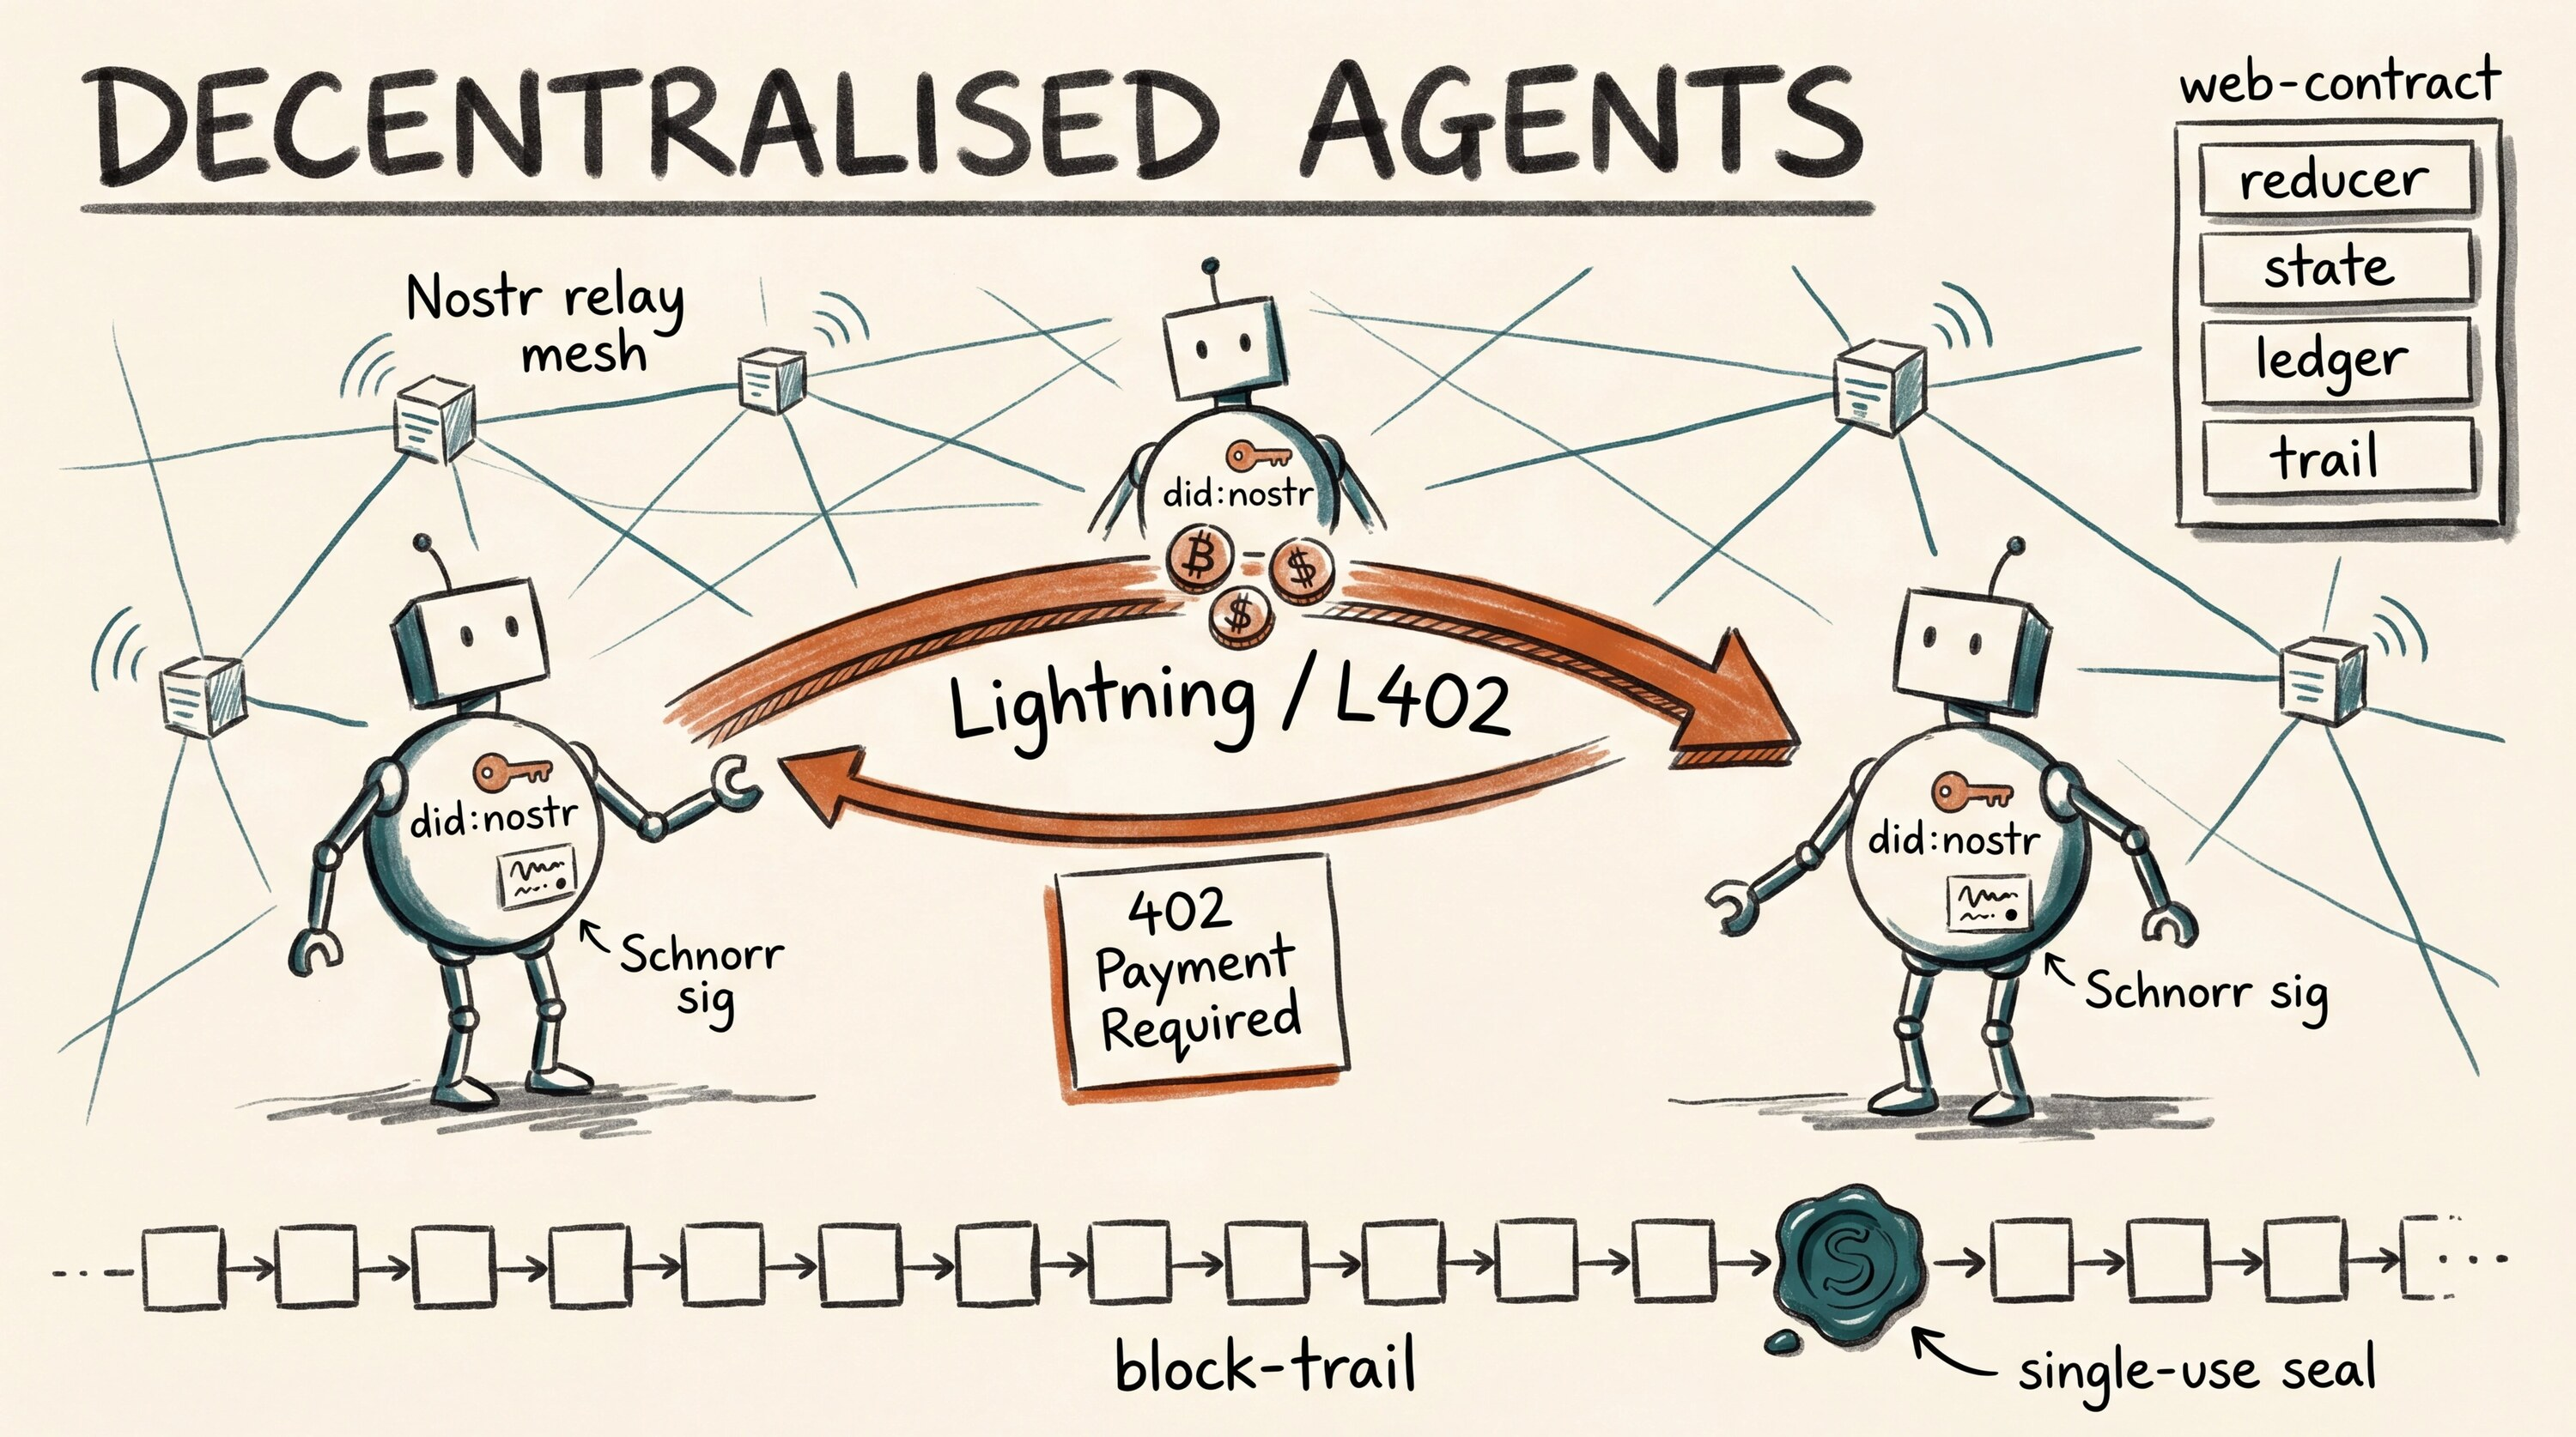
\includegraphics[width=0.86\textwidth]{hero-agentic-mycelia.jpg}

\vspace{0.9cm}

{\Large\bfseries Dr.\ John O'Hare}

\vspace{0.4cm}

{\large\color{navyblue!70!black}
DreamLab AI Consulting Ltd\\
DreamLab, Fairfield, Eskdale}

\vspace{1.5cm}

{\large Third Edition --- July 2026}
\vspace{0.3cm}

{\small\color{navyblue!60!black}First edition, as \textit{The Coordination Collapse}: April 2026}

\vspace{2cm}

{\color{accentgold}\rule{\textwidth}{2pt}}

\vfill

{\small\color{navyblue!50!black}
A book-length thesis in five movements: an emerging coordination problem,\\
the research mapping its solution space across four interaction surfaces,\\
the VisionFlow ecosystem built to occupy that space, an honest gap analysis\\
of theory against running code, and the evaluation plan the gaps demand.}

\end{center}
\end{titlepage}

% ─── Front Matter ────────────────────────────────────────────────────────────
\frontmatter
\pagestyle{plain}

\tableofcontents
\listoffigures
\listoftables

% ─── Main Matter ─────────────────────────────────────────────────────────────
\mainmatter
\pagestyle{fancy}

\chapter{Introduction}
\label{ch:introduction}

\epigraph{For two thousand years, organisations paid a coordination tax: layers of people whose main job was routing information between other people. AI drops the cost of that routing towards zero. What performs the coordination function, once hierarchy no longer has to, is the question this book takes up.}{}

\section{A Function Changes Hands}

By the middle of 2026, a function that organisations spent two thousand years building is quietly changing hands. Coordination (the routing of information, the checking of work, the deciding of who does what next) is passing to software, and it is passing faster than the structures built to govern people can follow. Over half of the people using generative AI at work do so without telling their employer \parencite{Mollick2023SecretCyborgs}. Shadow adoption rose 156 per cent in two years, and the average large organisation now runs around 1,200 AI applications that nobody in charge approved \parencite{IBM2025}. The adoption is real, the productivity is real, and almost none of it is visible to the managers nominally accountable for it. A workforce has acquired a capability its own institutions have not yet admitted exists, and it acquired it from the bottom up.

The capability is uneven in a way that makes trust and distrust both dangerous. A preregistered experiment with 758 consultants found a jagged frontier: on tasks inside the model's range, AI lifts quality and speed sharply; a short step outside it, the same tool quietly degrades the work while sounding every bit as fluent \parencite{DellAcqua2026}. Wholesale automation is reckless across that frontier, and passive oversight is worse, because human vigilance decays exactly as the tool improves and the failures grow quieter. That frontier is also moving under everyone's feet. The first benchmark to grade AI deliverables against what a paying client would accept, rather than against a synthetic score, recorded the automation rate for economically valuable freelance work climbing from 2.5 to 16.1 per cent in under eight months \parencite{CAIS2026RLI}.

An agent that can act unattended is also an agent that can be steered, and a group of them fails in ways a single tool never could: a documented taxonomy of fourteen failure modes spanning bad specification, agents talking past each other, and verification that never happens \parencite{Cemri2025}. Put the pieces together and the shape is a coordination function moving to machines with no matching move in the governance around them. The consequence is concrete rather than theoretical: a single crafted instruction hidden inside a document an agent reads can turn a helpful assistant into an exfiltration tool, and a group of agents gives that failure more doors to enter by and more places to hide. Four things that current agent frameworks treat as add-ons have to become infrastructure instead: a verifiable identity for every actor, disclosure when an actor is an agent, a human who can still be reached and can still say no, and a receipt an adversary can check. Without those, the collapse is merely endured. With them, it can be managed.

\section{VisionFlow, Named}

VisionFlow is the working answer this book puts forward and then grades. It is a governed mesh where AI agents work beside people under four guarantees made first-class rather than bolted on: a verifiable identity for every actor, disclosed agency, human-held escalation, and receipts an adversary can check. It presents four surfaces onto one shared substrate: a forum where governance decisions get made, a desktop that observes and lays out the work, a headset that extends it into shared space, and a voice that addresses it aloud. Under all four runs a single cryptographic identity spine, and each actor keeps its own data in a personal pod, so the value a person creates settles to that person and leaves with them when they go. Terms of art such as identity spine, pod and ontology are collected in the glossary at Appendix~\ref{ch:glossary}, defined on first heavy use.

The organising idea is trust built by verification rather than assurance, and it resolves into three things a buyer can name. First, governed and auditable coordination: every agent action is signed, the roughly nine routine decisions in ten flow without a human, and the tenth that needs judgment escalates cleanly to a named person, while any later decision traces back through an unbroken chain to the source data it rested on. Governance reads as an accelerant, not a bottleneck, and the audit trail is the compliance story regulated buyers already pay for. Second, self-sovereign identity and data: one key is login, access control, payment account and provenance author at once, and if you leave the mesh you take your data with you, which is precisely what lets parties who will never pool their data collaborate anyway, the contract lab running a screen it is paid for without ever seeing the client's target list. Third, shared meaning a machine can act on: a formal ontology yields provably correct entailments where a language model would guess, which removes the failure where two agents mean different things by the same word, rendered as a live spatial graph a room full of people can inspect together.

Two honesties belong on this page, before the detail can ambush a sceptic. Single-operator and team deployments run today; cross-organisation federation is designed and still being built, and this book marks that line every time it matters. And the stack is not a slide deck. It runs daily at DreamLab on a live graph of some seventeen thousand nodes, its value layer is a working peer-to-peer exchange with an order book and a liquidity pool rather than a metering diagram, and the parts that are still scaffolding are named as scaffolding wherever they appear.

Three readers can each take a different reason to continue. For the executive weighing the bet, the moat is that a competitor cannot retrofit verifiable identity, portable data and provenance onto a stack that was never built to carry them. For the leader accountable for governance or audit, every consequential action leaves a human-signed, checkable trail. For the engineer, the whole thing hangs off a single keypair that is identity, access-control principal, payment account and provenance author in one. The argument targets knowledge-work organisations of roughly fifty to five hundred people, the design range the mesh itself claims in Chapter~\ref{ch:three-models}, where the coordination tax is most visible; heavily regulated and physical-process industries face constraints this book acknowledges without fully resolving.

\section{An Argument and Its Working Proof}

This book is two things at once, and it reads more cleanly once that is said out loud. It is an argument, that hierarchy was an information-routing protocol and that AI has made the old routing obsolete, and it is the working proof of that argument, a running system built to occupy the space the argument clears. Neither half is decoration for the other. The argument alone would be a think-piece with nothing to test it; the system alone would be a product brochure with nothing to justify its shape. VisionFlow is offered as the proof of the argument; the selling can wait for a different book.

\begin{evidencebox}[title={How This Book Was Verified}]
The claims about VisionFlow in Part~\ref{part:visionflow} and the scorecard in Part~\ref{part:assessment} were not written from memory. The central assessment, Chapter~\ref{ch:gap-register}, was produced by a twelve-agent analysis mesh: one agent extracted what the canon actually claims, four surveyed the shipping code surface by surface, three researched the outside literature on independent search engines so no single index shaped the theory, and four adversarial judges ranked canon and code against that literature. Every closure was then re-checked by a verifier holding a refutation mandate and drawn from a different model family than the agent that produced the work. That refutation pass caught twelve false closures across three waves and sent them back, including one fabricated claim in a verifier's own report. An author auditing his own system is the standing objection to the whole exercise; those twelve caught closures are the evidence that, run against itself with a mandate to refute, the discipline has teeth. Where later evidence overturned an earlier claim, the book says so at the point the original claim was made.
\end{evidencebox}

\section{Five Parts}

The argument runs in five parts. Part~\ref{part:problem} diagnoses the condition: a coordination function passing to machines faster than institutions can adjust, a frontier whose edges stay jagged, and a vigilance that decays as the tools improve. Part~\ref{part:solution-space} surveys what could replace the lost function, from the transaction-cost economics of agent coordination through to the four surfaces where humans and agents actually meet. Part~\ref{part:visionflow} gives each component of VisionFlow its own chapter, written against that research and stating its maturity plainly. Part~\ref{part:assessment} is the reckoning, a gap register that crosses outside theory, stated doctrine and code-verified practice and types every gap by which of the three fell behind. Part~\ref{part:next-steps} converts the reckoning into dated, falsifiable commitments and an evaluation lens for the next edition.

The book also has a printed, dated pre-history: a 2022 synthesis \parencite{OHare2022Convergence} that read decentralised identity, machine-to-machine value and the coming model wave as one converging system, several of whose maps are now running code. Chapter~\ref{ch:2022-wager} scores every headline call that book made against 2026, misses first. One disclosure travels with it: the name VisionFlow first appears in that 2022 book on an unrelated gaze-personalisation idea, and the system described here reuses the name, not the design.

Read the two halves together and the wager is a plain one. The honest version of this system, graded in public against its own claims, is the more credible one, and that is the bet the rest of the book is written to pay out.


\part{An Emerging Problem}
\label{part:problem}

\input{chapters/02-historical-context}
\input{chapters/03-collapse-point}
\chapter{The Jagged Frontier}
\label{ch:jagged-frontier}

\epigraph{The person who knows where the frontier is jagged in their domain is the most valuable person in the organisation.}{}

\section{Why Wholesale Automation Is Reckless}

If coordination is now computationally cheap, the logical next question is whether to simply replace the hierarchy with AI. Several prominent voices (most notably \textcite{DorseyBotha2026}) propose exactly this. But the evidence reveals that the boundary between what AI can do and what it cannot is dangerously unpredictable. This boundary is the single most important concept in the entire coordination collapse thesis.

\section{The BCG Experiment}

The \meshterm{jagged technological frontier} was identified and named by \textcite{DellAcqua2026} in what remains the most rigorous field experiment on human-AI collaboration in knowledge work. The study was preregistered, conducted with 758 consultants at Boston Consulting Group: not a laboratory convenience sample, not a blog post, but a controlled experiment with one of the world's premier professional services firms.

The researchers assigned consultants to eighteen realistic consulting tasks and measured the results against a control group working without AI assistance. The findings established two sharply distinct performance regimes.

\begin{evidencebox}[title={Inside the Frontier}]
For the eighteen tasks that fell within AI capability:
\begin{itemize}
  \item Consultants using GPT-4 completed \textbf{12.2 per cent more tasks}
  \item They finished \textbf{25.1 per cent faster}
  \item They produced \textbf{40 per cent higher quality} output, as rated by blind evaluators
\end{itemize}
\end{evidencebox}

\begin{cautionbox}[title={Outside the Frontier}]
For a complex business judgement task requiring integration of real-world context:
\begin{itemize}
  \item AI users were \textbf{19 per cent less likely} to produce correct solutions than those working without AI
  \item The frontier was unpredictable: adjacent tasks that appeared similar fell on opposite sides
\end{itemize}
\end{cautionbox}

The metaphor of a ``jagged'' frontier is precise. Unlike a smooth gradient where tasks become progressively harder for AI, the boundary is irregular and counterintuitive. Two tasks that appear nearly identical from the outside (similar in domain, complexity, and required expertise) can fall on opposite sides of the frontier. One is dramatically improved by AI assistance; the other is degraded by it. There is no reliable way to determine which is which without empirical testing.

\begin{figure}[h]
\centering
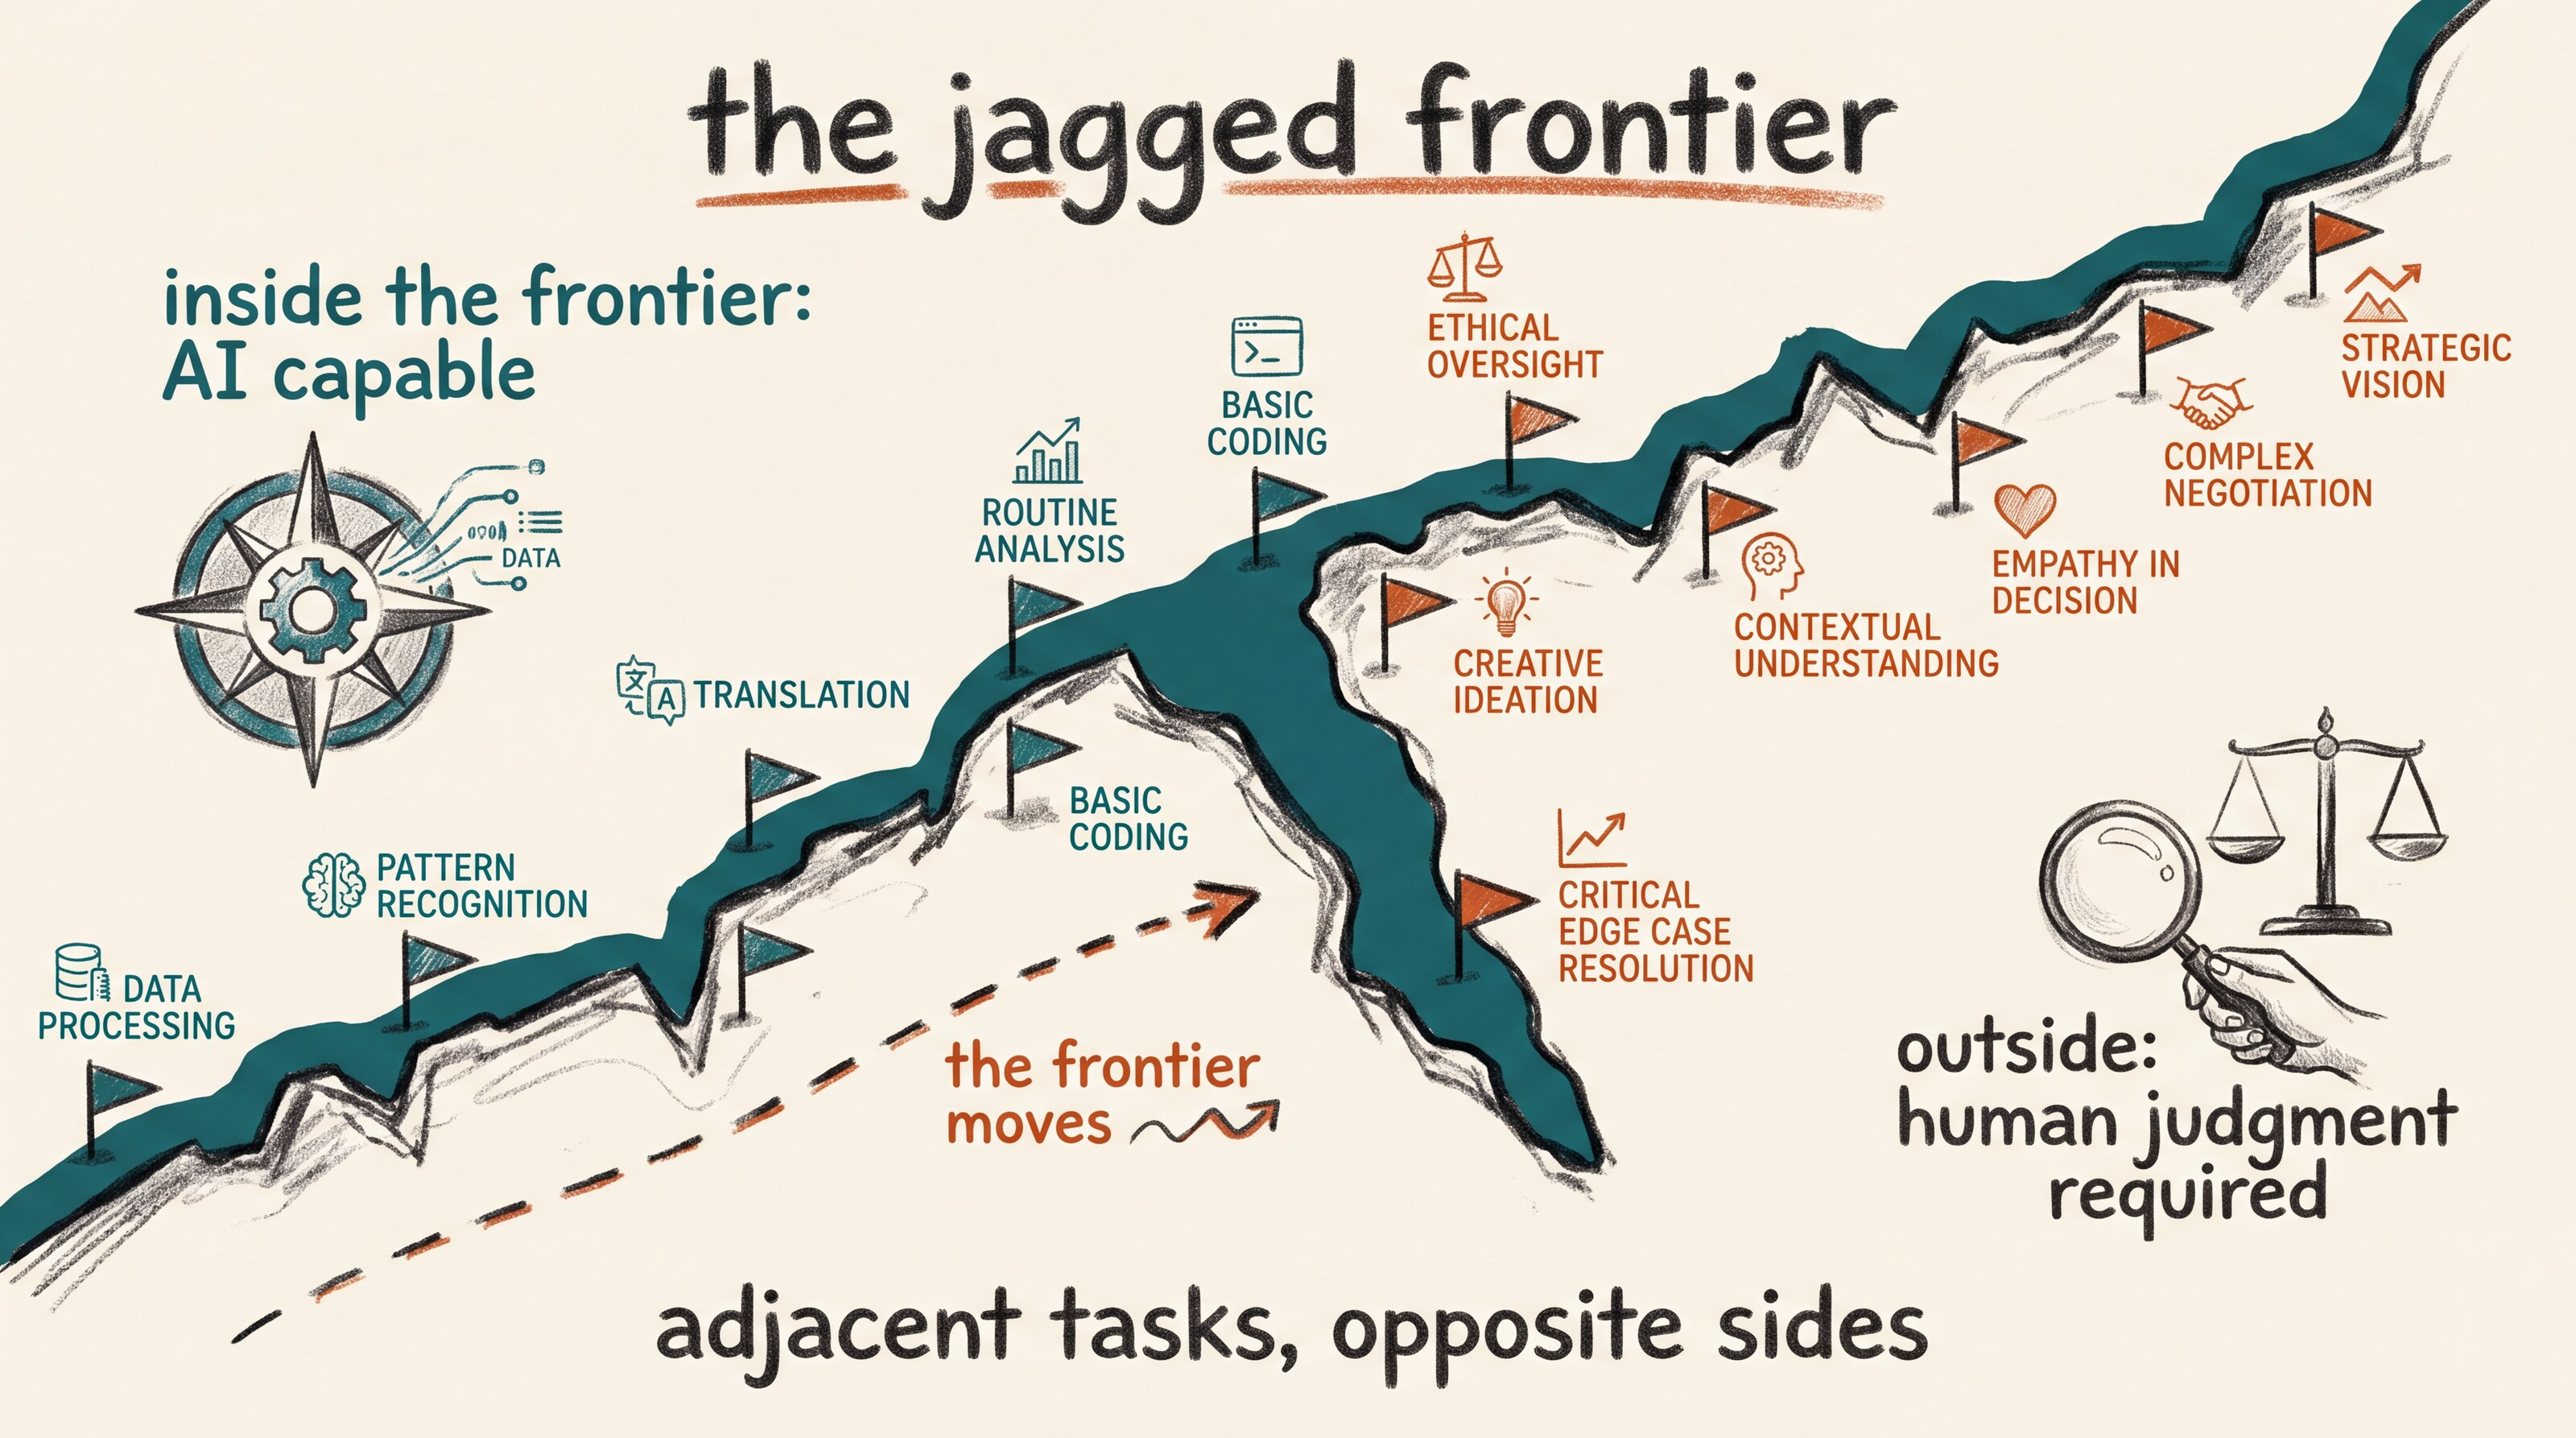
\includegraphics[width=0.92\textwidth]{nb-jagged-frontier.jpg}
\caption{The jagged technological frontier. Adjacent tasks fall on opposite sides of an irregular, moving boundary; the only reliable map is empirical testing in your own domain.}
\label{fig:jagged-frontier}
\end{figure}

\section{The Skill-Levelling Effect}

The BCG experiment revealed a second finding with profound implications for organisational design. AI did not improve all consultants equally:

\begin{itemize}
  \item Bottom-half performers saw a \textbf{43 per cent performance jump} with AI assistance.
  \item Top performers improved measurably but by a smaller margin.
  \item AI compressed the talent distribution, bringing lower-performing consultants much closer to the performance of their higher-performing colleagues.
\end{itemize}

This skill-levelling effect changes what managers are managing. In a pre-AI organisation, individual performance variation is a primary concern: identifying, developing, and retaining high performers is a core management function. When AI compresses the performance distribution, the variation between individuals shrinks. The manager's value shifts from talent differentiation to system coherence, ensuring that the newly capable workforce is pointed at the right problems and that AI assistance is applied where it helps rather than where it harms.

\section{Three Collaboration Modes}

A follow-up study by \textcite{Randazzo2024}, conducted with 244 BCG consultants, identified three distinct modes of human-AI collaboration. These modes are not merely descriptive; they are predictive of performance outcomes.

\begin{table}[h]
\centering
\caption{Human-AI collaboration modes and performance outcomes}
\label{tab:collaboration-modes}
\begin{tabularx}{\textwidth}{l L{5cm} X}
\toprule
\textbf{Mode} & \textbf{Description} & \textbf{Performance} \\
\midrule
Centaurs & Clear division of labour. The human performs tasks where human judgment is strongest; the AI handles tasks inside the frontier. Distinct handoff points between human and machine. & High \\
\addlinespace
Cyborgs & Continuous interleaving. Human and AI work on the same analysis, passing work back and forth across the frontier boundary. No clean separation of responsibilities. & High \\
\addlinespace
Self-Automators & Wholesale delegation to AI with minimal oversight. The human provides the initial prompt and accepts the output with little or no review. & Lowest \\
\bottomrule
\end{tabularx}
\end{table}

Both Centaurs and Cyborgs outperformed solo humans and solo AI. Self-Automators produced the weakest results, precisely because wholesale delegation triggers the vigilance problem examined in the next chapter.

\begin{keyinsight}[title={The Organisational Design Implication}]
This taxonomy maps directly onto the three organisational models examined in Chapter~\ref{ch:three-models}:
\begin{itemize}
  \item Block's intelligence layer model creates \textbf{Self-Automator organisations}, delegating coordination to an AI world model.
  \item Every's agent colony model creates \textbf{Cyborg organisations}: continuous interleaving between human and personal agent.
  \item The Dynamic Agentic Mesh creates \textbf{Centaur organisations}: clear boundaries with judgment brokers at the handoff points.
\end{itemize}
The evidence shows that Self-Automators perform worst. This is the empirical case against wholesale delegation.
\end{keyinsight}

\section{Quantifying the Frontier: The Remote Labor Index}

The BCG experiment and its successors establish that the frontier is jagged. They do not, on their own, tell us how fast the frontier is moving, or how far it has moved. That longitudinal, quantitative measurement now exists, and it changes the shape of the argument.

The \meshterm{Remote Labor Index} (RLI) \parencite{RLI2025}, published by the Center for AI Safety and Scale AI as arXiv:2510.26787 in October 2025, tests AI models against real, economically valuable freelance projects: 3D modelling and CAD, architecture, graphic design, video and audio editing, data analysis, and web-application programming. Every project is judged by human evaluators against a gold-standard deliverable produced by a paid professional. This is a materially harsher bar than the task-level benchmarks that dominate AI capability reporting. The RLI does not ask whether a model can pass a coding exercise or answer a reasoning puzzle; it asks whether the model's output would be accepted by a paying client in place of a professional's work.

At launch, the best-performing model automated 2.5 per cent of RLI projects to that standard. The July 2026 update \parencite{CAIS2026RLI} reports a step change: Claude Fable 5 at 16.1 per cent, Claude Opus 4.8 at 8.3 per cent, and GPT-5.5 at 6.3 per cent. In the Center for AI Safety's own words: ``The frontier has more than quadrupled in under eight months, a concrete signal of how quickly economically capable AI agents are advancing.''

The update's example deliverables illustrate what 16.1 per cent automation looks like in practice: photorealistic renders of an engagement ring redesign, a flat-design 2D animated advertisement for a fictional tree-services company, and dimensioned floor plans with accompanying photorealistic renders. These are not toy tasks. They are the kind of whole-deliverable freelance work that supports real careers. CAIS is explicit about the limits of what has been achieved: ``Today's AI still falls short of professional quality on most projects.''

\begin{keyinsight}[title={The First Longitudinal Quantification of the Jagged Frontier}]
The RLI is the first instrument that tracks the jagged frontier longitudinally, at client-quality standard, across whole deliverables rather than sub-tasks. It deserves to be read two ways at once, and the report insists on holding both readings simultaneously rather than collapsing into either.

\textbf{Read one:} 16.1 per cent means the human remains indispensable on roughly five of every six projects. The gold-standard bar (would a paying client accept this?) is not being cleared for the overwhelming majority of real freelance work. Professional-quality completion is still the exception, not the rule.

\textbf{Read two:} the boundary moved more than sixfold in eight months. A frontier that automates one project in forty in October 2025 and one project in six by July 2026 is not moving on the multi-year timescale that organisational change management assumes. It is moving on a timescale shorter than most transformation programmes.

Both readings are correct, and the tension between them is not a contradiction to be resolved; it is the terrain the judgment broker (Chapter~\ref{ch:role-transformation}) operates on. Tasks are not jobs: automating 16.1 per cent of freelance \emph{projects} at professional quality is a different claim from automating 16.1 per cent of freelance \emph{work}, let alone 16.1 per cent of jobs. The RLI measures whole deliverables against a client-acceptance bar, which makes it a better proxy for job-level displacement than task-level benchmarks, but it is still a proxy, not a labour-market outcome. The space between ``the human is still needed five times out of six'' and ``the boundary moved sixfold in eight months'' is exactly the space that frontier-mapping expertise exists to navigate. Knowing where today's one-in-six lives, and how fast it is becoming one-in-five, is the scarce and valuable knowledge this report has been calling the judgment broker's domain since the opening chapters.
\end{keyinsight}

The RLI is a measure of capability under harsh, client-quality evaluation. A complementary measure (of capability under a looser, time-based standard) comes from METR's task-horizon work. METR's metric asks how long a task a frontier model can complete with 50 per cent reliability, calibrated against the time a human expert would need. That horizon has doubled roughly every seven months since 2019, and the trend has recently accelerated \parencite{METR2026}. Claude Opus 4.6 was measured at approximately 14.5 human-expert hours when added to METR's tracker in February 2026, meaning frontier models now reliably complete, half the time, tasks that would occupy a skilled professional for nearly two working days.

Both metrics point the same direction and both come with the same caveat. These are benchmark capabilities, measured under conditions designed to isolate the model's raw ability. Deployed capability is narrower: real-world use is gated by system integration, permission scoping, and the handling of exceptions that a benchmark does not surface. The RLI and METR describe how fast the frontier is moving in principle. Chapter~\ref{ch:vigilance} and the mesh architecture in later chapters describe what it takes to move it safely in practice.

\section{Why the Frontier Matters for Governance}

The jagged frontier has four implications that recur throughout this report.

\textbf{First, it invalidates wholesale automation.} If you cannot predict in advance which tasks AI will improve and which it will degrade, a strategy of replacing human judgment with AI judgment is not bold --- it is uninformed. The 19 per cent performance degradation on tasks outside the frontier is not a temporary limitation that will be resolved by the next model generation. It is a structural feature of deploying any system at the boundary of its capability.

\textbf{Second, it defeats one-time change playbooks.} The frontier moves as models improve. A task that falls outside the frontier with GPT-4 may fall inside it with the next generation. Conversely, increased model capability can create new failure modes at different points on the boundary. A change management plan that maps the frontier today will be outdated within months. This demands continuous adaptation, not phased transformation.

\textbf{Third, it creates a new form of expertise.} The person who knows where the frontier falls in their specific domain (who has mapped which tasks are reliably improved by AI and which are reliably degraded) holds knowledge that is genuinely scarce and strategically valuable. This is the \meshterm{judgment broker} role developed in Chapter~\ref{ch:role-transformation}. It is not a euphemism for a diminished middle management function. It is a description of expertise that did not exist before the frontier existed.

\textbf{Fourth, it demands active engagement, not passive oversight.} The standard response to AI risk (``keep a human in the loop'') assumes that the human will maintain vigilance. The next chapter demonstrates why that assumption fails, and what it means for organisational design.

\section{The Frontier Is Dynamic}

It is important to note a limitation of the evidence. The BCG experiment used GPT-4, now several model generations behind current frontier models. The specific task boundaries identified in 2023 have almost certainly shifted. Some tasks that fell outside the frontier are now inside it; others may have developed new failure modes as model capabilities have changed. The April 2026 edition of this report flagged this as an open problem: the BCG task map was already outdated, and no instrument existed to re-measure the frontier as models improved.

That instrument now exists. The Remote Labor Index, tracked from its October 2025 launch through the July 2026 update, is exactly the longitudinal re-measurement this chapter previously had to do without. It confirms both halves of the original claim at once. The frontier moves fast: a sixfold improvement in eight months is not a rounding error, it is a different pace of change than most organisational planning horizons assume. And the frontier remains jagged: at 16.1 per cent automation, professional-quality completion of a whole freelance deliverable is still the exception rather than the rule, across every category the index measures. The GPT-4-era task map is out of date, as flagged; what has changed since is that the report no longer has to rely on a single snapshot to make the point. Continuous measurement (the RLI updated every few months, METR's tracker updated as models are released) is now doing the job that a one-off field experiment could only gesture at.

The implication is unchanged, and sharper for it: organisations need people who actively probe the boundary rather than assuming they know where it is. The frontier will always be jagged because AI capability will always be unevenly distributed across the task space of any complex domain. What is new is that the rate of movement is now measured, not merely inferred, and the rate is fast enough that a frontier map drawn this quarter should be assumed stale by the next.

The publication of the BCG study in \emph{Organization Science} in March 2026 \parencite{DellAcqua2026} provides the peer-reviewed validation that the working paper lacked. The jagged frontier is no longer a provocative hypothesis. It is an established finding in the organisational science literature --- and, as of the Remote Labor Index, a finding with a running clock attached to it.

\chapter{The Vigilance Problem}
\label{ch:vigilance}

\epigraph{The better AI becomes, the harder it is to maintain vigilance. Errors from high-performing AI are especially dangerous because outputs are polished, fluent, and plausible --- making hallucinations and boundary failures nearly invisible to casual review.}{}

\section{Why ``Human in the Loop'' Is Not Enough}

The standard response to the jagged frontier is to keep a human in the loop. Every governance framework, every responsible AI policy, every enterprise deployment guide says it: humans will oversee the AI. The phrase has become a mantra --- a reassurance offered to boards, regulators, and employees alike that human judgment remains the final arbiter.

The evidence says otherwise. Oversight degrades as AI quality improves, and it degrades in precisely the conditions where reliable oversight matters most.

\section{Falling Asleep at the Wheel}

\textcite{DellAcqua2023} conducted a field experiment with HR recruiters that produced a finding both counterintuitive and deeply consequential for organisational design. The study examined how the quality of AI assistance affected the quality of human decision-making.

\begin{evidencebox}[title={The Counterintuitive Finding}]
Recruiters given \textbf{high-quality} AI made \textbf{worse decisions} than those given low-quality AI or no AI at all.
\begin{itemize}
  \item Those with superior AI spent less time per resume, followed recommendations uncritically, failed to improve over time, and missed strong candidates.
  \item Those with inferior AI stayed alert, developed better critical judgement, and improved their independent evaluation skills.
\end{itemize}
\end{evidencebox}

The mechanism is straightforward once stated. When AI produces consistently excellent output, the human reviewer has little reason to scrutinise any individual output carefully. Each correct recommendation reinforces the habit of acceptance. The cognitive effort required for careful evaluation is substantial, and the reward for that effort --- occasionally catching a rare error --- is small and unpredictable. The rational response, at the level of moment-to-moment cognitive allocation, is to reduce scrutiny. The human falls asleep at the wheel.

This is not a failure of individual discipline. It is a predictable response to the statistical structure of the task. The better the AI, the lower the base rate of errors, and the harder it becomes for a human monitor to maintain the vigilance required to catch the errors that do occur.

\section{The Quality Paradox}

The vigilance problem creates a perverse dynamic: the conditions under which AI most needs oversight are precisely the conditions under which oversight is least reliable.

When AI output is mediocre or inconsistent, human reviewers remain engaged. They catch errors, develop independent judgment, and contribute genuine value to the process. The human-in-the-loop model works because the human is cognitively active.

When AI output is excellent and consistent --- which is the goal of every AI deployment --- human reviewers disengage. They become rubber-stampers. The errors they miss are not the obvious ones (those were caught by the AI itself) but the subtle, contextual, boundary-case errors that only a cognitively engaged domain expert would detect. These are precisely the errors that matter most.

\begin{keyinsight}
The standard enterprise governance model --- deploy high-quality AI and overlay it with human review --- contains a self-defeating dynamic. The better the AI, the worse the review. This is not a solvable problem within the ``human in the loop'' paradigm. It requires a different architectural approach.
\end{keyinsight}

\section{Implications for Organisational Design}

The vigilance problem has four direct implications for any organisation deploying AI at scale.

\subsection{Passive Oversight Degrades}

A governance model that relies on humans reviewing AI output after the fact --- the audit committee model, the quarterly review, the approval workflow --- will produce steadily declining oversight quality as AI quality improves. The humans in these roles will not be aware of their declining performance, because the visible output will appear consistently excellent. The errors will be invisible until they compound into a failure large enough to attract attention.

\subsection{Active Engagement Is Required}

The judgment broker must be \emph{actively engaged} with the AI system, not passively overseeing it. This means the role must include tasks that require genuine cognitive effort --- not merely confirming that an output ``looks right,'' but probing the reasoning, testing the boundaries, and deliberately seeking failure modes.

\subsection{Deliberate Friction Is a Design Requirement}

The mesh must be designed to keep humans cognitively active at the jagged frontier. This is counterintuitive: most system design aims to reduce friction and make workflows smoother. The vigilance problem demands the opposite. The system should surface genuine edge cases and ambiguous decisions. It should present the human with problems that require thought, not with confirmation dialogs that require a click. The human must be kept sharp, not comfortable.

\subsection{Governance Must Be Continuous}

Periodic review --- quarterly audits, annual risk assessments, monthly committee meetings --- is structurally inadequate. The vigilance problem operates at the level of individual decisions made in real time. Governance must be embedded in the flow of work, not bolted on at intervals. Chapter~\ref{ch:governance} develops this principle into the concept of declarative governance, where policy enforcement is architectural rather than procedural.

\section{Calibrating Oversight: Evidence from the Field}

The argument so far has been diagnostic: passive review degrades, and the mesh should be designed to keep humans cognitively active rather than comfortable. What has been missing is field evidence on which oversight architectures actually deliver that active engagement at scale. The Stanford Digital Economy Lab's Enterprise AI Playbook \parencite{Pereira2026Playbook} supplies it.

\textcite{Pereira2026Playbook} classified 51 mature, production-grade AI deployments by their oversight model. Three patterns recurred: \textbf{escalation}, in which the AI system handles 80 per cent or more of volume autonomously and humans review only flagged exceptions; \textbf{approval}, in which a human reviews every output before it takes effect; and \textbf{collaboration}, in which human and AI work continuously on the same task. The productivity gap between the first two was not marginal. Escalation-based operating models produced 71 per cent median productivity gains; approval-based models produced roughly 30 per cent.

\begin{evidencebox}[title={Escalation versus Approval: The Field Evidence}]
\begin{itemize}
  \item \textbf{Escalation} (AI autonomous on 80+ per cent of volume, humans handle exceptions): \textbf{71 per cent} median productivity gain.
  \item \textbf{Approval} (human reviews every output): \textbf{$\sim$30 per cent} median productivity gain.
  \item One 80/20 content-production deployment with zero-error tolerance still cut time-to-market from 7 weeks to 6 hours --- escalation and zero tolerance are not mutually exclusive when the escalation boundary is drawn correctly.
\end{itemize}
\end{evidencebox}

Part of this gap is task selection: escalation architectures were deployed on high-volume, recoverable work, while approval architectures were reserved for regulated or zero-error-tolerance domains where the Playbook's authors identify four legitimate reasons for retaining human review --- zero error tolerance, regulatory mandate, enterprise risk exposure, and the need for a continuous improvement feedback loop back into the system. Approval workflows are not a mistake in those domains. They are frequently the correct design choice.

But task selection does not explain away the finding; it sharpens it. The design lesson is not that oversight is optional wherever volume is high. It is that the vigilance problem's own logic --- review everything and you review nothing, because uniform review is exactly the condition under which human attention habituates and disengages --- has a field-tested architectural answer. That answer is not blanket approval workflows, which this chapter has already shown degrade into rubber-stamping precisely as the underlying AI improves. It is well-designed escalation, which concentrates scarce human attention on the cases that are genuinely novel, ambiguous, or high-stakes, and lets routine volume pass without consuming the cognitive resource that matters.

\begin{keyinsight}[title={Deliberate Friction, Operationalised}]
This is the operational form of the deliberate-friction principle introduced earlier in this chapter. A judgment broker asked to approve every output learns to stop reading them. A judgment broker whose attention is reserved for the exceptions an escalation architecture surfaces is, by construction, being shown the cases that require thought. Escalation is deliberate friction implemented as a routing decision rather than an interface design choice.

This connects directly to two constructs elsewhere in this report. The HITL Precision KPI (Chapter~\ref{ch:new-kpis}) measures exactly what an escalation architecture is designed to produce: a high proportion of human interventions that materially change the outcome, rather than interventions that merely rubber-stamp an already-correct AI decision. And the judgment broker role (Chapter~\ref{ch:role-transformation}) is, in this light, not a euphemism for a smaller reviewing job --- it is the human half of an escalation boundary, positioned precisely where the Playbook's evidence says human attention produces the largest return.
\end{keyinsight}

The practical design question this raises --- and the one the mesh architecture must answer per deployment --- is where the escalation boundary should sit: what volume of decisions can be handled autonomously, what triggers an exception, and what evidence must accompany an escalated case so the human reviewer can act on it rather than merely rubber-stamp it under a different name. Getting that boundary wrong in either direction reproduces the vigilance problem: too permissive, and genuine errors pass unreviewed; too conservative, and the system reverts to the approval model this evidence shows underperforms.

\section{The Atrophy Prediction}

\textcite{Gartner2025} predicts that by 2026, 50 per cent of organisations will require ``AI-free'' skills assessments --- evaluations of employee capability conducted without AI assistance --- specifically because of critical-thinking atrophy from generative AI dependency.

This prediction reflects a growing awareness that the vigilance problem is not an edge case. It is the central challenge of human-AI governance. If human cognitive capability degrades as AI capability improves, and if that degradation is invisible to both the individual and the organisation until a significant failure occurs, then the standard model of AI deployment --- train the AI, deploy the AI, have humans oversee the AI --- is fundamentally unsafe at scale.

\begin{cautionbox}[title={Design Implication for the Agentic Mesh}]
The judgment broker role must include deliberate friction --- tasks that require active engagement, not merely approval. The mesh should surface genuine edge cases and ambiguous decisions, not filter them out. The human must be kept cognitively sharp, not merely present in the process.

This is a design requirement, not a training problem. No amount of training in ``critical thinking'' will overcome the cognitive dynamics that cause vigilance to degrade. The system architecture must compensate for the predictable tendency of humans to disengage from high-quality automated output.
\end{cautionbox}

\section{The Vigilance Problem at the Agent Layer}

Everything so far has treated vigilance decay as a problem of human attention directed at a stable, if improving, AI system. \parencite{Khanal2026} shows the problem does not stop there: the agents themselves become less reliable, in a specific and counterintuitive way, exactly as they become more capable.

Across 23,392 episodes spanning ten models, the frontier models --- the most capable systems tested --- showed the highest meltdown rates of any tier, up to 19 per cent on long-horizon tasks. This is not a paradox once the mechanism is examined: a more capable model is more willing to attempt ambitious, multi-step strategies rather than conservative, narrowly-scoped ones, and ambitious multi-step strategies have more places to spiral out of control before they fail. Capability does not translate uniformly into reliability; it can translate into more ambitious failure.

A second finding compounds the first. Memory scaffolds --- the mechanism most naturally reached for when an agent's context runs out mid-task --- \emph{universally hurt} long-horizon performance in this study, across every model tested. The intuitive fix for an agent losing track of a long task is to give it more memory of what it has already done. The evidence says this makes long-horizon performance worse, not better.

\begin{cautionbox}[title={Trust-the-Model Optimism Is Not a Strategy}]
Read together, these two findings extend the vigilance problem down into the agent layer itself. It is not only that humans become less reliable overseers as AI improves; it is that AI agents become less reliable executors, in more ambitious and less predictable ways, as they become more capable --- and the most obvious engineering fix does not help. This is direct evidence against any design that assumes a sufficiently capable model can be trusted to self-manage a long-horizon task with a lighter oversight touch than a less capable one would need. The opposite is closer to true.

This strengthens the case, made throughout this chapter, for architectural rather than optimistic vigilance: continuous Trust Variance monitoring and well-designed escalation boundaries (Chapter~\ref{ch:new-kpis}) that catch a meltdown in progress, rather than governance that relaxes as models improve on the assumption that better models need less watching.
\end{cautionbox}

\section{What This Means for the Three Models}

The vigilance problem is the lens through which the three organisational models in the next chapter should be evaluated.

Block's intelligence layer model, which delegates coordination to an AI world model with human oversight, is maximally exposed to the vigilance problem. The better the world model works, the less likely humans are to catch the cases where it fails. The 95 per cent figure --- the proportion of AI-generated code at Block that still requires human modification --- suggests that the system is not yet good enough to trigger full vigilance decay. But that is a temporary reprieve. As the system improves, vigilance will decline, and the remaining 5 per cent of cases where human intervention is critical will receive less attention, not more.

Every's agent colony model partially mitigates the problem through personal relationship: because the agent is ``mine,'' there is reputational incentive to monitor its output. But this mitigation weakens at scale. When every employee has an agent, and when agents interact with other agents, the reputational feedback loop becomes diffuse. The ant death spiral --- agents responding to agents in loops --- is a manifestation of vigilance failure at the system level.

The Dynamic Agentic Mesh addresses the vigilance problem architecturally, through embedded governance, continuous trust variance monitoring, and a judgment broker role designed around active engagement rather than passive review. Whether this architectural approach succeeds at scale is an open question. That it addresses the right problem is supported by the evidence --- including, now, field evidence: the escalation architectures documented in \textcite{Pereira2026Playbook}, which produced the strongest productivity gains of any oversight model studied, are precisely the mesh's core pattern already operating in production.


\part{Mapping the Solution Space}
\label{part:solution-space}

\input{chapters/06-three-models}
\chapter{The Economics of Agent Coordination}
\label{ch:coordination-economics}

\epigraph{The coordination tax does not vanish when the coordinators become software. It migrates into the movement of context --- and it must be engineered.}{}

\section{From Coase to Context}

Ronald Coase's 1937 question --- why do firms exist at all, when markets can in principle coordinate every transaction through price? --- has organised a century of economic thought about the boundary between organisation and market. Coase's answer, sharpened by Oliver Williamson's transaction cost economics in 1985, is that firms exist wherever the cost of coordinating a transaction inside a hierarchy is lower than the cost of coordinating it across a market: search costs, negotiation costs, contracting costs, the risk of opportunism. Where those costs are low, markets win and the transaction stays outside the firm. Where those costs are high, hierarchy wins and the transaction is absorbed inside a boundary of authority.

\textcite{Liu2026} asks what happens to this logic once the parties doing the coordinating are not people but software. His answer, and the central contribution of ``The Organizational Behavior of Agentic AI,'' is that the costly transaction has not disappeared --- it has changed substance. What moves across a boundary between two LLM agents, or between an agent and a human, is not price information or a signed contract. It is context: the state a task carries with it, the evidence that justifies a decision, the memory of what has already been tried, the schema that lets a downstream agent interpret an upstream agent's output. Liu names this cost \meshterm{contextual transaction cost}, and it does for agent collectives what Coase's transaction cost did for firms: it explains when organising several agents together earns its keep, and when it is a species of self-inflicted overhead.

\begin{definitionbox}[title={Contextual Transaction Cost (CTC)}]
The cost, denominated in context rather than money, of moving information, evidence and authority across a boundary between agents (or between an agent and a human) so that a task can proceed. At the level of a single coordination event $e$:

\[
CTC_e = w_\tau \tau_e + w_h H_e + w_c C_e + w_d D_e + w_v V_e + w_g G_e
\]

where $\tau_e$ is token and latency burden, $H_e$ is cross-agent handoffs, $C_e$ is compression loss, $D_e$ is semantic drift, $V_e$ is verification burden, and $G_e$ is governance cost, each scaled by a weight $w$.
\end{definitionbox}

A collective of agents is worth organising --- rather than leaving the task to a single agent --- only when the marginal gains from organising it exceed the marginal costs of doing so:

\[
\Delta G_s + \Delta G_p + \Delta G_d + \Delta G_v > \Delta CTC + \Delta K + \Delta R_g
\]

The left-hand side is the marginal gain from specialisation, parallelism, diversity and verification that a collective can offer over a single agent. The right-hand side is the marginal cost of the contextual transaction tax, the additional compute, and the governance risk that collective organisation introduces. Collective intelligence is not a free upgrade over a single competent agent; it is a trade that has to clear, task by task.

Liu's evidence base deserves to be stated plainly rather than oversold. The paper is computational theorising: 8,000 synthetic knowledge-work tasks tested across seven organisation forms with task fixed effects, corroborated by trace-instrumented runs on real LLM agents performing software repair, long-document question answering, legal review and literature synthesis, and stress-tested with a prompt-free deep-Q-network organisation selector to check the results were not artefacts of hand-tuned prompts. It is a single-author arXiv preprint, posted 29 June 2026, and it has not yet been peer reviewed. Weighed against that: it is, so far as this report's research has found, the first attempt to give the coordination tax --- the mechanism this report has argued for since Chapter~\ref{ch:collapse-point} --- a formal, falsifiable treatment specifically at the level of the agent layer. The report treats it accordingly: as the best available theory, not as settled science.

\section{Human-Imitation Forms Fail in Silicon}

Liu tests seven ways of organising a collective of agents against a single-expert baseline, on 56,000 task-organisation observations with task fixed effects, significant at $p < .001$ for every comparison except market-contract efficiency. Four of the forms are borrowed directly from human organisational design: a pipeline of standard operating procedures, a hierarchy with a manager agent, a committee that debates in free text, and a market that allocates work by contract. Three are native to what agents can do that people cannot: the market-contract form itself, a blackboard architecture where agents read and write to shared, durable state, and an adaptive meta-organisation with a context-aware orchestrator that restructures the collective as tasks demand.

The human-imitation forms lose, and lose by a wide margin.

\begin{table}[h]
\centering
\caption{Liu's seven organisation forms against the single-expert baseline}
\label{tab:liu-forms}
\begin{tabularx}{\textwidth}{L{4.2cm} C{2.6cm} C{2.2cm} X}
\toprule
\textbf{Organisation form} & \textbf{Collective efficiency} & \textbf{Quality} & \textbf{Success probability} \\
\midrule
Pipeline SOP & $-4.28$ & $-6.17$ & $-5.3$pp \\
\addlinespace
Hierarchy manager & $-7.92$ & $-11.49$ & $-11.6$pp \\
\addlinespace
Committee debate & $-12.69$ & $-42.10$ & $-24.0$pp \\
\addlinespace
Market contract & $+0.03$ & $+3.33$ & $+5.8$pp \\
\addlinespace
Blackboard memory & $+7.60$ & $+11.74$ & $+19.5$pp \\
\addlinespace
Adaptive meta-organisation & $+11.43$ & $+14.00$ & $+23.2$pp \\
\bottomrule
\end{tabularx}
\end{table}

All figures in Table~\ref{tab:liu-forms} are point differences from the single-expert agent performing the same tasks \parencite{Liu2026}. The direction of the result is the finding. Pipelines propagate early errors downstream with no mechanism to catch them. Hierarchies force every decision through a manager agent that must compress, and therefore lose, the context beneath it --- repeatedly, at every level of the chain. Committees do worst of all: quality falls by 42.10 points against the single expert, because free-text debate between LLM agents does not produce independent judgement, it produces several instances of the same underlying distribution converging on the same errors together and mistaking agreement for verification.

None of this is a surprise once the mechanism is named. Human hierarchies, pipelines and committees work --- to the extent they work at all --- because of a substrate this report has taken for granted throughout: role expectations that carry social weight, accountability that attaches to a named person, legitimacy that a manager or a committee chair can draw on to make a decision stick. Agents have none of this. Copy the org chart into a collective of language models and you do not get the org chart's benefits; you get its costs without its foundations. A hierarchy becomes repeated context compression. A committee becomes correlated paraphrase dressed as deliberation. A pipeline becomes a conveyor belt for whichever error entered first.

The market-contract form is the only human-imitation form that survives translation into silicon, and it survives narrowly. Markets were never really about hierarchy in the first place: they coordinate through price and contract, which is closer to what an agentic collective can actually enforce --- a specification, a bid, an acceptance criterion --- than the social machinery a hierarchy or a committee depends on.

At the family level, agent-native forms (blackboard, adaptive meta-organisation, and their hybrids) are approximately 395 per cent more efficient than the human-imitation family (pipeline, hierarchy, committee). This report finds a delicious, and slightly uncomfortable, symmetry here. The org chart fails in both directions at once. Chapter~\ref{ch:three-models} makes the case that humans should not be replaced wholesale by an AI hierarchy modelled on Block's Intelligence Layer. Liu's evidence makes the mirror-image case: agents should not be organised as though they were a human hierarchy either. The org chart is not a neutral scaffold that either species can be poured into. It is a specific technology, built for a specific coordination substrate, and neither silicon colonies aping human structure nor human structures automated wholesale by silicon get to skip that constraint.

\section{The Goldilocks Zone of Coordination Cost}

Liu's second headline result answers a question this report has asked in different words since Chapter~\ref{ch:collapse-point}: how much coordination is enough? Sorting tasks into quartiles by contextual transaction cost, collective efficiency peaks in the second quartile --- moderate CTC --- and then collapses by 91.4 per cent moving from the lowest-CTC quartile to the highest. The single expert stays competitive across the whole range, for the simple reason that a single agent pays no internal context tax: there is no boundary to cross, so there is no CTC to incur.

Two independent bodies of evidence corroborate this shape from different directions. Anthropic's own engineering account of building a multi-agent research system \parencite{Anthropic2025MultiAgent} reports that agents consume roughly four times the tokens of a chat interaction, and multi-agent systems roughly fifteen times --- multi-agent architectures earn that spend back on parallelisable, breadth-first work, and lose on anything tightly coupled, where ``the lead agent can't steer subagents, subagents can't coordinate, and the entire system can be blocked while waiting for a single subagent.'' \textcite{Chen2024MoreCalls} derive the same shape mathematically for compound inference systems that aggregate LLM calls by majority vote: performance in the number of calls is non-monotonic, rising and then falling, because additional calls help on easy queries and actively hurt on hard ones by amplifying a wrong majority.

\begin{keyinsight}
The question a coordination designer should ask is never ``how many agents.'' It is ``which boundaries are worth their context cost.'' This is the agent-layer restatement of the claim this report has made about hierarchy since Chapter~\ref{ch:collapse-point}: coordination is not free, it does not scale by adding more of it, and the right amount is a property of the task, not an aspiration of the architecture.
\end{keyinsight}

\section{Pseudo-Diversity and the Death of the Committee}

Liu's third result concerns scale, and it is the most direct rebuttal available to the instinct to solve a multi-agent problem by adding agents. Free-text debate --- the committee form, dressed up as deliberation --- has an optimal scale of exactly one agent, regardless of how correlated or independent the agents' errors are. Adding a second debater does not average out mistakes; it adds a second vote for whichever error the underlying model is most prone to making. Structured blackboard communication does better: it supports larger collectives, but only when error correlation between agents is kept low. Contract-latent hybrid communication --- agents exchanging structured commitments rather than free text --- supports the largest efficient collectives Liu finds, in the range of five to ten agents.

The common thread is that diversity has to be engineered, not assumed. Three agents built on the same base model, given the same tools and the same retrieval index, are not three independent judges; they are one judge asked the same question three times with the temperature turned up. This is \meshterm{pseudo-diversity}: the appearance of deliberation without the substance of independent judgement, correlated conclusions dressed up as different transcripts. Real diversity requires different models, different tools, different retrieval paths and different evidence sources, deliberately assembled to decorrelate the ways the collective can be wrong.

This gives the report's own error-multiplication story a firmer foundation than it had in April. The April edition cited a widely circulated ``17-times error multiplication'' figure sourced from a Towards Data Science blog post \parencite{TDS2026}, and flagged at the time that the figure's provenance was thin. The literature has since delivered something considerably stronger. \textcite{Cemri2025}, published at NeurIPS 2025 rather than as an unreviewed preprint, analysed 1,600-plus annotated execution traces across seven state-of-the-art open-source multi-agent frameworks and found failure rates of 41 to 86.7 per cent, organised into a 14-mode taxonomy across three categories --- specification issues, inter-agent misalignment, and task verification --- with inter-annotator agreement of Cohen's $\kappa = 0.88$. Their own framing is blunt: ``performance gains on popular benchmarks often remain minimal compared with single-agent frameworks.'' \textcite{Khanal2026} add the long-horizon dimension: across 23,392 episodes, frontier models show the highest meltdown rates of any model class studied --- up to 19 per cent --- precisely because their greater capability tempts them into more ambitious multi-step strategies that sometimes spiral, and memory scaffolds, far from helping, universally hurt long-horizon performance across every model tested.

The \meshterm{ant death spiral} described in Chapter~\ref{ch:three-models} --- agents responding to agents in an unbounded loop until a human intervenes --- is not a quirky failure mode specific to Every's experiment. It is a special case of Cemri's inter-agent-misalignment category, and MAST's fourteen-mode taxonomy is the full family tree it belongs to. The report's original instinct that naive multi-agent colonies are dangerous at scale was correct; it can now cite a peer-reviewed taxonomy of exactly why, rather than a single contested multiplier.

\section{Interface Organisations}

Liu's culminating construct is the one in which this report has the most stake, because it arrives independently at something very close to what Chapters~\ref{ch:role-transformation} and~\ref{ch:governance} propose as the judgment broker and declarative governance.

\begin{definitionbox}[title={Interface Organisation}]
The designed arrangement that connects human accountability to agentic context coordination. An interface organisation specifies: which agent outputs may enter human workflows; what evidence must travel with those outputs; what uncertainty must be disclosed alongside a decision; what permissions each agent holds; what traces are preserved for later audit; and where human judgement remains mandatory regardless of agent confidence.
\end{definitionbox}

\begin{keyinsight}[title={An Independent Convergence}]
To close approximation, an interface organisation is the academic articulation of the \meshterm{judgment broker} role, declarative governance as code, and ontological provenance --- the three mechanisms this report proposed for the Dynamic Agentic Mesh in Chapters~\ref{ch:role-transformation} and~\ref{ch:governance}. Liu did not have this report when he wrote his paper, and this report did not have Liu's paper when the mesh was designed. The two arrived at the same shape from different directions: Liu from simulation and trace evidence in an organisational-economics frame, this report from field observation and systems-architecture practice. Convergent design from independent methods is not proof of a good idea, but it is a great deal more than either argument had on its own in April.
\end{keyinsight}

Liu's cautions map onto the mesh's design rules with almost uncomfortable precision. A reviewer agent, he warns, may simply share the error it is supposed to catch --- which is why the mesh's governance layer insists on engineered diversity in verification rather than a single reviewer agent drawn from the same model family as the agent it checks. A manager agent, he warns, tends to become lossy summarisation under load --- which is why the mesh routes coordination through shared, durable state, the blackboard pattern, rather than a serial relay of manager agents each compressing what came before. Memory, he warns, can stabilise a mistake as readily as a fact --- which is why Trust Variance (Chapter~\ref{ch:new-kpis}) exists as a standing check on whether the mesh's decision quality is drifting rather than merely persisting. And committees, he warns, can manufacture consensus without producing judgement --- which is why the mesh escalates evidence to the judgment broker rather than asking agents to vote on it.

\section{What This Means for the Three Models}

Chapter~\ref{ch:three-models} described three positions on the spectrum from full AI delegation to structured human-AI collaboration without a formal theory of coordination cost against which to evaluate them. Liu's seven forms now provide one.

Block's Intelligence Layer is, in Liu's vocabulary, a hierarchy-manager form deployed at civilisational confidence: a single AI system compresses the state of the company and routes decisions through it --- exactly the architecture that underperformed the single-expert baseline by 7.92 efficiency points and 11.49 quality points in Liu's simulation. The mechanism Liu identifies, lossy compression at every level of a compulsory hierarchy, is precisely the mechanism Block's critics point to when they observe that removing the humans who did the routing also removes the interpretation and correction they did along the way.

Every's agent colony risks the committee dynamic at scale: personal agents debating in shared channels, without engineered independence, are the free-text-debate form Liu finds has an optimal scale of one. But Every's public channels are also, not coincidentally, closer to the blackboard pattern than to a committee proper --- durable, shared, inspectable state that any agent or human can read --- and that is exactly the structured communication Liu finds scales well when error correlation is kept low. The ant death spiral is the failure mode that appears when the colony drifts from blackboard toward uncontrolled committee.

The Dynamic Agentic Mesh is, in Liu's vocabulary, blackboard memory plus adaptive meta-organisation, wrapped in an interface organisation: shared durable state for coordination, a context-aware orchestrator for restructuring the collective as tasks demand, and a judgment-broker layer governing what crosses from the agentic side into human accountability. This is the combination Liu's simulation ranks highest, at +11.43 efficiency and +14.00 quality points against the single expert.

\textcite{Pereira2026Playbook} supply field corroboration from an entirely different methodology. Across 51 mature enterprise deployments, agentic implementations --- autonomous, end-to-end --- were only 20 per cent of the cases studied but delivered 71 per cent median productivity gains against 40 per cent for high-automation approaches, and succeeded precisely where tasks were high-volume, repetitive and recoverable from error: the exact boundary conditions under which Liu's framework predicts that collective organisation pays for itself.

\begin{cautionbox}
Liu's evidence is a large computational simulation and a modest set of trace-instrumented real-LLM runs, not a randomised field trial of the Dynamic Agentic Mesh. The mapping from his seven forms to this report's three models, and to the mesh specifically, is this report's own interpretation, not a claim Liu makes. And the design question is genuinely contested: \textcite{Dochkina2026} finds that self-organising agent collectives, given autonomous role selection within a fixed ordering, can outperform both centralised coordination and fully designed structures --- an ``endogeneity paradox'' that complicates any simple ``design more governance'' prescription. The honest conclusion is not that the mesh is proven. It is that the mesh's design principles --- shared durable state over serial compression, engineered rather than assumed diversity, a governed interface between agentic coordination and human accountability --- now have a formal economic theory behind them and an initial, independently derived body of evidence in front of them.
\end{cautionbox}

\chapter{The Compounding Organisation}
\label{ch:compounding-org}

\epigraph{Each unit of organisational learning should make the next one easier, not harder.}{}

\section{When the Learning System Becomes the Product}

Compound engineering, as articulated by \textcite{Klaassen2025}, is a principle at the individual level: ``Each unit of engineering work should make subsequent units easier --- not harder.'' The 50/50 Rule prescribes spending half of one's time building features and half improving the system that builds features. This is a familiar concept in software engineering: investing in tooling, testing infrastructure, and automation to accelerate future development.

The organisational equivalent is the question this report addresses: what is the compound engineering of organisational coordination? The answer is the \meshterm{compounding organisation}: a system where each unit of organisational learning makes the next one easier, where discovered insights propagate automatically, and where the gap between what the organisation knows and what it does narrows continuously.

\section{The Compound Engineering Ladder}

Klaassen's 0--5 stage ladder maps individual AI maturity:

\begin{table}[h]
\centering
\caption{Compound engineering maturity stages (after Klaassen, 2025)}
\label{tab:compound-ladder}
\begin{tabularx}{\textwidth}{c X l}
\toprule
\textbf{Stage} & \textbf{Description} & \textbf{Review Level} \\
\midrule
0 & Not using AI & N/A \\
1 & Chat-based: copy-paste snippets & Line-by-line \\
2 & Agentic with line-by-line review (where most people stop) & Line-by-line \\
3 & Plan and review pull request only (the breakthrough stage) & PR-level \\
4 & Idea to pull request, single computer & Outcome-level \\
5 & Parallel in the cloud, proactive agent fleet & Strategic \\
\bottomrule
\end{tabularx}
\end{table}

Most individuals plateau at Stage 2. The transition to Stage 3 (where the human shifts from reviewing individual outputs to reviewing plans and outcomes) is the breakthrough that unlocks compounding returns. Below Stage 3, each task is handled independently. Above Stage 3, each task improves the system for subsequent tasks.

The organisational analogue is the transition from deploying AI as a productivity tool (each person works faster) to deploying AI as a learning system (each person's discoveries improve everyone else's capability). This is the transition from individual augmentation to organisational compounding.

\section{The Organisational Flywheel}

The compounding organisation operates through a flywheel with five stages:

\begin{enumerate}
  \item \textbf{Discovery}: A member of the workforce discovers a shortcut, a shadow workflow, a piece of tacit knowledge, a cross-functional insight that reduces friction.
  \item \textbf{Detection and Codification}: The Discovery Engine detects the pattern and codifies it as a proposed Directed Acyclic Graph, complete with provenance metadata and dependency checks.
  \item \textbf{Validation}: The judgment broker validates the proposed workflow for strategic fit, bias risk, and governance compliance. The broker does not build the workflow; they evaluate it against the organisation's values, strategy, and regulatory obligations.
  \item \textbf{Propagation}: The validated workflow is promoted into the live mesh and propagated across teams. What was one person's private discovery becomes institutional capability.
  \item \textbf{Compounding}: The organisation's capability compounds. The next discovery is easier because the mesh is smarter, the agents have more context, and the patterns from previous discoveries inform the detection of new ones.
\end{enumerate}

This is not hypothetical. \textcite{BCGAgenticShift2025} reports that ``AI-first companies compound advantages the same way early cloud adopters did. Self-improving AI agents learn from each task, making complex work progressively effortless.'' Google DeepMind's AlphaEvolve, demonstrated in May 2025, provides a concrete example of the mechanism: AI that redesigns its own infrastructure, saving 0.7 per cent of Google's compute and accelerating Gemini training \parencite{AlphaEvolve2025}.

Deployment evidence now confirms the flywheel is not merely a plausible mechanism but a measurable one. \textcite{Pereira2026Playbook} found the learning curve is real: headcount growth at high-intensity AI adopters began only 6--12 months after adoption, not immediately \parencite{RampRevelio2026}, and 61 per cent of successful deployments were preceded by at least one failed attempt whose lessons carried forward into the eventual success. The compounding organisation is precisely the system that converts those failures into capital rather than into sunk cost. Set this against the baseline it is competing with: \parencite{MITNANDA2025} found that 95 per cent of generative-AI pilots produce no measurable financial impact, failing on workflow integration and incentives rather than on model quality. The difference between the 95 per cent that go nowhere and the 51 successes Stanford studied is precisely the presence or absence of a learning loop. The flywheel described above is what that loop looks like when it is designed rather than accidental.

\begin{keyinsight}[title={The Gap This Fills}]
No mainstream consultancy has integrated compound feedback loops into a coherent model of the self-improving organisation at the systems level. BCG uses the language. McKinsey describes the pillars. Deloitte measures deployment maturity. But none has articulated the flywheel as a unified system. This is the intellectual contribution of the Dynamic Agentic Mesh, and the positioning opportunity for DreamLab.

The evidence gap is equally important to acknowledge: while individual compound loops are documented, no peer-reviewed research validates the full organisational flywheel. DreamLab is ahead of the evidence but aligned with the direction of travel.
\end{keyinsight}

\section{The Data Moat}

The flywheel assumes the organisation has something worth compounding. \textcite{Pereira2026Playbook} supplies the empirical grounding for that assumption, and it cuts directly against the standard objection: that an organisation's legacy data is too messy, too scattered, and too unstructured to feed an agentic mesh. Only 6 per cent of the 51 studied deployments had what practitioners would call AI-ready data at the outset. Yet LLMs unlocked previously inaccessible data in 88 per cent of cases (voice transcripts, scanned documents, legacy code, scattered knowledge bases that had sat dormant for years) and 91 per cent of deployments successfully processed unstructured data in production. Access and process documentation beat centralisation: most of these organisations never consolidated their data before AI made it usable; they pointed the model at what already existed and taught it to read.

Three-quarters of the deployments cited proprietary data as a key strategic factor, and 47 per cent explicitly described their accumulated data as a competitive moat. The Playbook's injunction on this point is blunt: save everything. Imperfect, messy, undocumented data compounds in value as the models reading it improve: a dataset that is useless to today's model may decide next year's use case.

This reframes what the mesh's memory layer is for. The RuVector-backed memory substrate described in Chapter~\ref{ch:technical-substrate} is not infrastructure overhead to be minimised; it is the accumulating asset the flywheel runs on. Every discovery the Discovery Engine codifies, every trace the judgment broker reviews, every shadow workflow surfaced and validated, adds to a corpus that a competitor starting later cannot backfill. The cost asymmetry favours hoarding: storing data that turns out to be irrelevant costs negligibly more disk space; not having captured it when the use case finally arrives is often unrecoverable.

\section{Everyone Is a Manager Now}

Every's experiment reveals something uncomfortable: when every employee has a personal AI agent, management skill becomes the universal skill.

Consider what managing a personal AI agent actually requires:

\begin{itemize}
  \item You must \textbf{onboard} your agent, providing context, preferences, and domain knowledge, much as you would onboard a new hire.
  \item You must \textbf{delegate effectively}, writing clear instructions with appropriate scope, neither too broad (inviting hallucination) nor too narrow (eliminating the agent's value).
  \item You must \textbf{evaluate output}, performing quality control, detecting errors, and distinguishing between outputs that are good enough and outputs that require revision.
  \item You must \textbf{coach and improve}, updating the agent's context, teaching it your preferences, and refining its behaviour over time.
  \item You must \textbf{coordinate with other agents}, navigating the parallel organisational chart that emerges when every employee has a specialised agent partner.
\end{itemize}

\subsection{Why This Is Threatening}

It is worth being direct about why this is threatening to middle managers. If everyone can manage an agent, then the ability to manage is no longer the middle manager's differentiating skill. It becomes table stakes. The function that middle managers were uniquely paid to perform (coordinate humans, route information, oversee output) is now something a graduate with a well-configured agent can approximate. That is the real anxiety behind the 67 per cent ``role obsolescence fear'' identified in the Capgemini data \parencite{Capgemini2025}. The anxiety is rational.

But it is also incomplete.

\section{The Conductor Problem}

Everyone in an orchestra can play an instrument. That does not make the conductor redundant; it makes the conductor essential in a different way. The musicians' skill is playing. The conductor's skill is ensuring that eighty individually excellent performances produce coherent music rather than eighty simultaneous solos.

When everyone manages their own agent, the organisation has two hundred individual human-agent pairs, each optimising for their own task. Without a mesh coordinator, this produces the \meshterm{ant death spiral}: agents responding to agents in loops, conflicting optimisations that cancel each other out. The phenomenon no longer rests on an early, back-of-envelope multiplier: \textcite{Cemri2025} documents failure rates of 41 to 86.7 per cent across seven state-of-the-art multi-agent frameworks, built from a taxonomy of fourteen distinct failure modes spanning specification issues, inter-agent misalignment, and task verification (Chapter~\ref{ch:coordination-economics} sets out the organisational-science account of why coordinating agents is costly rather than free). Every documented a version of this collapse at twenty people \parencite{Shipper2026}. At two hundred, the physics is worse.

The middle manager's new differentiating skill is not managing an agent. Everyone does that. It is managing the \emph{coherence of the mesh}: ensuring that two hundred individually optimised human-agent pairs produce organisational outcomes rather than organisational noise.

\begin{definitionbox}[title={Two Levels of Agent Management}]
\textbf{Individual agent management} (Stages 2--3): ``My agent writes my reports, schedules my meetings, drafts my code.'' Every employee does this. It is a personal productivity skill.

\textbf{Mesh coherence management} (Stages 4--5): ``I ensure that the insights flowing through the procurement team's agents align with what the finance team's agents are doing, that the shadow workflow discovered in logistics does not break the compliance model in legal, and that the whole system is pointed at the strategic vector the leadership set last quarter.'' This is the judgment broker. This is systems thinking. This is genuinely hard.
\end{definitionbox}

\section{How to Present This Without Patronising}

The challenge of communicating this transformation to the people most affected by it deserves careful attention. Middle managers detect corporate euphemism instantly. The message must be structured in three moves.

\textbf{Move 1: Validate the fear directly.} Do not pretend it is irrational. The coordination skill that middle managers were hired for is being automated. That is real. Acknowledging the threat builds the trust necessary for the reframe.

\textbf{Move 2: Show the escalation, not merely the shift.} The conductor analogy works because conductors are paid more than musicians, not less. The mesh coherence role is higher-order, harder, and rarer than individual agent management. The message is not lateral displacement but an increase in complexity, scope, and strategic importance.

\textbf{Move 3: Show the failure mode without them.} This is where the documented multi-agent failure rates \parencite{Cemri2025} and the ant death spiral are persuasive. Every attempted agent-colony self-organisation at twenty people and hit the death spiral. Block is attempting wholesale automation at ten thousand, and 95 per cent of their AI code still requires human intervention. Klarna attempted it in customer service and reversed course. The evidence is consistent: uncoordinated agent deployment fails. The mesh coordinator is the missing function.

\begin{keyinsight}
The message is not ``your old job still exists'' (it does not) or ``you are being replaced'' (you are not). The message is: the skill floor has risen. What was your ceiling is now everyone's floor. But the new ceiling (mesh coherence, jagged frontier navigation, cross-functional judgment) is higher than the old one, and it is yours to claim.

The uncomfortable truth that must not be concealed: not every current middle manager will make this transition. The 1-9-90 data (Chapter~\ref{ch:change-problem}) indicates that 9 per cent will become judgment brokers with support. Some of the current cohort will be in that 9 per cent. Some will not. The presentation should not promise universal survival; it should offer a clear path for those who choose to take it, backed by evidence that the path is real.
\end{keyinsight}

What makes this different from every other ``your role is evolving'' corporate slide is the evidence base. Not ``we think management will change'': specific data from 758 BCG consultants showing the jagged frontier exists \parencite{DellAcqua2026}, from Dell'Acqua showing that oversight degrades without active engagement \parencite{DellAcqua2023}, from BCG showing the 1-9-90 adoption distribution \parencite{BCGAgenticShift2025}. The middle manager in the room can locate themselves on the curve. That is more respectful than vague reassurance.

\chapter{New KPIs for a Fluid Organisation}
\label{ch:new-kpis}

\epigraph{What you measure is what you get. And what most organisations measure (headcount, billable hours, task completion rate) measures the wrong things entirely.}{}

\section{Why the Existing KPI Landscape Is Inadequate}

The transition from hierarchical coordination to agentic orchestration renders the standard performance measurement framework obsolete. Traditional KPIs (total headcount, billable hours, task completion rate, dashboard views, reporting latency) measure the efficiency of the information routing system. When that system is replaced by an agentic mesh, continuing to measure its efficiency is like measuring the speed of the postal service after the invention of email. The numbers may still move, but they no longer describe anything that matters.

The evidence for this inadequacy is quantitative. A joint research programme by \textcite{BCGAIKPIs2025}, surveying over 3,000 respondents across 25 industries, found that companies that revise their KPIs to account for AI capabilities are three times more likely to see greater financial benefit from AI deployment. AI-enabled KPIs make organisations five times more likely to align incentive structures with actual objectives.

The Playbook adds a temporal dimension to that finding. \textcite{Pereira2026Playbook} shows that organisations which define clear KPIs \emph{before} deployment are significantly more likely to demonstrate value and to scale their AI investment than those that measure after the fact. Yet most default to a narrow band of efficiency metrics (headcount, cost) while overlooking the quality, customer-value, and revenue-growth indicators that the same deployments actually move. Defining the wrong KPIs early is barely better than defining none: it locks the organisation into measuring the postal service's speed before anyone has checked whether the email arrived.

The four KPIs proposed below measure the speed and fidelity of the compounding loop directly. They replace measures of hierarchical efficiency with measures of organisational learning: how fast the organisation converts discoveries into capability, how reliably the agentic layer handles cognitive load, whether the automated systems are drifting, and whether human attention is directed to the right problems.

\begin{keyinsight}
No mainstream consultancy has published formal ``augmentation ratio'' or ``trust variance'' metrics. BCG's closest equivalent is ``AI acceleration rate'' (30--50 per cent process speedup). Deloitte measures deployment maturity (11 per cent with autonomous production deployment). The KPIs proposed below represent a genuine gap in the consulting literature, and therefore a genuine positioning opportunity.
\end{keyinsight}

\section{Mesh Velocity}

\begin{definitionbox}[title={Mesh Velocity (MV)}]
\textbf{Target:} $< 48$ hours

\[
MV = \Delta t \left( \text{insight} \rightarrow \text{codified workflow} \right)
\]

The elapsed time from the moment a useful shortcut or process improvement is discovered by any member of the organisation to the moment it becomes a sanctioned, reusable Directed Acyclic Graph in the mesh.
\end{definitionbox}

Mesh Velocity is the primary indicator of organisational learning speed. A mesh with high velocity converts shadow workflows into institutional capability before they fragment or drift. A mesh with low velocity allows the gap between formal process and actual work to widen until the organisational chart is fiction: the divergence documented in Chapter~\ref{ch:collapse-point}.

The target of 48 hours is derived from the observation that shadow workflows begin to accumulate technical debt (divergent versions, undocumented dependencies, single points of failure) within days of their creation. An organisation that can codify a discovered workflow within 48 hours captures the insight at its freshest and most transferable.

Measurement requires instrumentation of the Insight Ingestion Loop described in Chapter~\ref{ch:three-models}. The clock starts when the Discovery Engine detects a novel pattern and stops when the validated DAG is promoted to the production mesh with full service-level agreements.

\section{Augmentation Ratio}

\begin{definitionbox}[title={Augmentation Ratio (AR)}]
\textbf{Target:} $> 65\%$

\[
AR = \frac{\text{Cognitive Load Offloaded}}{\text{Total Cognitive Load}}
\]

The proportion of decision-making volume that is successfully handled by agents without requiring human escalation.
\end{definitionbox}

The Augmentation Ratio tracks AI adoption depth: not merely tool usage (how many people have accounts) but genuine cognitive offloading (how much decision-making has shifted to the agentic layer). This is a more informative measure than adoption rates because it captures the functional impact of AI deployment rather than its surface penetration.

The target band matters as much as the target value. A ratio below 50 per cent suggests the mesh is not yet handling enough cognitive load to justify its infrastructure. But a ratio above 85 per cent is a warning sign: it indicates that humans may be falling asleep at the wheel, the vigilance problem documented in Chapter~\ref{ch:vigilance}. The 65 per cent target represents a balance point where the agentic layer handles the majority of routine cognitive load while preserving sufficient human engagement to maintain vigilance at the jagged frontier.

Field data now validates the shape of that band directly. The escalation-based operating models examined in Chapter~\ref{ch:vigilance} (AI autonomous on more than 80 per cent of decisions, humans reviewing only exceptions) delivered 71 per cent median productivity gains against roughly 30 per cent for approval-on-every-output models \parencite{Pereira2026Playbook}. That is deployment evidence for offloading above the 65 per cent floor, not licence to push toward 100 per cent: the same evidence carries the caution that oversight must match the task's error tolerance, echoing the band's upper warning that vigilance decays once offloading climbs too high.

\section{Trust Variance}

\begin{definitionbox}[title={Trust Variance (TV)}]
\textbf{Target:} $< 0.12\sigma$

\[
TV = \sigma \left( \text{Agent Decision Quality} \right) \quad \text{over a rolling 30-day window}
\]

Real-time monitoring of the standard deviation of agent decision quality, measuring drift or bias in the automated task layer.
\end{definitionbox}

Trust Variance is the early warning system for the vigilance problem. When the standard deviation of agent decision quality exceeds the threshold, the judgment broker is notified immediately. The metric catches degradation before it compounds into failure --- before a systematic bias in the agentic layer has had time to propagate through dozens of downstream decisions.

The 30-day rolling window balances sensitivity against noise. A shorter window produces false positives from normal variation; a longer window delays detection of genuine drift. The threshold of $0.12\sigma$ is calibrated to the observation that decision quality degradation becomes operationally significant (producing measurable downstream effects) at approximately this level.

Measurement requires a mechanism for evaluating agent decision quality, which in turn requires a ground truth or expert benchmark against which automated decisions can be scored. The judgment broker's review of escalated cases provides a sample-based assessment; statistical methods can extend this to estimate variance across the full decision volume.

\section{HITL Precision}

\begin{definitionbox}[title={Human-in-the-Loop Precision (HP)}]
\textbf{Target:} $> 90\%$

\[
HP = \frac{\text{Correct Escalations}}{\text{Total Escalations}}
\]

The proportion of escalated cases that genuinely required human intervention, as judged by the outcome of the intervention.
\end{definitionbox}

HITL Precision measures how well the orchestration layer knows its own limits. A ``correct escalation'' is one where the human judgment broker's intervention materially changed the outcome, where the automated decision would have been wrong, suboptimal, or in violation of governance constraints.

Low precision means humans are being interrupted for non-issues. This produces alert fatigue, the same dynamic that degrades the effectiveness of security operation centres, clinical alarm systems, and any other monitoring environment where false positives outnumber true positives. An alert-fatigued judgment broker is functionally equivalent to no judgment broker at all.

High precision means the mesh has learned where the jagged frontier actually falls in its operational domain. The escalation system surfaces genuine edge cases (the ambiguous decisions, the novel situations, the ethical dilemmas) and handles routine decisions autonomously. This is the operational definition of a well-calibrated mesh.

\section{Measuring the Context Tax}

The four KPIs above were built empirically, from observing how agentic organisations actually behave. \textcite{Liu2026} (Chapter~\ref{ch:coordination-economics}) gives them a theoretical anchor they were missing: a formal account of why coordination among agents costs something, and how to measure that cost directly rather than infer it from downstream symptoms. Two additions extend the measurement stack.

\begin{definitionbox}[title={Contextual Transaction Cost (CTC)}]
\textbf{Target:} minimise per workflow; treat a sustained rise as an escalation trigger

\[
CTC_{to} = \sum_{e \in E(t,o)} CTC_e
\]

The summed cost, across every cross-agent handoff event $e$ in task $t$ under organisation $o$, of moving context across a boundary: token and latency burden, compression loss, semantic drift, verification burden, and governance cost. The full six-term event-level decomposition is given in Chapter~\ref{ch:coordination-economics}.
\end{definitionbox}

Instrument every handoff in the mesh for \meshterm{Contextual Transaction Cost} the way Mesh Velocity instruments the speed of the learning loop: CTC is the mesh's cost-side complement, Mesh Velocity its speed-side. CTC earns its own dial rather than folding into Mesh Velocity because the relationship between coordination and payoff is not linear. Liu's simulations show collective efficiency collapsing by 91.4 per cent from the lowest to the highest CTC quartile --- a small rise in handoff cost near the top of the range can erase the entire benefit of splitting work across agents. A mesh that tracks Mesh Velocity alone can look healthy while quietly climbing toward that cliff.

\begin{definitionbox}[title={Collective Efficiency (CE)}]
\textbf{Target:} maximise; monitor trend, not a fixed threshold

\[
CE_{to} = \frac{Q_{to} \times P(S_{to}=1)}{1 + \lambda\,\mathrm{Cost}_{to}}
\]

Quality $Q_{to}$ multiplied by the probability of success $P(S_{to}=1)$, discounted by weighted cost.
\end{definitionbox}

\meshterm{Collective Efficiency} is Liu's outcome measure, and it is deliberately stricter than quality alone: an output that is marginally better but slow, expensive, or hard to audit scores as a worse organisational outcome than a slightly lower-quality output produced reliably and cheaply. That is the same discipline that Trust Variance and HITL Precision enforce qualitatively, now given a shared quantitative vocabulary with the wider organisational-science literature rather than four bespoke metrics invented for this report alone.

\section{The KPI Dashboard as a Narrative}

\begin{table}[h]
\centering
\caption{Summary of agentic organisation KPIs}
\label{tab:kpi-summary}
\begin{tabularx}{\textwidth}{l c c X}
\toprule
\textbf{KPI} & \textbf{Symbol} & \textbf{Target} & \textbf{What It Measures} \\
\midrule
Mesh Velocity & $MV$ & $< 48\text{h}$ & How fast the organisation learns \\
\addlinespace
Augmentation Ratio & $AR$ & $> 65\%$ & How much cognitive load the mesh handles \\
\addlinespace
Trust Variance & $TV$ & $< 0.12\sigma$ & Whether the mesh is drifting \\
\addlinespace
HITL Precision & $HP$ & $> 90\%$ & Whether humans are engaged on the right things \\
\addlinespace
Contextual Transaction Cost & $CTC$ & minimise & The context-movement cost of every cross-agent handoff \\
\addlinespace
Collective Efficiency & $CE$ & maximise & Quality and reliability delivered per unit of cost \\
\bottomrule
\end{tabularx}
\end{table}

These six metrics tell a coherent story when read together. Mesh Velocity measures the speed of the learning loop. Augmentation Ratio measures the depth of cognitive offloading. Trust Variance monitors whether the system is degrading. HITL Precision evaluates whether human attention is allocated efficiently. Contextual Transaction Cost and Collective Efficiency, drawn from Chapter~\ref{ch:coordination-economics}, complete the picture from underneath: CTC prices the coordination the mesh is doing, and CE prices what that coordination is worth.

For the C-Suite audience, this is a dashboard that replaces ``how many people do we have'' with ``how fast is our organisation learning and how reliable is the learning.'' For the change manager, it provides measurable progress indicators for the continuous transformation described in Chapter~\ref{ch:change-problem}. For the judgment broker, it defines the parameters of their role: they succeed when Trust Variance stays low and HITL Precision stays high.

\begin{keyinsight}[title={Abandoning Legacy KPIs}]
The following metrics should be deprecated or substantially de-emphasised in agentic organisations:
\begin{itemize}
  \item \textbf{Total Headcount}: measures the cost of the information routing system, not its effectiveness.
  \item \textbf{Billable Hours}: measures time spent, not value delivered; incentivises inefficiency.
  \item \textbf{Task Completion Rate}: measures throughput without distinguishing between routine tasks (which should be automated) and frontier tasks (which require judgment).
  \item \textbf{Dashboard Views}: measures information consumption, not decision quality.
  \item \textbf{Reporting Latency}: measures the speed of a system that the agentic mesh renders unnecessary.
\end{itemize}
\end{keyinsight}

\chapter{The Governance Paradox}
\label{ch:governance}

\epigraph{The standard framing: governance slows you down but keeps you safe. The agentic mesh framing: governance \emph{is} what allows you to go fast.}{}

\section{Governance as Accelerator, Not Brake}

The conventional relationship between governance and velocity is adversarial. Governance imposes constraints (approval workflows, compliance reviews, audit requirements) that slow execution. Organisations accept this cost as the price of safety, regulatory compliance, and risk management. The faster you want to go, the more governance you must sacrifice; the more governance you impose, the slower you become.

The Dynamic Agentic Mesh inverts this relationship. In an agentic architecture, governance is not a constraint applied to the system from outside. It is a property of the system itself --- embedded in the architecture, enforced automatically, and operating at the speed of the mesh rather than the speed of human review.

\section{The Racing Car Principle}

Formula 1 cars are the fastest production-adjacent vehicles on earth. They go faster \emph{because of} precision engineering and guardrails, not despite them. Telemetry systems provide continuous, real-time monitoring of every component. Traction control prevents the power from exceeding the grip. Pit-wall governance provides strategic oversight while the driver maintains operational control.

An F1 car without telemetry, traction control, and pit-wall governance does not win. It crashes on lap three.

The analogy is precise. An agentic mesh without embedded governance lacks real-time monitoring, authority boundaries, and continuous trust measurement. It does not produce faster organisational outcomes. It produces the ant death spiral, the correlated-failure cascades documented across state-of-the-art multi-agent frameworks \parencite{Cemri2025}, and the catastrophic failures that cause organisations to retreat to hierarchical control.

\begin{keyinsight}
Speed and governance are not in tension. Speed \emph{requires} governance. The question is not whether to govern the mesh, but how to architect governance so that it operates at mesh speed rather than human-review speed.
\end{keyinsight}

\section{Declarative Governance}

In the Dynamic Agentic Mesh, policies are code. Bias thresholds, access controls, and audit trails are embedded into every DAG transition --- not bolted on after the fact. The mesh does not need a separate governance review step because governance is architecturally embedded in every step.

This is the distinction between \emph{imperative} and \emph{declarative} governance:

\begin{table}[h]
\centering
\caption{Imperative versus declarative governance}
\label{tab:governance-modes}
\begin{tabularx}{\textwidth}{l X X}
\toprule
\textbf{Dimension} & \textbf{Imperative (Traditional)} & \textbf{Declarative (Mesh)} \\
\midrule
Enforcement & Periodic human review & Continuous automated enforcement \\
\addlinespace
Speed & Bounded by reviewer availability & Operates at mesh speed \\
\addlinespace
Coverage & Sample-based (auditors check a fraction) & Complete (every transition is checked) \\
\addlinespace
Adaptation & Manual policy updates & Policies update as the mesh learns \\
\addlinespace
Visibility & Post-hoc audit trails & Real-time governance dashboards \\
\addlinespace
Failure mode & Undetected non-compliance & False positive alerts (over-governance) \\
\bottomrule
\end{tabularx}
\end{table}

The shift from imperative to declarative governance is analogous to the shift from imperative to declarative infrastructure in software engineering. In the imperative model, an administrator manually configures each server. In the declarative model (Kubernetes, Terraform), the administrator declares the desired state, and the system continuously ensures that reality matches the declaration. The same logic applies: declare the governance constraints, and the mesh continuously ensures compliance.

\section{HITL by Design}

In the Dynamic Agentic Mesh, the Human-in-the-Loop is not a fallback mechanism invoked when something goes wrong. It is an architectural feature --- a designed component of the system that operates continuously.

Agents know their authority boundary. They surface exceptions cleanly, presenting the judgment broker with the relevant context, the decision options, and the governance constraints that apply. The judgment broker handles genuine edge cases --- the situations that fall at the jagged frontier, where automated reasoning is unreliable and human judgment is required.

Critically, the mesh learns from each human decision. When the judgment broker overrides an agent recommendation, the override is recorded along with the reasoning. This data feeds back into the mesh, improving its boundary detection and reducing false escalations over time. The HITL Precision metric (Chapter~\ref{ch:new-kpis}) measures this learning directly.

\section{Ontological Provenance}

Every decision in the mesh traces back through the knowledge graph. Auditors can traverse the full reasoning chain: agent by agent, task by task, from a final output back to the original inputs, policy constraints, and human decisions that produced it.

This provenance is grounded in formal ontology. The OWL~2 knowledge representation provides shared semantics across all agent skills. The same concept of ``deliverable'' means the same thing to a Creative Production agent and a Governance agent. The same concept of ``risk assessment'' is understood by the orchestration layer as a sub-task of ``governance review'' and routed accordingly --- through ontological subsumption, not keyword matching.

\begin{evidencebox}[title={Why Ontological Provenance Matters}]
In a conventional organisation, the audit trail for a decision is reconstructed after the fact from emails, meeting minutes, and document versions. The reconstruction is inevitably incomplete, biased by memory, and expensive to produce.

In an agentic mesh with ontological provenance, the audit trail is a by-product of normal operation. Every agent decision is grounded in an OWL~2 concept. Every task transition is recorded with its governing policies. The reasoning chain is available in real time, not reconstructed months later by forensic accountants.

For regulated industries (financial services, healthcare, defence), this is a significant governance advantage. Regulatory compliance becomes a query against the knowledge graph, not a multi-week audit exercise.
\end{evidencebox}

\section{Cascading Trust Hierarchies}

Agent identities in the mesh operate with compliant key rotation. Each agent has a cryptographic identity that establishes its authority to perform specific actions. An agent may be revoked because it has been compromised, because its scope has changed, or because the policy constraints governing its behaviour have been updated; the revocation then cascades automatically through all agents that depend on the revoked agent's authority.

This cascading trust model prevents the accumulation of stale permissions that characterises most enterprise identity systems. In a conventional organisation, access controls accumulate over time: employees change roles but retain their old permissions; systems are decommissioned but their service accounts persist. The result is a growing attack surface of orphaned permissions.

\textcite{CyberArk2025} documents this pattern in financial services, where the ratio of machine identities to human employees has reached 96 to 1, with only 31 per cent of organisations having adequate controls. The cascading trust hierarchy addresses this directly: when an agent's identity or authority changes, the change propagates automatically through the dependency graph.

\section{Security as Foundation, Not Friction}

The claim that governance accelerates rather than brakes is not just architectural reasoning; it is now a field finding. Across the 51 mature deployments Stanford studied, security was never the sole reason a project was killed \parencite{Pereira2026Playbook}. More strikingly, requirements that initially blocked a project routinely went on to enable use cases that competitors without the same obligations could not touch. A large retail bank's PII-scrubbing and synthetic-substitution pipeline (built to satisfy regulators before any customer data could go near a cloud model) became the infrastructure that let it serve sensitive, regulated customer interactions with agentic AI at all.

The security tax is real, but it is front-loaded. Once the scrubbing pipelines, the vendor contracts, and the archival and audit systems exist, every subsequent use case inherits them at close to zero marginal cost. This is the same compounding logic as the data moat described in Chapter~\ref{ch:compounding-org}, applied to governance infrastructure rather than data: the first regulated use case is expensive; the tenth is nearly free.

Shadow AI is what happens when that tax goes unpaid rather than front-loaded. One manufacturer in the Playbook sample discovered 1,500 to 1,600 unauthorised AI tools already in use across the organisation before it built an internal platform to bring them into the light \parencite{Pereira2026Playbook}. The tools were being used regardless of governance; the only question was whether the organisation paid the security cost deliberately, once, or paid it chaotically, tool by tool, indefinitely. This is the governance paradox showing up in field data rather than architecture diagrams: the organisations with the strictest data obligations, having already made the investment, are the ones now running customer-facing agentic systems that their less-regulated competitors cannot build at all.

The same field data revises who resists and why, and it matters for how the mesh's governance role should be presented. Staff functions, including Legal, HR, Risk, and Compliance, were the single largest source of resistance to AI programmes, at 35 per cent of cases, ahead of internal end-users at 23 per cent \parencite{Pereira2026Playbook}. But the Playbook found these functions converted into enablers, not obstacles, the moment they were given a governance role rather than a veto. Declarative governance is the mechanism that gives them exactly that role inside the mesh: their constraints stop being a review queue that runs at committee speed and become code that runs at mesh speed, checked on every transition rather than sampled at an audit. The staff function that used to be a phase gate becomes a co-author of the policy the mesh enforces automatically.

\section{The Governance Paradox Resolved}

The paradox dissolves once governance is understood as an architectural property rather than an external constraint. In a mesh with declarative governance, ontological provenance, and cascading trust:

\begin{itemize}
  \item \textbf{Governance does not slow execution} because it is not a review step. It is a property of every transition.
  \item \textbf{Governance improves over time} because the mesh learns from judgment broker decisions, reducing false escalations and improving boundary detection.
  \item \textbf{Governance provides competitive advantage} because it enables the organisation to deploy agentic automation in domains where ungoverned automation is unacceptable --- regulated industries, high-stakes decisions, customer-facing processes.
  \item \textbf{Governance enables trust} at the institutional level, allowing boards, regulators, and customers to accept agentic decision-making because the reasoning is auditable and the constraints are verifiable.
\end{itemize}

What this chapter calls embedded governance has an academic name. \textcite{Liu2026} (Chapter~\ref{ch:coordination-economics}) formalises this exact arrangement as an \meshterm{interface organisation} --- the designed structure that aligns human accountability with agentic context coordination: what evidence must travel with an agent's output before it enters a human workflow, what uncertainty must be disclosed alongside it, what permissions the agent held when it produced it, what trace of its reasoning is preserved, and where in the workflow human judgment is mandatory rather than optional. Declarative governance, ontological provenance, and cascading trust are DreamLab's specific implementation of an interface organisation; Liu's contribution is the general theory explaining why an arrangement of this kind is necessary at all, independent of any particular technology stack.

\begin{keyinsight}[title={The VisionClaw Evidence}]
This governance model is not theoretical. The VisionClaw system (Chapter~\ref{ch:technical-substrate}) implements OWL~2 ontology with formal reasoning, providing shared semantics across 83 agent skills. Task decomposition uses ontological subsumption, and every agent decision is grounded in the knowledge graph.

The credibility argument: DreamLab has built and operates this governance architecture in production. The limitations are equally important: 15-person team, creative technology context, founder-led. The governance model is proven under favourable conditions. Whether it scales to larger, more regulated, and less technically fluent organisations is an open question addressed in Chapter~\ref{ch:open-questions}.
\end{keyinsight}

\chapter{The Change Problem}
\label{ch:change-problem}

\epigraph{Traditional change management assumes a start state, an end state, and a managed transition between them. AI-driven organisational change has no end state.}{}

\section{Why This Cannot Be Managed with a Gantt Chart}

Traditional change management rests on a shared assumption: that change has a beginning, a middle, and an end. Kotter's eight-step model progresses from urgency through institutionalisation. ADKAR treats change as individual capability-building through five sequential stages. Lewin's foundational model freezes the current state, changes it, and refreezes into a new stable configuration.

AI-driven organisational change violates this assumption at its root. The jagged frontier moves as models improve. New capabilities emerge monthly. The compounding loop generates continuous structural adaptation. There is nothing to ``refreeze'' into.

\begin{evidencebox}[title={Evidence for Framework Failure}]
\begin{itemize}
  \item McKinsey's 2024 ``State of AI'' survey: 70 per cent of AI transformations stall --- identical to generic change failure rates. Traditional frameworks add no value for AI specifically.
  \item \textcite{Gartner2025}: organisations using traditional change management for AI are 2.4 times more likely to experience ``initiative fatigue.''
  \item \textcite{Prosci2024}, the creators of ADKAR, published revised guidance in late 2024 acknowledging that AI requires ``iterative change portfolios'' rather than single-project applications.
  \item Ninety-five per cent of generative-AI pilots produce no measurable financial impact; the failure is integration and incentives, not the underlying models \parencite{MITNANDA2025}. Perpetual change infrastructure is the remedy this chapter argues for, not another isolated pilot.
\end{itemize}
The consultancy consensus is converging: AI demands perpetual change infrastructure, not transformation programmes with end dates.
\end{evidencebox}

\section{The Continuous Change Architecture}

Several frameworks have emerged that address the perpetual nature of AI-driven transformation. None is complete in itself, but together they indicate the direction of travel.

\subsection{Continuous Transformation}

\textcite{WadeBonnet2025} at IMD propose three required capabilities: organisational dexterity (the structural capacity to reconfigure), workforce adaptability (the human capacity to learn continuously), and technological scaffolding (the infrastructure that enables both). Change is always-on. The transformation office becomes a permanent function, not a temporary project structure.

\subsection{Adaptive Change Architecture}

\textcite{Deloitte2026} describe permanent teams, feedback loops, and experimentation cadences replacing one-off transformation offices. The adaptive change architecture is designed for continuous evolution, with the organisation's change capacity treated as a core competency rather than a temporary project skill.

\subsection{Dynamic Capabilities}

\textcite{Teece2025} refreshes his influential framework for the AI era. The three capacities --- sensing (detecting threats and opportunities), seizing (mobilising resources to capture opportunities), and reconfiguring (restructuring to maintain fitness) --- describe a meta-capability for continuous adaptation. The organisation does not change once; it builds the capacity to change continuously.

\subsection{Directed Autonomy}

\textcite{MicrosoftDirectedAutonomy2025} describes a pattern where leadership sets guardrails and investment priorities while teams choose their own tools and use-cases within those boundaries. Organisations practising directed autonomy show 2.8 times higher productivity gains from AI than those using top-down mandates.

\begin{keyinsight}
The mesh architecture is inherently a continuous change system. The Insight Ingestion Loop (Chapter~\ref{ch:three-models}) \emph{is} the change process --- running perpetually, not as a project. The judgment broker \emph{is} the change agent --- embedded in the structure, not parachuted in for a six-month engagement.
\end{keyinsight}

\section{What 51 Successful Deployments Teach}

Everything so far in this chapter has been diagnostic: frameworks fail, adoption follows a predictable curve, resistance clusters into nameable patterns. What the field lacked, as of the April 2026 edition of this report, was ground truth from AI transformations that actually worked. \textcite{Pereira2026Playbook} closes that gap. Stanford's Digital Economy Lab ran structured 60-minute interviews across 51 mature deployments in 41 organisations, spanning 9 industries, 7 countries and a combined workforce of more than one million people --- selecting only projects that had been live in production for at least three months, with quantified value and demonstrated scalability. The findings do not just illustrate this chapter's argument; in several places they correct it.

\subsection{The Hard Part Was Never the Technology}

Seventy-seven per cent of the hardest challenges these organisations faced were invisible, intangible costs: change management, data quality, process redesign. Technology was consistently, in the deployments' own retrospective framing, ``the easiest part.'' This is the claim this chapter has made from its title onward, now with a number attached: the work that actually determines whether an AI deployment survives contact with an organisation is the work traditional IT project management is least equipped to see, still less manage on a Gantt chart.

\subsection{Failure Converts to Learning Only With a Constant Sponsor}

Sixty-one per cent of the successful deployments in the sample had at least one failed AI attempt behind them. The failures were not random: they came from treating AI as a technology project rather than a process-and-change project --- the exact framework failure documented above. What made the difference between a failure that became a write-off and a failure that became a foundation was continuity of sponsorship. In every traceable case, the same executive who sponsored the failed attempt also sponsored the eventual success. No one was punished for a failed AI initiative in any of the 51 cases studied. Sponsor continuity, not project methodology, is what converts a failed attempt into an input for the next one.

\subsection{Timeline Variance Is Organisational, Not Technical}

The same use case took weeks to deploy at one organisation and years at another, with no meaningful difference in the underlying technology. What varied was organisational: executive sponsorship accelerated timelines in 43 per cent of cases, an existing platform foundation in 32 per cent, and end-user willingness in 25 per cent. None of the accelerators was a faster model or a better GPU. Most decisively for this chapter's argument: 100 per cent of the successful projects in the sample used an iterative approach. None used waterfall. This is direct field confirmation, not theoretical inference, of the case this chapter has made against phased transformation programmes.

\subsection{Sponsorship Is a Behaviour, Not a Title}

The playbook resolves ``executive sponsorship'' into four distinguishable behaviours, not one binary state:

\begin{table}[h]
\centering
\caption{The sponsorship ladder \parencite{Pereira2026Playbook}}
\label{tab:playbook-sponsorship}
\begin{tabularx}{\textwidth}{l X c}
\toprule
\textbf{Level} & \textbf{Behaviour} & \textbf{Share of cases} \\
\midrule
Passive Approval & Signs off at initiation; no further engagement & --- \\
\addlinespace
Periodic Oversight & Reviews progress at scheduled milestones & --- \\
\addlinespace
Active Steering & Weekly check-ins; proactively removes blockers & 58\% \\
\addlinespace
Strategic Integration & AI adoption written into corporate OKRs and tied to incentives & 29\% \\
\bottomrule
\end{tabularx}
\end{table}

All seven of the organisation-wide transformations in the sample reached Strategic Integration --- the widest-scope changes in the dataset were, without exception, the ones where AI adoption stopped being a project a sponsor supported and became a target the organisation was compensated against. Effective sponsors also created explicit permission to fail, and business-plus-technology co-sponsorship was what unlocked cross-functional projects: as one interviewee put it, ``when AI is tech-led and tech-first, it does not work or it rarely works.''

\begin{keyinsight}
The load-bearing finding for the mesh architecture is the iterative-only result: 100 per cent of successful deployments iterated, none waterfalled. That is not supporting evidence for this chapter's argument against phased transformation --- it is direct confirmation. Sponsor continuity through failure, and the sponsorship ladder above, are the organisational mechanisms that make the judgment broker's authority durable rather than provisional: a judgment broker without an Active Steering or Strategic Integration sponsor above them is exactly as exposed as any other change initiative to the framework failure documented at the start of this chapter.
\end{keyinsight}

\section{The 1-9-90 Pattern}

\textcite{BCGAgenticShift2025} identifies a predictable adoption distribution across organisations deploying AI at scale:

\begin{table}[h]
\centering
\caption{The 1-9-90 adoption distribution}
\label{tab:adoption-distribution}
\begin{tabularx}{\textwidth}{c l X}
\toprule
\textbf{Segment} & \textbf{Profile} & \textbf{Behaviour} \\
\midrule
1\% & Natural innovators & Already found the shadow workflows; experimenting independently; often invisible to management \\
\addlinespace
9\% & Champions with support & Will adopt with encouragement, experimentation time, and psychological safety; these are the judgment broker candidates \\
\addlinespace
90\% & Followers & Will adopt once social proof exists; need to see the 9\% succeed before committing \\
\bottomrule
\end{tabularx}
\end{table}

Investing in the 9 per cent yields the highest return. These are the people who become judgment brokers --- the middle managers who learn to map the jagged frontier in their domain and facilitate the compounding loop for everyone else. The 1 per cent will adopt regardless of organisational support. The 90 per cent will follow once the 9 per cent provide social proof. The strategic investment is in the 9 per cent.

\begin{evidencebox}
Organisations where middle managers were given protected AI experimentation time showed \textbf{3.1 times higher adoption rates} than those relying on top-down mandates alone \parencite{BCGAIKPIs2025}.
\end{evidencebox}

\section{Resistance Patterns}

\textcite{Capgemini2025} and MIT Sloan Management Review (2024--2025) document five distinct resistance patterns among middle managers:

\begin{enumerate}
  \item \textbf{Role obsolescence fear} (67\% of surveyed middle managers): the belief that AI will eliminate their role entirely.
  \item \textbf{Competence anxiety} (58\%): the fear of being seen as less capable than AI or than junior staff who adopt AI faster.
  \item \textbf{Loss of information asymmetry} (49\%): AI democratises access to data that previously conferred authority. The middle manager who knew the numbers --- who had the report, the context, the historical comparison --- loses their informational advantage when AI can generate that context for anyone.
  \item \textbf{Decision authority erosion} (45\%): AI recommendations bypass managerial judgment. When the system suggests a course of action directly to the team, the manager's role as decision-maker is implicitly challenged.
  \item \textbf{Accountability ambiguity} (52\%): who is responsible when AI-assisted decisions fail? The manager who approved the AI recommendation? The engineer who configured the agent? The organisation that deployed the system?
\end{enumerate}

\begin{cautionbox}[title={Effective Interventions}]
Evidence-based interventions that address these resistance patterns include:
\begin{itemize}
  \item \textbf{Personalised AI coaching} --- not generic training programmes, but one-to-one support tailored to each manager's domain, skill level, and specific anxieties.
  \item \textbf{Protected experimentation time} --- dedicated hours in which managers can explore AI tools without performance pressure (the 3.1x adoption multiplier).
  \item \textbf{Role reframing} --- explicitly repositioning the management role toward judgment, context, and strategic alignment rather than information processing.
  \item \textbf{Visible executive modelling} --- senior leaders publicly using AI, acknowledging their own learning curve, and demonstrating that AI adoption is expected at all levels \parencite{Mollick2025Management}.
\end{itemize}
\end{cautionbox}

\subsection{Where Resistance Actually Originates}

The five patterns above are real, well-evidenced, and specific to middle managers. They are also, on the evidence of actual deployments, not usually what stalls a project. The April 2026 edition of this report, like most of the change-management literature it drew on, centred middle-manager resistance as the primary obstacle to AI adoption. \textcite{Pereira2026Playbook}'s deployment data says the binding constraint is usually elsewhere: across the 51 cases studied, staff functions --- Legal, HR, Risk, Compliance --- were the single most frequent source of resistance, cited in 35 per cent of cases, ahead of internal end-users at 23 per cent. Frontline fear of replacement, the pattern most discussed in management commentary and the one nearest the top of the enumerated list above, appeared in only two of the 51 cases. IT, popularly cast as the department that says no, was typically an enabler.

Each source resists for a different reason, and each requires a different intervention, not a single change-management playbook applied uniformly:

\begin{itemize}
  \item \textbf{Staff functions} fear process risk and personal liability. They do not respond to persuasion; they respond to a mandate paired with a formal governance role --- a seat inside the declarative governance structure of Chapter~\ref{ch:governance}, not a stakeholder briefing delivered outside it.
  \item \textbf{C-level stakeholders} demand measured, ROI-quantified pilots before committing further investment.
  \item \textbf{End users} distrust the AI's non-determinism; the intervention is expectation-setting about what the system will and will not do consistently, not reassurance that it works.
  \item \textbf{Frontline staff}, in the rare cases where replacement fear surfaces, need a concrete role path rather than a general commitment to ``upskilling.'' One studied deployment put the reframe directly: ``AI is replacing the person you don't need to hire, not the person you have.''
\end{itemize}

This is a correction this report is willing to make openly. The five-pattern taxonomy above remains accurate for middle managers, and the identity work it implies is real --- Chapter~\ref{ch:role-transformation} takes that work seriously on its own terms. But it is identity transformation, not blocker removal. The resistance that actually gates whether a project reaches a middle manager's team at all more often sits one or two organisational layers away, in the staff functions with the standing to say no \parencite{Pereira2026Playbook}.

\section{The Contradiction in This Report}

A sophisticated reader will notice a tension within this report: Chapter~\ref{ch:implementation} provides a 90-day phased roadmap, despite this chapter's argument that phased transformation models fail for AI. The contradiction deserves direct address.

The 90-day roadmap is not the change plan. It is the \emph{bootstrap sequence} for the perpetual change infrastructure. The roadmap launches the compounding loop described in Chapter~\ref{ch:compounding-org}. Once launched, the loop is the plan --- running continuously, adapting to frontier shifts, and generating its own change momentum through the Insight Ingestion Loop.

The distinction is between a programme with an end date and a system with a start date. Traditional change management produces the former. The Dynamic Agentic Mesh requires the latter. The 90-day roadmap is the start date. Phase 3 never ends.

\chapter{The Industry Landscape}
\label{ch:industry-landscape}

\epigraph{The consultancy consensus has converged on the fact of transformation. It has not converged on the architecture.}{}

\section{What the Major Consultancies Are Saying}

The period from 2025 to 2026 has seen an extraordinary convergence in the consultancy literature. Every major firm has published substantial analysis of AI-driven organisational transformation. The agreement on diagnosis is remarkable; the disagreement on prescription is instructive.

\section{McKinsey: The Agentic Organisation}

McKinsey has been the most explicit in naming the paradigm shift. Their ``Agentic Organization'' framework \parencite{McKinseyAgenticOrg2026} identifies five pillars: business model, operating model, governance, workforce and culture, and technology and data. Their companion publication, ``Six Shifts to Build the Agentic Organization of the Future'' \parencite{McKinseySixShifts2026}, describes the transition from employees performing tasks to employees orchestrating outcomes --- moving ``above the loop.''

McKinsey's contribution is strategic framing. They describe the pillars of transformation comprehensively. What they do not provide is the operational architecture: the specific mechanisms by which an organisation moves from the current state to the agentic state. The pillars are necessary but not sufficient.

\section{BCG: Quantifying the Shift}

\textcite{BCGAgenticShift2025} and \textcite{BCGAgenticEnterprise2025} provide the strongest quantitative evidence:

\begin{itemize}
  \item 35 per cent of companies already use agentic AI; another 44 per cent plan near-term adoption.
  \item 45 per cent of AI leaders expect fewer middle-management layers.
  \item AI-powered workflows accelerate business processes by 30--50 per cent in finance, procurement, and customer operations.
  \item 50--55 per cent of US jobs could be reshaped in two to three years through task decomposition \parencite{BCGJobsReshaping2026}.
\end{itemize}

BCG's joint research with MIT Sloan on AI-powered KPIs \parencite{BCGAIKPIs2025} is particularly relevant: the finding that organisations revising their KPIs are three times more likely to see financial benefit from AI validates the measurement framework proposed in Chapter~\ref{ch:new-kpis}.

BCG quantifies the shift more rigorously than any other consultancy. Their limitation is the same as McKinsey's: they describe the destination without providing the architectural blueprint for getting there.

\section{Deloitte: Measuring Maturity}

\textcite{Deloitte2026} focuses on the human-AI interaction design gap. Their findings are sobering:

\begin{itemize}
  \item Only 14 per cent of leaders are adept at shaping human-AI interactions.
  \item 59 per cent layer AI onto legacy systems rather than redesigning workflows around AI capabilities.
  \item Only 11 per cent have deployed autonomous decision-making in production.
\end{itemize}

Deloitte's contribution is diagnostic: measuring how far organisations have come and, implicitly, how far they have to go. The gap between the 35 per cent adoption rate (BCG) and the 11 per cent production deployment rate (Deloitte) reveals that most ``adoption'' is surface-level --- tools deployed without workflow redesign, AI bolted onto existing processes rather than integrated into new ones.

\section{Gartner: Structural Predictions}

\textcite{Gartner2025} provides the most provocative predictions:

\begin{itemize}
  \item By 2026, 20 per cent of organisations will use AI to flatten structures, \textbf{eliminating more than half of current middle management positions}.
  \item Simultaneously, 50 per cent of organisations will require ``AI-free'' skills assessments due to critical-thinking atrophy from generative AI dependency.
\end{itemize}

These two predictions are in productive tension. The first says middle management layers will shrink. The second says the human capabilities that middle managers provide are at risk of degrading. Together, they describe the vigilance problem at organisational scale: the better AI becomes at coordination, the less organisations invest in human coordination capability, and the more vulnerable they become when AI coordination fails.

\section{World Economic Forum: The Jobs Landscape}

\textcite{WEF2025} provides the macro-economic context:

\begin{itemize}
  \item 39 per cent of core skills will change by 2030.
  \item 170 million new roles will be created globally; 92 million will be displaced, for a net gain of 78 million.
  \item The net positive figure conceals significant distributional effects: the new roles require different skills, are located in different regions, and are accessible to different populations than the displaced ones.
\end{itemize}

\section{The Deployment Ground Truth}

The 2026 landscape gained something the April edition of this report did not have: systematic evidence from deployments that worked, not just survey data about intentions. \textcite{Pereira2026Playbook} studied 51 mature deployments across 41 organisations and 9 industries, and its headline findings read like a field validation suite for arguments made throughout this report:

\begin{itemize}
  \item 77 per cent of the hardest challenges were invisible, intangible costs, not technology (Chapter~\ref{ch:change-problem}).
  \item Escalation-based oversight models --- AI acts autonomously, humans review exceptions: produced 71 per cent median productivity gains versus 30 per cent for approval models requiring human sign-off on every output.
  \item Staff functions (Legal, HR, Risk, Compliance), not frontline workers, were the most frequent source of resistance, at 35 per cent of cases.
  \item Agentic implementations were only 20 per cent of cases but delivered 71 per cent median gains versus 40 per cent for high-automation-but-supervised approaches.
  \item Model choice was a commodity in 42 per cent of cases; the durable competitive advantage, in the report's own words, is ``in the orchestration layer, not the foundation model.''
\end{itemize}

Read against \textcite{MITNANDA2025}'s finding that 95 per cent of generative-AI pilots produce no measurable financial impact, the Playbook is a study of the surviving 5 per cent (a selection bias its own authors acknowledge). It is evidence about what success looks like when it happens, not a representative sample of what usually happens. Both facts belong in the same paragraph: AI deployment fails in the overwhelming majority of attempts, and the minority that succeeds shares identifiable, reproducible structural features.

The headcount finding deserves the same care. Reduction was the largest single outcome, at 45 per cent of cases; but the alternatives to reduction (hiring avoided, redeployment to other work, no reduction at all) summed to 55 per cent. The authors' own caveat is worth stating plainly: 45 per cent reduction ``may represent a floor, not a ceiling,'' since the sample captures early-adoption-phase behaviour before capabilities and confidence both increase. The honest reading is that headcount outcomes are a strategic choice available to organisations, not a technical inevitability imposed by the AI --- the same conclusion this report reaches independently in Chapters~\ref{ch:compounding-org} and \ref{ch:new-kpis}.

\section{The Frontier and the Labour Market}

Two further bodies of evidence completed the picture between April and July 2026; both are treated in depth elsewhere in this report and are registered here only for landscape completeness.

The Remote Labor Index \parencite{CAIS2026RLI, RLI2025} put a number on how fast the frontier itself is moving: the client-quality automation rate for professional freelance deliverables rose from 2.5 per cent to 16.1 per cent in eight months. Chapter~\ref{ch:jagged-frontier} treats this measurement, and what it does and does not imply, in full.

The labour market told a split-screen story. Displacement was visible and concentrated in tech and finance \parencite{Challenger2026}; entry-level hiring in AI-exposed occupations declined \parencite{Brynjolfsson2025Canaries}. At the same time, high-intensity AI adopters grew headcount rather than shrinking it (the latter a CEO-reported survey without published methodology) \parencite{RampRevelio2026, Levie2026}. Chapter~\ref{ch:collapse-point} holds both halves of that story together, because the report's argument requires it: the distribution of outcomes is an organisational choice, not a technological verdict.

Three further data points shifted the narrative, rather than the numbers. OpenAI's own leadership walked back earlier replacement rhetoric \parencite{Chatterji2026, AltmanReversal2026}. China made augmentation-over-replacement a matter of legal precedent, with a Hangzhou court ruling a company's AI-driven layoff illegal \parencite{NYTChina2026}. And the reversal pattern already visible in this report's discussion of Klarna gained a second, unrelated case: Ford's rehiring of veteran ``greybeard'' engineers to fix quality problems AI tooling alone could not solve \parencite{Bloomberg2026Ford} --- treated in full in Chapter~\ref{ch:role-transformation}.

\section{Agentic AI Adoption at Scale}

The pace of adoption has been extraordinary. Agentic AI adoption surged 3,440 per cent in 2025, with 67 per cent of Fortune 500 companies deploying some form of agentic system. In financial services, the ratio of machine identities to human employees has reached 96 to 1 \parencite{CyberArk2025}; but only 31 per cent of organisations have adequate controls in place.

This gap between deployment velocity and governance capability is the defining challenge of the current moment. Organisations are deploying agentic systems faster than they are developing the capacity to govern them.

Deployment data adds a second gap alongside it. \textcite{Pereira2026Playbook} found that true agentic implementations --- autonomous, end-to-end, performing a role rather than answering a prompt, were still only 20 per cent of the 51 studied deployments, despite delivering a 71 per cent median productivity gain against 40 per cent for high-automation-but-human-supervised approaches. The premium for going fully agentic is large and the uptake is still small: organisations are racing to deploy AI but remain reluctant, or unready, to hand it the whole loop. That gap between what agentic AI can already return and how rarely organisations commit to it is the adoption-side mirror of the governance gap above.

\section{Block Ships the Thesis: Buzz}

In the April edition of this report, the Dorsey--Botha essay \parencite{DorseyBotha2026} was a piece of organisational theory: a diagnosis and a prescription, argued but not built. That changed on 21 July 2026, when Block released \textbf{Buzz} --- a self-hostable, Nostr-native team workspace in which humans and AI agents are first-class equals, licensed Apache~2.0 and shipped as a desktop application (version 0.4.21).\footnote{Repository and architecture at \url{https://github.com/block/buzz}; launch coverage by RuntimeWire, 21 July 2026. The comparisons below are drawn against DreamLab's own architecture as recorded in \texttt{docs/ecosystem-map.md}, Gap Register \S G2 (mesh federation and NIP-42 status) and \S G7 (agentbox mesh status).} Block moved from arguing the thesis to shipping a working slice of its operational architecture.

That architecture is a near-exact structural double of the substrate this report's own stack --- \texttt{nostr-rust-forum} plus \texttt{agentbox} --- has been building since 2022. The relay is the single source of truth: every message, reaction, workflow step, canvas edit, huddle event, and git patch is a cryptographically signed Nostr event (NIP-01), keyed by a \texttt{kind} integer. Buzz defines 81 kinds, with a custom range at 40000--49999, and adds a feature by defining a new kind rather than migrating a schema. Humans and agents share one identity model: an agent receives its own secp256k1 keypair, its own channel memberships, and its own hash-chain audit trail, participating as a member rather than a bot. Authentication is NIP-42 (WebSocket challenge/response) for socket clients and NIP-98 (HTTP \texttt{kind:27235}) for request signing. Native git hosting runs over NIP-34 patches plus Git Smart HTTP, so a feature branch becomes a channel where patches, CI, review, and the merge decision share one record. YAML workflow automation (message, reaction, schedule, and webhook triggers) and an agent-bridging harness (ACP/JSON-RPC to Goose, Codex, and Claude Code) complete the surface. The whole is a Rust monorepo over Postgres, Redis, and object storage.

Point for point, these are the same bets. Relay-as-single-source-of-truth is identical to the forum's relay kit. Signed agent participants, each with their own keypair and audit trail, is precisely the design DreamLab uses for its Agent Control Surface agents. Kind-based extensibility --- ``new kind, new feature, zero breaking changes'' --- is the same philosophy as the mesh's ACSP kinds (31400--31405) and agentbox's federated 38300--38304 range. Both stacks lean on NIP-42 for socket auth and NIP-98 for HTTP request signing, and both integrate git over Nostr. This is not rivalry; it is independent architectural validation --- a well-resourced, independent actor arriving, from a different starting point, at the same protocol conclusion.

Honesty about the comparison cuts both ways, and in one respect Buzz is currently ahead. Its NIP-42 gate and its git forge are both wired end-to-end today. DreamLab's own forum presently advertises \texttt{auth\_required:false} and gates by pubkey allowlist --- its NIP-42 gate is not yet live --- and its git-pod capability inside solid-pod-rs is nascent (ecosystem-map \S G2 and \S G7). On pure relay-auth and forge maturity, the shipped Buzz relay is more complete than the shipped DreamLab forum. This report states that plainly rather than assume a default win.

What Buzz does \emph{not} have marks the remaining, narrower differentiation. Each gap anchors to a DreamLab capability with no Buzz analogue:

\begin{itemize}
  \item \textbf{No ontology or KG grounding.} Buzz search is Postgres full-text keyword matching over a generated \texttt{tsvector} column --- no OWL~2~EL reasoning, no Oxigraph/Whelk, no structured retrieval. VisionClaw grounds retrieval, and even its GPU physics, in a 5,975-class formal ontology with \texttt{subClassOf}/\texttt{disjointWith} semantics.
  \item \textbf{No sovereign personal data.} Buzz has channel and role-based access control only (Owner, Admin, Member, Guest, Bot); there is no per-user WebID, LDP, or WAC ACL layer. solid-pod-rs is DreamLab's sovereign-data substrate, with no Buzz equivalent.
  \item \textbf{No immersive embodiment.} Buzz is a 2D Tauri/React desktop app; there is nothing like VisionClaw's GPU semantic-physics XR graph.
  \item \textbf{No memory or learning loop.} Buzz's flagship ``incident memory'' story is keyword search over six months of history --- the same flat retrieval this report's own case for structured, ontology-aware retrieval is written against. There is no embedding or HNSW semantic memory, and no trajectory-to-judgment distillation loop.
  \item \textbf{No sovereign mesh --- but neither, yet, does DreamLab.} Buzz is explicitly single-relay per community, with ``no peer-to-peer event exchange, gossip layer or replication between relays.'' DreamLab's own mesh (IS-Envelope, ADR-073/PRD-010) is likewise not shipped --- frozen standalone-first (ecosystem-map \S G2). The only distinction is that DreamLab has a federation \emph{design} spanning heterogeneous substrates, where Buzz's decentralisation story is scoped to ``self-host your own island,'' with no stated cross-relay roadmap. This is a nuance, not a clean win.
\end{itemize}

The consequence for this chapter's positioning is that Block no longer only proves the diagnosis; via Buzz it now proves a substantial part of the operational architecture too. What remains genuinely unshared is the combination of formal ontology, sovereign personal data, embodied observation, and a closed learning loop --- and even there, the mesh-federation frontier is one both stacks have still to cross.

\section{Comparative Positioning}

\begin{table}[h]
\centering
\caption{Consultancy and practitioner positioning on agentic transformation}
\label{tab:landscape-comparison}
\begin{tabularx}{\textwidth}{l X X}
\toprule
\textbf{Source} & \textbf{Contribution} & \textbf{Gap} \\
\midrule
McKinsey & Strategic pillars; ``above the loop'' framing & No operational architecture \\
\addlinespace
BCG & Quantitative evidence; KPI research; 1-9-90 pattern & No governance model \\
\addlinespace
Deloitte & Maturity measurement; human-AI interaction gap & Diagnostic, not prescriptive \\
\addlinespace
Gartner & Structural predictions; vigilance warning & No implementation framework \\
\addlinespace
WEF & Macro-economic context; skills shift & No organisational model \\
\addlinespace
Stanford DEL (Playbook) & Deployment ground truth from 51 successes; oversight calibration & Selection bias toward success; no architecture \\
\addlinespace
Liu (UCL) & Formal theory: contextual transaction cost, interface organisations & Simulation-based; not yet peer reviewed \\
\addlinespace
CAIS RLI & Longitudinal client-quality frontier measurement & Tasks, not jobs; freelance work only \\
\addlinespace
Block & Correct diagnosis; radical prescription; ships Buzz (Jul 2026), a structurally convergent relay-as-truth agent workspace & Ignores jagged frontier/vigilance; post-Buzz, no ontology/KG grounding, no Solid-pod sovereignty, no immersive 3D, no closed learning loop, single-relay (no mesh federation) \\
\addlinespace
Every & Cultural dynamics; personal agent model & Unproven beyond 20-person scale \\
\addlinespace
DreamLab Mesh & Unified model with governance, KPIs, ontology & Unproven beyond 15-person team \\
\bottomrule
\end{tabularx}
\end{table}

\begin{keyinsight}[title={The Positioning Opportunity}]
The Dynamic Agentic Mesh sits between the consultancy frameworks (which are strategic but not operational) and the practitioner experiments (which are operational but not generalisable):
\begin{itemize}
  \item McKinsey describes the pillars; DreamLab provides the architecture.
  \item BCG quantifies the shift; DreamLab provides the governance model.
  \item Deloitte measures maturity; DreamLab provides the KPIs.
  \item Every proves the cultural dynamics; DreamLab provides the structural framework for scaling them.
  \item Block proves the diagnosis and, via Buzz (July 2026), now proves a large part of the operational architecture too --- relay-as-source-of-truth, signed agent participants, kind-based extensibility --- independently converging on the same protocol bet nostr-rust-forum and agentbox made. DreamLab's remaining differentiation is narrower but still real: formal ontology and KG grounding (OWL~2~EL, Oxigraph/Whelk), Solid-pod sovereign personal data, GPU/XR embodiment, and a closed memory/learning loop --- none of which Buzz has --- while both stacks still share the unresolved mesh-federation frontier.
  \item Liu supplies the theory the mesh anticipated: contextual transaction cost gives the coordination tax a name and a formalism at the agent layer, developed fully in Chapter~\ref{ch:coordination-economics} \parencite{Liu2026}.
  \item Stanford's Playbook supplies deployment evidence for design rules the mesh predicted in isolation --- escalation-based oversight, iterative-only delivery, active sponsorship, now corroborated in the field rather than argued from first principles \parencite{Pereira2026Playbook}.
\end{itemize}

The gap that none of them fills: a unified model of the compounding organisation with embedded governance, formal ontology, and measurable KPIs. That remains the intellectual contribution. But the honest revision this report owes its own thesis is that the model is no longer ahead of \emph{all} the data. Parts of it are now corroborated; what is still ahead of the evidence is the claim that these corroborated pieces cohere into one operating architecture, governed and measured as a whole. That claim remains the report's own to test.
\end{keyinsight}

\chapter{The Role Transformation}
\label{ch:role-transformation}

\epigraph{Not obsolete. Evolved.}{}

\section{The Middle Manager as Judgment Broker}

The coordination collapse does not eliminate the need for human judgment in organisations. It eliminates the need for humans to \emph{route information}. The distinction is crucial and determines whether the transformation of middle management is experienced as extinction or evolution.

The judgment broker role is not a euphemism designed to soften a redundancy announcement. It is a description of a genuinely new function that emerges when agentic systems handle information routing and humans are freed to focus on what they do that AI cannot.

\begin{table}[h]
\centering
\caption{Middle management role transformation}
\label{tab:role-transformation}
\begin{tabularx}{\textwidth}{X X}
\toprule
\textbf{From} & \textbf{To} \\
\midrule
Reporting and forecasting (information aggregation) & Federated guardianship of the mesh \\
\addlinespace
Vertical chain of command & Horizontal integration across silos \\
\addlinespace
Monitoring completion rates & Adjudicating edge cases and ethical dilemmas \\
\addlinespace
Gatekeeping information flow & Amplifying cross-functional insight \\
\addlinespace
Coordination (now automated) & Value alignment and strategic direction \\
\bottomrule
\end{tabularx}
\end{table}

\section{Three Irreplaceable Human Capacities}

The judgment broker role rests on three capacities that are genuinely irreplaceable by current and foreseeable AI systems. These are not tasks that AI performs poorly today and will perform well tomorrow. They are categories of judgment that require qualities AI does not possess in any architecturally meaningful sense.

\subsection{Strategic Vectors}

Only humans can decide what the organisation should be doing next year --- and whether the mesh is pointed at it. AI can optimise for defined objectives at machine speed and machine scale. It cannot define the objectives themselves. The judgment broker ensures that the mesh's optimisation is directed at outcomes that serve the organisation's strategic intent, not merely at outcomes that satisfy the metrics the mesh was trained to maximise.

This is not a trivial distinction. An agentic system optimising for Mesh Velocity might propagate workflows that are fast but strategically irrelevant. An agentic system optimising for Augmentation Ratio might automate decisions that should remain human for political, ethical, or strategic reasons. The judgment broker holds the strategic context that prevents metric optimisation from becoming metric gaming.

\subsection{Ethical Adjudication}

Bias, fairness, and consequence live in human judgment. No agent should be the final word on edge cases where the cost of being wrong is reputational, legal, or existential. The judgment broker does not merely flag ethical issues --- they adjudicate them, drawing on contextual understanding, stakeholder awareness, and moral reasoning that cannot be reduced to a policy ruleset.

The declarative governance layer (Chapter~\ref{ch:governance}) handles the routine ethical constraints: compliance checks, bias thresholds, access controls. The judgment broker handles the cases that fall between the rules --- the novel situations, the competing values, the dilemmas where the right answer depends on context that no policy can fully anticipate.

\subsection{Relational Intelligence}

Trust, culture, and coalition-building across departments are the lubrication layer that no algorithm can replicate. Every's experiment proves this directly: agent trust is derivative of human trust \parencite{Shipper2026}. The human relationship network is the foundation on which the agent mesh is built.

The judgment broker's relational intelligence serves a specific function in the mesh: it enables the cross-functional insight propagation that the compounding loop depends on. A validated workflow in procurement only becomes organisational capability if it can be adapted and adopted by finance, logistics, and operations. That adaptation requires understanding the political dynamics, cultural norms, and institutional sensitivities of each receiving function as much as the workflow itself. This is human work.

\section{The Greybeard Signal}

The clearest field confirmation of the judgment broker thesis so far did not come from a management consultancy or a technology vendor. It came from a car manufacturer correcting its own mistake, in public, at scale.

Over three years, Ford rehired roughly 350 veteran ``greybeard'' engineers --- many of them former Ford employees --- after AI-accelerated engineering had produced quality problems the AI tooling alone could not fix \parencite{Bloomberg2026Ford}. Their brief was twofold: resolve the defects that had already reached production, and retrain the AI tools themselves, because the tools had been trained on inputs that were not good enough. Ford subsequently topped the mainstream-brand rankings in the J.D. Power Initial Quality Study.

Charles Poon, Ford's Vice-President of Vehicle Hardware Engineering, put the lesson as plainly as any executive has yet put it in public: ``Artificial intelligence is a fantastic tool, but it's only as good as the information you use to train it.'' And, more pointedly: ``Mistakenly, we thought that just by introducing AI and ingesting the design requirements that we had that we could produce a high-quality product. But we recognized that for us to enhance some of our automation and machine learning and AI tools, we needed to ensure that they were trained by the most experienced individuals.''

Read this slowly, because it is the clearest field statement yet of the judgment broker's economic basis. Poon is not describing a transition period in which AI is still catching up with human capability. He is describing a structural dependency: the AI tools needed the judgment of the most experienced engineers to be trained and verified against, and Ford had starved itself of exactly that judgment by reducing its experienced headcount. Deep domain expertise is not decoration on top of the AI system --- it is the training and verification substrate the AI system runs on. An organisation that discards its experienced middle layer to fund AI deployment is not trading one input for a better one. It is discarding the input its AI most depends on.

Connect this to the vigilance problem (Chapter~\ref{ch:vigilance}). That chapter showed that oversight degrades as AI output quality rises: the better the AI looks, the less critically humans review it. Ford's experience is the same failure approached from the supply side. Vigilance requires someone with the pattern-recognition to notice when confident, fluent AI output is wrong, and that pattern-recognition is built through years of direct exposure to a domain's failure modes --- exactly what greybeard engineers have, and exactly what a workforce hollowed out in favour of AI tooling does not. Erode the expertise base and there is no one left to be vigilant, regardless of how carefully the oversight process is designed on paper.

Ford's reversal joins Klarna's \parencite{Klarna2025} and the Orgvue/Forrester finding that 55 per cent of companies that rushed to replace humans with AI now regret the decision \parencite{OrgvueForrester2025} as delayering-reversal evidence. But Ford sharpens the argument. Klarna's reversal was about service quality collapsing when a human relationship was removed from a customer-facing process. Ford's reversal was about the AI's own competence collapsing when the humans who could train and check it were removed from an engineering process. The greybeard signal says the judgment broker is not merely a role that softens automation for the people who lose their jobs. It is infrastructure the AI itself needs in order to keep working.

\section{Management as AI Superpower}

\textcite{Mollick2025Management} argues that 20--40 per cent of the competitive value of American firms throughout the twentieth century came from management quality, and that AI amplifies this further. His core thesis is arresting: most companies delegate AI strategy to middle management or IT, which guarantees failure. The CEO must personally use AI, articulate how it changes what the organisation is, and create safe experimentation incentives.

Mollick proposes a three-part organisational model:

\begin{enumerate}
  \item \textbf{Leadership}: The CEO and senior executives must personally use AI --- not delegate it, not review reports about it, but use it in their own work. This serves two functions: it gives leaders first-hand understanding of the jagged frontier in their domain, and it provides visible modelling that legitimises AI adoption throughout the organisation.
  \item \textbf{Crowd}: Employees given permission and psychological safety discover use cases that AI strategy teams never anticipated. The shadow workflows documented in Chapter~\ref{ch:collapse-point} are the evidence: workers are already discovering applications that management has not imagined.
  \item \textbf{Lab}: A dedicated cross-functional team pushes the boundaries of what is possible, experiments with frontier capabilities, and translates discoveries into organisational practice.
\end{enumerate}

\begin{keyinsight}
Mollick's model maps onto the Dynamic Agentic Mesh:
\begin{itemize}
  \item \textbf{Leadership} sets the value vectors and strategic direction.
  \item The \textbf{Crowd} operates the Discovery Engine, surfacing insights from across the organisation.
  \item The \textbf{judgment broker} operates between them, validating discoveries against strategy and governance.
  \item The \textbf{Lab} is the technical team that maintains and extends the mesh infrastructure.
\end{itemize}
\end{keyinsight}

\section{Tasks, Jobs, and the Broker Pipeline}

Two threads of new evidence bear directly on whether the judgment broker role, once created, will have anyone left to grow into it.

\subsection{Tasks Are Not Jobs}

Speaking at the European Central Bank's Forum on Central Banking in Sintra in June 2026, OpenAI's chief economist Aaron ``Ronnie'' Chatterji made a point that deserves to sit alongside the frontier-quantification evidence in Chapter~\ref{ch:jagged-frontier} \parencite{Chatterji2026}: task exposure is not the same thing as job substitution, and treating the two as interchangeable skips over the harder question of what a job actually is and how it evolves. He illustrated the point with his own father, an economist in 1985 who found the newly arrived personal computer a complement to his work rather than a threat to it --- what had once required a punch card could now be run directly, and the work did not disappear, it changed shape. Chatterji made the same point about the profession most often cited as first in line for displacement: despite years of predictions that software developer employment would shrink as AI capability increased, that contraction has not materialised to the extent forecast.

The distinction matters for how this report's own frontier evidence should be read. Sixteen per cent task automation at professional quality (Chapter~\ref{ch:jagged-frontier}) is not sixteen per cent job destruction, and the judgment broker's expanding remit in this chapter should be understood as a redrawing of task boundaries within a job, not a body count. \textcite{AltmanReversal2026} supplies a caution about who to trust on this question: in May 2026 the OpenAI chief executive acknowledged that his own earlier predictions about AI-driven job displacement had been ``pretty wrong'', and said he was ``delighted to be wrong.'' The actors making the most confident displacement predictions have, so far, the least reliable track record in this debate.

\subsection{The Pipeline Problem}

None of this dissolves the labour-market evidence in Chapter~\ref{ch:collapse-point} and Chapter~\ref{ch:change-problem}. It sharpens where the real risk sits. \textcite{Brynjolfsson2025Canaries} finds that early-career employment --- workers aged 22 to 25 --- in AI-exposed occupations has fallen by roughly 16 per cent relative to less-exposed occupations. This is not a story about jobs disappearing outright. It is a story about the bottom rung of the ladder being removed while the ladder itself remains standing above it.

Set against that, \textcite{RampRevelio2026} finds that firms with the highest intensity of AI adoption grew entry-level headcount by 12 per cent over the same period --- faster than their overall headcount growth, and selecting specifically for people who use AI well. The same technology that appears to be thinning entry-level employment in aggregate is, inside adopting organisations, associated with entry-level hiring that outpaces the rest of the firm.

The implication for this chapter is direct. The apprenticeship route into judgment brokerage --- the years of direct exposure to a domain's failure modes that build the pattern-recognition Chapter~\ref{ch:vigilance} and the Ford case both depend on --- is being rebuilt, not simply destroyed. But it is being rebuilt selectively, inside organisations that have chosen to keep hiring at the entry level, not universally. The broker pipeline is an organisational design choice, in exactly the sense Chapter~\ref{ch:compounding-org} argues coordination architecture is a choice. Firms that automate their junior rungs on cost grounds, while expecting senior judgment brokers to appear from nowhere a decade later, are eating their own seed corn --- the Ford lesson, run in reverse and in slow motion.

\section{The Competency Shift}

The transition from information router to judgment broker requires a specific set of competencies that differ significantly from traditional management skills:

\begin{table}[h]
\centering
\caption{Competency requirements: information router versus judgment broker}
\label{tab:competency-shift}
\begin{tabularx}{\textwidth}{l X X}
\toprule
\textbf{Domain} & \textbf{Information Router} & \textbf{Judgment Broker} \\
\midrule
Information & Aggregation and filtering & Frontier mapping and pattern recognition \\
\addlinespace
Decision-making & Approval/rejection within defined authority & Edge-case adjudication at authority boundaries \\
\addlinespace
Technology & Tool user & System thinker; understands mesh behaviour \\
\addlinespace
Communication & Upward reporting; downward delegation & Cross-functional translation; stakeholder alignment \\
\addlinespace
Risk & Compliance checking & Uncertainty navigation at the jagged frontier \\
\addlinespace
Learning & Skills training & Continuous frontier probing; experimentation \\
\bottomrule
\end{tabularx}
\end{table}

\section{The Day-in-the-Life Question}

A practical objection from middle managers is: ``What does my Monday morning look like as a judgment broker? What am I literally doing at 9am?'' This is a fair question, and the answer must be concrete:

\textbf{Morning}: Review the Trust Variance dashboard. Identify any agents whose decision quality has drifted outside tolerance. Review the escalation queue --- the genuine edge cases that the mesh has surfaced for human judgment. Adjudicate three or four cases, providing reasoning that feeds back into the mesh's learning.

\textbf{Midday}: Cross-functional alignment session (30 minutes, not 90). The mesh has pre-synthesised the status across all workstreams. The judgment broker's role is not to hear status reports --- the mesh already has those --- but to identify strategic conflicts, ethical tensions, and opportunities for cross-pollination that the mesh cannot evaluate.

\textbf{Afternoon}: Frontier probing. Spend protected experimentation time actively testing the boundary between what the mesh can handle and what it cannot in your specific domain. Document findings. Update the mesh's authority boundaries based on what you learn.

\textbf{Throughout}: Relational work. The human network that supports the agent mesh requires maintenance --- building trust, resolving interpersonal friction, coaching team members in their own agent management, and ensuring that the cultural foundation of the mesh remains healthy.

This is a more intellectually demanding role than the information-routing role it replaces. It is also a more strategically valuable one.

\subsection{A Case Study of One}

The sharpest case study of the role this chapter describes is the author's own. For roughly a quarter-century the author worked in human-scale mixed-reality telecollaboration, much of it directing a physical laboratory. When the host group was disbanded, that production apparatus (the technicians, the rendering pipeline, the instrumented room) went with it.

What followed is the transition this chapter prescribes, run at ecosystem scale by one person. Over eighteen months, and for about \pounds4,000 of compute, a self-described non-programmer produced the six-repository VisionFlow ecosystem set out in Part~\ref{part:visionflow}: roughly 600,000 lines of production code, almost none of it written by hand. The work was brokering judgment over a mesh of agents: setting the strategic vectors, adjudicating the edge cases the agents surfaced, mapping the jagged frontier of what they could and could not be trusted to do, and refusing the outputs that were confident and wrong. That is the judgment-broker function this chapter defines, exercised over a fleet of agents rather than the production labour, and it is the same function the author previously exercised over a laboratory of people. Several of the technology bets the ecosystem rests on had been committed to print four years earlier, and are now scored in Chapter~\ref{ch:2022-wager} \parencite{OHare2022Convergence}.

The report's honesty discipline requires the caveat stated plainly. This is a sample of one ($n=1$), under conditions about as favourable as they come: the broker is also the architect, the domain was chosen, there was no institutional friction and no regulated-industry exposure, and the quality bar was the author's own. It shows that the role is occupiable by one person with deep domain judgment and no production-coding skill. It does not show that the role transfers to brokers who did not build the system, a limit the conclusion records as still unproven (Chapter~\ref{ch:conclusion}). Read as existence proof rather than generalisation, it is the most direct evidence in this report that a person can actually stand in the judgment-broker role, because one person has.

\subsection{The Escalation Economy}

The judgment-broker pattern described above is no longer only this report's proposal. As of July 2026, it is the highest-performing operating model observed in the field. \textcite{Pereira2026Playbook}'s study of 51 mature enterprise deployments found that escalation-based operating models --- AI handling more than 80 per cent of a workflow autonomously, humans reviewing only the exceptions the mesh cannot resolve --- delivered a 71 per cent median productivity gain, against roughly 30 per cent for approval-based models in which a human reviews every output.

The playbook's per-function detail maps almost exactly onto the frontier-mapping work this chapter assigns the judgment broker. IT operations running an escalation model saw gains around 90 per cent; customer support escalation delivered 71 per cent; clinical documentation, where notes are legal documents and error tolerance is close to zero, stayed on an approval model and delivered roughly 66 per cent; coding collaboration, still requiring close human review, delivered 54 per cent. That pattern is not noise --- it is oversight level tracking error tolerance and regulatory exposure, function by function. That is precisely the frontier-mapping exercise the ``Afternoon: frontier probing'' block above describes: deciding, domain by domain, how much autonomy the mesh has earned and how much still requires a human to hold the boundary.

\textcite{Liu2026} gives this role its academic name. The judgment broker is the human side of what Liu calls an \meshterm{interface organisation} --- the designed arrangement connecting human accountability to agentic context coordination, specifying what agent outputs may enter human workflows, what evidence must travel with them, and where human judgment is mandatory (Chapter~\ref{ch:coordination-economics}). What this report proposed from first principles, the deployment data and the organisational-behaviour literature now confirm from two independent directions.

\input{chapters/14-implementation}
\chapter{Four Surfaces of Human-Agent Collaboration}
\label{ch:four-surfaces}

\epigraph{A surface is where judgment becomes legible enough to trust, or fast enough to skip. The design question is which one you are building.}{}

\section{Method: Three Searches, One Map}

The synthesis in this chapter draws on three independent literature surveys, run through separate retrieval skills --- a deep-research web client, a citation-integrity researcher, and a high-recall keyword engine --- each tasked without sight of the others' results, then reconciled. The methodology appendix (Appendix~\ref{ch:methodology}) records the protocol. Two findings recurred across all three passes and organise this chapter. First, every collaboration surface is converging on graduated, risk-tiered autonomy rather than a binary automated-versus-manual switch --- a working reinterpretation of the classical levels-of-automation literature as a per-request property, not a fixed system setting. Second, Herbert Clark's theory of conversational grounding and the CSCW awareness tradition recur as the connective tissue across surfaces that otherwise share no vocabulary.

The evidence base is uneven, and this chapter says so where it bites. Peer-reviewed HCI venues (CHI, CSCW, VIS, ISMAR) now carry empirical human-agent teaming studies with checkable citations, while several 2026 attributions in the trust-calibration and voice literatures came back as vendor or grey-literature sources with no verifiable venue. Where a claim rests on a foundational framework rather than a fresh empirical result, the framework is named and a URL-backed source that applies it is cited; specific unverifiable author-year pairs are omitted rather than dressed up. That asymmetry --- forum and desktop surfaces densely evidenced, mixed reality and voice comparatively thin --- is itself a finding, and it is reflected in the weighting below.

\section{Why Four Surfaces, Weighted}

An \meshterm{interaction surface} is the medium and modality through which a human and an agent exchange initiative: where the agent's activity becomes perceptible, where the human's judgment is entered, and where the two are grounded against a shared state. Four surfaces account for essentially all deployed human-agent collaboration in 2025--26: asynchronous text and forum, desktop immersive 3D, mixed reality, and voice. They are not equal in analytical weight, and this edition apportions attention deliberately (Table~\ref{tab:four-surfaces}).

\begin{definitionbox}[title={Graduated autonomy}]
\meshterm{Graduated autonomy} is the treatment of an agent's authority as a per-request property, assessed from the verifiability, reversibility, and blast radius of each proposed action, rather than a fixed setting for the whole system. Low-risk reversible actions run autonomously with logging; moderate-risk actions route to an asynchronous review queue; irreversible or high-impact actions require explicit human authorisation before execution. Every surface in this chapter is converging on this shape, which is why the design question ceases to be ``how autonomous is the agent'' and becomes ``on this surface, at this stake, who holds initiative for this action''.
\end{definitionbox}

\begin{table}[h]
\centering
\caption{The four surfaces, their collaborative function, and this edition's analytical weight}
\label{tab:four-surfaces}
\begin{tabularx}{\textwidth}{L{3.4cm} C{1.6cm} X L{3.0cm}}
\toprule
\textbf{Surface} & \textbf{Weight} & \textbf{Primary collaborative function} & \textbf{Governance role} \\
\midrule
Async text / forum & 40\% & Deliberate, legible, auditable judgment on parked agent actions & Decision locus \\
\addlinespace
Desktop immersive 3D & 30\% & Awareness and steering of work in flight & Observation plus intervention \\
\addlinespace
Mixed reality & 20\% & Co-present awareness at room and team scale & Presence, not decision \\
\addlinespace
Voice & 10\% & Low-friction command ingress & Ingress, not governance \\
\bottomrule
\end{tabularx}
\end{table}

The weighting follows from what each surface is good for. Judgment that must be legible, auditable, and deliberate belongs on the asynchronous surface, because text persists, carries its own provenance, and imposes no latency tax on the human --- the reviewer reads the parked action, the evidence, and the uncertainty at a time of their choosing and signs a durable record. Awareness and steering favour the visual surfaces: a running multi-agent workflow is a spatial, high-volume object that a 3D canvas renders glanceable in ways a text log cannot. Mixed reality extends that awareness to co-present, multi-user settings but adds no distinct decision semantics of its own. The conservative weight it receives here continues a longer-standing reading: the author's 2022 assessment judged social-first metaverse platforms the weakest of the remote-collaboration options and predicted that Meta's Horizon Worlds and Decentraland would fail to hold an audience, which happened within roughly a year \parencite{OHare2022Convergence}. Voice is the fastest way to start work and the worst way to govern it; it is command ingress, not a channel for the accountable decision.

\begin{figure}[h]
\centering
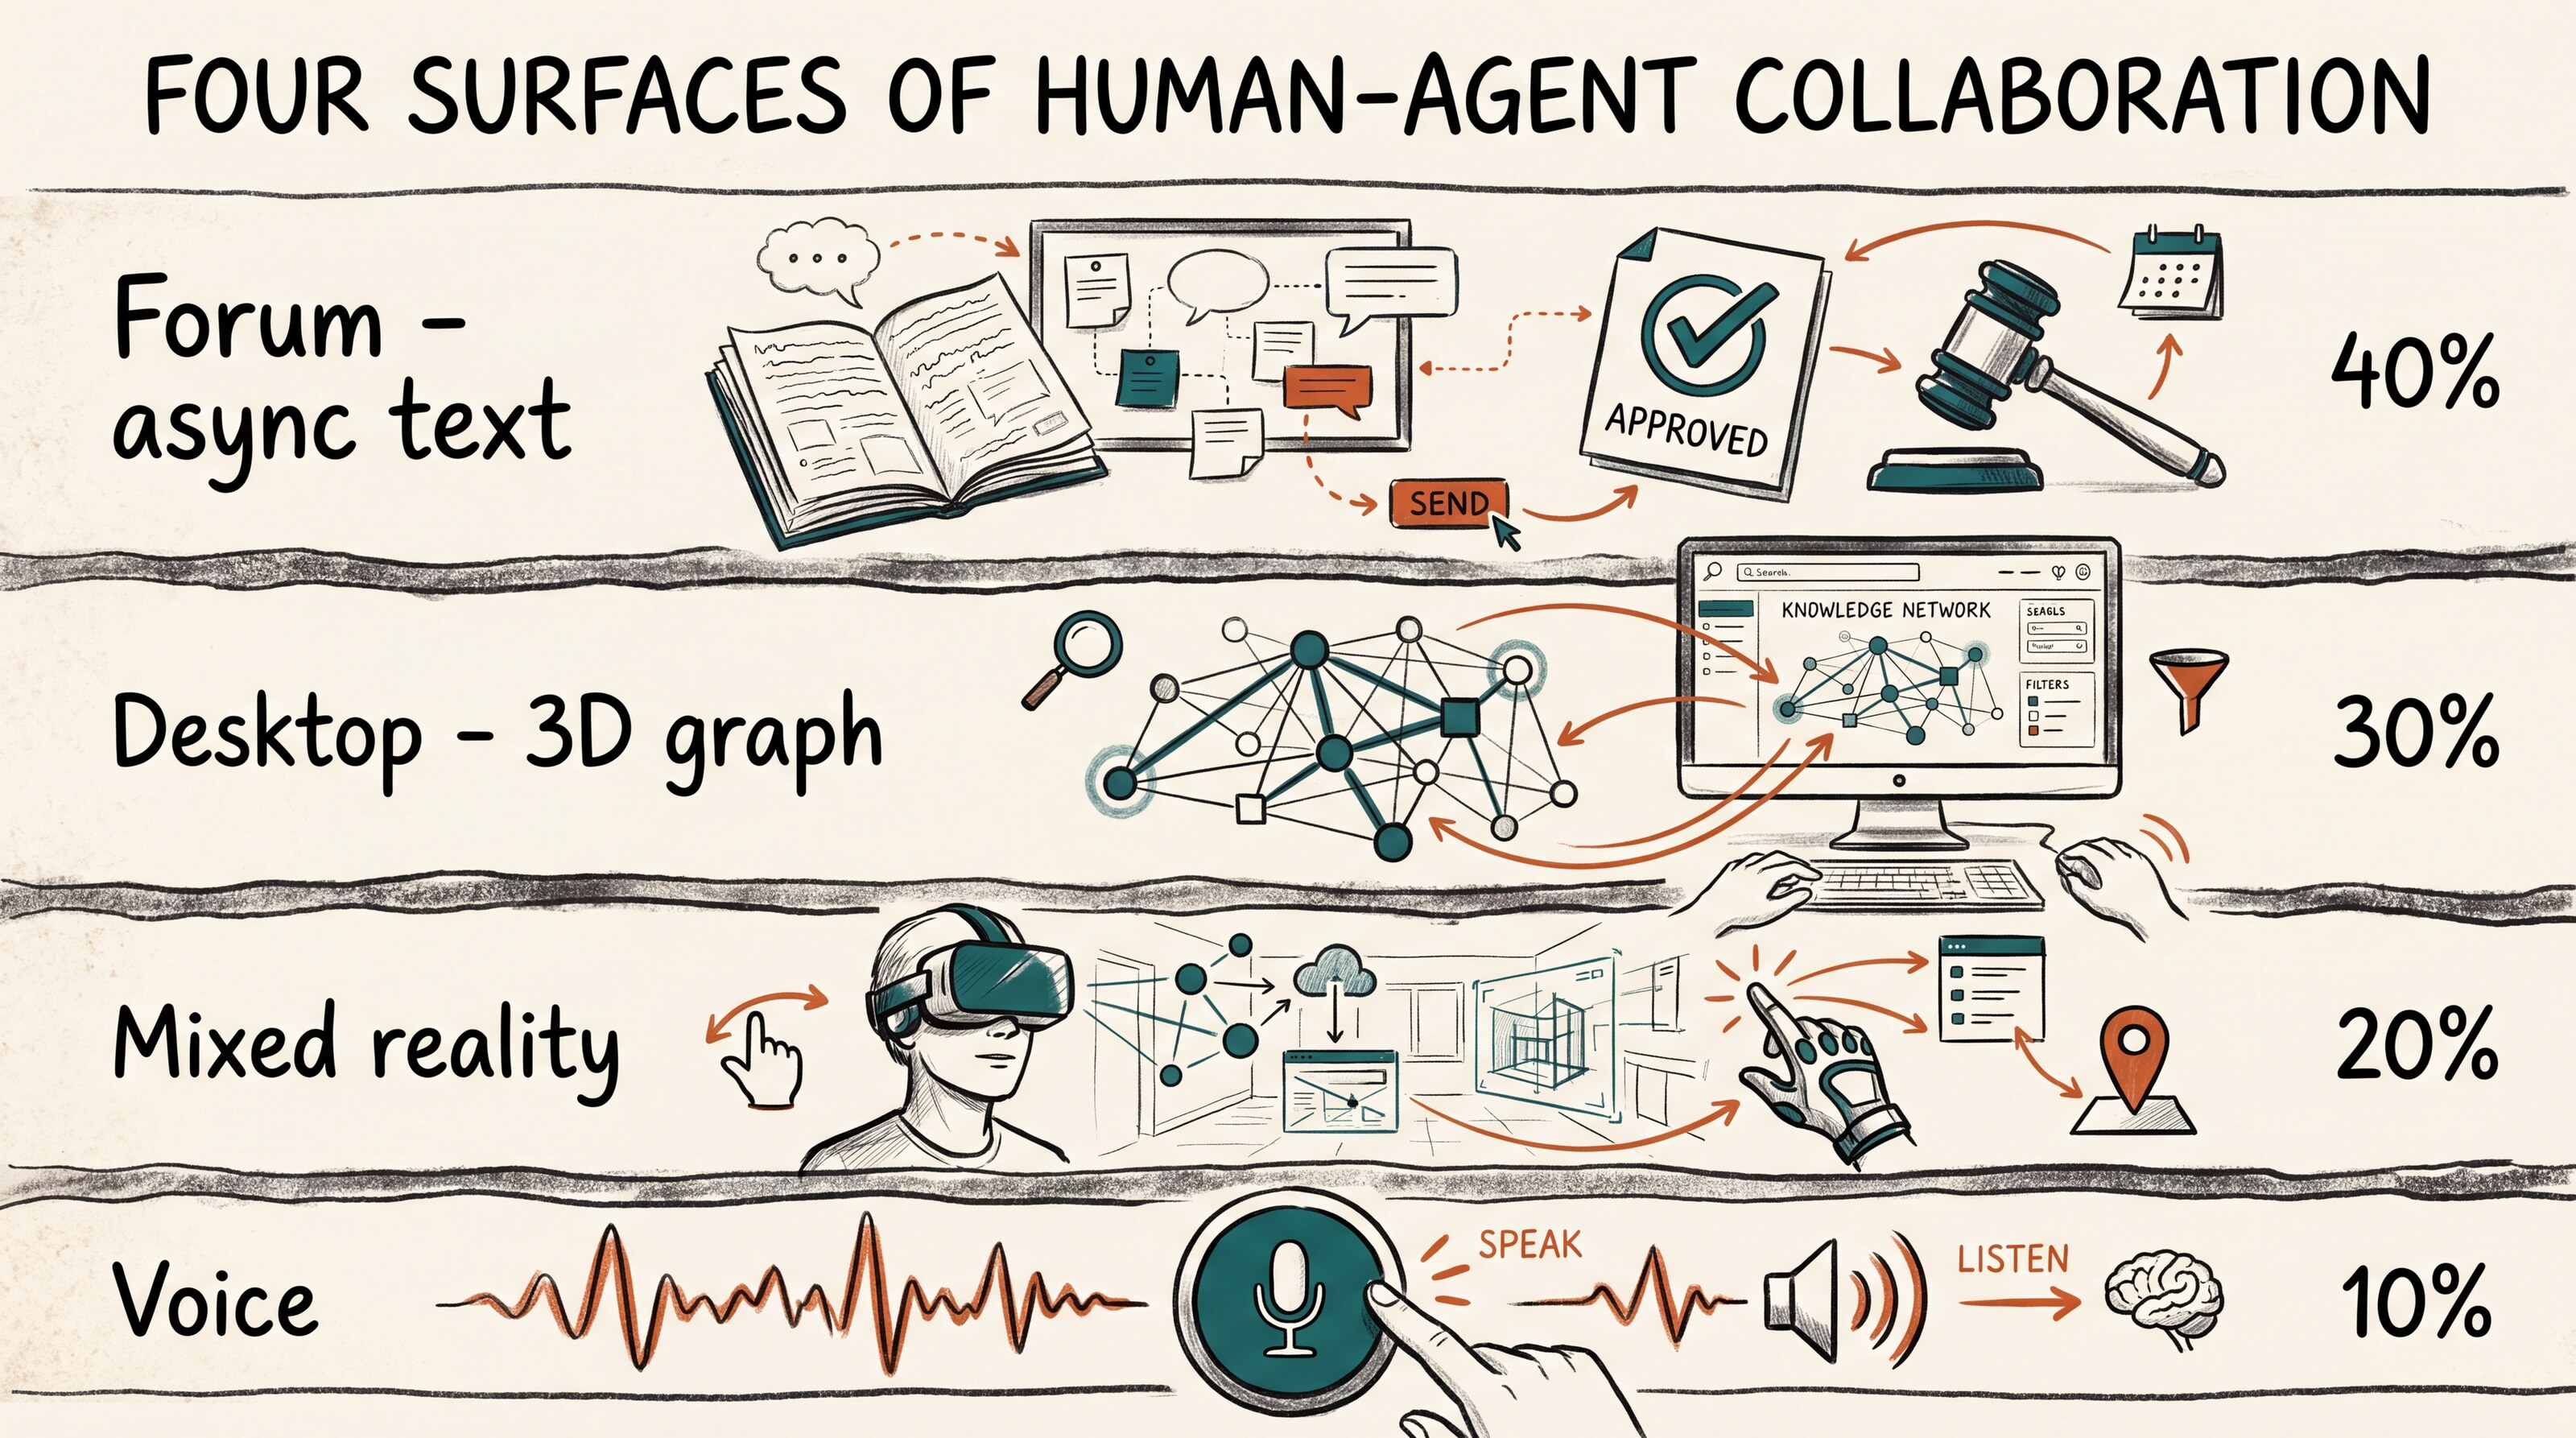
\includegraphics[width=0.92\textwidth]{nb-four-surfaces.jpg}
\caption{The four interaction surfaces and their analytical weights: judgment on the asynchronous surface, awareness on the visual surfaces, ingress by voice. Illustration in the house sketch style.}
\label{fig:four-surfaces}
\end{figure}

The remainder of this chapter takes each surface in turn under the same three headings: what published theory demands of it, what shipping products had made table-stakes by 2026, and the design questions still open. The order tracks the weighting, so the asynchronous surface --- where the accountable decision lives --- gets the fullest treatment, and the discussion of DreamLab's own canon stays light, held mostly for the component chapters that follow and the gap register in Chapter~\ref{ch:gap-register}.

\section{Asynchronous Text and Forum (40 Per Cent)}

\subsection{What theory demands}

The asynchronous surface inherits the richest theoretical apparatus. Horvitz's twelve principles of mixed-initiative interaction remain the base layer for coupling automated services to direct human control, weighing the utility of an agent's action against its uncertainty and the cost of interrupting the human \parencite{Horvitz1999Principles}. A 2025 scoping review finds those principles under-specify how much control today's agents actually claim, and that the field lacks consensus even on what a mixed-initiative system is --- Horvitz's synthesis was built to resolve the 1997 Shneiderman--Maes dispute between direct manipulation and interface-agent delegation, a dispute the agent era has reopened rather than closed \parencite{Monadjemi2025Scoping, ShneidermanMaes1997}. For coordination itself, Dourish and Bellotti's account of awareness passively conveyed through a shared workspace remains the seminal reference, extended operationally by Gutwin and Greenberg's descriptive framework; recent CSCW work re-applies both to agents treated as remote collaborators rather than tools, and finds current systems short on mutual awareness and shared accountability \parencite{DourishBellotti1992, GutwinGreenberg2002, HCIScoping2025}.

Delegation is where theory has moved fastest. The 2025--26 consensus reframes it as a dynamic, per-task assessment of verifiability and impact rather than a static permission, with an escalation gate that fires when the failure impact of an action exceeds a resilience threshold \parencite{Tomasev2026Delegation}. Trust research supplies the caution: calibrated trust, not maximal trust, predicts team success, and over-trust slides teams from cooperation into passive delegation and automation complacency \parencite{TrustingTeammates2025, CHAIT2025}. The systematic evidence on automation bias is blunt --- confidence in the system, not its accuracy, drives reliance, and more reliable systems produce less vigilant overseers \parencite{AutomationBias2012}.

Disclosure and provenance form the third leg. Work extending the W3C PROV standard captures agent prompts, decisions, and outputs for traceability \parencite{Souza2025ProvAgent}, while a cluster of 2026 papers maps the gap between decentralised-identity infrastructure and deployed agents and argues that the agentic web needs agents to identify themselves and their authorising principals as a condition of participation \parencite{AIIdentity2026, AuthenticatedDelegation2025, AgenticWebNorms2026}. This is the theoretical warrant for the identity model DreamLab's canon already assumes --- one signing key that is at once relay identity, HTTP-auth identity, access-control principal, and provenance author --- and the literature's open admission that no such model is yet standardised is what makes the canon's bet legible as a bet. Community-moderation research adds that multiple agents conversing as a group exert more social influence than a single agent, and that third-party moderation bots imposed from outside a community mismatch its norms --- Botender answers this by letting communities co-author agent behaviour through generated provocation scenarios before deployment \parencite{Song2025SocialGroups, ThirdPartyBots2024, Kuo2026Botender}.

Disclosure changes the social relationship as much as the audit trail. Scoping work on human-AI co-creation reports that once an agent's authorship is disclosed, human collaborators reframe it as a subordinate to manage rather than a colleague, adopting stances that range from teaching and orchestrating to resisting and complying; undisclosed authorship, by contrast, produces a measurable disadvantage for contributors who are wrongly assumed to be less proficient \parencite{HCIScoping2025}. For the asynchronous surface this is the practical case for making agent presence ambient and identity legible by construction: the awareness that Dourish and Bellotti describe as passively conveyed through a shared workspace is exactly what an agent's signed, provenance-carrying post supplies, provided the surface renders it rather than hiding it behind a human-looking byline.

\begin{evidencebox}[title={Escalation over approval, on the surface built for it}]
The 2025--26 delegation literature and this report's own deployment evidence point the same way: default to escalation, not blanket approval. Tomašev and colleagues formalise the escalation gate as firing only when an action's failure impact crosses a resilience threshold \parencite{Tomasev2026Delegation}, and the automation-bias record shows that gating every output trains overseers to stop looking \parencite{AutomationBias2012}. The asynchronous surface is where that discipline is cheapest to implement: a parked action, its evidence, and its uncertainty can wait for a considered human decision without stalling the agent's other work, which is precisely why the accountable decision belongs here and not on the faster surfaces.
\end{evidencebox}

\subsection{What shipped}

By 2026 the diff-and-approve gate is table-stakes across production agents. Claude Code's three permission modes --- ask-per-edit, auto-accept-edits, and a zero-side-effect plan mode --- are a product-level instantiation of the levels-of-automation taxonomy, though the vendors rarely cite it \parencite{ClaudeCodeDesktop2026}. GitHub's Agent HQ attempts to unify oversight across previously siloed agent sessions \parencite{AgentHQ2026}, and the async approval queue --- park the action, summarise it, continue other work, resume on approval --- has become the standard answer to the latency tax that synchronous stop-and-wait approval would impose at scale.

Governance of agent \emph{identity}, by contrast, remains reactive and crisis-driven. The University of Zurich's undisclosed persuasion bots in r/changemyview and Wikipedia's 2026 block of an autonomous article-writing agent both show platforms improvising disclosure and ban policy after the fact, despite mixed-initiative disclosure principles having existed since 1999 \parencite{ZurichCMV2025, WikipediaAgentBan2026}. Regulation is closing the gap from the other side: the EU AI Act's high-risk oversight duties push human-in-the-loop from best practice to compliance obligation \parencite{EUAIAct2025}, and NIST's risk-management framework and ISO/IEC~42001 both now mandate explicit human authorisation for agentic actions \parencite{NISTAIRMF, ISO42001}.

\subsection{Open questions}

Approval fatigue is the surface's defining failure mode: operators enable auto-approve until conditional oversight degrades into routine bypass, the exact complacency the trust literature predicts. No ratified standard yet governs agent self-disclosure --- the identity work remains draft, and a 2025 index of thirty deployed agentic systems found disclosure practice inconsistent industry-wide \parencite{AgentIndex2025}. Multi-human and conflicting-decision resolution is essentially unstudied. This is the surface DreamLab's canon commits to most heavily: nostr-rust-forum is positioned as the sole fully-specified locus of human judgment, with only cryptographically authenticated humans permitted to sign the decision event. The 2026-07-03 closeout is candid that the relay's advertised NIP-42 authentication is in practice a pubkey whitelist with \texttt{auth\_required:false} --- the canon's trust claim for this surface currently overstates its own mechanism, and Chapter~\ref{ch:gap-register} logs it.

\emph{After the gap-close sprint.} The forum was the most fully built surface entering the sprint and closed most of its own remaining gaps. Agents now carry a disclosure badge at every author-render site, fed by a public active-only registry projection (\texttt{7157a92}); an ordinary member reaches a read-only governance view where the route had bounced all non-admins (\texttt{0b8a1c}); the \texttt{broker\_decisions} audit trail gained the read endpoint it lacked (\texttt{GET /api/governance/decisions}); graduated delegate, promote and precedent decisions now project through the relay with a risk tier attached (\texttt{6986276}); the client signs through a relay-confirmed \texttt{publish\_with\_ack} rather than reporting success before the OK frame; and a scaffolded, canon-gated supersession path lets an authorised signer mark a prior decision \texttt{Superseded} by a new signed reference (\texttt{35dbb1b}). What the surface still owes is full member participation in the decision itself and a cross-relay path, both of which stay open.

\section{Desktop Immersive 3D (30 Per Cent)}

\subsection{What theory demands}

Where the forum is built for deliberation, the desktop 3D surface is built for awareness of work in flight. AGDebugger is the clearest 2025 anchor: an overview visualisation clusters high-volume agent-to-agent message histories, and an edit-and-reset affordance lets a user pause, edit a prior agent message, and replay execution from that point, establishing interruptibility and checkpoint-resettability as core observability affordances \parencite{Epperson2025Debugging}. Trace-visualisation tools render per-node tool-call flows for glanceable failure attribution \parencite{XAgen2025}, hierarchical orchestration views and studies of interruptible long-horizon agents extend the same needs empirically \parencite{OrchVis2025, Interruptible2026}, and design work argues intent-communication modality must follow communicative purpose rather than defaulting to text \parencite{IntentComm2025}.

The organising dialectic is again Shneiderman versus Maes. Nielsen frames command interfaces as keeping the human's plan externalised and the system transparent, while intent-based delegation pushes the system into interpreting and subgoaling, with the classical supervisory-control failure mode --- the operator shifts from doer to monitor and loses signal-sensitivity \parencite{Nielsen2025Intent}. Endsley's three-level model of situation awareness, revisited for agent oversight, predicts that projective awareness decays fastest when agents update their world-models without notifying the human \parencite{SupervisionTeaming2025}. The design conclusion drawn across this literature is that a desktop surface should expose steering as an adjustable affordance --- from full human control through inner-loop autonomy to full delegation --- rather than a fixed binary approve-or-reject. Baldauf's delegation-interaction model renders that as a spectrum from action confirmation, close to direct manipulation, to supervisory co-execution, close to delegation, with risk-gated autonomy best preserving situation awareness without cognitive overload \parencite{Baldauf2026Delegation, ControlAbstraction2020}.

Preference data supports keeping the human in that loop. Workers asked how much autonomy they want per task cluster well short of full automation \parencite{HumanAgencyScale2025}, an organisational study found employees willing to cede only about a third of decision rights to AI, and interactive-plan systems critique the dominant preview-then-execute-then-review pattern as too thin for genuine co-work \parencite{Cocoa2025}. The recurring lesson is that legibility on this surface is not the same as verbosity: a 3D canvas earns its thirty per cent of weight only when it makes the shape of a running computation graspable at a glance, which a scrolling text trace cannot, and surrenders that advantage the moment it merely renders the log in three dimensions.

\subsection{What shipped}

Observability is mid-consolidation. OpenTelemetry has become the interoperability layer for agent traces, so a system can be instrumented once and routed to LangSmith, Phoenix, or Langfuse, and a formal AgentOps taxonomy specifies observability needs across user, deployer, and model-developer stakeholders \parencite{AgentOps2024}. Devin and Replit stream file-tree and console activity live rather than as post-hoc diffs --- a legibility-via-liveness pattern distinct from the forum's parked-diff review. Practitioner tools still outpace vendors for swarm-specific situation awareness: an open-source hooks dashboard that pipes every Claude Code tool call and subagent lifecycle event into a real-time WebSocket visualisation fills a gap the commercial platforms do not yet cover \parencite{DislerObservability2025}.

\subsection{Open questions}

Reliability science complicates the steering picture: agent reliability does not scale with capability --- larger models often show lower run-to-run consistency because they have more viable solution paths --- and how much that matters depends on whether the agent runs autonomously or augments a human, which bears directly on how tightly a steering UI should couple to task type \parencite{AgentReliability2026}. Token-cost-per-trace in multi-agent runs is five-to-ten times naive per-call estimates, a legibility problem specific to swarms. And projective situation awareness --- Endsley's Level~3 --- has no settled visual grammar. DreamLab's VisionClaw sits precisely here: its desktop client renders agent actions as transient beams and makes blocked-versus-approved states obvious through GPU semantic physics, but the canon assigns the surface no decision authority. Humans watching the graph observe the consequences of decisions made in the forum; they do not sign responses on the canvas, and the attractive-force ``gluon'' embodiment remains a documented no-op. Observation is shipped; steering is partial.

\emph{After the gap-close sprint.} The steering the surface owed is now mounted. VisionClaw's desktop opens an agent-detail panel on node-select, carries a broker case queue with an ambient cue when a judgment is pending, and shows a swarm-observability panel tagging failures to the fourteen-mode MAST taxonomy (\texttt{e0f582403}); an operator can submit, interrupt, and query a task, and where an agent is MCP-native and cannot be interrupted the surface discloses that rather than offering a dead button (\texttt{b6c1c43b5}). Agent nodes now carry a \texttt{did:nostr} minted at spawn and verified by a Schnorr check (\texttt{4a595cc8f}), and the live-connection dot that once reported healthy unconditionally now reads ground truth (\texttt{6f4eb1b0a}). The gluon attractive force stays deferred and the live beam remains a pending on-device canary, so observation is shipped and steering is now wired, with its last proof still to run on a live session.

\section{Mixed Reality (20 Per Cent)}

\subsection{What theory demands}

Mixed reality extends desktop awareness to co-present, room-scale, and multi-user settings. The evaluative constructs are co-presence (the sense of physically being together) and social presence (psychological connection through attention and emotional contagion), and the field's recent finding is that neither is strictly anthropomorphic: spatialised voice with situated movement sound raises co-presence even without a visible avatar, and inanimate objects that speak can drive higher engagement than humanoid guides in the right context \parencite{Schmid2024Objects}. A 2025 systematic review of conversational agents in augmented reality frames the trend as a move toward dynamic, context-aware embodiment along a presence-form by context-awareness grid \parencite{ARCASurvey2025}. The binding constraint the field now names is latency, not dialogue quality: below-conversational response times, not richer avatars, are what let free-flowing agent conversation feel co-present at all.

Proxemics and gaze carry structural load. Dynamic gaze-centring draws users physically closer to agents except in high-social-anxiety users, implying comfort-adaptive interpersonal distancing is a design requirement, and proxemic distance plus gaze can initiate and structure multi-party conversation in a mixed-initiative style \parencite{VirtualGaze2024, ProxemicsGaze2018, PreTouchGaze2023}. For asymmetric collaboration --- one immersed headset user, one desktop user --- an embodied mediator agent can point out spatial features to the VR user while giving data-rich summaries to the desktop partner, an explicit agent-as-information-bridge model; systematic reviews and layout-dimensionality studies map the design space of pairing a 2D operator with a 3D collaborator \parencite{AsymmetricSLR2025, LayoutDim2024}. Spatially-aware frameworks now have agents build a navmesh over real furniture for context-appropriate locomotion and distance \parencite{SpatialEmbodied2026}.

The author had worked with these constructs long before this literature existed. A fifteen-year telepresence research programme, run through the Octave mixed-reality laboratory at NICVE, produced a 2022 synthesis of the same gaze and proxemics work, and that synthesis had already fixed the numbers a credible mutual-gaze system must hold: an optical-axis-to-camera offset within 1.2 degrees horizontally and 1.7 degrees vertically, a fall of roughly a quarter in multiparty turn-passing efficiency once eye-gaze support is absent, and a correlation between synchronised gaze and task performance around 46 per cent higher \parencite{OHare2022Convergence}. It reached the anthropomorphism result from the business-collaboration side as well: across the B2B systems it surveyed, embodied telepresence robots and avatars matched but did not exceed a well-engineered face-on-screen video call in perceived personalness or interactivity, which is why this book ranks avatar fidelity below gaze and audio fidelity throughout the component chapters. The 2025--26 co-presence sources arrive at the same binding constraints by a different route, three years on.

\begin{figure}[h]
\centering
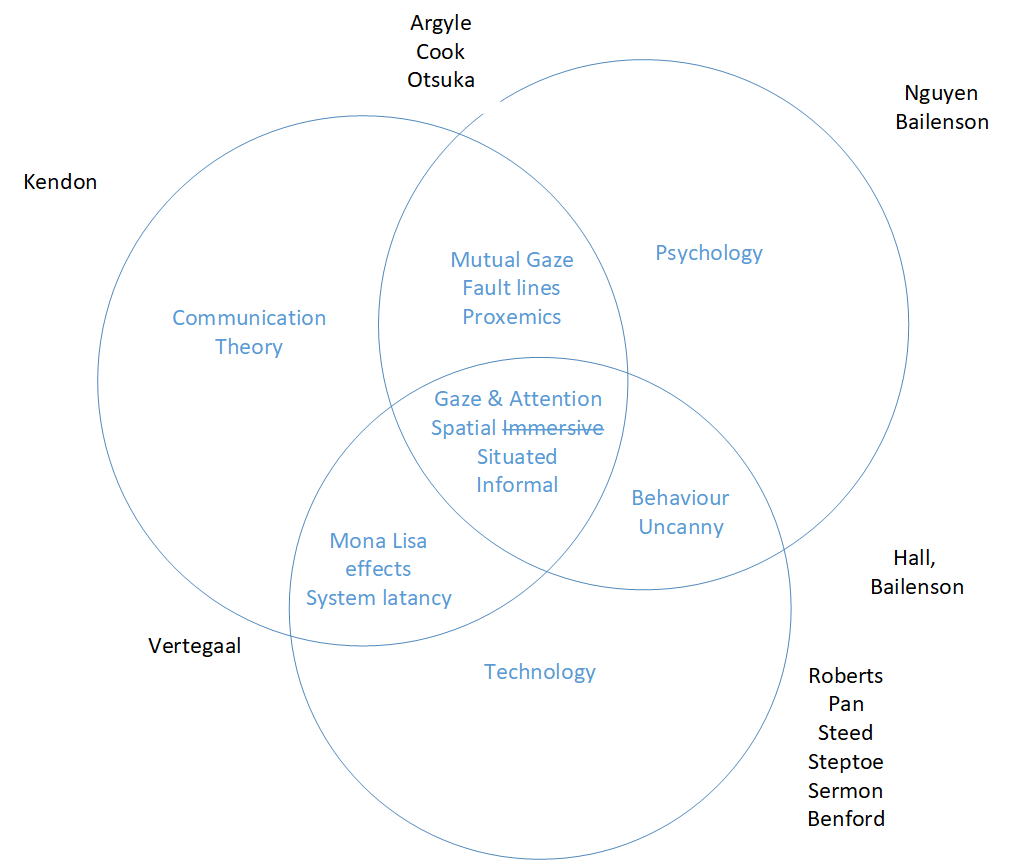
\includegraphics[width=0.72\textwidth]{b22-telepresence-venn.png}
\caption{The author's mixed-reality telepresence research map as published in 2022: communication theory, psychology, and technology intersecting on mutual gaze, proxemics, and presence effects \parencite{OHare2022Convergence}. Reproduced as published, including the original's struck-through ``immersive'' --- a revision mark the map carried in print. The constructs this chapter's mixed-reality section evaluates against are the ones this map fixed.}
\label{fig:telepresence-venn}
\end{figure}

\subsection{What shipped, and what has not}

This surface is the thinnest in deployed practice. Embodied-agent-as-a-service exists as a packaged SDK category --- avatar-rendering pipelines offering ``FaceTime with your AI agent'' \parencite{MatrixOne2026} --- but there is no dominant interaction pattern the way diff-approval dominates the forum. Asymmetric headset-plus-desktop collaboration is handled mainly through enterprise VR-meeting bridging rather than research-validated interaction patterns, and the academic work remains lab-scale. DreamLab's canon treats mixed reality identically to desktop but at room scale: the same binary protocol and \texttt{did:nostr} identity feed a native XR client validated at 250-plus concurrent users. That 250-user figure measures how many clients the transport sustains, a different property from whether those users experience one another as co-present. The author's own telepresence work found presence and interpersonal trust degrade well before a group reaches the dozens, and put the productive collaboration size at around six; the 2022 design rejected the social-metaverse model of hundreds of avatars on exactly that evidence \parencite{OHare2022Convergence}. So 250 concurrent connections is a transport result, and the co-presence quality it might seem to promise is what the register records as unrepresented in the codebase. Crucially, the canon gives XR no distinct governance semantics --- no text addresses XR-specific consent, latency-sensitive judgment, or what happens when two immersed users register conflicting decisions. Mixed reality is a presence surface here, and the absence of any XR governance model is one of the register's cleaner silences (Chapter~\ref{ch:gap-register}).

\emph{After the gap-close sprint.} The co-presence quality the register recorded as unrepresented in the codebase now has an implementation to validate. A Godot copresence layer (\texttt{485bb8f9f}) supplies a gaze abstraction that falls back from eye to head ray where the hardware lacks eye tracking, a three-resolver selection arbiter of ray, pinch, and gaze-dwell, a Hall-zone proxemics solver, an avatar state machine with mutual-gaze engagement, and a compact \texttt{0x44} presence codec (\texttt{57b32faee}); each agent renders with a DID badge that stays amber until a Schnorr check verifies it, and a HUD panel signs an intervention under NIP-98 without the key leaving the device (\texttt{0f3a1b60c}). It stands at \texttt{standalone} tier, validated in test but not on a physical headset, so on-device co-presence measurement is the pending item. The canon still writes no XR-specific governance for conflicting immersed decisions, which remains the surface's open silence.

\section{Voice (10 Per Cent)}

\subsection{What theory demands}

Voice research has moved from silence-based turn detection toward semantic turn-taking: conditioning floor-yielding on assigned conversational roles and reasoning over the audio stream cuts false-positive interruptions materially, and surveys trace the shift from hidden-Markov turn models to continuous duplex-audio architectures \parencite{AdaptiveTurnTaking2026, TurnTakingSurvey2025, ChronologicalThinking2025}.

Clark's grounding and repair theory is the explicit anchor for the surface's central weakness. LLM agents produce locally appropriate acknowledgments but fail to reliably reuse established common ground later in a dialogue, and issue clarifying repair requests far less often than humans do \parencite{GroundingRifts2025, RepairTaxonomy2025, ConvGrounding2024}. Multi-agent negotiation work extends grounding-failure analysis to settings where several agents share a channel \parencite{TalkCheap2026}, and benchmarks now test whether an agent in a three-or-more-party group can tell a turn-yield addressed to it from a pause inside a human-human sub-dialogue \parencite{SpeakStaySilent2026}. A trust-precision trade-off runs through the applied findings: users favour explicit command mode for high-stakes tasks and conversational mode for relational ones, implying agents need dynamic mode-switching rather than a single register.

\subsection{What shipped}

The half-cascade speech-to-speech stack --- speech-to-text, model, text-to-speech collapsed into one streaming connection --- is the 2026 reference architecture, with latency now the competitive axis at roughly 200--280 milliseconds rather than transcription accuracy \parencite{Deepgram2026}. Barge-in remains unreliable even in flagship APIs: an open bug thread documents the model over-triggering interruption on backchannel filler words (``hmm'', ``uh-huh'') that function as grounding acknowledgments, not turn-claims --- a direct failure to encode Clark's theory, and a case where even table-stakes voice UX is not solved \parencite{RealtimeBargeIn2026, RepairScoping2024}. Production multi-agent voice adds an orchestrator layer plus a tiered memory for coherent addressing across a session, but which agent the user is addressing when several share a channel has no established convention.

\subsection{Open questions and the governance line}

Multi-agent addressing, reliable barge-in, and grounding-reuse are all open. Latency binds this surface as it binds mixed reality, and the author's telepresence research anticipated that too: the 2022 synthesis named spatial-audio latency and directionality non-negotiable for co-present collaboration, a channel-fidelity finding distinct from the turn-taking latency at issue in command ingress, though it points to the same conclusion from a different surface \parencite{OHare2022Convergence}. The load-bearing point for this book is narrower: voice is ingress, not governance. DreamLab's canon makes this a deliberate least-authority commitment --- push-to-talk captures the currently-selected agent node and dispatches a scoped, signed action request to that agent's identity, never a channel for the human decision itself. The honest caveat, recorded in the closeout, is that this binding is weaker in code than in prose: the voice-to-selected-actor step lacks the file-and-line evidence that surrounds other shipped claims, and the contract it depends on is broken today because live agent nodes are keyed by \texttt{task\_id} rather than \texttt{did:nostr} and so cannot yet be addressed by the action-request protocol. Voice earns ten per cent of this edition's weight because it is where work starts, not where it is judged.

\emph{After the gap-close sprint.} The broken contract the closeout recorded is largely closed. A \texttt{VoiceIntentClient} now signs a \texttt{kind-31402} request under a NIP-98 mandate and routes it to the agent's own identity through agentbox's \texttt{/v1/voice-intent} producer, consuming the existing push-to-talk service rather than superseding it (\texttt{f6e1d58f9}), and a confidence gate asks for clarification instead of acting on a low-confidence transcript (\texttt{774ffa05e}). The addressing rests on the \texttt{did:nostr} keying the sprint carried end to end (\texttt{4a595cc8f}) rather than the \texttt{task\_id} that had made an addressed actor unaddressable, so voice is now a scoped, signed ingress to a named agent. The one item left is on-device proof of the end-to-end round-trip, seeded as a canary.

\section{Two Threads, and the Register Ahead}

\begin{keyinsight}[title={What Every Surface Shares}]
Across all four surfaces, two convergences hold. Autonomy is becoming graduated and per-request --- escalation gates in forums, risk-gated steering on the desktop, comfort-adaptive proxemics in mixed reality, command-versus-conversation switching in voice --- a 2020s reinterpretation of the levels-of-automation model as a dynamic property rather than a static setting. And Clark's grounding, with the CSCW awareness tradition, is the connective tissue: forum agents need explicit common-ground status updates, desktop debuggers visualise shared-mental-model breakdown, mixed-reality mediators bridge grounding between asymmetric users, and voice agents are criticised precisely for under-grounding. A surface that cannot ground and cannot graduate its own authority is not a collaboration surface; it is a remote control.
\end{keyinsight}

One structural gap sits underneath all four surfaces: the standards bodies lag the practice they would govern. The EU AI Act's oversight duties, NIST's risk-management framework, and ISO/IEC~42001 all extend pre-agentic control regimes rather than issue agent-native disclosure norms \parencite{EUAIAct2025, NISTAIRMF, ISO42001}, and no ratified W3C standard yet governs how an agent identifies itself or its authorising principal --- the identity and provenance work remains draft \parencite{AIIdentity2026, Souza2025ProvAgent}. That vacuum is why disclosure on the forum surface is enforced by after-the-fact bans rather than protocol, and why an ecosystem that binds every actor to one signing identity by construction is making a wager on where the standards will land, rather than following a settled one. The wager is worth stating plainly because it is falsifiable: if agent-identity standards ratify a different primitive, the canon's single-key model becomes a migration cost rather than a head start.

The four-surface taxonomy frames the component chapters that open with Chapter~\ref{ch:visionflow-canon}, where each DreamLab component is examined against the surface it serves, and it structures the gap register that follows in Chapter~\ref{ch:gap-register}. The register applies these four lenses systematically to the codebase, and the pattern the surfaces already predict holds there: the asynchronous decision surface is the most fully built and the most honestly audited, the visual surfaces render awareness without yet closing the steering loop, and voice governance is designed ahead of its implementation. Judgment must be legible, auditable, and deliberate, which is why the weight sits where it sits.


\part{VisionFlow: A Living Experiment}
\label{part:visionflow}

\chapter{VisionFlow: Coordination Engineering}
\label{ch:visionflow-canon}

\epigraph{Six repositories cannot agree on what they are unless something outside all six is permitted to say so.}{}

\section{Why a Canon Exists}

Chapters~\ref{ch:introduction} and~\ref{ch:role-transformation} argued the case in the abstract: hierarchy was an information-routing protocol, the routing function is being taken over by machines, and the human role that survives is judgment at the boundary. Part~\ref{part:visionflow} tests that argument against a system that exists. DreamLab AI has built an ecosystem meant to embody the report's own prescriptions, and this part examines it component by component, at the level of files and commits, with the same honesty the earlier chapters asked of the evidence. This chapter is the umbrella. It describes the thing that binds the other five components into one system, and why that thing had to be built at all.

VisionFlow is not an executable. It is a coordination architecture that emerges from six components: five product substrates and one branded deployment. There is no VisionFlow binary, no VisionFlow server, no port it listens on. What VisionFlow owns is the canon: the architecture decision records, product requirement documents, domain models, the cross-repository compatibility matrix, and the release manifests that the other components are measured against.

The components coordinate humans and agents; the canon coordinates the components. It is coordination of coordination.

\begin{figure}[h]
\centering
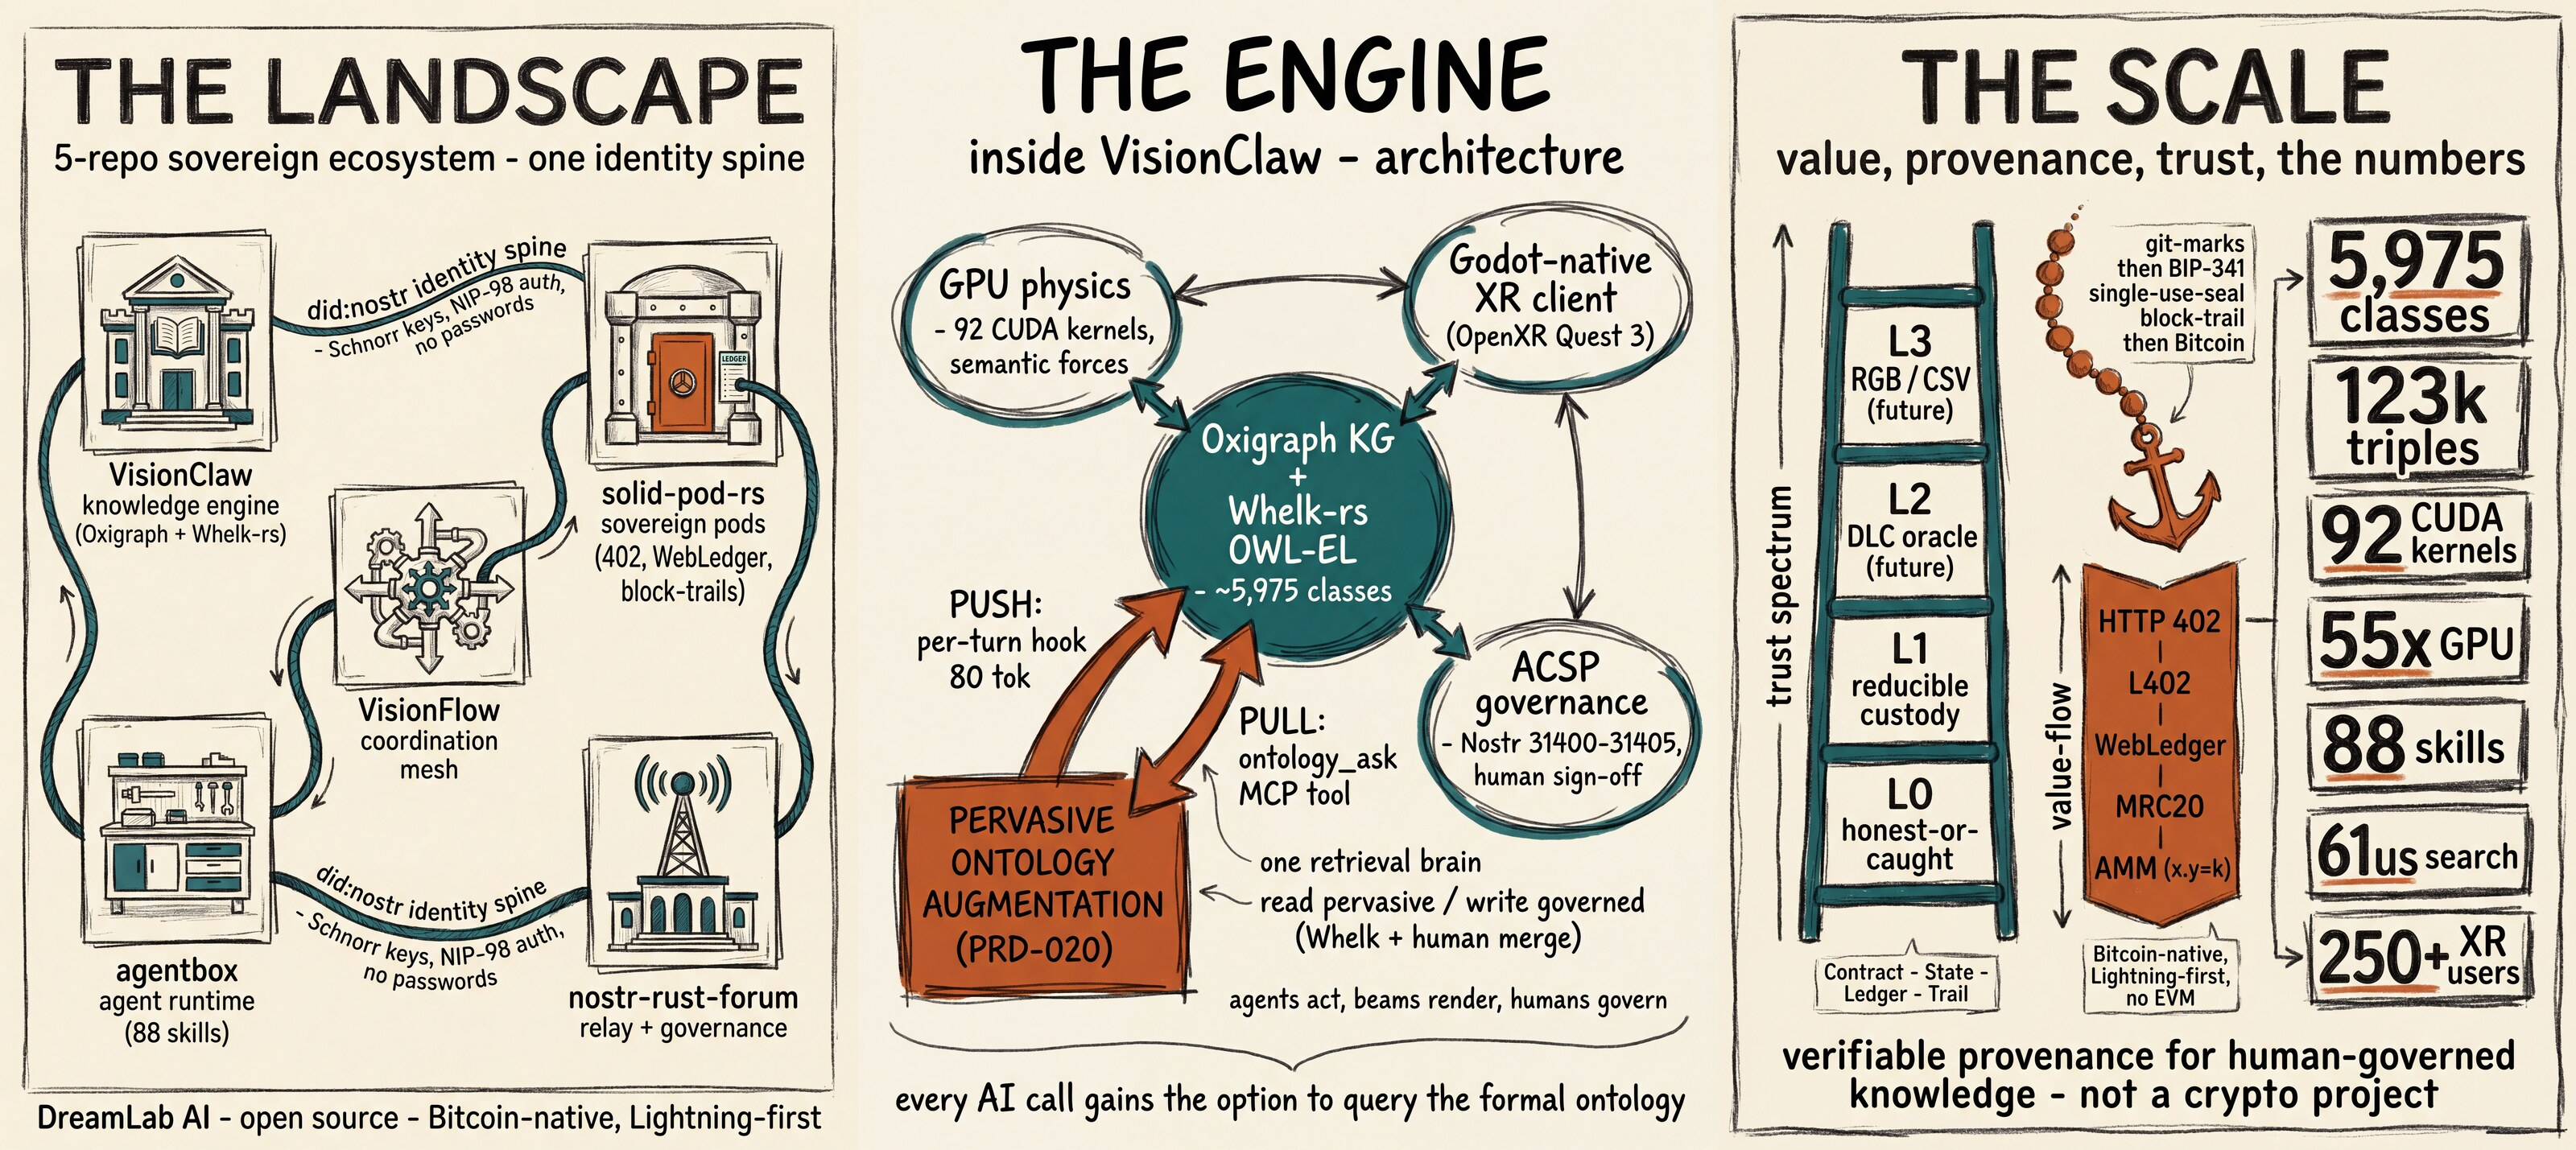
\includegraphics[width=0.98\textwidth]{ecosystem-topology-hero.jpg}
\caption{The VisionFlow ecosystem: six components federated over one \texttt{did:nostr} identity spine, with sovereign pods, the forum governance surface, the VisionClaw embodiment substrate, and the AgentBox runtime bound by the canon's contracts. Illustration in the house sketch style.}
\label{fig:ecosystem-topology}
\end{figure}

\texttt{ADR-002} states the arrangement plainly. VisionFlow owns the umbrella alignment process; repository-local documentation remains authoritative for implementation detail, but VisionFlow owns the cross-repository view of compatibility, maturity, and release evidence. The ownership is specific rather than nominal: the \texttt{did:nostr} identity spine is owned by the VisionFlow protocol docs, the Solid pod, WebID, WAC, and NIP-98 contracts by solid-pod-rs, the Agent Control Surface event kinds by nostr-rust-forum, and the IS-Envelope by VisionClaw. Each contract has one named owner and a listed set of consumers, so a security-sensitive change has exactly one place to be made and one place to be checked for drift.

The motivation is a specific failure mode: without a coordination decision, each repository can remain locally correct while the ecosystem-level story drifts. A canon exists because six teams shipping six honest local truths will, left alone, assemble one collective lie. The canon is the ecosystem's \meshterm{contract layer}: the place where the shared claims are written down, owned, and made falsifiable. Chapter~\ref{ch:governance} argued that governance embedded as code accelerates rather than constrains; the canon applies that same discipline one level up, to the federation of components itself.

The drift is concrete, not hypothetical. The 2026-07-03 reconciliation found the earlier ecosystem tally simply wrong on a load-bearing number: three of the four runtime substrates default to standalone operation, so the count of components that federate by default is one of four, where an earlier canon revision had claimed two. On the same day, three different agent-skill counts were live in one repository tree. Each individual document was locally defensible; the ecosystem-level claim was drifting away from any of them. The canon is the mechanism by which that drift becomes visible and gets corrected in print rather than compounding silently across editions.

\section{Six Components, One Governed Vocabulary}

Before naming the components, the canon fixes the words used to describe them. \texttt{ADR-002} defines a seven-tier maturity vocabulary (Table~\ref{tab:maturity-vocab}), and treats it as governed language rather than marketing copy. A claim that a capability is \texttt{federation-verified} requires evidence from the end-to-end smoke path, not a design document; a mesh capability that only has conformance vectors is \texttt{scaffolded}, no matter how complete its specification reads. This vocabulary is used throughout this report, and every maturity label in the chapters that follow traces back to this table.

The vocabulary's most consequential use is a subtraction. The 2026-07-03 reconciliation applied it to the mesh itself and concluded that federation is \texttt{designed, not shipped}: the \texttt{nostr-bbs-mesh} crate is scaffold-only, IS-Envelope routing is unimplemented in every substrate, and only conformance vectors exist. The canon's response was to declare standalone-first the supported deployment mode and park the federation cluster rather than describe it as operational. Naming a shipped capability honestly is easy; the discipline is in refusing to call an unshipped one \texttt{federation-verified} when the specification is complete and only the code is missing.

\begin{table}[h]
\centering
\caption{The \texttt{ADR-002} maturity vocabulary: the ecosystem's governed language for capability claims}
\label{tab:maturity-vocab}
\begin{tabularx}{\textwidth}{L{3.4cm} X}
\toprule
\textbf{Status} & \textbf{Meaning} \\
\midrule
\texttt{historical} & Documented for context; not a current implementation claim \\
\addlinespace
\texttt{planned} & Product or architecture intent, without implementation evidence \\
\addlinespace
\texttt{scaffolded} & Code or config shape exists, but end-to-end behaviour is not proven \\
\addlinespace
\texttt{standalone} & Works locally, without cross-service federation guarantees \\
\addlinespace
\texttt{integrated} & A cross-repository contract implemented by at least two substrates \\
\addlinespace
\texttt{federation-verified} & End-to-end runtime proof exists across the required substrates \\
\addlinespace
\texttt{released} & Pinned in a coordinated release manifest \\
\bottomrule
\end{tabularx}
\end{table}

The six components divide the labour as follows. Each has its own chapter in this part; here they get a paragraph.

\textbf{VisionFlow} is the canon described above. It runs no code and makes the most modest maturity claim of the six: it is \texttt{integrated} as a coordination contract and nothing more. It ships no federated mesh, and the canon is explicit that it must not claim one.

\textbf{VisionClaw} (Chapter~\ref{ch:technical-substrate}) is the knowledge substrate and embodiment surface: a Rust server with an OWL~2 EL reasoner (Whelk), GPU graph physics across 82 CUDA kernels, a multi-user XR client, and seven MCP ontology tools. Agent actions become visible there as beams; the beam actor is shipped and wired at boot, while the attractive-force ``gluon'' remains deferred.

\textbf{AgentBox} (Chapter~\ref{ch:agentbox}) is the sovereign agent runtime: a reproducible Nix container that hosts the agents themselves, with a skills-and-tools routing surface, RuVector vector memory, and a Nostr session mirror that streams each running session to the operator's phone as encrypted self-messages.

\textbf{solid-pod-rs} (Chapter~\ref{ch:solid-pod}) is the sovereign data layer: a seven-crate Rust implementation of the W3C Solid protocol (LDP, WAC, NIP-98, DID:Nostr, WebID, and git-backed pods) giving every human and agent portable, access-controlled storage rooted in their own key. It is pre-1.0 software, actively hardening.

\textbf{nostr-rust-forum} (Chapter~\ref{ch:forum-governance}) is the governance surface. It owns the Agent Control Surface event kinds \texttt{31400}--\texttt{31405}, the governance domain model, panel rendering, and response signing. It is the ecosystem's one production human-in-the-loop mechanism, and the only component the canon calls a locus of human judgment.

\textbf{DreamLab Edge} (the \texttt{dreamlab-ai-website} repository, Chapter~\ref{ch:dreamlab-edge}) is the operator overlay: the Cloudflare-edge-deployed public face that renders the forum and consumes the pod layer. As an independent artefact it is the earliest-stage of the six, being de-specialised into a thin consumer of the forum kit.

A seventh chapter (Chapter~\ref{ch:ontology-binding}) covers the ontology binding that cuts across VisionClaw and AgentBox rather than living in any single component.

\section{One Keypair, Five Signing Participants}

The primitive that lets six components behave as one system is a single identity form: \texttt{did:nostr:<hex-pubkey>}. The identity spine documents five classes of signing participant (humans, agents, servers, workers, and relays), and every one of them is identified by one secp256k1 keypair, expressed as a 64-character lowercase hex public key.

The \texttt{npub} encoding is a boundary at the UI edge; the hex form is the canonical internal representation.

The design claim is that a single keypair fills five roles at once. The same key is verified at the relay via NIP-42 AUTH, verified at every HTTP request via NIP-98 Schnorr signatures binding URL, method, and body hash, evaluated against Solid WAC ACLs on every pod read and write, embedded in every provenance bead as the event author, and resolvable as a DID Document at \texttt{/.well-known/did.json}. There is no shared session store and no token exchange between tiers. The cryptographic primitive is the coordination primitive.

The primitive was chosen in print before it was chosen in code. The author's 2022 book assessed Nostr as a candidate for exactly this decentralised-identity role, against the classical DID and self-sovereign-identity standards it judged too heavy to ship \parencite{OHare2022Convergence}; Chapter~\ref{ch:2022-wager} scores that call, four years on, as one of the wager's cleanest wins.

The DID Document is where the single key advertises where the rest of the actor lives. It carries service entries for a preferred Solid pod (\texttt{\#solid-pod}), a preferred relay inbox and outbox (\texttt{\#nostr-relay}), and a WebID cross-verification link (\texttt{\#webid}). An actor's storage endpoint, its message endpoint, and its identity document are therefore all discoverable from the one hex string, which is what lets a component that has never met an actor before route to its pod and its relay without a directory service in between.

\begin{figure}[h]
\centering
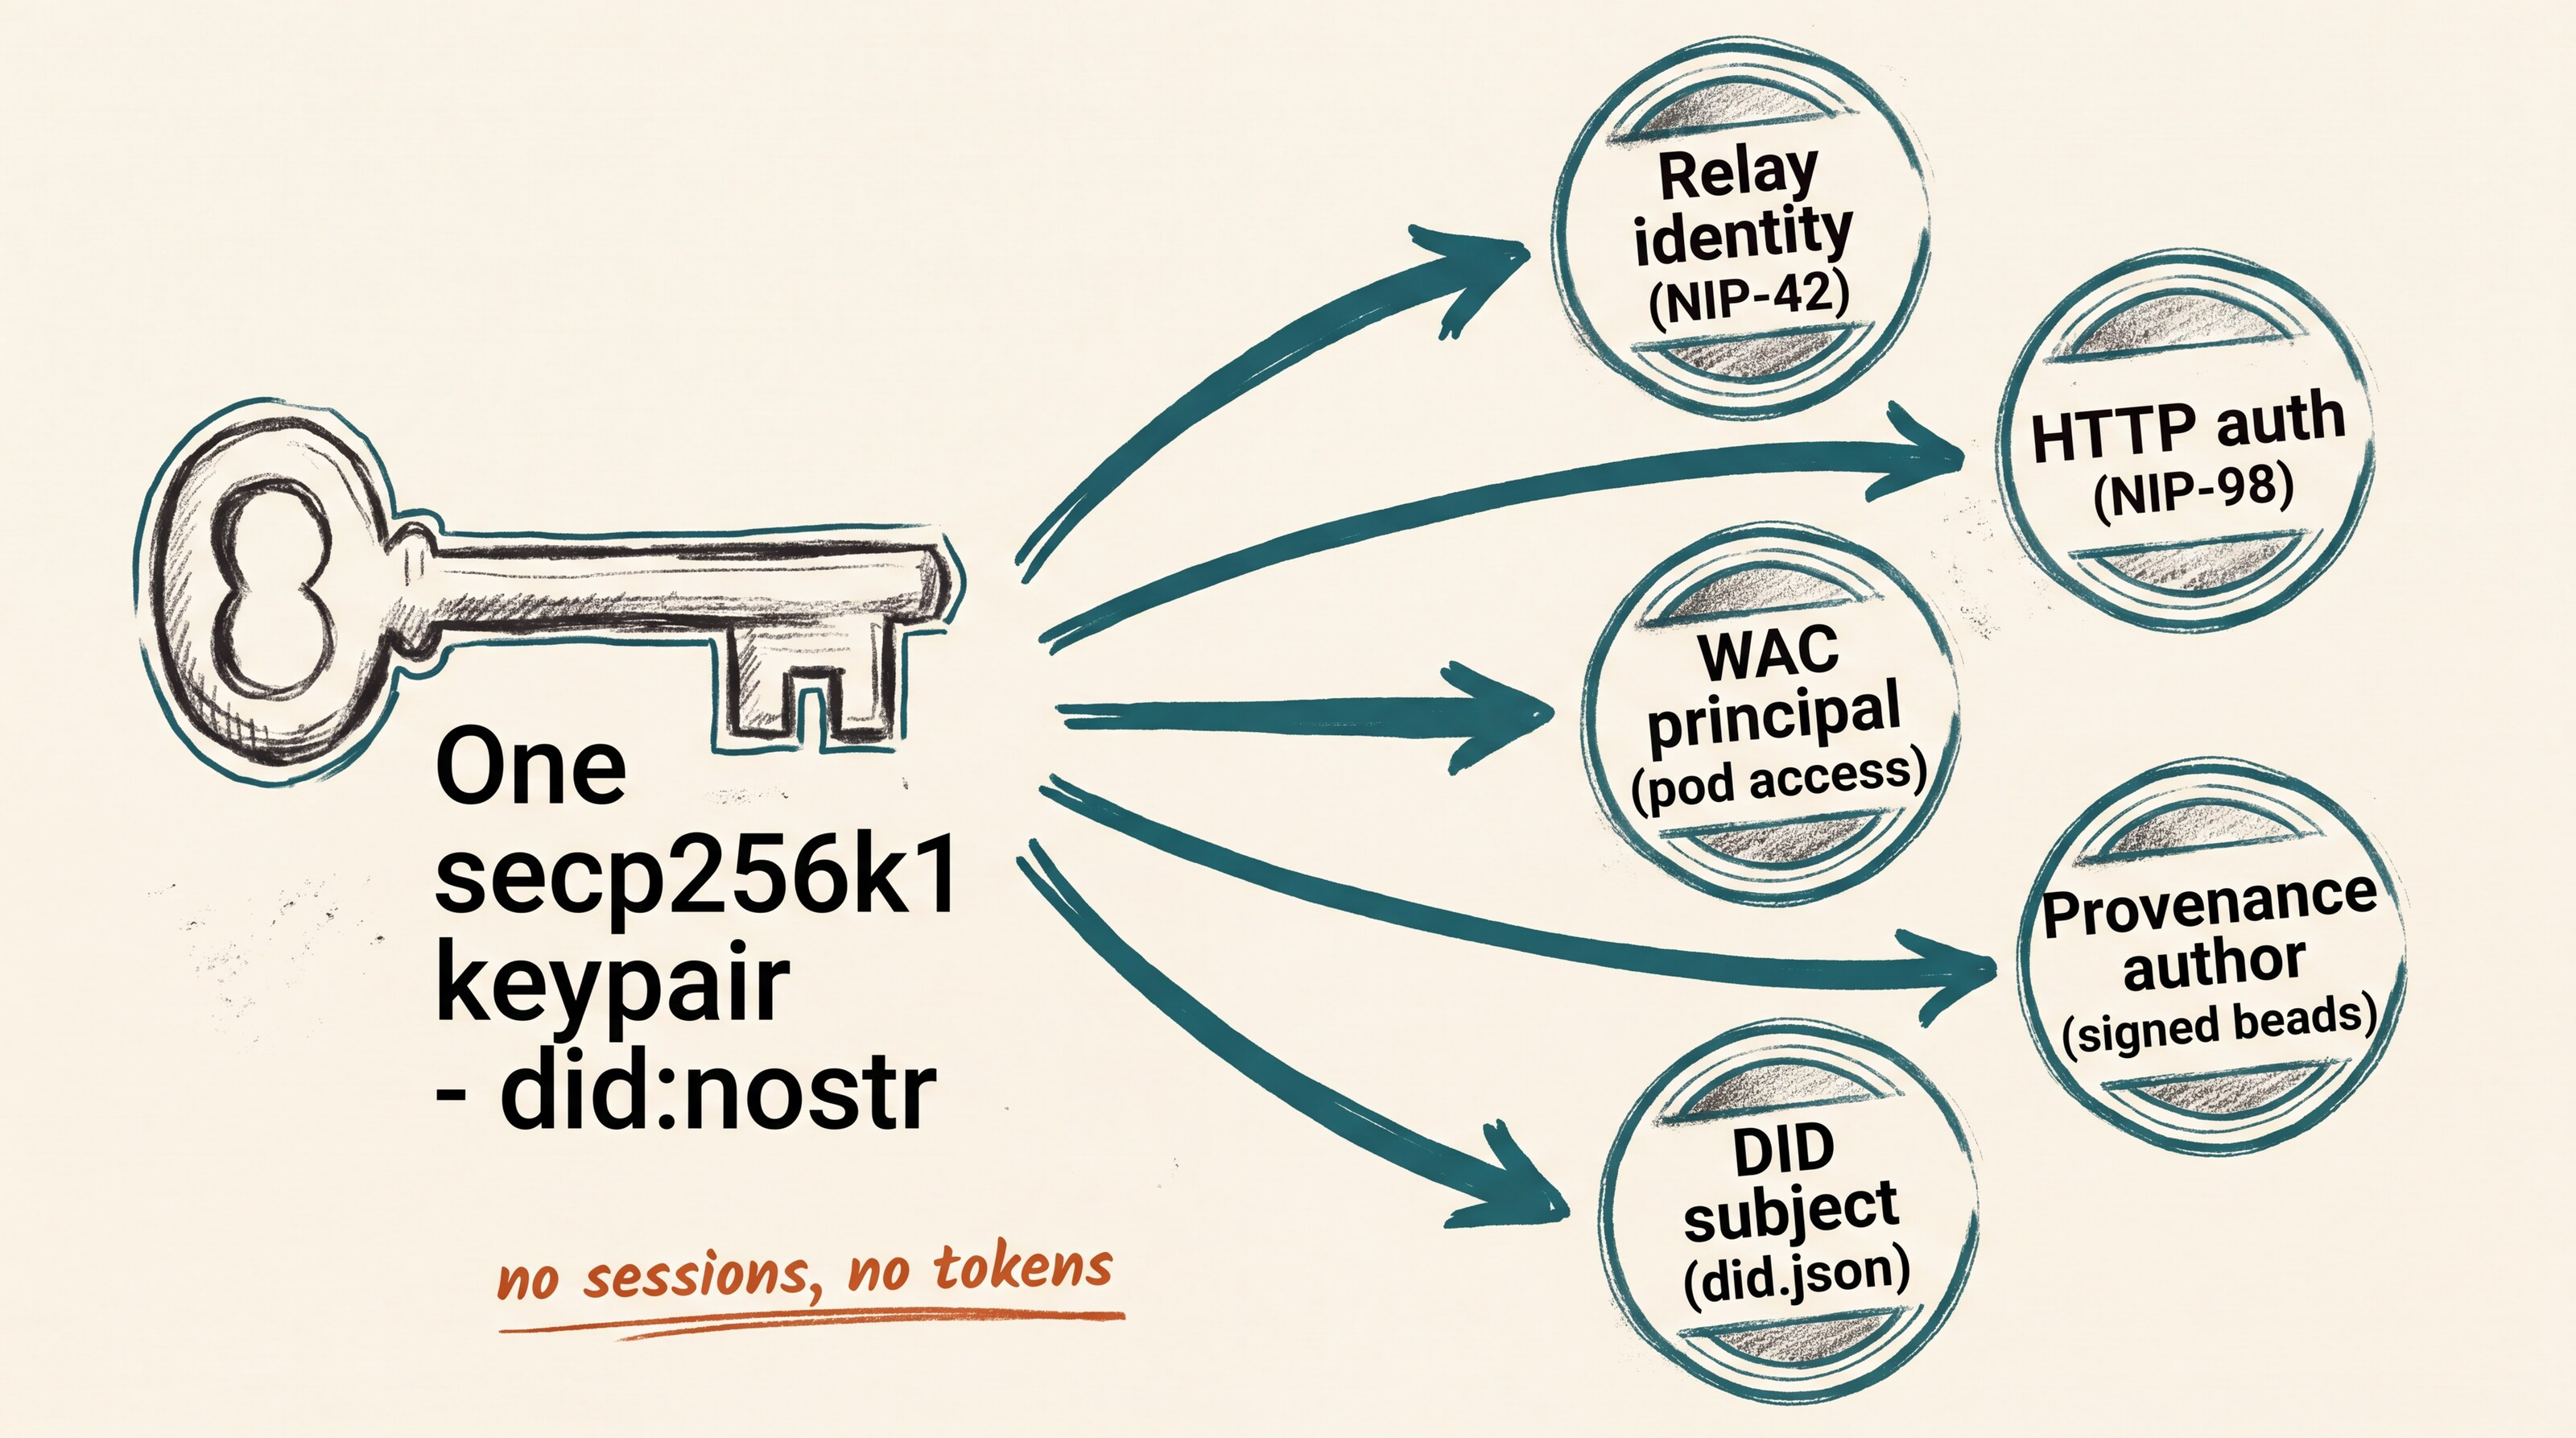
\includegraphics[width=0.88\textwidth]{nb-identity-spine.jpg}
\caption{The identity collapse, drawn: one secp256k1 keypair serving as relay identity, HTTP-auth identity, WAC principal, provenance author, and DID subject: no sessions, no tokens. Illustration in the house sketch style.}
\label{fig:identity-spine}
\end{figure}

\begin{definitionbox}[title={The identity collapse}]
Conventional systems carry a different identity at each trust boundary: a session cookie for the web tier, an OAuth token for the API, a service account for storage, a signing key for audit. Each boundary needs a translation step, and each translation step is a place where identity can be lost, forged, or confused. The \texttt{did:nostr} spine collapses all of these into one secp256k1 keypair. The relay identity, the HTTP-auth identity, the WAC principal, the provenance author, and the DID subject are the same 64 hex characters. Provenance, access control, and message routing then share one answer to the question ``who did this?''
\end{definitionbox}

The canon asserts NIP-42 relay authentication more strongly than the code currently enforces it. The 2026-07-03 reconciliation found that the forum relay advertises \texttt{auth\_required:false} and gates by a pubkey allowlist rather than completing a NIP-42 AUTH challenge-response round-trip. The relay-identity surface, in other words, is asserted at the level of the design and approximated at the level of the deployed worker. Chapter~\ref{ch:forum-governance} carries the detail; the point here is that the identity spine is a strong contract with one currently soft enforcement point.

\section{Judgment Broker as a Distributed Capability}

Chapter~\ref{ch:role-transformation} coined the \meshterm{judgment broker} role and Chapter~\ref{ch:governance} described the embedded governance that gives it teeth. The canon turns both into structure. \texttt{ADR-003} and the judgment-broker PRD state the design in one sentence: the broker is a capability that emerges from the coordination of four substrates, not a service that any one of them runs. nostr-rust-forum owns the domain model, the human decision surface, and the relay gating rules; AgentBox owns the agent runtime, the relay consumer, and decision application; VisionClaw owns enrichment gating over the knowledge graph; and the Nostr relay mesh is the transport. The event kinds \texttt{31400}--\texttt{31405} are the wire protocol that binds them. Agents write \texttt{31400} (PanelDefinition) and \texttt{31402} (ActionRequest); humans write \texttt{31403} (ActionResponse); the relay enforces the separation, so an agent key cannot sign a decision and a human key is required for one.

The decision itself carries one of six outcomes in the domain model (approve, reject, amend, delegate, promote, and precedent), though the canon is honest that only approve and reject are handled at runtime today, with the remaining four logging a warning and deferring their workflows to a follow-up specification. The promote and precedent outcomes in particular imply a precedent-replay system, letting an agent query past decisions rather than re-ask, that does not yet exist.

\begin{keyinsight}[title={Why no single repository owns the broker}]
\texttt{ADR-003} records three rejected alternatives, each rejected for a structural reason. A \emph{single-service broker} was rejected because it recreates the centralised bottleneck the federation exists to avoid; every decision would route through one service regardless of domain. A \emph{broker inside VisionClaw only} was rejected because the human decision surface, panel rendering, and response signing belong to the forum, and VisionClaw has no user-facing decision UI. A \emph{broker inside AgentBox only} was rejected because enrichment review needs knowledge-graph context that only VisionClaw holds, and duplicating the graph into AgentBox would break the single-source-of-truth principle. The broker is distributed because its responsibilities genuinely live in different places, and forcing them into one repository would fight the architecture rather than serve it.
\end{keyinsight}

The completion story is more honest in the third edition than in the first. Earlier documents described the broker as ``65 per cent implemented,'' and the 2026-07-03 closeout found that framing understates current state: two of the three named gaps are closed. Decision application (\texttt{handleGovernanceDecision}) is implemented and mints PROV-O provenance; five governance MCP tools ship in AgentBox.

The distributed \texttt{BrokerActor} is not an open gap but a superseded design, and \texttt{ADR-130} says so in as many words. It exists only on the unmerged \texttt{crashbug} freeze-debugging branch, bound to a Neo4j store this stack does not run, while main deliberately took \texttt{ADR-110} ACSP in its place: a stateless case producer, an inline decide-and-inbox handler, and an \texttt{ElevationActor} with a real fenced Oxigraph write-back. The storage-agnostic domain kernel beneath that dead actor --- the \texttt{BrokerCase} aggregate and its \texttt{DecisionOrchestrator} --- was cherry-picked onto main's ACSP case queue; the actor transport was left behind on purpose. The last mechanical seam, joining the pending-case producer to the REST decision projection so \texttt{GET /api/broker/inbox} shows open work and each decision projects to the forum as a \texttt{kind-31403} event, landed on 10 July 2026 (\texttt{ca145a1ce}). Chapter~\ref{ch:role-transformation} carries the front-end story, where the larger gap remains: the broker still has no decision canvas inside VisionClaw's own client.

\section{Provenance by Construction}

The canon's provenance claim is structural: every write is signed, every event is content-addressed, and every governance decision is an immutable Nostr event carrying a \texttt{prior\_decision\_id} chain that an auditor can traverse back to first principles. Provenance beads (kind \texttt{30001}) are content-addressed records; PROV-O activity records link a decision event to the agent action it authorised; git-marks record each pod write as a commit; and block-trails optionally anchor high-value records to Bitcoin via a taproot commitment (BIP-341), giving an externally verifiable receipt that even an adversarial party can check.

Provenance is a property present at the moment of writing, not a log appended afterwards. The graph is the audit trail.

Decisions inherit the same append-only discipline as the ledger beneath them. The judgment-broker domain model states it as an invariant: a \texttt{DecisionOutcome} is immutable once published, the Nostr event is the audit trail, and there is no undo --- only new events that supersede. Correction happens forward. A mistaken approval is not deleted or edited; a later signed event references it and overrides it, and both remain visible in the chain. This is the same guarantee git and the block-trail provide, applied to the governance layer: history accumulates, it does not rewrite.

That guarantee has one unspecified edge, and the canon is candid about it. The model says a Decision may be superseded but never says who holds the authority to publish the superseding event, or under what conditions. The mechanism for correction exists; the policy governing who may invoke it does not.

Provenance and value are designed to travel the same rails. Once every actor is a \texttt{did:nostr} identity and every write is anchored, the canon argues, the mesh can move value and trust between sovereign parties without an EVM, a bridge, or a custodian. The single keypair that authors provenance is also the WAC principal, the relay identity, and a payment account: a \texttt{did:nostr}-keyed HTTP~402 web-ledger meters value per request, Lightning and L402 rails carry the micropayments, and a taproot anchor makes a spend receipt as durable as the Bitcoin chain it settles on. This is the ecosystem's longest-horizon claim, and it is the least proven; the point for this chapter is only that identity, provenance, and settlement are designed to be one keyed rail rather than three, so that the audit trail and the money trail cannot diverge.

\section{Where Judgment Happens, and Where It Only Shows}

The canon draws a sharp line between the surface where a human rules and the surfaces where a human watches. Judgment happens in exactly one place: the forum. nostr-rust-forum owns the domain model, renders the panel, and signs the \texttt{31403} Decision, and only a human key may produce that event. Every scenario the canon walks through (climate consortium, drug discovery, creative production) routes the human decision through the same forum chokepoint.

That single locus is deliberate: it keeps the one authority-bearing action in one auditable place rather than scattering approval across every client.

The other surfaces are for observation and command, not decision. VisionClaw's desktop and XR clients render agent actions as beams and make blocked or approved states visually obvious through semantic physics, but no canon text gives them decision authority; a human watching the graph sees the consequences of decisions made in the forum. Voice occupies a third position that the canon added deliberately in 2026: a push-to-talk command captures the currently selected agent node and dispatches a \emph{scoped} ActionRequest to that agent's \texttt{did:nostr}, which is a least-authority choice: voice is agent-command ingress and never a channel for the human Decision itself.

Two honesty notes belong here. The voice-to-actor binding is documented more firmly than the code shows, and it depends on a contract that is currently broken, because live agent-actor nodes are keyed by \texttt{task\_id} rather than by \texttt{did:nostr} and so cannot yet be addressed by an ActionRequest. And the canon is silent on whether a decision observed in XR carries any different assurance than one rendered in the 2D forum, given that both ride the same relay transport. Chapters~\ref{ch:technical-substrate} and~\ref{ch:forum-governance} carry the surface-by-surface detail.

\section{Governance as an Accelerant}

The canon's wager, stated in the README and inherited directly from Chapter~\ref{ch:governance}, is that clean escalation makes the mesh faster. When an agent knows its authority boundary and surfaces exceptions cleanly, the roughly 90 per cent of decisions that need no human judgment flow without friction, and the roughly 10 per cent that cross a boundary arrive as a signed ActionRequest carrying context, evidence, and provenance. The human is asked a well-formed question at exactly the moment their judgment is load-bearing, rather than being asked to rubber-stamp everything or trust everything.

The wager has empirical support the report develops elsewhere. \textcite{Pereira2026Playbook}, surveying successful enterprise deployments, found that an escalation operating model, where agents act by default and surface exceptions, produced roughly 71 per cent median gains against roughly 30 per cent for an approval-on-every-output model. The canon's authority-boundary contract is the mechanism that makes escalation the default rather than the exception, and Chapter~\ref{ch:ecosystem-roadmap} commits to measuring whether it delivers that gain in DreamLab's own deployment.

This is the point of the whole part. The judgment broker of Chapter~\ref{ch:role-transformation} and the embedded governance of Chapter~\ref{ch:governance} are, in the canon, not slideware. They are an authority-boundary contract and a six-kind wire protocol with relay-enforced signing rules. The canon is those two chapters made structural --- the human side of what \textcite{Liu2026} calls an interface organisation (Chapter~\ref{ch:coordination-economics}), written down as code contracts rather than as policy. The measure of whether the wager pays off is empirical, and Chapter~\ref{ch:ecosystem-roadmap} states the falsification conditions in advance.

\section{How the Canon Keeps Itself Honest}

A contract layer is only worth the enforcement behind it. \texttt{ADR-002} gives the canon three instruments for keeping its own claims from inflating. The compatibility matrix is the human-readable source of truth for cross-repository identity, mesh, pod, governance, and verification posture, kept short enough to review in one sitting. Coordinated releases must publish a machine-readable manifest under \texttt{docs/releases/}, so a release claim becomes auditable against specific repository SHAs rather than a paragraph of prose.

And the mesh smoke test is the promotion gate: a capability moves from \texttt{integrated} to \texttt{federation-verified} only when the end-to-end path runs, not when the design document reads complete. Shared fixtures are checked byte-for-byte against SHA-256 checksums during release qualification, so a protocol contract cannot drift between substrates without the drift being caught mechanically.

The instruments work because they are used adversarially against the canon's own optimism. Two reconciliation passes bracket this edition. The 2026-05-29 pass closed several long-standing gaps with runtime evidence: the beam actor wired at boot, the \texttt{31402} dispatcher shipped, forum-originated decisions applied with PROV-O provenance. The 2026-07-03 pass then found the register stale in both directions: it confirmed those closures and it sharpened the evidence on what remains open, correcting an over-optimistic federation tally downward in the same document that recorded genuine progress. A canon that only ever revised its claims upward would be a marketing instrument. This one revises in whichever direction the code points, which is what makes its remaining claims worth trusting.

\section{What the Canon Asserts and the Code Does Not Yet Enforce}

The canon has become notably more self-critical across its reconciliations. The 2026-07-03 closeout confirmed several prior gaps closed with sharper evidence, and confirmed that others remain open, also with sharper evidence. Two of the open ones are principles the canon asserts as design commitments while the code enforces something weaker, and both belong to the sovereignty story the ecosystem sells.

\begin{cautionbox}[title={Two principles the canon states but the code does not yet enforce}]
\begin{itemize}
  \item \textbf{The pod mandate is not revocable in code.} The canon specifies that an agent writes to a user's pod \emph{as itself}, under a scoped, revocable WAC \texttt{acl:agent} mandate (\texttt{urn:agentbox:mandate}), never by holding the user's private key. The least-authority design is real and important. What is missing is the revocation: in solid-pod-rs's WAC evaluator the mandate is a static, non-expiring ACL grant with no expiry field and no revocation path. The revocability is espoused in prose and unwired in the evaluator.
  \item \textbf{No authority is defined for superseding a Decision.} Decisions are immutable-but-supersedable, yet the canon never names who may publish a superseding event, nor under what conditions. There is no specified appeal or revocation mechanism once a Decision is signed, and no rule for resolving two humans who respond to the same request.
\end{itemize}
\end{cautionbox}

These are named here, at the point where the principles are introduced, so that a reader is not left believing the canon and the code say the same thing. Related overstatements appear in place above: the NIP-42 relay gate is currently a pubkey allowlist, and this edition's July snapshot caught the flagship elevation loop opening its human-approval case without the Whelk consistency gate and emitting no \texttt{ConceptElevated} closing event. Both were wired shortly after, on 10--11 July 2026: the approve arm now clears \texttt{WhelkInferenceEngine::check\_axiom\_set} fail-closed before a case opens, and a merged pull request now fires a terminal \texttt{concept\_elevated} event rather than the elevation being claimed at PR-creation (VisionClaw \texttt{43a12e401}), with the live merge-poll observation still owed. The systematic four-surface accounting of every such gap lives in Chapter~\ref{ch:gap-register}; the component chapters name their headline gaps and point there rather than reproduce it.

One silence is worth naming because it bounds the whole design. Every documented escalation path in the canon terminates at a human. There is no canon-level position on agent-to-agent judgment, on whether one agent's action can require another agent's sign-off rather than a person's. The judgment broker is, by construction, a human-in-the-loop mechanism, and the ecosystem has not yet asked what a mesh does when the volume of boundary-crossing actions outruns the humans available to judge them. That is a question for a later edition, and Chapter~\ref{ch:open-questions} is where the report keeps its unanswered ones.

The pattern across all of these is the one this report has argued for throughout. The canon states a strong principle, the code implements a weaker approximation, and the canon says so in its own reconciliation files rather than waiting to be caught. That is the discipline a contract layer is for. The honest version of what the ecosystem does is more defensible than the aspirational one, and it is the version the rest of this part reports.

\chapter{Forum: Where Judgment Lives}
\label{ch:forum-governance}

\epigraph{An approval that leaves no signature is a rumour. Judgment lives where the decision is signed, timestamped, and cannot be quietly rewritten.}{}

\section{Why Judgment Belongs in Async Text}

Every earlier chapter that argued for keeping a human in the loop reached the same practical question and left it open: where does the loop physically close? The vigilance problem of Chapter~\ref{ch:vigilance} shows that a human asked to watch a fast, mostly-correct agent in real time will drift into rubber-stamping. The governance argument of Chapter~\ref{ch:governance} asks for approval to be an accelerant rather than a bottleneck. Neither is achievable at a live console watching actions stream past faster than a person can read them. The forum answers with a deliberately slower medium: asynchronous, signed text.

Async text earns the role on three properties. It is legible, because a decision is a written artefact a second person can read months later and understand without replaying a session. It is auditable, because every request and every response is a signed Nostr event appended to a relay, so the record of who decided what, on what evidence, is the primary object rather than a log emitted beside it. And it is rate-limited by construction: the throughput of readable prose bounds how fast decisions can be demanded of a human, which is exactly the property a real-time dashboard lacks and exactly the property the vigilance literature says oversight needs. This is where \textcite{Liu2026}'s interface organisation stops being an abstraction. Their specification is that agent outputs enter human workflows only with evidence attached and human judgment mandatory at defined points; the forum is a literal implementation of that specification over a public-key message bus.

The medium also makes the signed record the object of coordination rather than a by-product of it. A request for a decision, the decision itself, and every later supersession are events with the same shape and the same signature discipline, so the trail a regulator or a teammate would want to reconstruct already exists as data the moment the decision is made. That is the strong form of the claim. Its honest weakness sits at the other end of the same pipe. The panel a human signs against today carries a title, a description, and action buttons, but no reasoning trace, no confidence figure, and no provenance from the agent that raised it, and the decision history the relay writes to \texttt{broker\_decisions} has no read endpoint at all. The audit substrate is genuinely present; the human-facing view into it, at the moment it would most help a person decide well, is the part still to build.

The forum's claim to be \emph{where} judgment lives is not rhetorical. VisionClaw's immersive client, surveyed in Chapter~\ref{ch:technical-substrate}, produces real \texttt{kind-31402} broker cases from its own runtime and then renders no surface for them at all: a human must leave the 3D scene entirely and open the forum web page to decide. Among the ecosystem's surfaces the forum is not one option for closing the loop. Today it is the only one that draws the decision on a screen a human can act on.

\section{Identity Without a Password Database}

The forum's identity model removes the asset every credential breach targets. There is no password store and no email column, because a WebAuthn passkey \emph{is} the account. The passkey's PRF extension deterministically derives the member's root Nostr key on-device, and that key never reaches the server. Identity is a \texttt{did:nostr} Multikey DID (\texttt{did:nostr:<x-only-hex>} with a single \texttt{Multikey} verification method), the same canonical form the wider did-nostr and create-agent tooling speaks, so a member's identity is portable across every system that implements the method. Purpose-scoped subkeys derive from the root through \texttt{derive\_subkey}, an HMAC-SHA-256 primitive tested identically in native and WASM builds (\texttt{ADR-094}), giving rotatable device and capability keys recoverable from the root alone. Signup issues a fully client-side printable recovery sheet (\texttt{ADR-095}); the private key is minted in WASM and does not touch the network.

One design choice keeps the identity portable without making the cryptography fragile: authentication reads the raw signature, never the document. NIP-98 for HTTP and NIP-42 for the relay verify a Schnorr signature against the raw event pubkey, so re-encoding the DID document can never move the auth path. Agents sit on the same substrate. An agent is a \texttt{did:nostr} subject exactly as a human is, commonly an \texttt{ADR-094}-derived subkey of an operator key, and it is admitted to the governance kinds only after an admin writes it into a registry (below). This is the substrate that Chapter~\ref{ch:gap-register} confirms is genuinely ahead of 2026 industry practice: cryptographic agent identity with relay-enforced registry gating and self-sovereign key custody, in a landscape where most production agents act with no verifiable identity of any kind and no ratified standard for agent self-identification yet exists.

The lifecycle around the root key is built for loss and rotation rather than assuming neither happens. A member may tear off per-device subkeys so that a stolen device is revocable without rotating the root identity (\texttt{ADR-099}), and the relay resolves a device key to its owning principal at the AUTH gate, so revocation takes effect at the enforcement point rather than only in a UI. There are no hardcoded admin keys: the first registrant becomes admin, and an operator onboards further members through single-use \texttt{/connect} magic links that generate the invitee's key in WASM without ever exposing an admin seed (\texttt{ADR-098}). Each of these is a place where a conventional forum would reach for a password reset, an email loop, or a server-held secret, and where this kit reaches for a signature instead.

\section{Access Is Data, Not Code}

Who may see and post to what is described entirely in one operator file, not in the kit's source. A deployment copies \texttt{forum.example.toml} to \texttt{forum.toml}, fills in its zones and cohorts, and changes no code. The zone list is serialised to a single \texttt{ZONE\_CONFIG} JSON blob that fans out to both enforcement points: the relay reads it as an environment variable and gates deny-by-default; the client reads the same JSON from \texttt{window.\_\_ENV\_\_} and draws the banner tiles. Because both sides read one description, the picture a member sees never lies about what they can reach.

Visibility has three settings and the relay honours all of them (Table~\ref{tab:zone-visibility}). A \texttt{public} zone is readable without authentication; a \texttt{locked} zone, the default, shows a greyed tile whose kind-40 definition is served so the tile can draw while its content stays withheld; a \texttt{hidden} zone is not enumerable at all, so a non-member cannot learn it exists. Read and write cohorts are separate, which yields the common pattern of an openly readable landing zone that only an inner circle may post to. When the config is absent the relay denies non-public reads: the system fails closed, so a misconfiguration cannot silently open a private zone. Cohorts gate an agent's ordinary board content the same way they gate a human's; they are orthogonal to the governance privilege described next, which the relay scopes by registry and admin status regardless of zone.

\begin{table}[h]
\centering
\caption{Zone visibility settings and what a non-member perceives}
\label{tab:zone-visibility}
\begin{tabularx}{\textwidth}{L{3.2cm} L{3.4cm} X}
\toprule
\textbf{Visibility} & \textbf{Listed to non-members} & \textbf{Definition and content served} \\
\midrule
\texttt{public} & Yes & Content readable without authentication \\
\addlinespace
\texttt{locked} (default) & Yes, as a greyed tile & Definition served so the tile draws; content withheld \\
\addlinespace
\texttt{hidden} & No & Neither definition nor content; existence not enumerable \\
\bottomrule
\end{tabularx}
\end{table}

The member reads the access model as furniture rather than as policy text. On arrival the client draws a wall of zone tiles generated from the same \texttt{ZONE\_CONFIG} the relay enforces from: enterable tiles for zones the viewer's cohorts open, greyed locked tiles for those they do not, and nothing at all for hidden zones. Inside a cohort-gated section the relay streams the group chat only after a NIP-42 AUTH handshake proves the cohort, and every identity in the room flows through one reactive resolver (display name, then profile name, then NIP-05, then a short pubkey), so a freshly seeded member with no metadata shows as a truncated key and fills in live the moment their kind-0 profile arrives. No raw hex lingers in the interface, and that single resolver path is the seam where an agent-disclosure badge belongs, once the canon requires agents to be visibly distinct from the humans they sit beside.

\begin{figure}[h]
\centering
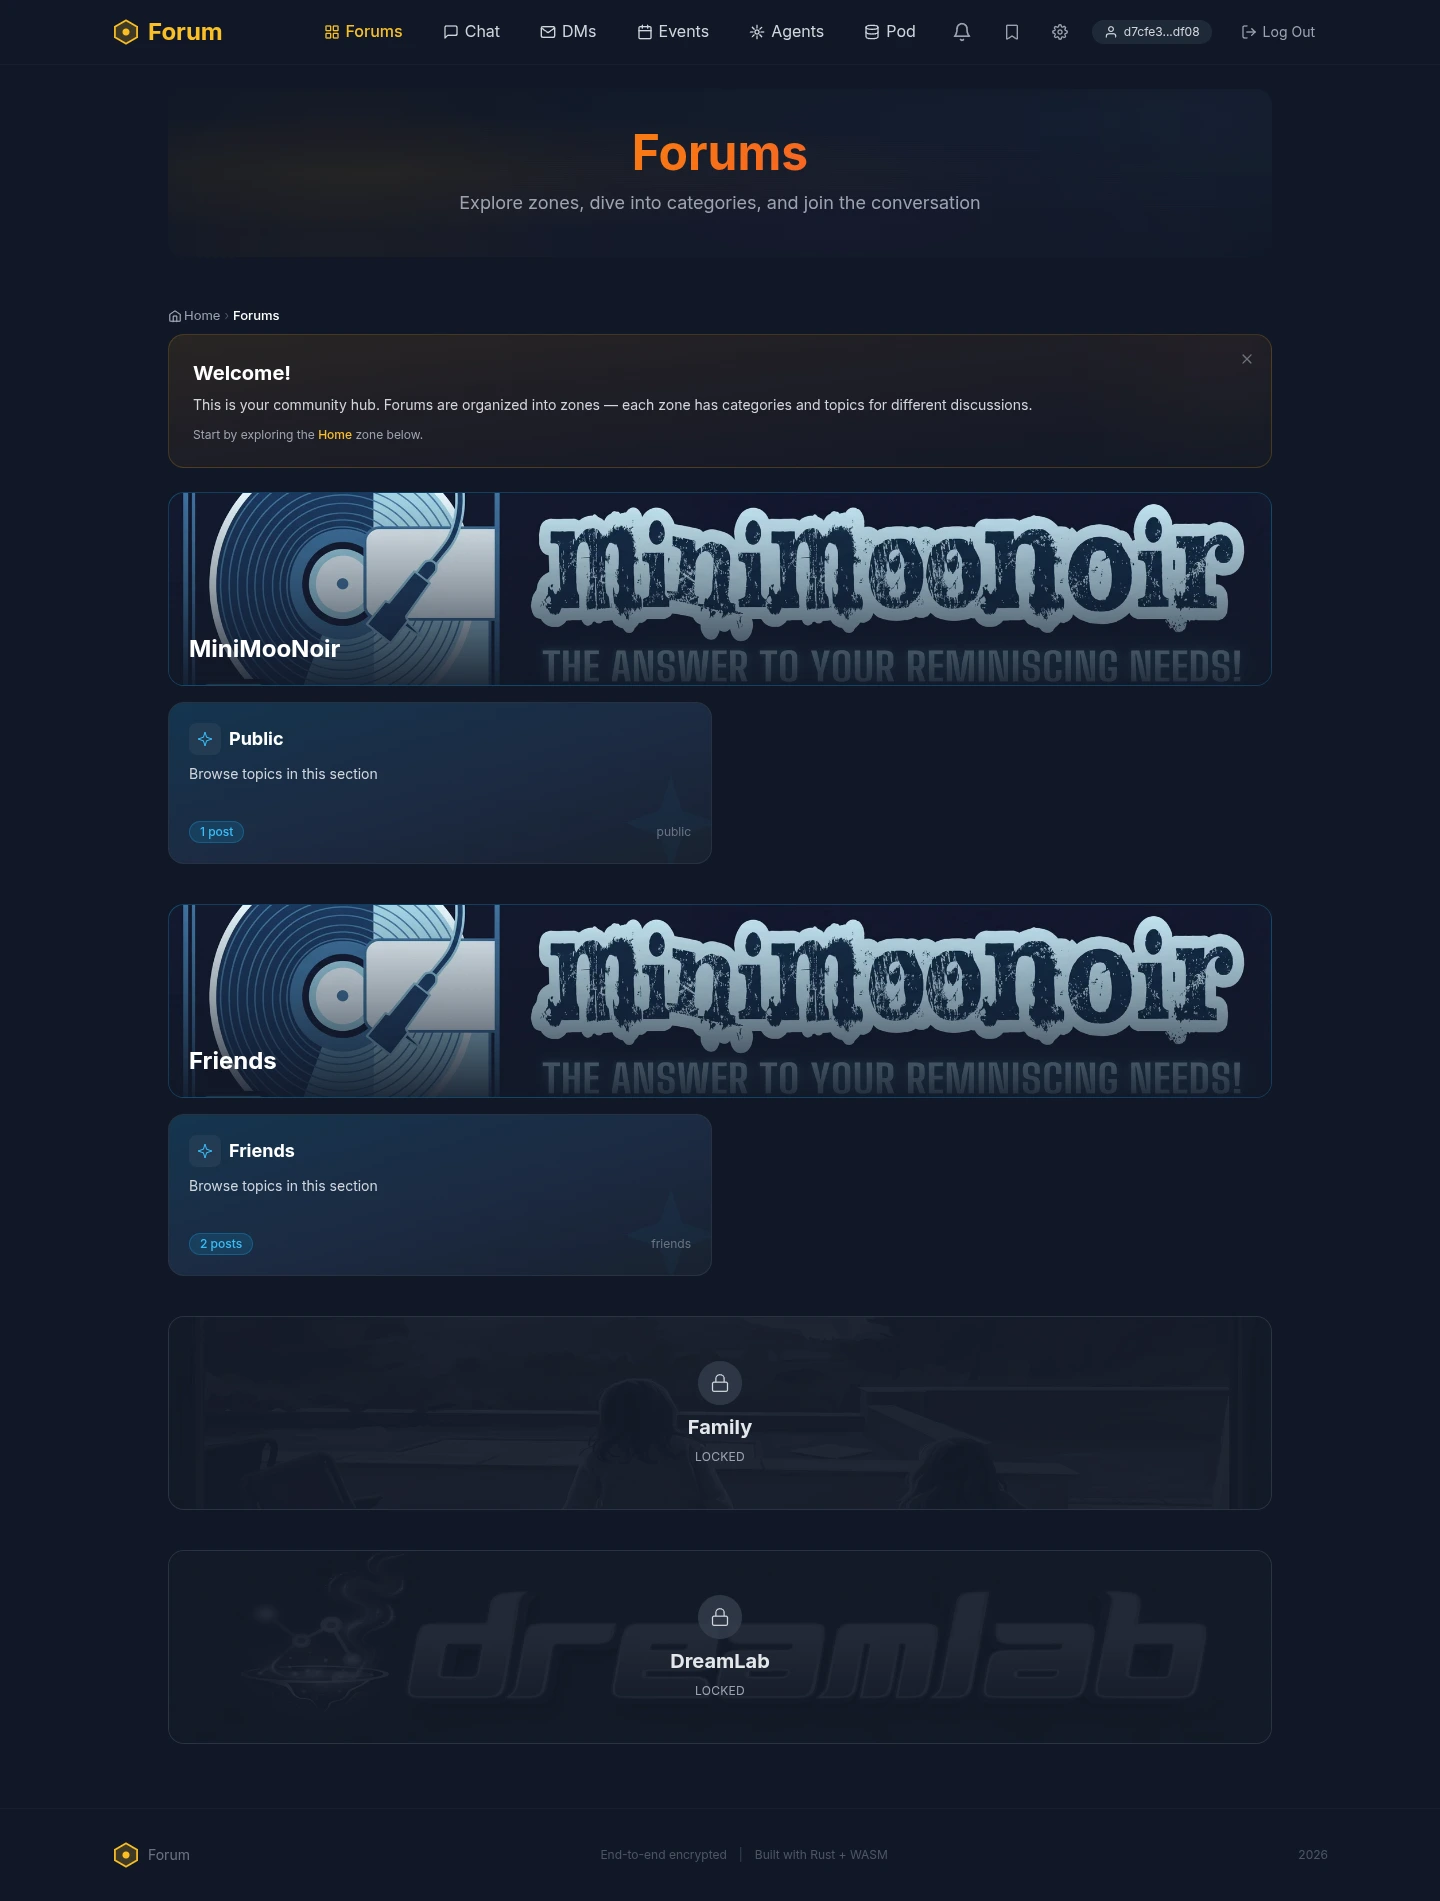
\includegraphics[width=0.72\textwidth]{shot-forum-zones.png}
\caption{The zone wall as a member sees it: enterable, greyed, and absent tiles drawn from the same \texttt{ZONE\_CONFIG} the relay enforces. Production screenshot.}
\label{fig:forum-zones}
\end{figure}

\section{Agent Control Surface Protocol}

The load-bearing mechanism is a six-kind protocol that turns any agent's request for a human decision into a signed, rendered card and turns the human's answer into a signed, appended event. It is wired end-to-end in shipping code, not relay-side scaffolding: an agent publishes a \texttt{PanelDefinition} and an \texttt{ActionRequest}, a reactive store in the Leptos client ingests the governance subscription, a human clicks Approve or Reject, and the client signs and publishes a \texttt{kind-31403} \texttt{ActionResponse} under the member's own \texttt{did:nostr} key. The response is a real cryptographic decision, not a UI toggle.

\begin{definitionbox}[title={The Agent Control Surface Protocol (ACSP)}]
Six parameterised-replaceable event kinds carry the human-in-the-loop loop. Kinds 31400 (\texttt{PanelDefinition}), 31401 (\texttt{PanelState}), 31402 (\texttt{ActionRequest}), 31404 (\texttt{PanelUpdate}) and 31405 (\texttt{PanelRetired}) are published by an agent and admitted only from a pubkey holding an active \texttt{agent\_registry} row. Kind 31403 (\texttt{ActionResponse}) is the human's signed decision. The kinds are declared once in \texttt{nostr-bbs-core} and enforced at relay ingress; the NIP-11 document advertises them under a \texttt{nostr\_bbs.agent\_control\_surface} block so an agent can discover the surface and its registry gate.
\end{definitionbox}

Table~\ref{tab:acsp-kinds} states the admission rule for each kind. The role separation is the point: agent keys carry the requests, and no agent key can sign an approval, because the relay hard-gates \texttt{kind-31403} to admins through a \texttt{governance\_response\_blocked} check that fires independently of what either client's UI permits the user to attempt.

\begin{figure}[h]
\centering
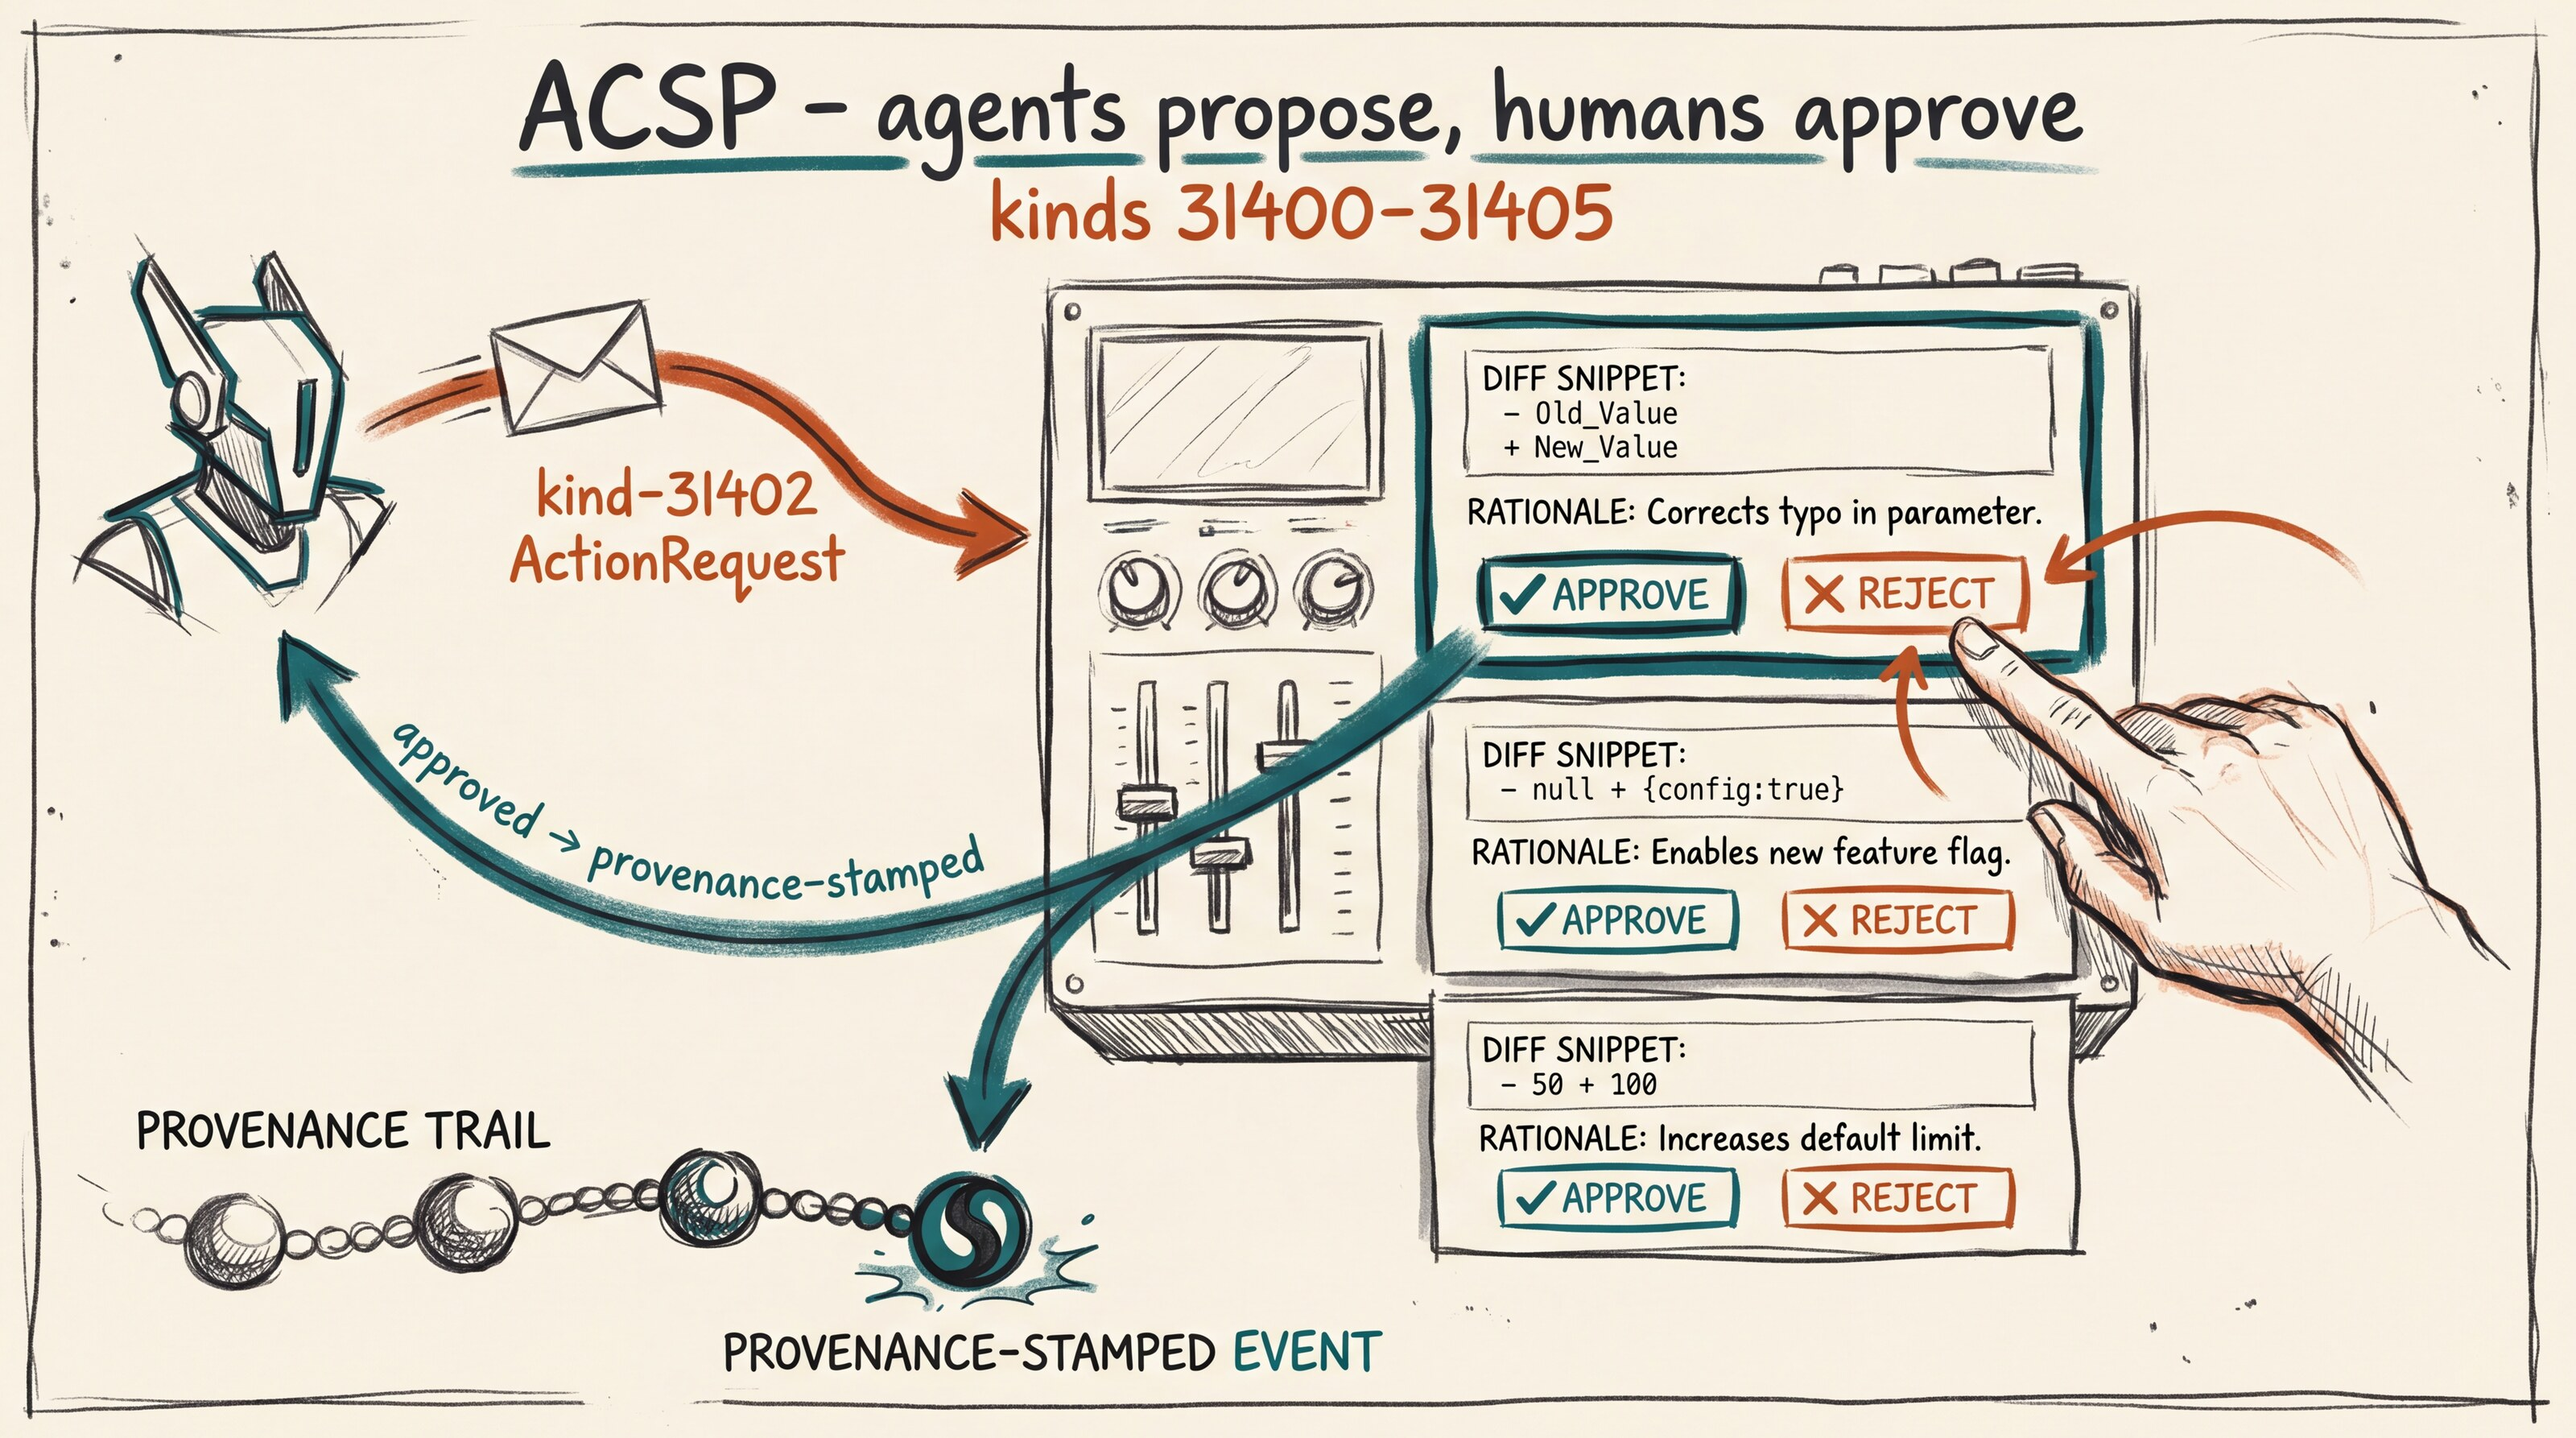
\includegraphics[width=0.92\textwidth]{nb-acsp-workbench.jpg}
\caption{The judgment loop: an agent's signed \texttt{kind-31402} ActionRequest arrives as a rendered card; the human's Approve or Reject returns as a signed \texttt{kind-31403} decision and lands on the provenance trail. Illustration in the house sketch style.}
\label{fig:acsp-workbench}
\end{figure}

\begin{table}[h]
\centering
\caption{ACSP event kinds and their relay admission rules}
\label{tab:acsp-kinds}
\begin{tabularx}{\textwidth}{L{1.8cm} L{3.0cm} X}
\toprule
\textbf{Kind} & \textbf{Name} & \textbf{Publisher and relay admission rule} \\
\midrule
31400 & PanelDefinition & Registered agent; rejected at ingress without an active \texttt{agent\_registry} row \\
\addlinespace
31401 & PanelState & Registered agent \\
\addlinespace
31402 & ActionRequest & Registered agent; projected to \texttt{broker\_cases} on admission \\
\addlinespace
31403 & ActionResponse & Human, admin only; \texttt{governance\_response\_blocked} rejects any non-admin key, agent or member \\
\addlinespace
31404 & PanelUpdate & Registered agent \\
\addlinespace
31405 & PanelRetired & Registered agent \\
\bottomrule
\end{tabularx}
\end{table}

Awareness is push-based and the persistence is deliberately plain. A live subscription over the relay WebSocket feeds the client's reactive \texttt{PanelRegistry}, so a new panel or action appears without a refresh. On admission the relay projects each \texttt{ActionRequest} into a \texttt{broker\_cases} row and each accepted \texttt{ActionResponse} into an append-only \texttt{broker\_decisions} row, with \texttt{broker\_roles} recording who may broker. The tables co-reside in one D1, which is what makes the whole loop of request, projection, decision and state update a set of ordinary rows a query can walk rather than a bespoke workflow engine. The auth worker exposes read APIs for cases and roles. The gap the survey flags, which the repository's own flow diagrams also flag as Finding~5, is that \texttt{broker\_decisions} has no read endpoint, so the one table that is the audit trail is the one table with no supported way to read it back.

Bringing an agent identity online was once a four-call seed script with a partial-failure window between allowlisting a pubkey and registering it. \texttt{ADR-097} collapses the two admin-side writes into one operation: \texttt{POST /api/governance/agents/provision} upserts the \texttt{whitelist} and \texttt{agent\_registry} rows in a single D1 \texttt{batch()}, all-or-nothing and idempotent on the pubkey, so a re-provision is a safe way to update an agent's cohorts. The endpoint never receives the agent's private key; key material and the agent's own signed kind-0 profile stay client-side, keeping the self-sovereign identity boundary clean while the server owns only membership and registry state. Whether an agent may act at all is therefore an admin-only \texttt{curl} or config-file act with no calling UI in the kit, which places the governance-of-governance step of deciding who governs outside the very surface the human-facing documentation presents as the operator's console.

\begin{keyinsight}[title={The relay is the sole enforcement point}]
Neither client's UI is trusted. A non-admin who reaches an Approve button in the retro client still has their \texttt{kind-31403} rejected server-side with an inline reason (\texttt{blocked: admin-only governance action response}); an unregistered agent's panel is dropped at ingress. Every governance guarantee, meaning who may request and who may decide, is a property of \texttt{nip\_handlers.rs} on the relay Durable Object, not of anything the browser renders. This defence-in-depth posture, never trusting the client, is what lets the decisions form an immutable signed audit trail rather than a record of what a UI happened to allow.
\end{keyinsight}

Two honest limits sit under the polished parts, and the code-verified survey is blunter than the architecture document. First, the richer case lifecycle the documentation advertises is not reachable. \texttt{nostr-bbs-core} defines a fully unit-tested \texttt{DecisionOrchestrator} with delegate, promote and precedent transitions, but nothing outside its own test module calls it; the live relay projection understands only \texttt{approve} to resolved and \texttt{reject} to rejected, and any other action a panel might expose parks the case in \texttt{under\_review} indefinitely. The \texttt{architecture.md} state diagram depicts transitions that no end-to-end path can trigger. Second, and more consequential for the ecosystem's framing, the shipping forum client gates the entire \texttt{/governance} route to admins: \texttt{AdminGatedGovernance} bounces any authenticated non-admin to the forums with a toast before the page mounts, which contradicts the same document's Trust and Gating table granting ordinary members a panel view. The kit advertises a universal human-in-the-loop plane; what ships is an \meshterm{operator-in-the-loop} plane, where the flagship chokepoint reads ``forum, then an admin decides'' in place of ``forum, then a human decides''. Chapter~\ref{ch:gap-register} carries this as a headline gap alongside the absence of any visible agent badge, the one point on which the disclosure literature is unanimous.

A subtler provenance defect compounds the first. The forum client publishes the signed \texttt{kind-31403} fire-and-forget and flips the card to ``Response sent'' the instant local signing succeeds, without waiting for the relay's NIP-01 OK frame. Because the relay independently rejects invalid responses, an operator can believe they governed an action when nothing was accepted. The retro BBS client already does this correctly through \texttt{publish\_with\_ack}, surfacing the rejection reason inline; on a governance surface, confirming a decision the relay refused is a trust-calibration failure, not a cosmetic one.

\section{Calendars Projected Per Viewer}

The tiered NIP-52 calendar shows that the same config-as-access model extends to time. Calendar events bind to a zone and optionally to a shared venue, and the relay's projector decides, for every viewer-and-event pair, one of three outcomes: the full signed event, an anonymised free/busy block, or omission so complete the viewer never learns the event exists. A member of a neighbouring cohort holding an event at a shared venue is projected down to \texttt{to\_free\_busy()} output of start, end, venue and a busy flag, with title, location, participants, content and even the signature stripped server-side, so the result is a derived view rather than the signed original. Off-site private events are simply omitted. The trust boundary is that neighbours can see the room is booked without seeing whose party it is.

Table~\ref{tab:calendar-projection} is the operator-approved projection matrix, pinned in place by twenty-five unit tests. Two details make the boundary hold under adversarial input rather than only in the common case. RSVPs are served only when the viewer's tier for the target event is Full, so a participant list cannot leak through a free/busy block; and the target event's zone and venue resolve exclusively from the stored referenced event, so a spoofed zone tag mirrored onto an RSVP cannot widen access. The projection is the complete access decision for calendar kinds and is deny-by-default for unknown zones, which is the enforcement discipline the security-front-loading finding of Chapter~\ref{ch:ecosystem-roadmap} calls for.

\begin{table}[h]
\centering
\caption{Calendar projection outcome per viewer cohort and event zone}
\label{tab:calendar-projection}
\begin{tabularx}{\textwidth}{L{2.8cm} X X X X X}
\toprule
\textbf{Viewer} & \textbf{family} & \textbf{business} & \textbf{friends} & \textbf{public} & \textbf{unknown} \\
\midrule
admin / owner & full & full & full & full & full \\
\addlinespace
family & full & full & full & full & full \\
\addlinespace
friends & free/busy* & free/busy* & full & full & omit \\
\addlinespace
business & omit & full & omit & full & omit \\
\addlinespace
no cohort / anon & omit & omit & omit & full & omit \\
\bottomrule
\end{tabularx}
\end{table}

The asterisk marks the one conditional cell: friends see family and business events as free/busy only at a recognised shared venue, and off-site events are omitted, so a friend learns of venue blocking but never of private off-site time. Shared venues are operator-defined in \texttt{forum.toml}; the kit ships generic \texttt{primary} and \texttt{secondary} examples so nothing about a real deployment's places is baked into the source.

\section{Moderation and the Retro Write Path}

Moderation is relay-enforced rather than advisory: NIP-56 reports (kind-1984) are validated at ingress by the relay worker, and the inactivity-demotion sweep runs on a cron against the whitelist, so a report or a lapse changes what the relay will serve rather than merely annotating a UI. The forum also ships a second, deliberately minimal client (a phosphor-CRT retro BBS surface at \texttt{/community/bbs/}), and its write path is instructive precisely because it was documented honestly when it diverged from its own plan.

\texttt{ADR-105} draws a principle before it draws a feature: a BBS surface requires identity only when it reads private data or writes a signed event. Everything else, including the masthead, the help screen, read-only board and roster rendering, and the door games, must work for a logged-out viewer. Door games are the sharp case. The first of them, a faithful sentry-gun deck adapted from an MIT-licensed project, is a pure client-side overlay launched by a custom DOM event and touching no relay, no signer and no key, which is the seam by which further self-contained toys attach without dragging any of them through the identity path. The line the ADR draws is that public surfaces stay public and only signed writes demand a key.

The write path itself is the honest part. \texttt{ADR-105} originally decided the BBS would never hold key material and would delegate signing to the forum through a same-origin \texttt{sign()} seam. The shipped M2 write path instead holds a \texttt{Keypair} directly through the kit's NCC-audited \texttt{PrfSigner}, and the ADR's 2026-07-03 amendment records the change in place. Because the two clients are served same-origin, any script that could reach a \texttt{sign()} bridge can already read the session key, so a direct hold and a delegated seam sit on the identical trust boundary, and the in-memory path fails closed when no signer is present. The amendment also flags, rather than letting the divergence pass silently, the residual boundary it did not close: a passkey user who generates a fresh in-memory key signs under a distinct key, not the PRF-derived root. The retro client's governance action button signs and publishes its \texttt{kind-31403} through \texttt{publish\_with\_ack}, which is the relay-confirmed pattern the forum client still needs to adopt.

\section{One Use Case, Stated Plainly}

The README describes a universal human-in-the-loop control plane for any agent system. The distance between that phrase and current use should be stated without softening. Today the governance plane serves exactly one use case: ontology concept elevation, capped at five concurrent cases, decided on the forum web page by a single administrator role. Everything else the protocol makes possible, from multiple agent systems and multiple communities to graduated decisions richer than approve-or-reject and ordinary members participating in judgment, is either scaffolded, admin-gated, or unbuilt. The nine-endpoint governance REST API has no calling UI anywhere in the kit; provisioning and revoking the agents that may act is a \texttt{curl} or config-file operation, so the single most authority-laden step in the whole design sits outside the product surface the human-facing documentation advertises.

\begin{cautionbox}[title={What the governance plane does not yet do}]
\begin{itemize}
  \item Ordinary members can neither view nor decide governance panels in the forum client; the route is admin-only, so the ``distributed human judgment'' claim is presently a single-operator approval queue.
  \item Decisions are binary approve or reject; the delegate, promote and precedent lifecycle is unit-tested dead code, and a non-binary action parks a case in \texttt{under\_review} permanently.
  \item The forum client reports a decision as sent before the relay confirms it, so a rejected \texttt{kind-31403} can still read as success.
  \item A published decision is immutable by design, yet no supersede or appeal path is specified or built, so an operator who approves in error, or a member who would contest a call, has no defined recourse.
  \item Agents are visually indistinguishable from humans: no bot badge, and no display of the principal that authorised each agent.
  \item Governance events cannot cross relays. The \texttt{nostr-bbs-mesh} crate is scaffold-only, is not a dependency of the relay worker, and holds no agent-federation path, so each community's governance plane is an island (Chapter~\ref{ch:gap-register}).
\end{itemize}
\end{cautionbox}

The strengths and the gaps point the same way. The cryptographic substrate is real and ahead of the field: passkey-derived \texttt{did:nostr} identity, relay-enforced registry gating, atomic idempotent provisioning, and admin-only signed responses. The collaboration surface built on top of it is narrower than the canon claims, and in three places the survey verifies by direct read, narrower than the architecture document claims. The escalation-beats-approval evidence of \textcite{Pereira2026Playbook}, the vigilance evidence of \textcite{DellAcqua2023}, and the failure-taxonomy discipline of \textcite{Cemri2025} all argue for risk-tiered, evidence-carrying, confirmed decisions; the substrate to build them exists here, and the accounting of how much remains unbuilt is the subject of Chapter~\ref{ch:gap-register}.

\chapter{VisionClaw: the Embodiment Surface}
\label{ch:technical-substrate}

\epigraph{The honest version is more defensible and more credible.}{}

\section{A Working Knowledge Substrate}

VisionClaw is not a prototype, a whitepaper, or a concept rendering. It is the knowledge substrate of the DreamLab ecosystem: a Rust server with GPU-accelerated graph physics, an OWL~2 ontology engine with Whelk reasoning, and a multi-user WebXR client, in daily use by a creative technology team at DreamLab in Fairfield, Eskdale.

Within the ecosystem it plays a specific role. It is the embodiment and observation surface: the place where agent action is meant to become visible, so that a human can watch what the mesh is doing and see which parts need a human. Judgment happens elsewhere. The nostr-rust-forum (Chapter~\ref{ch:forum-governance}) owns the signed human decision. VisionClaw is where the operator looks; the forum is where the operator rules.

This chapter describes what the system is, what it does, and what it does not yet do. Every claim here is reconciled against the codebase as surveyed in July 2026, and where the shipping documentation and the code disagree, the code wins and the chapter says so at the point of the claim.

The embodiment surface has a longer ancestry than the codebase. It descends from a fifteen-year telepresence research programme run through the Octave mixed-reality laboratory at NICVE, and the constructs that programme measured --- co-presence, mutual gaze, proxemics, and the collaboration group size beyond which shared presence degrades --- are the same ones Chapter~\ref{ch:four-surfaces} uses to judge what this surface owes an operator. The question VisionClaw's desktop and headset put to a human, how to make distributed activity legible and shared inside one space, is the question that research pursued across two decades.

The ancestry has a precise first artefact. In 2017, Professor Rob Aspin ran an unpublished precursor in the Octave: a knowledge graph rendered and manipulated inside the laboratory's immersive space, nine years before the dual-graph demonstrations this chapter verifies (Figure~\ref{fig:chloe-octave}). The VisionClaw repository's own README credits that work directly. The through line from that room to this codebase is unusually literal --- the same idea, standing inside shared knowledge, carried from a physical multi-modal facility into a WebXR renderer, with the intervening years spent building the substrate the 2017 system had no access to: cryptographic identity, sovereign storage, and a mesh of agents to populate the graph.

\begin{figure}[h]
\centering
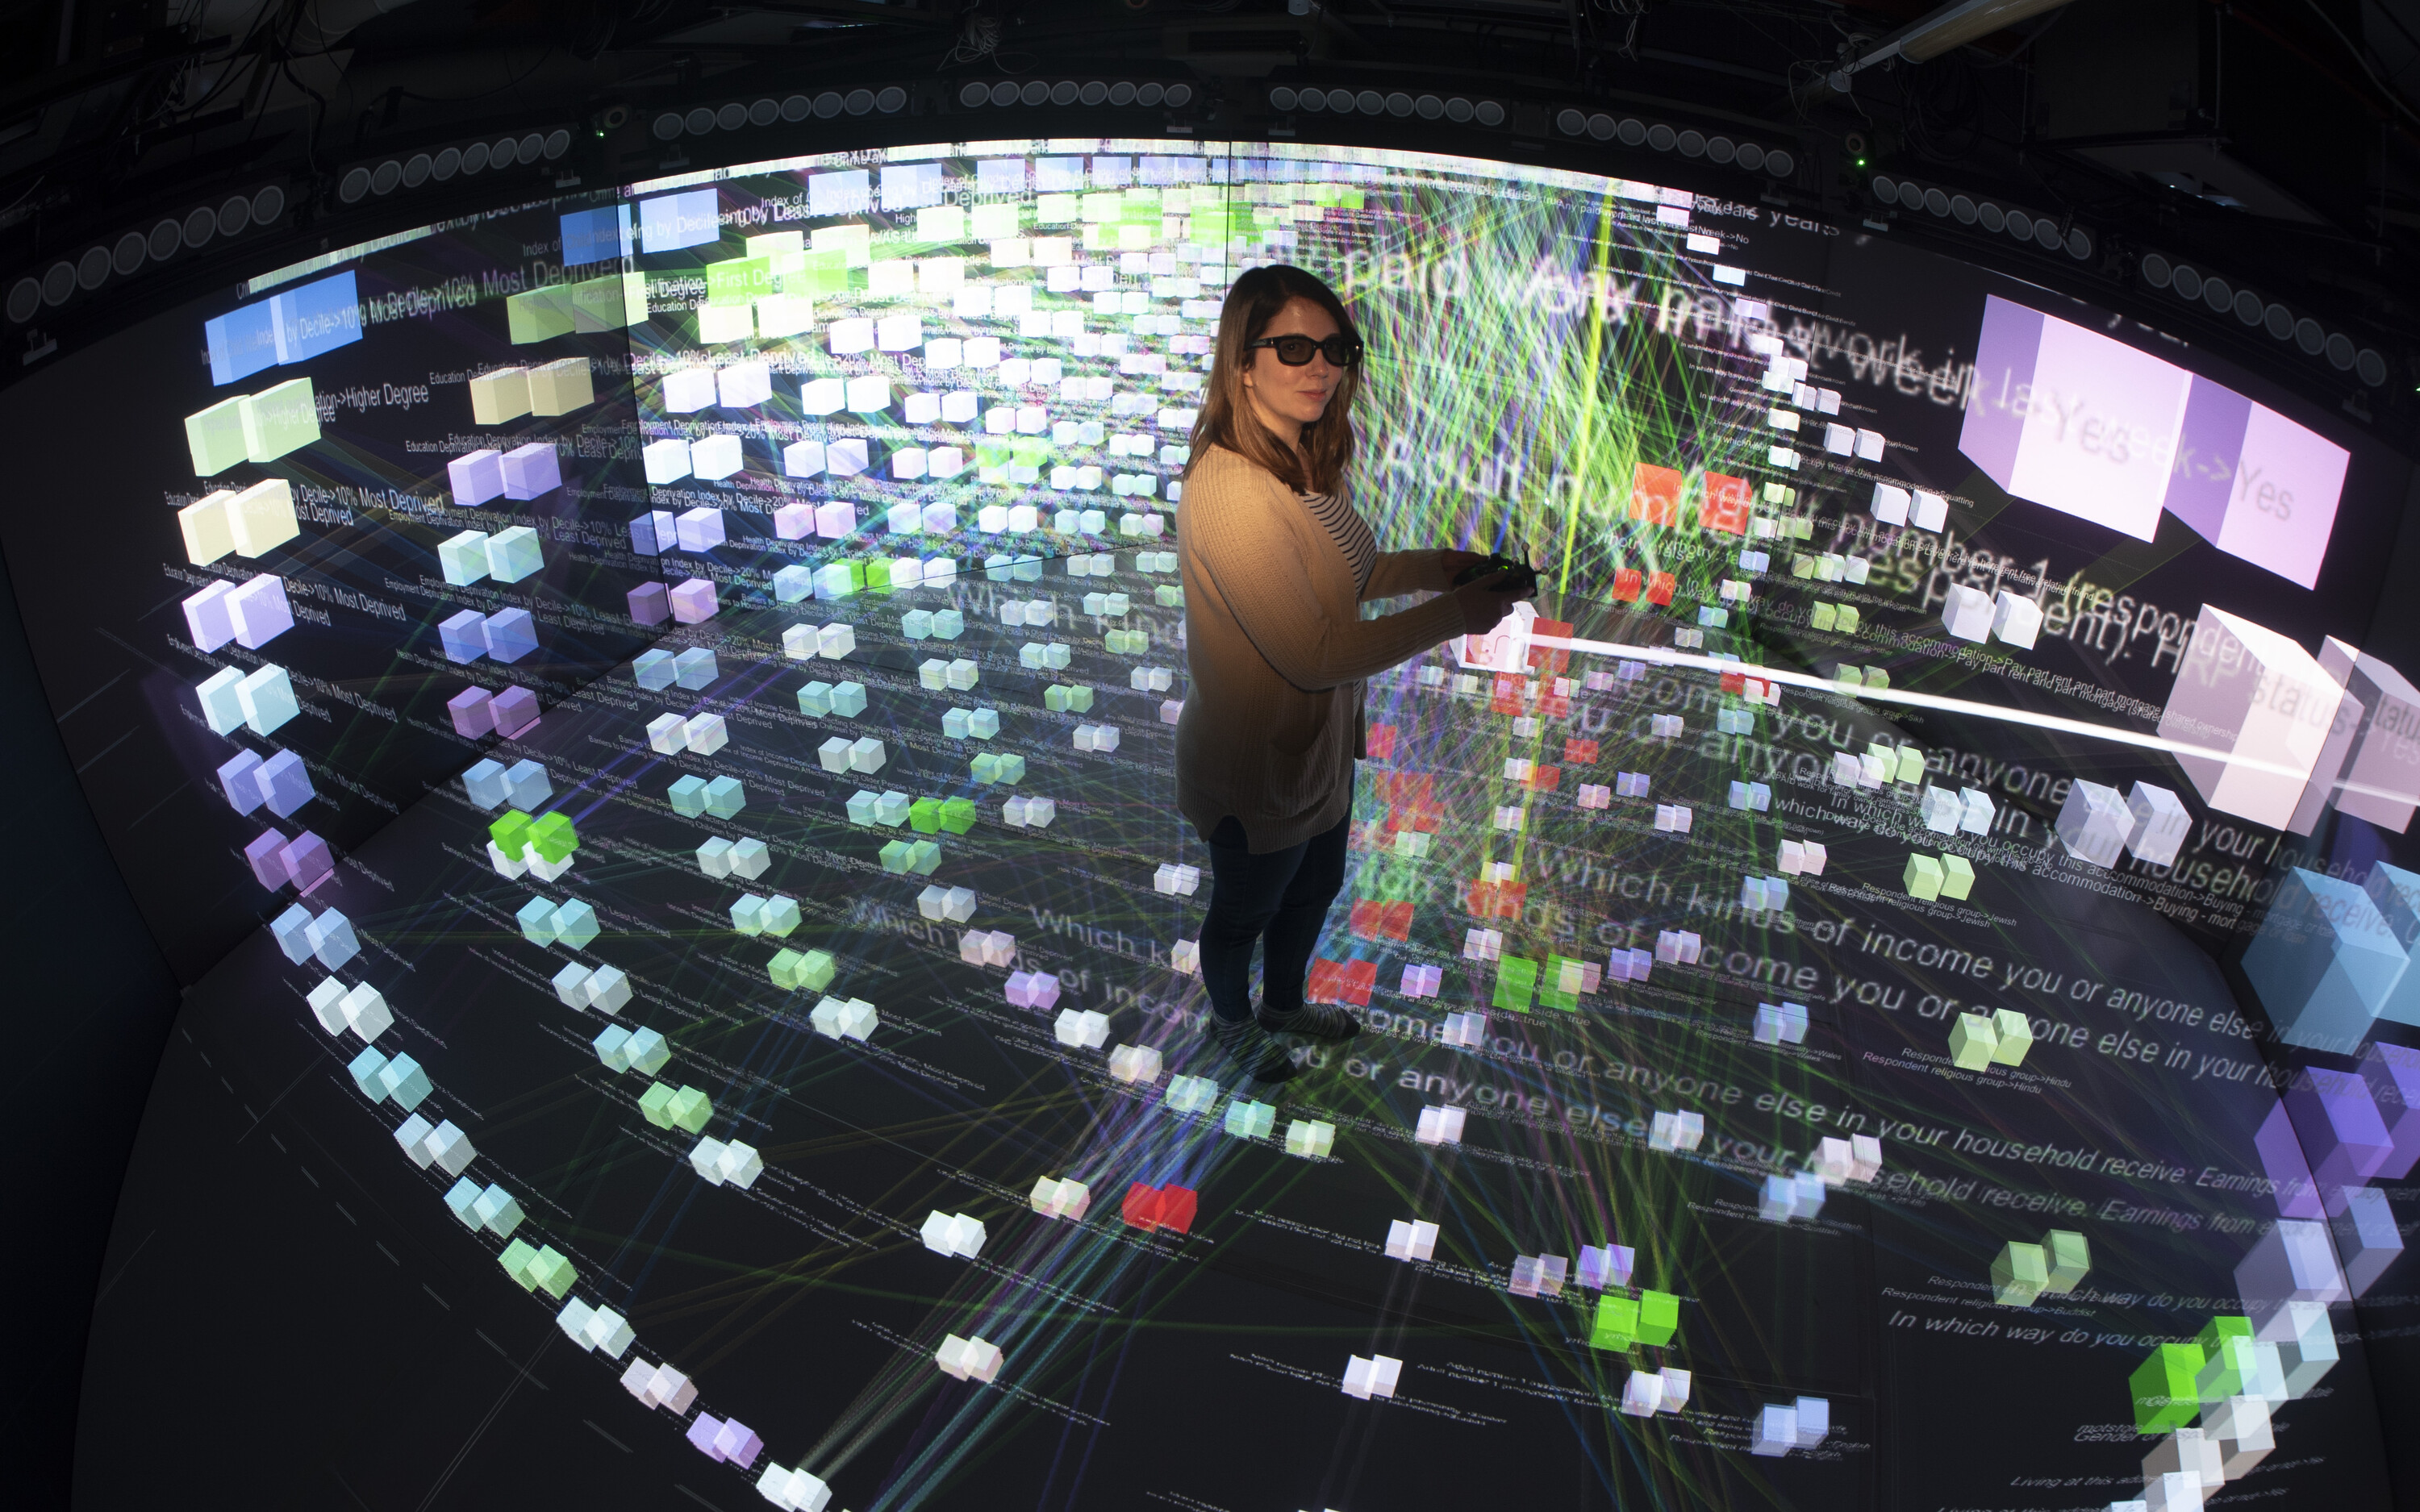
\includegraphics[width=0.92\textwidth]{shot-chloe-octave-2017.jpg}
\caption{Chloe Nevitt interacting with Professor Rob Aspin's unpublished precursor to VisionClaw in the Octave multi-modal laboratory, University of Salford, 2017. Laboratory photograph; the earliest artefact in this system's lineage.}
\label{fig:chloe-octave}
\end{figure}

That heritage came with a platform bet. The 2022 monograph that preceded this report \parencite{OHare2022Convergence} recommended Vircadia as the open substrate for shared virtual worlds, and the ecosystem took the recommendation literally before retiring it; Chapter~\ref{ch:2022-wager} grades that call among the book's cleanest misses and records Vircadia's remnant here as the uninstantiated avatar and presence bridge named later in this chapter. The live surface has moved to the single shared React Three Fiber renderer this chapter verifies below. Naming the migration matters because the shipping documentation kept describing an interim path the code had already left behind, and that kind of espoused-versus-actual drift is exactly what the canon's reconciliation machinery (Chapter~\ref{ch:visionflow-canon}) exists to catch at source.

\begin{figure}[h]
\centering
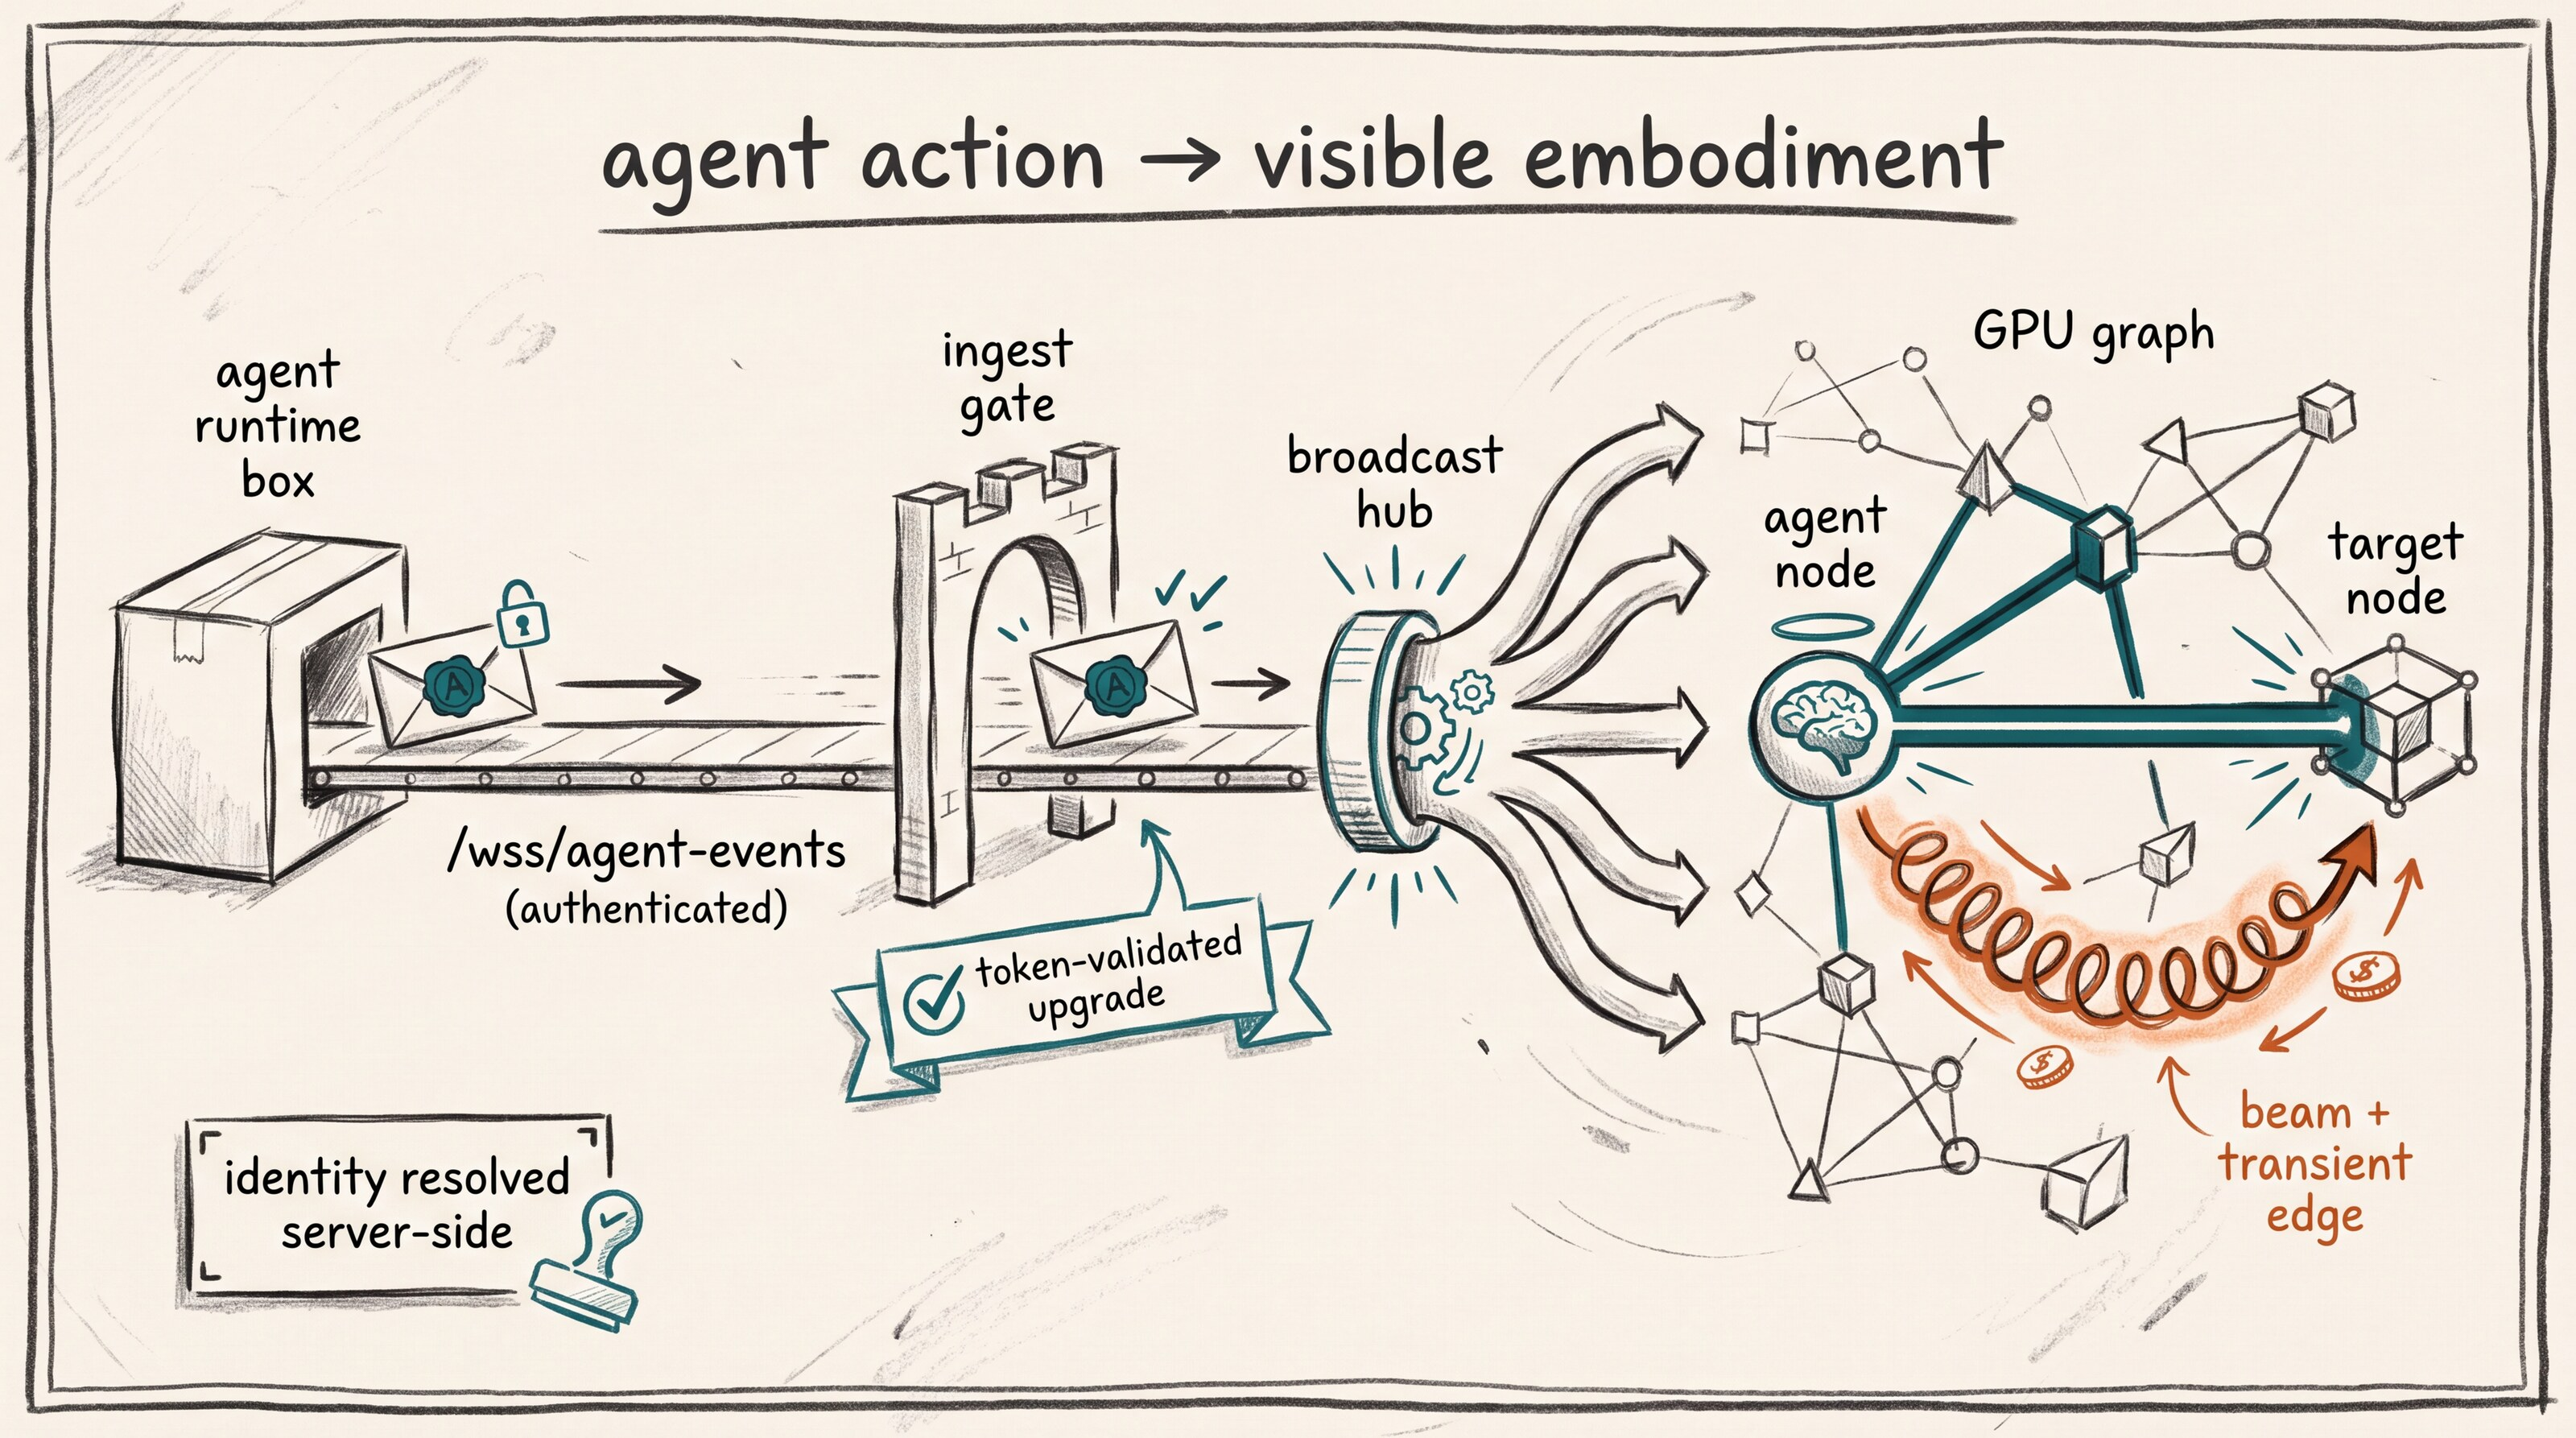
\includegraphics[width=0.95\textwidth]{nb-embodiment-pipeline.jpg}
\caption{VisionClaw's embodiment channel: authenticated \texttt{/wss/agent-events} ingest, hub, beam actor, and client render --- wired end to end, inert at one join (the starved position poll). Illustration in the ecosystem's house sketch style.}
\label{fig:visionclaw-embodiment}
\end{figure}

\section{Watch Here, Judge There}

The ecosystem draws a deliberate line between where agent work is observed and where it is decided. Coordination theory holds that oversight depends on activity being passively and continuously visible in the shared space, and that judgment demands a distinct, deliberate act with the evidence attached. VisionClaw takes the first responsibility and hands the second to the forum. The desktop and headset make agent action legible; the forum makes a human decision cryptographically real. Splitting the two is defensible. It keeps signing authority off the rendering surface, where a stray gesture should never approve anything, and it concentrates the audit trail in one place.

The split carries a cost this edition states plainly. Because the observation surface holds no ambient cue that a judgment case is pending, an escalation raised on the server is invisible to the operator until they leave for the forum. Watching and ruling are correctly separated; they are not yet connected by so much as a badge. Chapter~\ref{ch:gap-register} carries this as a canon omission rather than a mere bug: nothing in the current design gives the surface an operator actually watches a pointer to the surface where a decision waits.

\section{Architecture Stack}

The system comprises five subsystems, each verified against the production codebase.

\subsection{OWL~2 Ontology Engine}

The knowledge graph uses formal OWL~2 ontology via \texttt{horned-owl} and \texttt{whelk-rs} EL inference. The engine parses OWL/XML, Manchester, RDF/XML, and Turtle. This provides shared semantics for agent skill routing: task decomposition uses ontological subsumption rather than keyword matching, so the system treats ``risk assessment'' as a sub-task of ``governance review'' and routes accordingly. Formal ontology gives two properties that informal representations lack: compositionality, so new concepts are constructed from existing ones with guaranteed semantic consistency, and inference, so the system derives relationships that were never stated. These properties make the governance and provenance mechanisms of Chapter~\ref{ch:governance} possible, and the ontology binding of Chapter~\ref{ch:ontology-binding} exposes them to agents at reasoning time.

\subsection{GPU Physics and the Dual Graph}

The visualisation layer runs a Rust/CUDA backend of 82 CUDA kernels for GPU-accelerated graph physics, including clustering, anomaly detection, and PageRank. A published dual-graph demonstration settles 21,038 nodes and 94,702 edges --- a dense knowledge-graph nucleus wrapped in an ontology shell --- under spring, repulsion, and ontology-driven semantic forces in real time. Degree-one dangling wikilink stubs are pruned at ingest, so what settles is navigable structure rather than citation noise.

That is a real advance on the April 2026 position, where production screenshots showed roughly 934 nodes. The 100,000-node-at-60fps figure remains a design target and a unit-test case, not sustained multi-user production load.

\begin{figure}[h]
\centering
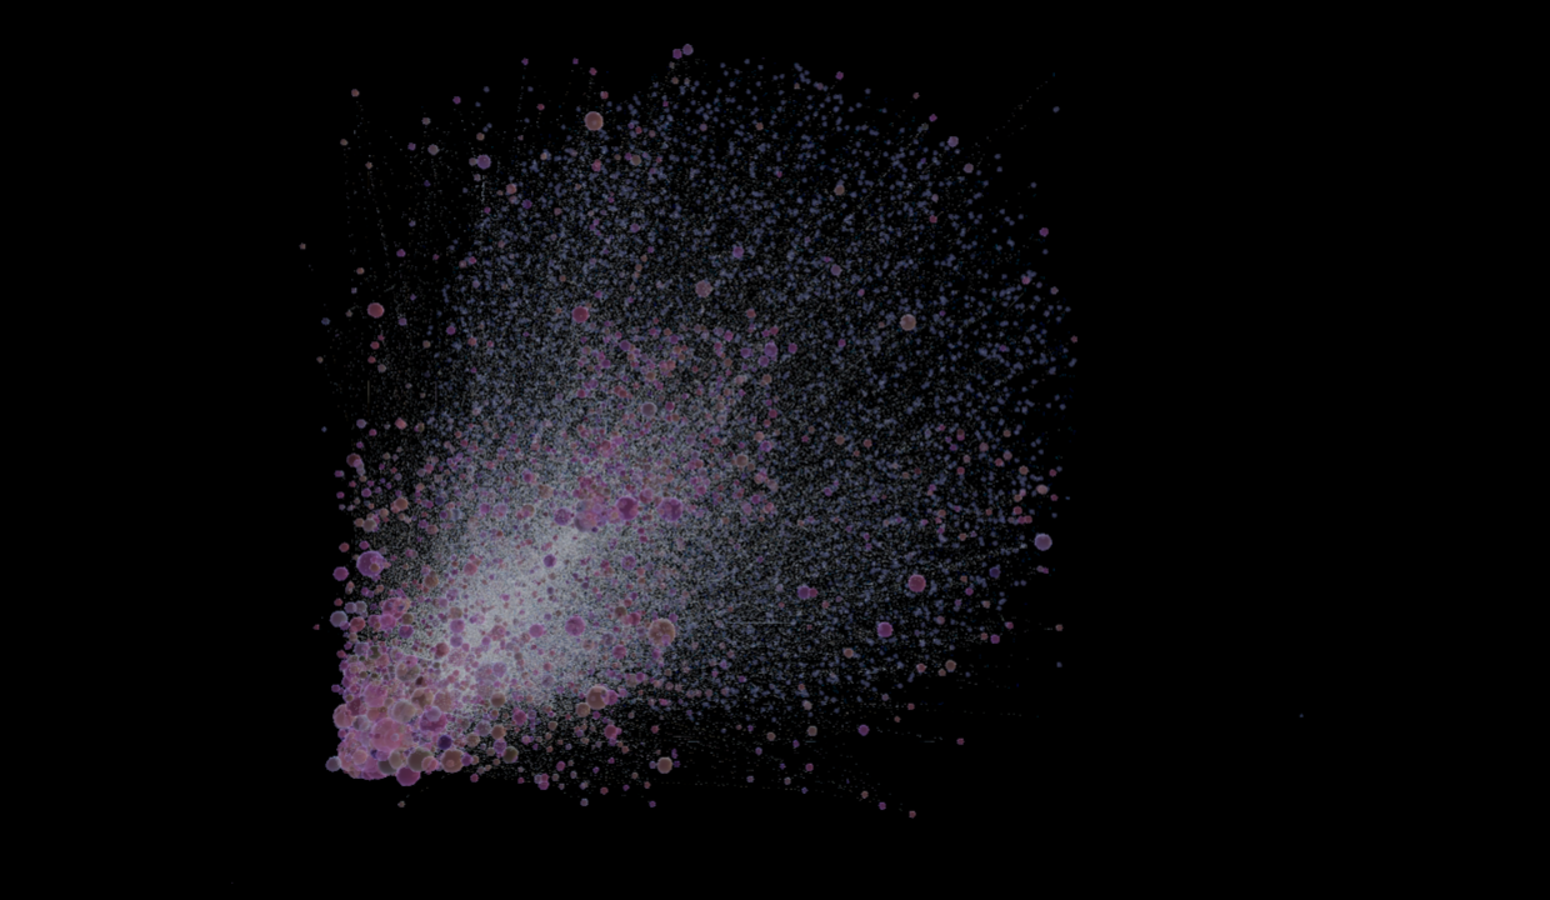
\includegraphics[width=0.95\textwidth]{shot-visionclaw-live.png}
\caption{The live VisionClaw client: GPU-settled knowledge graph with the control surface open. Production screenshot, July 2026.}
\label{fig:visionclaw-live}
\end{figure}

\subsection{WebXR Visualisation}

The client is a single React Three Fiber renderer. The same \texttt{GraphManager} component drives the desktop 2D screen and, wrapped in \texttt{@react-three/xr}, the in-headset view --- shared verbatim rather than duplicated. Earlier documentation described a separate Babylon.js immersive path; the code-verified reality is one shared renderer, which is the stronger engineering position and the one this chapter states. That renderer sits third in a deliberate succession across two technology generations of the same practice: Vircadia, the 2022 platform named above; the Babylon.js path just described, documented but never built as a separate system; and the shared React Three Fiber renderer verified here.

\subsection{Nostr Agent Identity}

Agent and human identities use the Nostr protocol with NIP-98 HTTP authentication. A single \texttt{did:nostr} keypair is the intended universal principal across every trust boundary: relay identity, HTTP auth, provenance author, and DID subject. The design is genuine and ahead of a still-draft industry standard. The gap, examined below and in Chapter~\ref{ch:gap-register}, is that agent nodes on the embodiment surface are still keyed by ephemeral task identifiers, not by their \texttt{did:nostr}, so cryptographic addressing is not yet usable where an operator would select an agent.

\subsection{RuVector Memory}

The persistent memory layer holds over 1.17 million vector embeddings in PostgreSQL with pgvector and HNSW indexing, giving agents memory across sessions. This addresses one of the limitations of Every's agent-colony model, where memory gaps cause context loss between sessions \parencite{Shipper2026}.

\section{Agent Events Reach the Server, Not Yet the Screen}

Since the April 2026 edition, the largest single change to VisionClaw is the agent-events pipe specified in \texttt{ADR-059}. An authenticated \texttt{/wss/agent-events} WebSocket now ingests agent actions from the runtime; a process-global hub fans them to an \texttt{AgentBeamActor}, which broadcasts a compact binary frame that the client decodes into a transient store and renders as a coloured beam from the acting agent to the knowledge node it touched. The beam render actor, listed as entirely missing in the previous edition, has shipped and is wired at boot, and the same code path runs verbatim inside the headset.

A companion \texttt{AcspClient} and \texttt{ElevationActor} dispatcher shipped alongside it: the server genuinely produces kind-31402 broker cases and consumes kind-31403 admin decisions over the forum relay, and a separate \texttt{AgentMonitorActor} live-polls agentbox's management API for real running-task status and lays the agents out in the graph. On paper, the embodiment channel is built.

It does not yet reach the screen. The embodiment channel exists in code, but live agent activity is invisible to the operator, starved by a single unstarted poll rather than by missing infrastructure. The beam's source-position lookup reads \texttt{/api/bots/agents}, an endpoint backed by a polling loop whose only trigger, \texttt{BotsClient::connect()}, is called nowhere in the server bootstrap; the resolver therefore always fails and no beam is ever drawn, and the dedicated agent-avatar layer, reading the same starved endpoint, shows zero agents even while real tasks run.

The live data does exist, one hop away. \texttt{AgentMonitorActor} polls agentbox for genuine task status each cycle and lays the agents out in a golden-angle spiral served at \texttt{/api/bots/data}, but the avatar hook that could consume it extracts only the edges and discards the real node payload. So two independent reasons keep running agents off the screen: a poll that never starts and a consumer that throws away the half it needs. The transient attractive edge --- the ``gluon'' pull the ADR specified --- was retracted in code as infeasible on the current GPU buffer layout and deferred, with the deferral documented honestly at the point of the decision, and the despawn actor the ADR designed was replaced by a simpler client-side expiry the ADR never mentions. The 2026-07-03 closeout marks the beam actor as wired at boot; the code-verified survey shows the transport wired and the live data source unstarted, and this chapter states the second. Chapter~\ref{ch:gap-register} records this as the desktop surface's headline gap and traces the one-line fix.

One further honesty flag belongs here rather than buried in the register. The ``MCP Connected'' status dot on the spawn modal is hardcoded to report connected, never calling the connection test that sits available in the same file, so a down backend still reads as healthy. A status signal decoupled from ground truth miscalibrates trust exactly when intervention is needed, and it is the direct opposite of the honesty the same codebase models in its gluon-deferral comment. The fix is a few lines; the reason to name it is that a fabricated green light on an observation surface is a governance defect, not a cosmetic one.

The re-imagined control centre (\texttt{ADR-129}) is, at present, a settings surface rather than a governance one. It drives per-type node toggles, force parameters, and live connection status, and a natural-language command box dispatches view and physics intents to a real settings assistant. It carries no broker inbox, no approve-or-reject affordance, and no in-scene indicator that a judgment case is pending. An operator watching the graph must leave for the forum to see, let alone decide, anything a human is being asked to rule on. The desktop is deliberately observation-only; the honest consequence is that an escalation the server just raised is invisible on the surface the operator is actually watching.

\section{Immersive WebXR}

In the headset, the working half genuinely works. A user can enter an \texttt{immersive-vr} session, see the live knowledge graph rendered by the same \texttt{GraphManager} the desktop uses, see the live agent nodes, and grab and drag ordinary graph nodes with a controller ray that round-trips real drag events over the WebSocket. The beam pipeline renders in-headset exactly as on the desktop, subject to the same starved-poll caveat above.

Agent interaction does not work. The custom agent-targeting scene never reads a real headset pose, so its selection ray originates at the world origin and finds the right node only by coincidence; the select callback is wired to nothing; hand-tracking sets flags but never a pose; gaze selection is absent. No command panel, agent-detail panel, or ACSP case view is imported anywhere in the immersive tree, so there is no way to inspect, steer, approve, or command an agent from inside mixed reality.

The surface is identity-blind in the same way the desktop is: agent nodes carry no verifiable \texttt{did:nostr}, so a headset user cannot confirm which cryptographic actor produced a beam. Only \texttt{immersive-vr} is reachable in practice; the passthrough \texttt{immersive-ar} path exists as real code but is orphaned from the renderer and disabled by default. A quieter defect sits underneath: the working VR entry never sets the platform's own \texttt{isXRMode} flag, so during a live session the app renders as though it were on the desktop --- a state-model error invisible in documentation and surfacing only on the device. Multi-user copresence sits in the same drawer as the voice binding: an avatar renderer and presence bridge are complete but never connected, so the space is solo by default. Chapter~\ref{ch:gap-register} records the immersive surface's headline gaps as identity-blindness and the absence of any reachable agent-interaction affordance.

\section{Voice}

VisionClaw carries real voice capability, layered and internally uneven. Speech-to-text runs through Whisper-WebUI and text-to-speech through Kokoros, both external services reached over a dedicated speech WebSocket. One loop is fully closed: a \texttt{VoiceInterfaceActor} (\texttt{ADR-110}) subscribes to the transcription stream, matches a conservative verb-and-noun grammar for interface and settings requests, routes them to the same settings assistant the typed command box drives, and confirms the change aloud through Kokoro. A companion \texttt{ElevationActor} harvests spoken concept mentions into a governed elevation ledger, gated off by default.

The step the ecosystem's own design story leads with, speaking to a selected agent, is not consumed. A complete \texttt{PushToTalkService} exists on the client with push and toggle modes and target guarding, but it is imported nowhere in the shipped application, and it has no concept of a selected agent as its target; voice always routes to a generic command pipeline.

A deterministic transcript-to-action producer built in agentbox (\texttt{/v1/voice-intent}) is real and unit-tested but disabled by default and never called by VisionClaw's own speech pipeline; it also has no selection awareness, taking only a flat actor name. Voice is present as capability and closed for settings; the push-to-talk binding to an addressed actor remains built, disabled, and disconnected, and it sits atop the same missing \texttt{did:nostr} keying that blocks addressing an agent anywhere on the surface.

\section{Embodiment Across the Surfaces}

Table~\ref{tab:embodiment-surfaces} summarises the position. Each surface has a genuine working core and a specific thing that does not yet reach the operator, and the pattern is consistent: the infrastructure is present, the last join is not made.

\begin{table}[h]
\centering
\caption{Embodiment state across VisionClaw's surfaces, July 2026}
\label{tab:embodiment-surfaces}
\begin{tabularx}{\textwidth}{L{3.4cm} X L{4.2cm}}
\toprule
\textbf{Surface} & \textbf{What a human can do today} & \textbf{What does not yet reach the operator} \\
\midrule
Desktop 3D (2D screen) & Spawn a real agentbox task; issue view and physics commands; inspect any node & Beams and agent avatars (starved poll); steer, interrupt, or approve in scene; a pending-judgment cue \\
\addlinespace
Immersive WebXR (Quest-class) & Enter \texttt{immersive-vr}; see the live graph and agent nodes; grab and drag nodes & Select or command an agent; verify actor identity; passthrough AR \\
\addlinespace
Voice (Whisper-WebUI, Kokoros) & Speak a settings change and hear it confirmed (\texttt{ADR-110}) & Address a selected agent; voice-to-actor intent binding \\
\addlinespace
Forum (nostr-rust-forum) & Sign a kind-31403 approve or reject decision & By design, judgment lives here, not on the observation surfaces (Chapter~\ref{ch:forum-governance}) \\
\bottomrule
\end{tabularx}
\end{table}

\section{What Is Real and Verified}

Verified against the July 2026 codebase:

\begin{itemize}
  \item OWL~2 reasoning with Whelk-rs EL inference --- functional, and unusual in the agentic space.
  \item GPU-accelerated graph physics across 82 CUDA kernels, with a published dual-graph demonstration settling 21,038 nodes and 94,702 edges in real time.
  \item A single React Three Fiber renderer shared verbatim between desktop and headset, with working \texttt{immersive-vr} entry, live graph, and node manipulation.
  \item Nostr NIP-98 authentication and signing.
  \item The \texttt{ADR-059} agent-events transport, wired ingest-to-render at boot, with its live position source unstarted.
  \item A closed voice-to-settings loop (\texttt{ADR-110}) and a server-side ACSP producer and consumer for the forum's judgment flow.
  \item RuVector memory holding over 1.17 million embeddings with HNSW indexing.
\end{itemize}

\section{What Was Previously Overclaimed}

\begin{cautionbox}[title={Corrected Claims, with Their July 2026 Status}]
An April 2026 codebase audit identified several claims in earlier versions of this document that exceeded what the code supported. The corrections are kept because the history matters; each now carries its July 2026 status.
\begin{itemize}
  \item ``101 specialist skills'' was corrected to a smaller integrated set. \emph{July 2026: the correction stands, but the exact figure is still in motion --- the project README states 88 agent skills while other repositories in the tree report different counts on the same day. Every skill count is a point-in-time snapshot of a fast-moving system.}
  \item Multi-model orchestration via Jarvis, Gemini, and GLM-4 DAG pipelines did not exist; the system used Claude-Flow only. \emph{July 2026: still accurate for VisionClaw. AgentBox now fronts several foundation models, but engineered verification diversity across them is not yet the practice (Chapter~\ref{ch:ecosystem-roadmap}).}
  \item W3C-compliant DID key rotation was not implemented. \emph{July 2026: unchanged. A \texttt{did:nostr} identity spine is designed and intended as the universal principal, yet agent nodes on this surface are still keyed by ephemeral task identifiers, and no W3C DID rotation code exists.}
  \item ``100,000+ nodes at 60fps'' was a unit-test case, not a validated production capability; screenshots showed roughly 934 nodes. \emph{July 2026: materially improved --- the dual-graph demonstration now settles about 21,000 nodes in real time --- but the 100,000-node target and sustained multi-user load at that scale remain unproven.}
  \item ``4M+ tokens of live knowledge graph'' could not be verified. \emph{July 2026: unchanged; 1.17 million vector entries exist, no token-counting infrastructure does.}
  \item ``96GB VRAM --- Dual A6000 Ada'' appeared only in skill examples; the README specified RTX 4080+ (16GB). \emph{July 2026: unchanged; the README still targets RTX 4080-class hardware.}
  \item ``Stratified unidirectional links'' had no supporting code or documentation. \emph{July 2026: unchanged; still not found.}
\end{itemize}
\end{cautionbox}

The corrected picture is still strong. A working OWL~2 plus CUDA plus WebXR plus Nostr plus Claude-Flow substrate, with over a million vector embeddings and a shipped agent-events transport, is genuinely novel at this scale.

It does not need inflation, and the one honest weakness --- that the embodiment channel is wired but starved --- is a single unstarted call away from closing, which is a far more defensible position than a hidden gap would be. The pattern the code review found is consistent across every surface: the hard infrastructure is built, and the failures are joins left unmade, which is the kind of gap a team can close and report against rather than the kind it must quietly explain away.

\section{VisionClaw in Liu's Taxonomy}

Chapter~\ref{ch:coordination-economics} introduced Liu's taxonomy of organisational forms for agent collectives, in which agent-native forms decisively outperform human-imitation ones \parencite{Liu2026}. VisionClaw's subsystems map onto that taxonomy with some precision.

The RuVector memory layer is a blackboard: agents coordinate by reading and writing shared, durable state rather than relaying context through manager agents, the form Liu finds achieves the highest quality of any he tests. Claude-Flow's ontology-grounded routing is a partial adaptive meta-organisation: task decomposition restructures the collective per task, using ontological subsumption as the routing signal, without the explicit contextual-transaction-cost awareness of Liu's orchestrator. The declarative governance layer combined with the judgment broker is an interface organisation: it specifies what may cross from the agentic side into human accountability, and with what evidence attached.

This mapping is interpretive, not measured. Taxonomic resemblance is evidence that the architecture points the right way; it is not evidence that VisionClaw's shared-state coordination pays the context tax at the favourable rates Liu's simulations report. Testing that needs production instrumentation of contextual transaction cost, and the honest position is narrow: the trace plumbing exists, the accounting fields do not, so the measurement Chapter~\ref{ch:ecosystem-roadmap} commits to is close but not yet taken.

\section{Positioning Guidance}

In any external presentation, the following guidelines govern how VisionClaw is described.

\begin{enumerate}
  \item Keep the two names distinct. VisionClaw is the knowledge substrate and embodiment surface described in this chapter; VisionFlow is the umbrella coordination canon (Chapter~\ref{ch:visionflow-canon}). They are not interchangeable, and earlier documents that used them as synonyms were wrong to.
  \item Lead with what is verified. Frame the 100,000-node target, on-screen live embodiment, and multi-provider verification as roadmap items, not current reality.
  \item Position VisionClaw as an existence proof under favourable conditions rather than a proof, honest about the distance between a small technically fluent team and a several-hundred-person firm.
  \item The audience for this document includes people who will check. Overclaiming undermines the genuine strengths of the system and the credibility of the wider argument.
\end{enumerate}

\begin{keyinsight}
The value of VisionClaw to the coordination argument is not that it is the largest or most powerful agentic system. It is that a specific architectural approach --- ontology-grounded orchestration with embedded governance and a designated surface for making agent action visible --- exists in running code. The embodiment channel is built end to end and inert at one join, which is exactly the kind of gap this report insists on naming rather than hiding. A working substrate, even with its beams not yet drawing, moves the argument from ``this could work in theory'' to ``this works in practice, and the remaining question is how far it scales and how fast the last joins close.''
\end{keyinsight}

\chapter{AgentBox: a Sovereign Home for Agents}
\label{ch:agentbox}

\epigraph{An agent you cannot reproduce, audit, or unplug belongs to whoever can. Sovereignty is the standing to say, at any moment, who that is.}{}

\section{Sovereignty as a Governance Property}

The other chapters of Part~\ref{part:visionflow} describe surfaces where a human meets an agent: the forum where a decision gets signed, the desktop where
activity gets watched, the pod where an agent's data lives. AgentBox is the room the agents themselves occupy. It is the container that boots them, hands them
tools, records what they do, and routes their durable writes through identity and redaction before anything reaches storage.
Chapter~\ref{ch:role-transformation} argued that the human's job becomes brokering the judgment agents cannot supply; that job is only defensible if the
operator can see, reproduce, and revoke what the agents actually did. AgentBox exists to make those three verbs true at once.

Sovereignty here is a claim about governance, not about where a server sits. A managed agent platform can run in your own cloud tenancy and still be opaque: you
cannot rebuild its image byte-for-byte, you cannot enumerate every action back to a signing key, and you cannot detach it from the vendor's control plane
without losing your state. AgentBox inverts each of those. The whole environment derives from one \texttt{agentbox.toml} manifest and one Nix flake, producing a
reproducible image; every resource and action is rooted in a cryptographic identity the operator holds; and the runtime is designed to run standalone on a
laptop with local fallbacks, federating into a mesh only when a manifest switch is flipped.

\begin{definitionbox}[title={Sovereignty, operationally}]
An agent runtime is \emph{sovereign} when the operator can independently (1)~\textbf{reproduce} it --- rebuild the exact image from a declared manifest with no
hidden state; (2)~\textbf{audit} it --- attribute every durable write to a signing identity with a provenance trail; and (3)~\textbf{control} it --- run it
disconnected, and revoke or federate it by configuration rather than by permission. Sovereignty is the conjunction. A system that offers any two without the
third leaves the operator dependent on a party they do not govern.
\end{definitionbox}

\section{One Manifest, One Reproducible Image}

Reproducibility is the precondition for the other two properties, because an image you cannot rebuild is an image you cannot audit. AgentBox is built with Nix
flakes, so the manifest that declares which agents, tools, and storage backends are present also fixes the bytes of the resulting container. Capabilities absent
from \texttt{agentbox.toml} add nothing to the image; enabling one gates both its package set and its supervised service block together, so there is no drift
between what the manifest claims and what the container runs. One residual runtime-fetch path remains, a small set of \texttt{npx -y} CLI aliases pending
subresource-integrity pinning, and the documentation names it rather than hiding it, which is the posture the whole report asks of its own systems.

The security posture is stated in \texttt{ADR-027} and is deliberately conservative: the container runs as non-root (uid~1000) with a read-only root filesystem,
\texttt{cap\_drop:~ALL}, \texttt{no-new-privileges:true}, and a supplemental seccomp denylist of forty-seven high-risk syscalls layered on Docker's default
profile. That denylist is honestly labelled a supplement, not a replacement allowlist; the container runtime remains the security boundary. Published ports bind
host-loopback only. None of this is exotic, and that is the point. A sovereign home is built from ordinary, inspectable hardening rather than a bespoke sandbox
nobody else can reason about.

Identity is the spine that makes auditing possible. At bootstrap AgentBox generates a BIP-340 secp256k1 keypair whose public key becomes a \texttt{did:nostr}
identity, and every resource, action, and event roots in it through an eighteen-kind \texttt{urn:agentbox:} grammar minted in one place
(\texttt{management-api/lib/uris.js}). Owner-scoped identifiers embed the hex pubkey, so a credential or an activity record names the agent that issued it and
no other. Beneath the identity layer, the pod substrate described in Chapter~\ref{ch:solid-pod} makes provenance the default: since the
\texttt{solid-pod-rs}~0.5.0 provenance release every pod write lands as a git-mark (a commit plus a PROV-O sidecar recording who wrote what, when), and
high-value or disputed records can escalate to hash-chained block-trails with an optional Bitcoin anchor. Traceability scales from free to settlement-grade per
record, which is the material form of ``audit'' in the definition above.

Table~\ref{tab:agentbox-sovereignty} sets each sovereignty property against the mechanism that delivers it, and against an honest maturity read in the governed
vocabulary of \texttt{ADR-002}. Two rows are staged rather than shipped, and this chapter says so where they appear.

\begin{table}[h]
\centering \caption{AgentBox against the three sovereignty properties}
\label{tab:agentbox-sovereignty}
\begin{tabularx}{\textwidth}{L{2.7cm} X L{2.4cm}}
\toprule
\textbf{Property} & \textbf{Mechanism in AgentBox} & \textbf{Maturity} \\
\midrule
Reproduce & Nix flake plus \texttt{agentbox.toml} manifest; package and service blocks gated together; one \texttt{npx} runtime-fetch path pending SRI pinning & Integrated \\
\addlinespace
Audit & \texttt{did:nostr} identity root; eighteen-kind \texttt{urn:agentbox} grammar; per-write git-marks with PROV-O sidecars; opt-in block-trails & Integrated \\
\addlinespace
Control: disconnect & Five pluggable adapters resolving to local, external, or off; standalone (SQLite plus local JSONL) or federated by manifest switch & Integrated \\
\addlinespace
Control: disclose & Per-slot privacy filter (strict for memory and pods) before durable writes; NIP-59 session mirror sealed to the operator alone & Integrated \\
\addlinespace
Learn from outcomes & Trajectory producer live; \texttt{feed\_retrieval} and \texttt{feed\_routing} consumers corpus-gated off & Scaffolded \\
\addlinespace
Engineered diversity & Four model families fronted; independent-model verification routing available but not enforced & Scaffolded \\
\bottomrule
\end{tabularx}
\end{table}

The two ``control'' rows earn a sentence each, because they are where sovereignty stops being a slogan. Disconnection is real: five adapter slots (beads, pods,
memory, events, orchestrator) each resolve to a local implementation, an external one, or off, so a manifest set to \texttt{standalone} ships a complete product
with local fallbacks and the same image federates into a mesh by flipping one switch to \texttt{client}. Disclosure is enforced in the write path: an embedded
privacy filter (\texttt{ADR-008}) sits in the adapter dispatch, redacting PII and secrets before durable writes reach memory or pods, under a per-slot policy
that is strict and fail-closed for memory and pods, soft for events and beads, and off for the orchestrator control plane. The honest boundary is stated in the
same decision record: the filter is not a universal interceptor on every tool call, so ``redacted before storage'' is a claim about the durable-write slots, not
about the whole runtime.

\section{Skills, and Three Counts in One Tree}

Agents in AgentBox reach their tools through skills: manifest-gated capability bundles, each a directory carrying a \texttt{SKILL.md} contract, routed to the
model through the Model Context Protocol. They cover browser automation via the external sidecar, three-dimensional rendering, geospatial analysis, document
typesetting, a payment router, and a source-grounded knowledge corpus, among others. A skill absent from the manifest costs the image nothing, so the routing
surface is both large and gated.

How large is a fair question, and the honest answer is a small cautionary tale about the difference between a document and a fact. On one day in July~2026, a
single checkout of the repository advertised the skill count three different ways: the top-level \texttt{README.md} said ``90+ skills'', the documentation hub
said ``113 skills'', and the filesystem held 115 directories carrying a \texttt{SKILL.md}. All three were written in good faith; none was a lie; and no two
agreed. The verifiable count is the one you can enumerate, 115, and the two prose figures are a rounded floor and a stale snapshot respectively. This report
treats that drift as instructive rather than embarrassing. A reproducible image guarantees that the tree is identical everywhere, and it guarantees nothing
about whether the prose describing the tree kept pace with it. The skill \emph{routing} is sovereign; the skill \emph{count} in the docs was merely approximate,
and the gap between those two claims is exactly the kind of thing an honest audit surfaces and a marketing page conceals.

\begin{figure}[h]
\centering
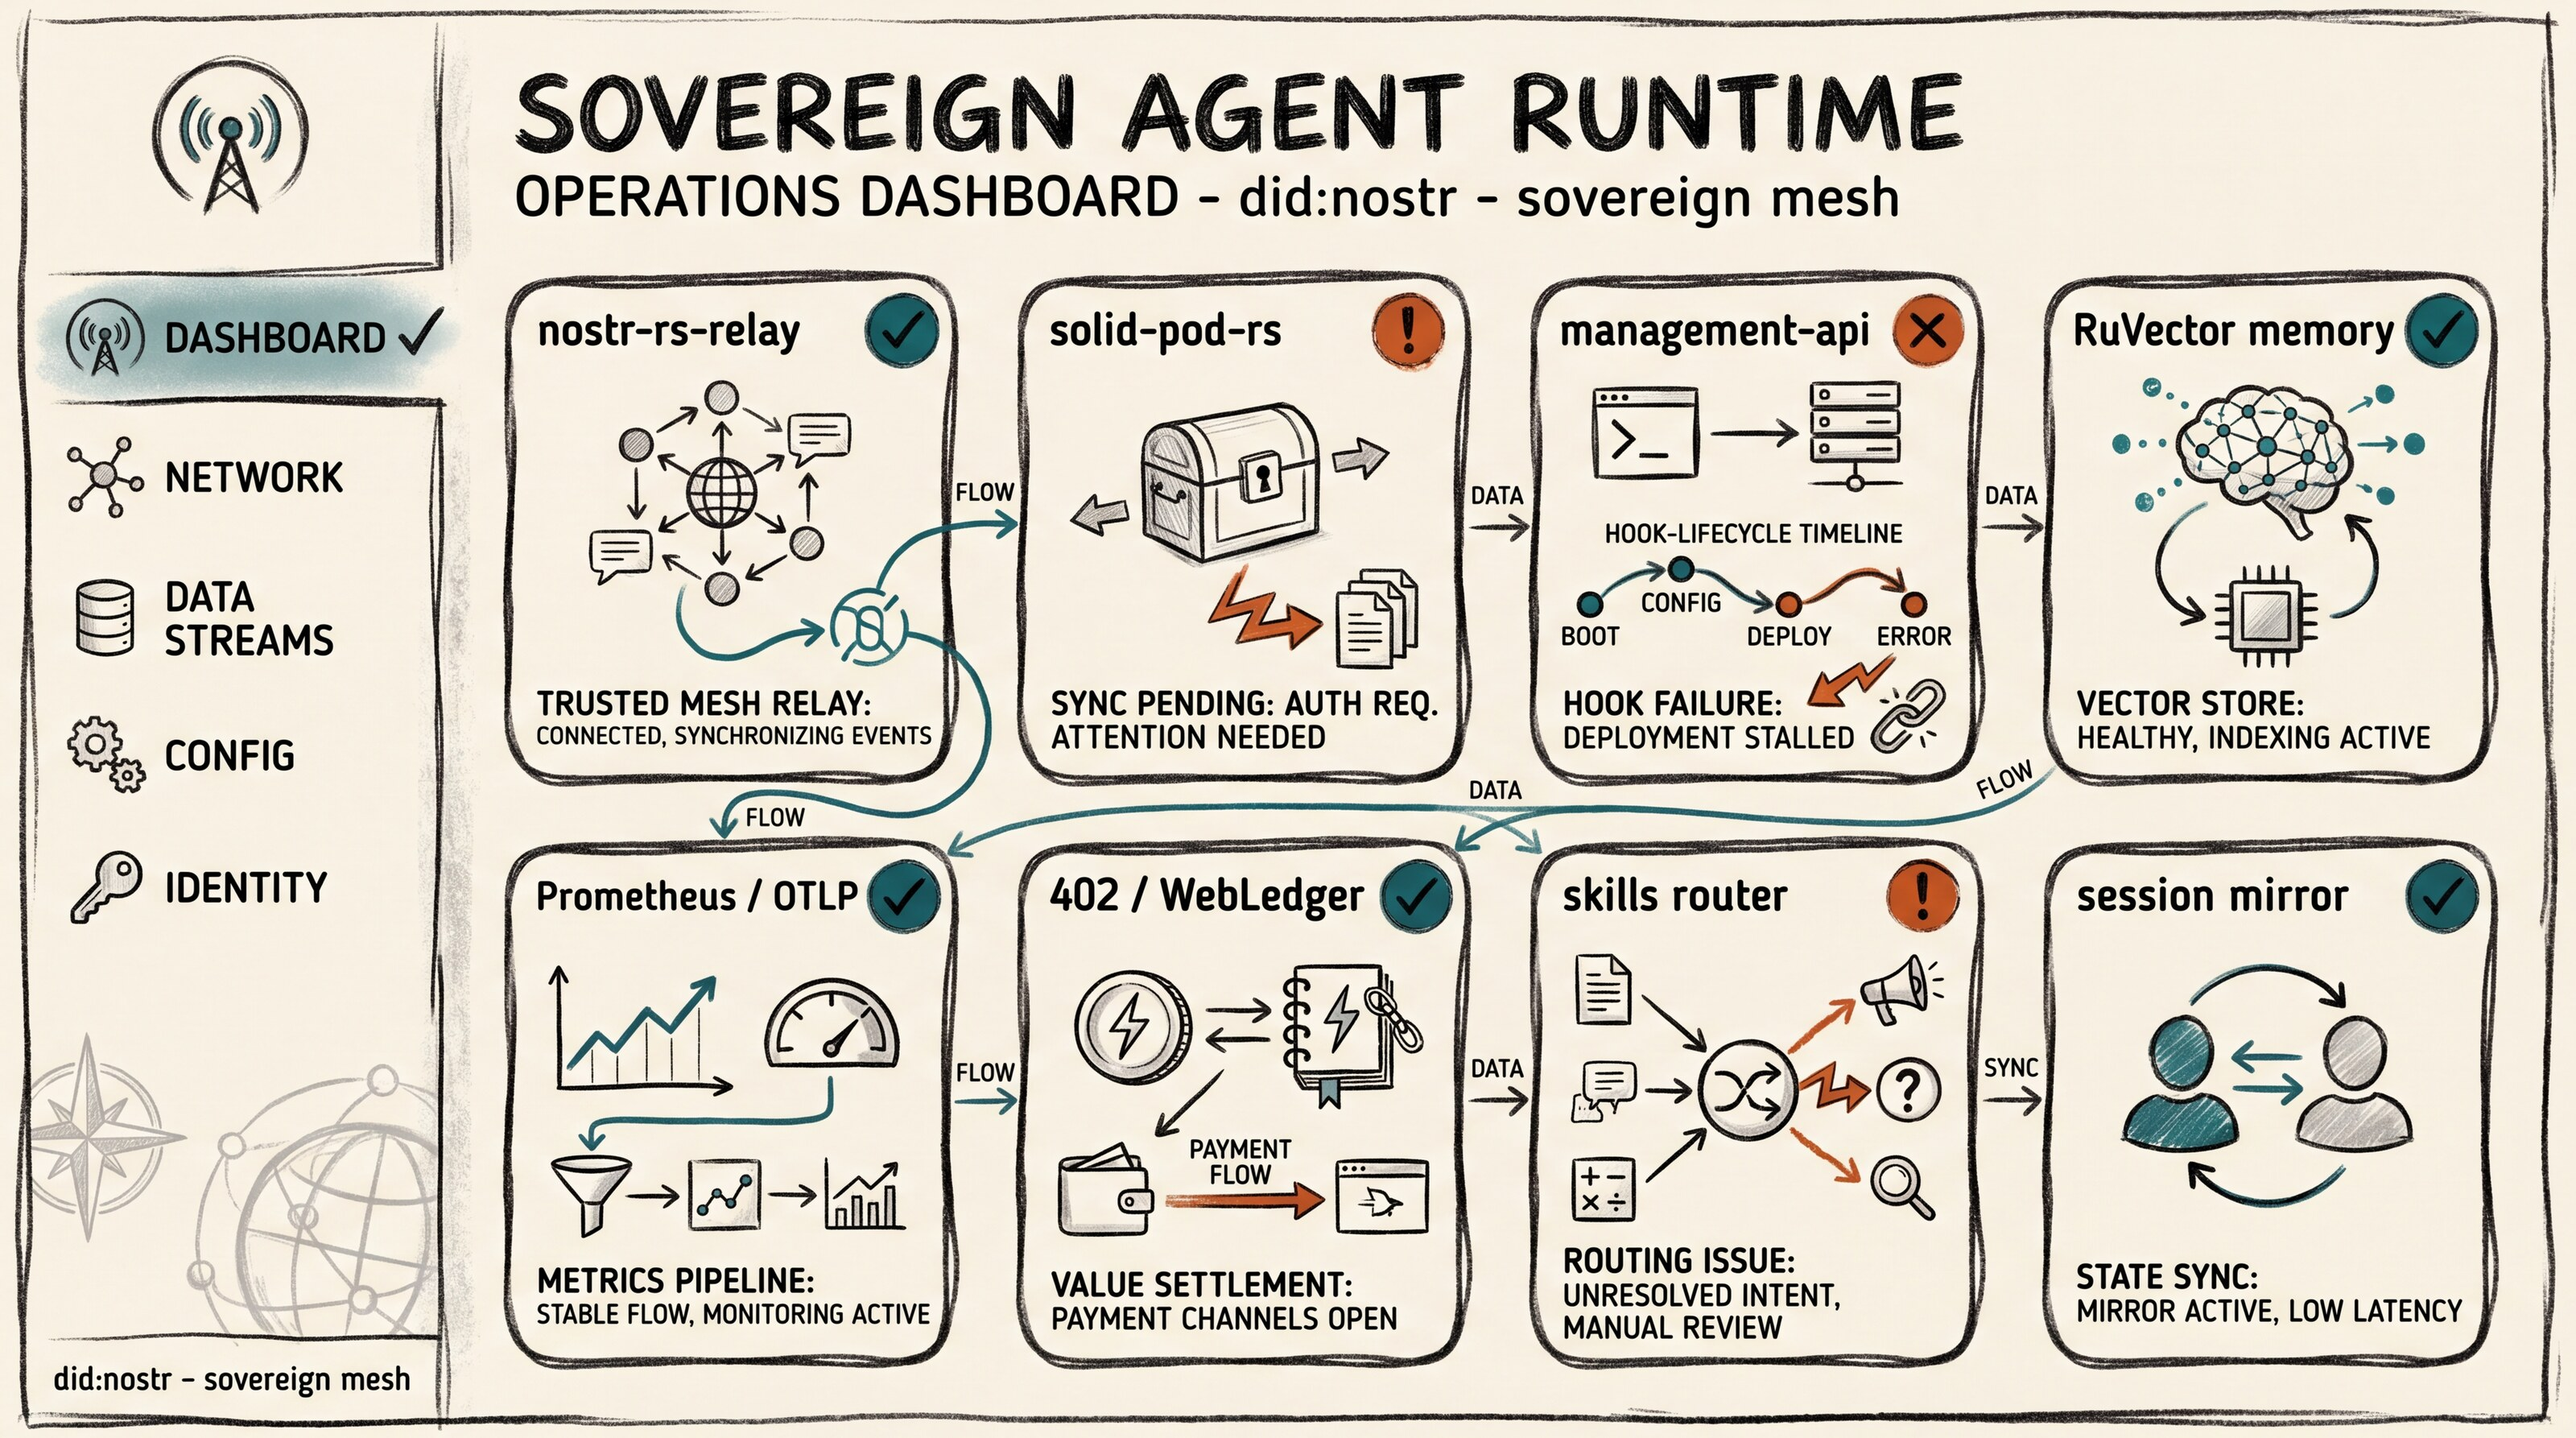
\includegraphics[width=0.92\textwidth]{nb-agentbox-dashboard.jpg}
\caption{The AgentBox operations surface: manifest-gated services with live status, rooted in the operator's \texttt{did:nostr} identity. Illustration in the house sketch style.}
\label{fig:agentbox-dashboard}
\end{figure}

\section{Hooks as a Telemetry Spine}

Every stage of an agent's lifecycle fires a hook. AgentBox registers handlers on \texttt{SessionStart}, \texttt{UserPromptSubmit}, \texttt{PreToolUse},
\texttt{PostToolUse}, \texttt{SubagentStop}, \texttt{Stop}, and \texttt{SessionEnd}, and these are where grounding directives get injected, sessions get
mirrored, and trajectories get recorded. The surface is fail-open by enforced convention: any hook that errors is expected to exit zero and never block the
model. ``Enforced convention'' is a precise and slightly uncomfortable phrase. The guarantee lives in code review and handler discipline, not in a runtime that
sandboxes a misbehaving hook, so the fail-open property is a promise the maintainers keep rather than one the platform imposes.

This spine is where the coordination economics of Chapter~\ref{ch:coordination-economics} would become measurable. \textcite{Liu2026} formalises the contextual
transaction cost that coordination between agents imposes: the handoffs, the compression loss at each boundary, the verification burden. A collective's
efficiency is governed by that cost rather than by any single agent's capability. The \texttt{PostToolUse} and \texttt{SubagentStop} hooks see every handoff and
every verification outcome as they happen, which makes them the natural place to record a contextual-transaction-cost figure per workflow. The instrumentation
is not yet wired: the July~2026 audit found that the one hook seam where a tool outcome could be observed, the \texttt{post-bash} case, currently falls through
to a bare log line and touches nothing. The plumbing exists; the accounting does not. Recommendation~3 of Chapter~\ref{ch:ecosystem-roadmap} commits to closing
that gap and to reporting the first production contextual-transaction-cost figure the framework has, and the same spine is the right place to tag failures to
the fourteen-mode taxonomy of \parencite{Cemri2025} instead of to free-text error strings.

\section{Memory That Must Embed to Exist}

Durable agent memory lives in RuVector, a Postgres sidecar with a genuine vector extension. Writes go through the \texttt{memory\_store} MCP tool, which
computes a 384-dimension embedding client-side via Xinference (model \texttt{bge-small-en-v1.5}, not the MiniLM that older architecture decision records
claimed) and inserts the vector directly; reads go through \texttt{memory\_search} over an HNSW index with SIMD acceleration confirmed active. The store holds
over 1.17~million embeddings. The 2026-07-04 audit counted roughly two million rows in all, most of them frozen legacy telemetry that is written and never read
back, a reminder that corpus size and useful corpus are different measurements.

\begin{keyinsight}[title={The pipeline is the contract}]
An entry with no embedding is invisible to search. HNSW retrieval walks vectors, so a row inserted by raw SQL that skips the embedding step is present in the
table, counted in the totals, and unreachable by every agent that will ever look for it. The audit found 429 such null-embedding rows, sixteen of them raw-SQL
bypasses as recent as June~2026: the exact anti-pattern the workspace conventions warn against, recurring in practice. The rule that follows is not a
preference. Write through \texttt{memory\_store} or do not write, because the embedding pipeline, and not the table, is where a memory becomes a memory.
\end{keyinsight}

The store is strong and the retrieval is real. What the store does not yet do is learn, and this is the chapter's load-bearing correction, because the
compounding organisation of Chapter~\ref{ch:compounding-org} is a claim about closed loops, and a loop that does not close compounds nothing.

\begin{cautionbox}[title={What the memory system does not do yet}]
Three advertised behaviours do not run as described, verified against live code and the live database:
\begin{itemize}
  \item The session-start ``\texttt{[INTELLIGENCE]}'' banner ranks memory by text relevance,
a blend of trigram similarity and PageRank over the local \texttt{MEMORY.md} index. It is useful relevance surfacing. It is text similarity, not outcome
learning, and it never touches Postgres.
  \item The router's ``Confidence: 80\%'' figure is a hardcoded constant:
literal \texttt{0.8} on a regex match, \texttt{0.5} otherwise. No state is read or written to produce it.
  \item Trajectory recording of graded outcomes landed on 5~July~2026:
\texttt{config/hooks/trajectory-recorder.cjs} writes real trajectories and the producer gate is live. The two consumers that would let those outcomes influence
retrieval and routing, \texttt{feed\_retrieval} and \texttt{feed\_routing}, remain gated off until the trajectory corpus clears a statistical sample floor.
\end{itemize}
The remediation is scheduled honestly rather than claimed as done. Recommendation~7 of Chapter~\ref{ch:ecosystem-roadmap} tracks it, and
Chapter~\ref{ch:gap-register} places it in the systematic register; this chapter names the gap once and points there rather than restating the whole account.
\end{cautionbox}

\section{A Whole Session in the Operator's Pocket}

Auditability is worthless if the audit trail lives somewhere the operator never looks. AgentBox mirrors every running session to the operator's phone. A hook
(\texttt{config/hooks/nostr-live-mirror.cjs}) emits one message per turn: the user's prompt on \texttt{UserPromptSubmit}, the assistant's last message on
\texttt{Stop}, and lifecycle markers on \texttt{SessionStart} and \texttt{SessionEnd}. Each is a NIP-59 gift-wrapped self-message, a kind-1059 wrap around a
kind-14 direct-message rumour, end-to-end sealed to the operator's own key, with the encrypted wrap to the cloud relay as the only network egress. In any Nostr
client the session reads as a single note-to-self thread that only the recipient key can decrypt, and the relay gates reads behind authentication.

The design choices matter for sovereignty. The message stream is sealed to a key the operator holds, not to a vendor dashboard; the recipient is a key derived
from the operator's root identity, so the root secret never leaves the container; and the whole mechanism is a silent no-op when no recipient pubkey is
configured, so it discloses to exactly one party by construction. A curated end-of-session digest (a kind-30840 summary) rides the same spine as the slower,
edited sibling of the per-turn stream. Together they give the operator two views of what their agents did, the live feed and the retrospective, on a device they
carry, sealed to a key they control. Recommendation~9 of Chapter~\ref{ch:ecosystem-roadmap} extends this so that an escalated decision reaches the phone
carrying its evidence and uncertainty, not merely its conclusion, which is what \textcite{Liu2026}'s interface-organisation specification requires of any
uncertainty disclosure.

\section{Multi-Model Fronting and Engineered Diversity}

AgentBox fronts four foundation-model families out of the box (Claude, Codex, Gemini, and DeepSeek) plus a meta-router for named external consultations. This is
the plumbing for a specific and easily-missed requirement from the coordination literature. \textcite{Liu2026} shows that diversity in an agent collective must
be engineered rather than assumed: a reviewer drawn from the reviewed agent's own model family, running the same tools over the same retrieval, is one judge
asked three times. Genuine verification needs independent models with independent evidence paths.

The plumbing being present is a weaker fact than the discipline being practised, and this report will not conflate them. Fronting four models makes it possible
to route a verification agent to a different family than the one that produced the work; nothing in the current configuration requires it. Recommendation~8 of
Chapter~\ref{ch:ecosystem-roadmap} names the gap and commits to routing critique and verification agents onto foundations independent of the agent under review.
The distinction is the one this part of the book keeps returning to: capability in the substrate is a precondition for the behaviour and never a replacement for
it.

\section{What Is Solid, and What Is Staged}

AgentBox is the most operationally mature component of the ecosystem. The runtime, the identity spine, the reproducible build, the secure posture, the memory
store, and the session mirror are integrated and running, and the memory-and-learning workstream (\texttt{PRD-018}) landed in production in early July~2026. Two
things are honestly staged rather than shipped. The learning loop records outcomes and does not yet consume them, so ``memory that compounds'' remains a
scheduled property rather than a demonstrated one. Multi-model verification is available and not enforced, so ``engineered diversity'' is a capability awaiting
a discipline. Both gaps are entered in the register of Chapter~\ref{ch:gap-register} and carry dated commitments in Chapter~\ref{ch:ecosystem-roadmap}. A
sovereign home for agents is worth building while parts of it are still under construction, provided the building notices which rooms are finished and says so
out loud. The proprietary trace an agentic system accumulates is its durable advantage \parencite{Pereira2026Playbook}, and a trace is only an advantage if
every write that composes it is attributable, reproducible, and reachable. That is the whole case for giving agents a home you govern.

\chapter{solid-pod-rs: Data That Belongs to Its Actor}
\label{ch:solid-pod}

\epigraph{The exit right has to sit in the floor, not be granted at the door.}{}

\section{Why Every Actor Needs a Pod}

Part~\ref{part:problem} diagnosed hierarchy as an information-routing protocol and showed how AI collapses the cost of the routing function that hierarchy was built to serve. A quieter claim sits underneath that diagnosis, and it becomes load-bearing the moment collaboration crosses an organisational boundary: the platforms that host today's collaboration scale tokens, not trust.

A centralised system can hand out a billion API credentials in an afternoon. What it cannot manufacture is a counterparty's justified confidence that its data will not be read, retained, retrained on, or held hostage by the platform operator. Trust of that kind does not come from the platform. It comes from the counterparty being able to leave with everything that is theirs, at any time, without asking.

solid-pod-rs is DreamLab's answer to that constraint: a place where every actor's data lives under the actor's own cryptographic control, portable by construction. In the ecosystem's division of labour (Chapter~\ref{ch:ecosystem-roadmap}) it is the sovereign data layer, the canonical store the other components read from and write to. The design commitment is uniform across the human/agent line. A person gets a pod, and so does each agent, each rooted in the same \texttt{did:nostr} identity it uses everywhere else in the mesh. Storage is the actor's own, and access to it is decided by the actor's own key, rather than a service an operator grants and may withdraw.

The exit right this produces is structural rather than contractual. Leaving the mesh is not a data-export request that an operator may slow-walk or deny. It is the actor already holding the keys to storage that was theirs the whole time. That property is the trust precondition for collaboration between organisations that do not, and need not, trust each other's infrastructure. It is also the precondition for the data moat that Chapter~\ref{ch:compounding-org} argues for: the durable, provenance-carrying record that \textcite{Pereira2026Playbook} found 47~per~cent of successful deployments citing as their defensible asset is only an asset if its owner cannot be separated from it.

The interface-organisation model that \textcite{Liu2026} places at the centre of agent-collective efficiency needs a data layer it does not itself describe. An interface organisation connects an agent's context to a human's accountability across a boundary, and it can do so only if both the context and the accountability attach to principals each side can verify without trusting the other's servers. A pod supplies exactly that. The agent's evidence lives under an addressable, signed identity; the human's decision is recorded against storage the human controls; and coordination across organisational lines then rests on cryptography both parties can check rather than on a shared operator both parties must trust.

\begin{figure}[h]
\centering
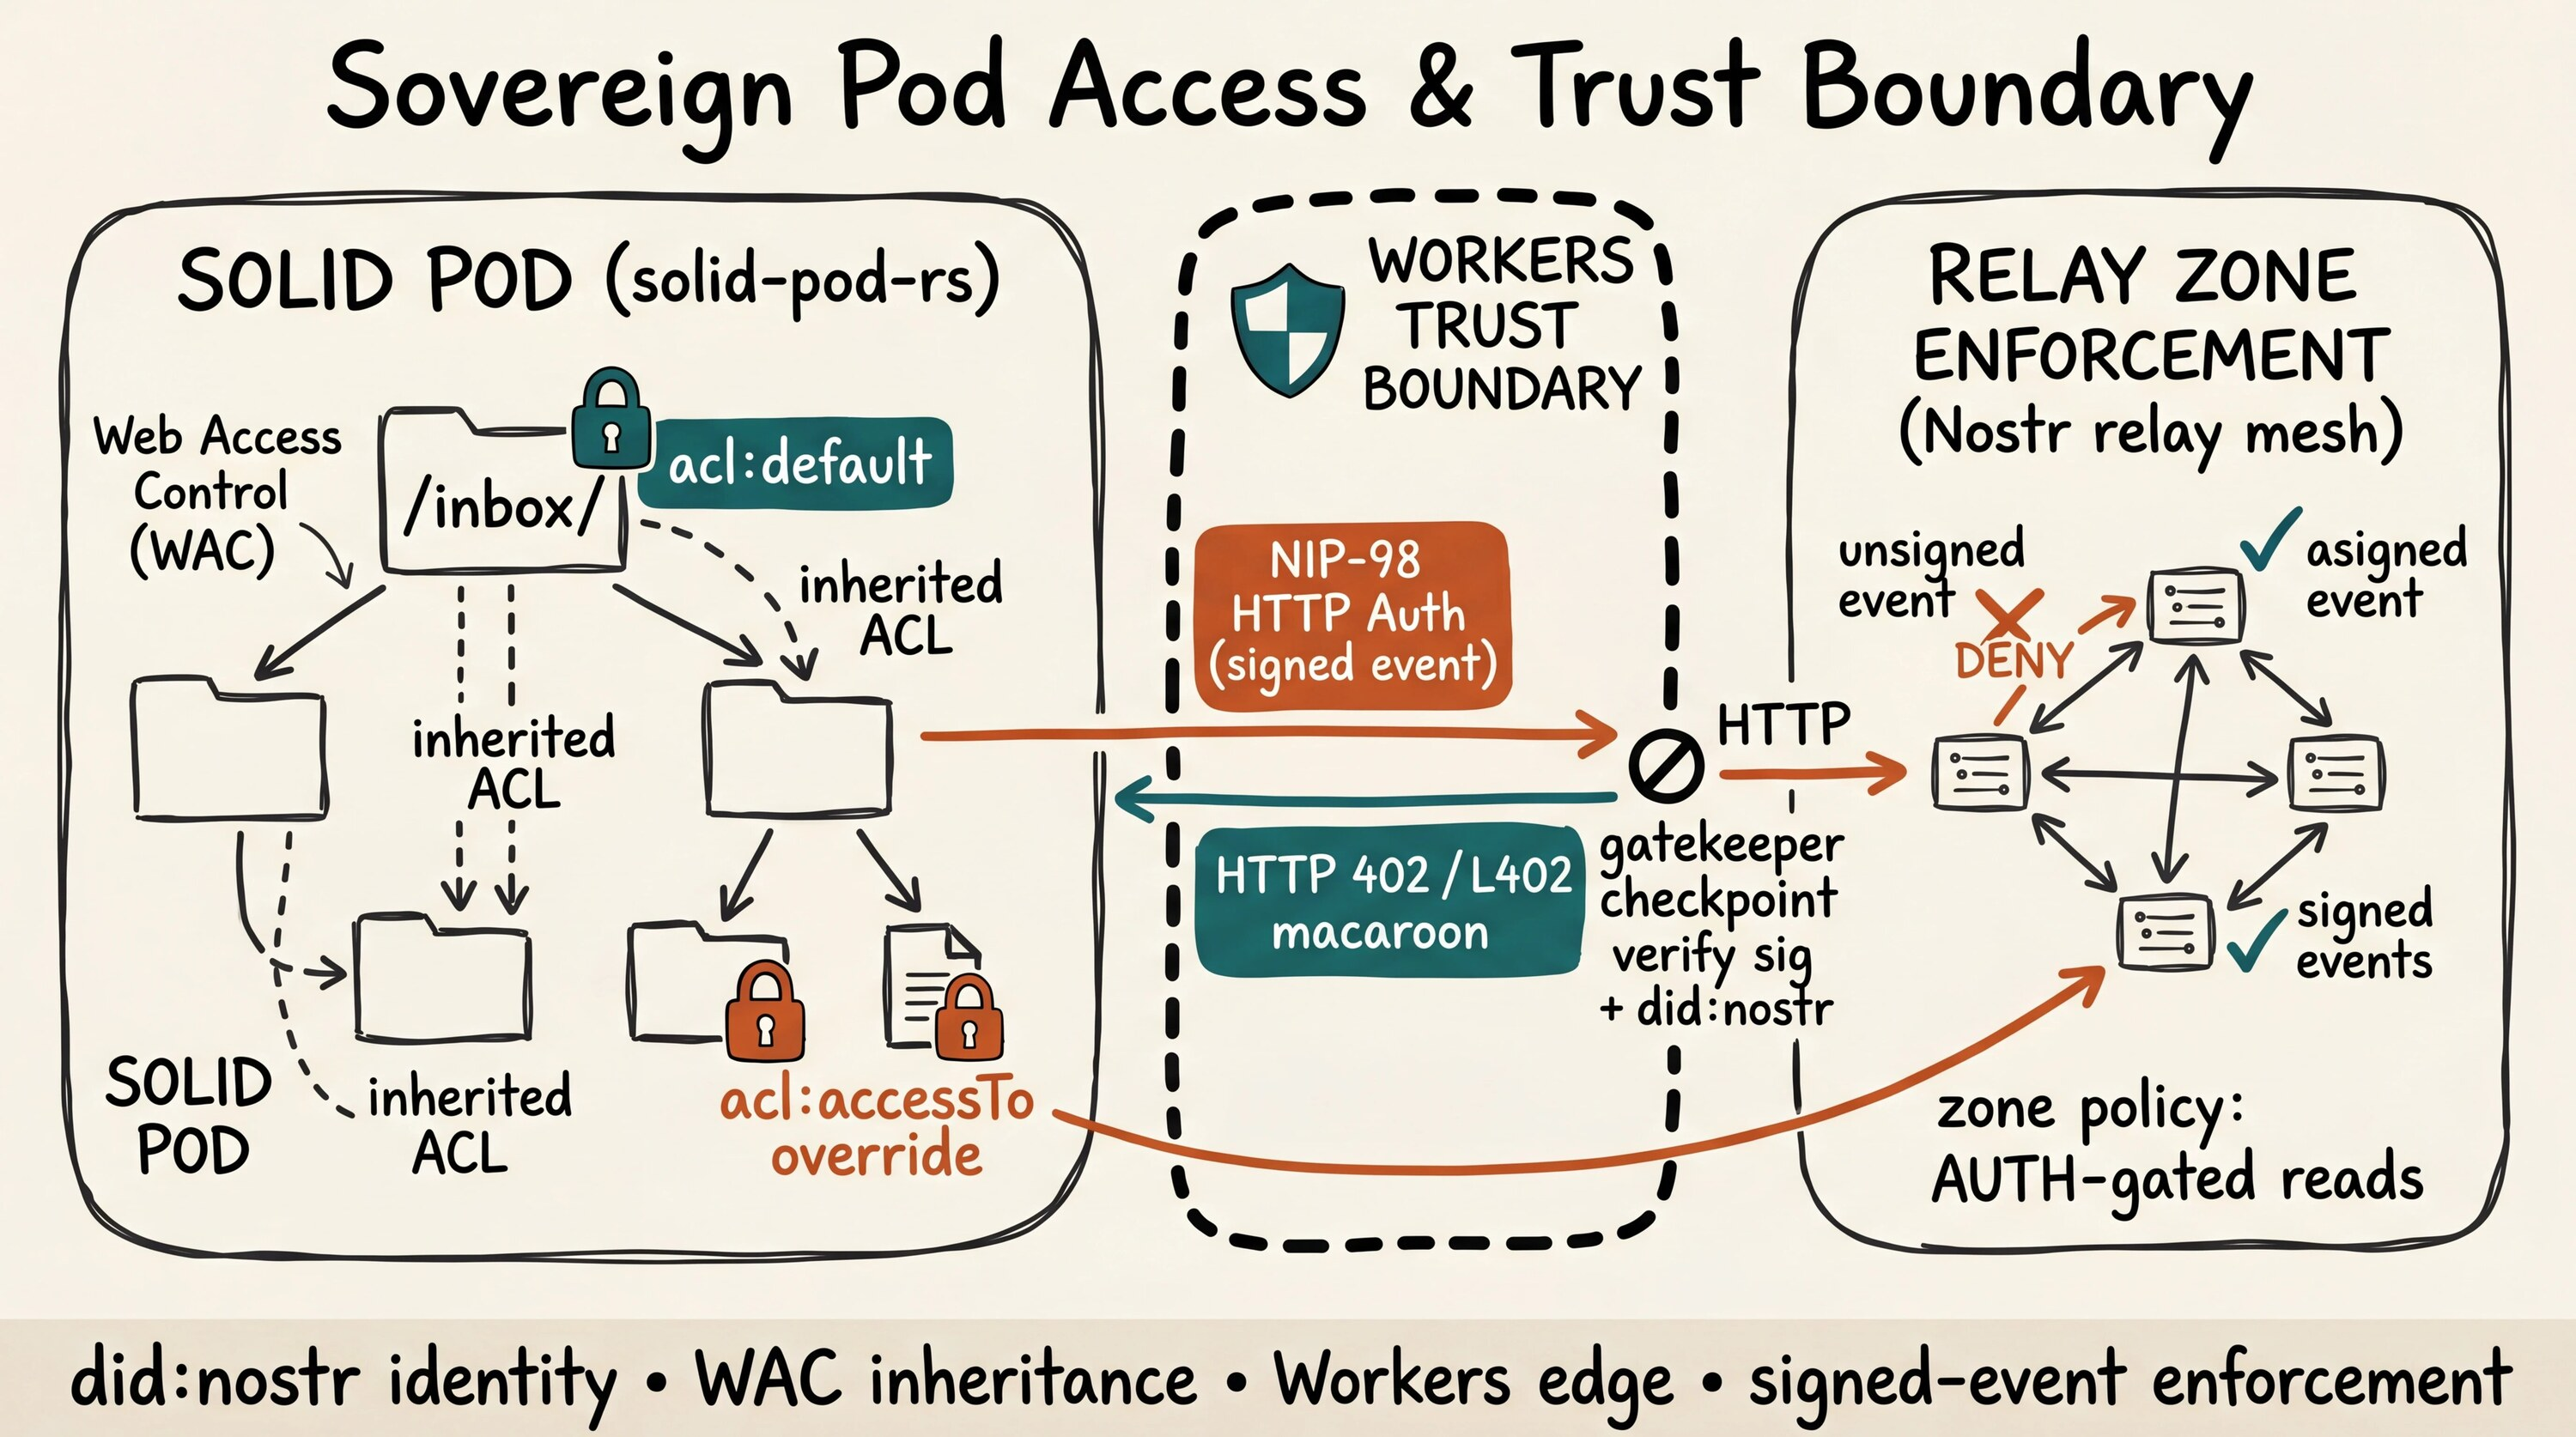
\includegraphics[width=0.9\textwidth]{hero-pod-boundary.jpg}
\caption{The pod trust boundary: WAC access control around actor-owned storage, with zoned access gated by \texttt{did:nostr} credentials. Illustration in the house sketch style.}
\label{fig:pod-boundary}
\end{figure}

\section{What a Pod Is}

\begin{definitionbox}[title={Pod}]
A personal data server the actor owns or chooses, storing data as RDF and gating every resource with a Web Access Control (WAC) list keyed to the actor's identity. Applications ask the pod for permission to read or write; the actor decides who gets access to what. Because the data format and the access rules are standardised, the actor can change applications without migrating data.
\end{definitionbox}

Solid (Social Linked Data) is a W3C specification, incubated by Tim Berners-Lee at MIT and now carried by the W3C Solid Community Group, whose reference implementation is JavaScriptSolidServer (JSS). solid-pod-rs is that reference implementation rewritten in Rust: a Cargo workspace of seven crates reporting roughly 96~per~cent strict parity with JSS on its own 207-row conformance tracker. The core crate carries the protocol primitives; sibling crates add identity, federation, and transport features (Table~\ref{tab:solid-crates}). The output is a single static binary with no Node.js dependency, deterministic RDF serialisation, and compile-time feature gating. Figure~\ref{fig:solidpod-arch} shows the three-layer architecture as rendered from the repository's own diagram-as-code sources.

\begin{figure}[h]
\centering
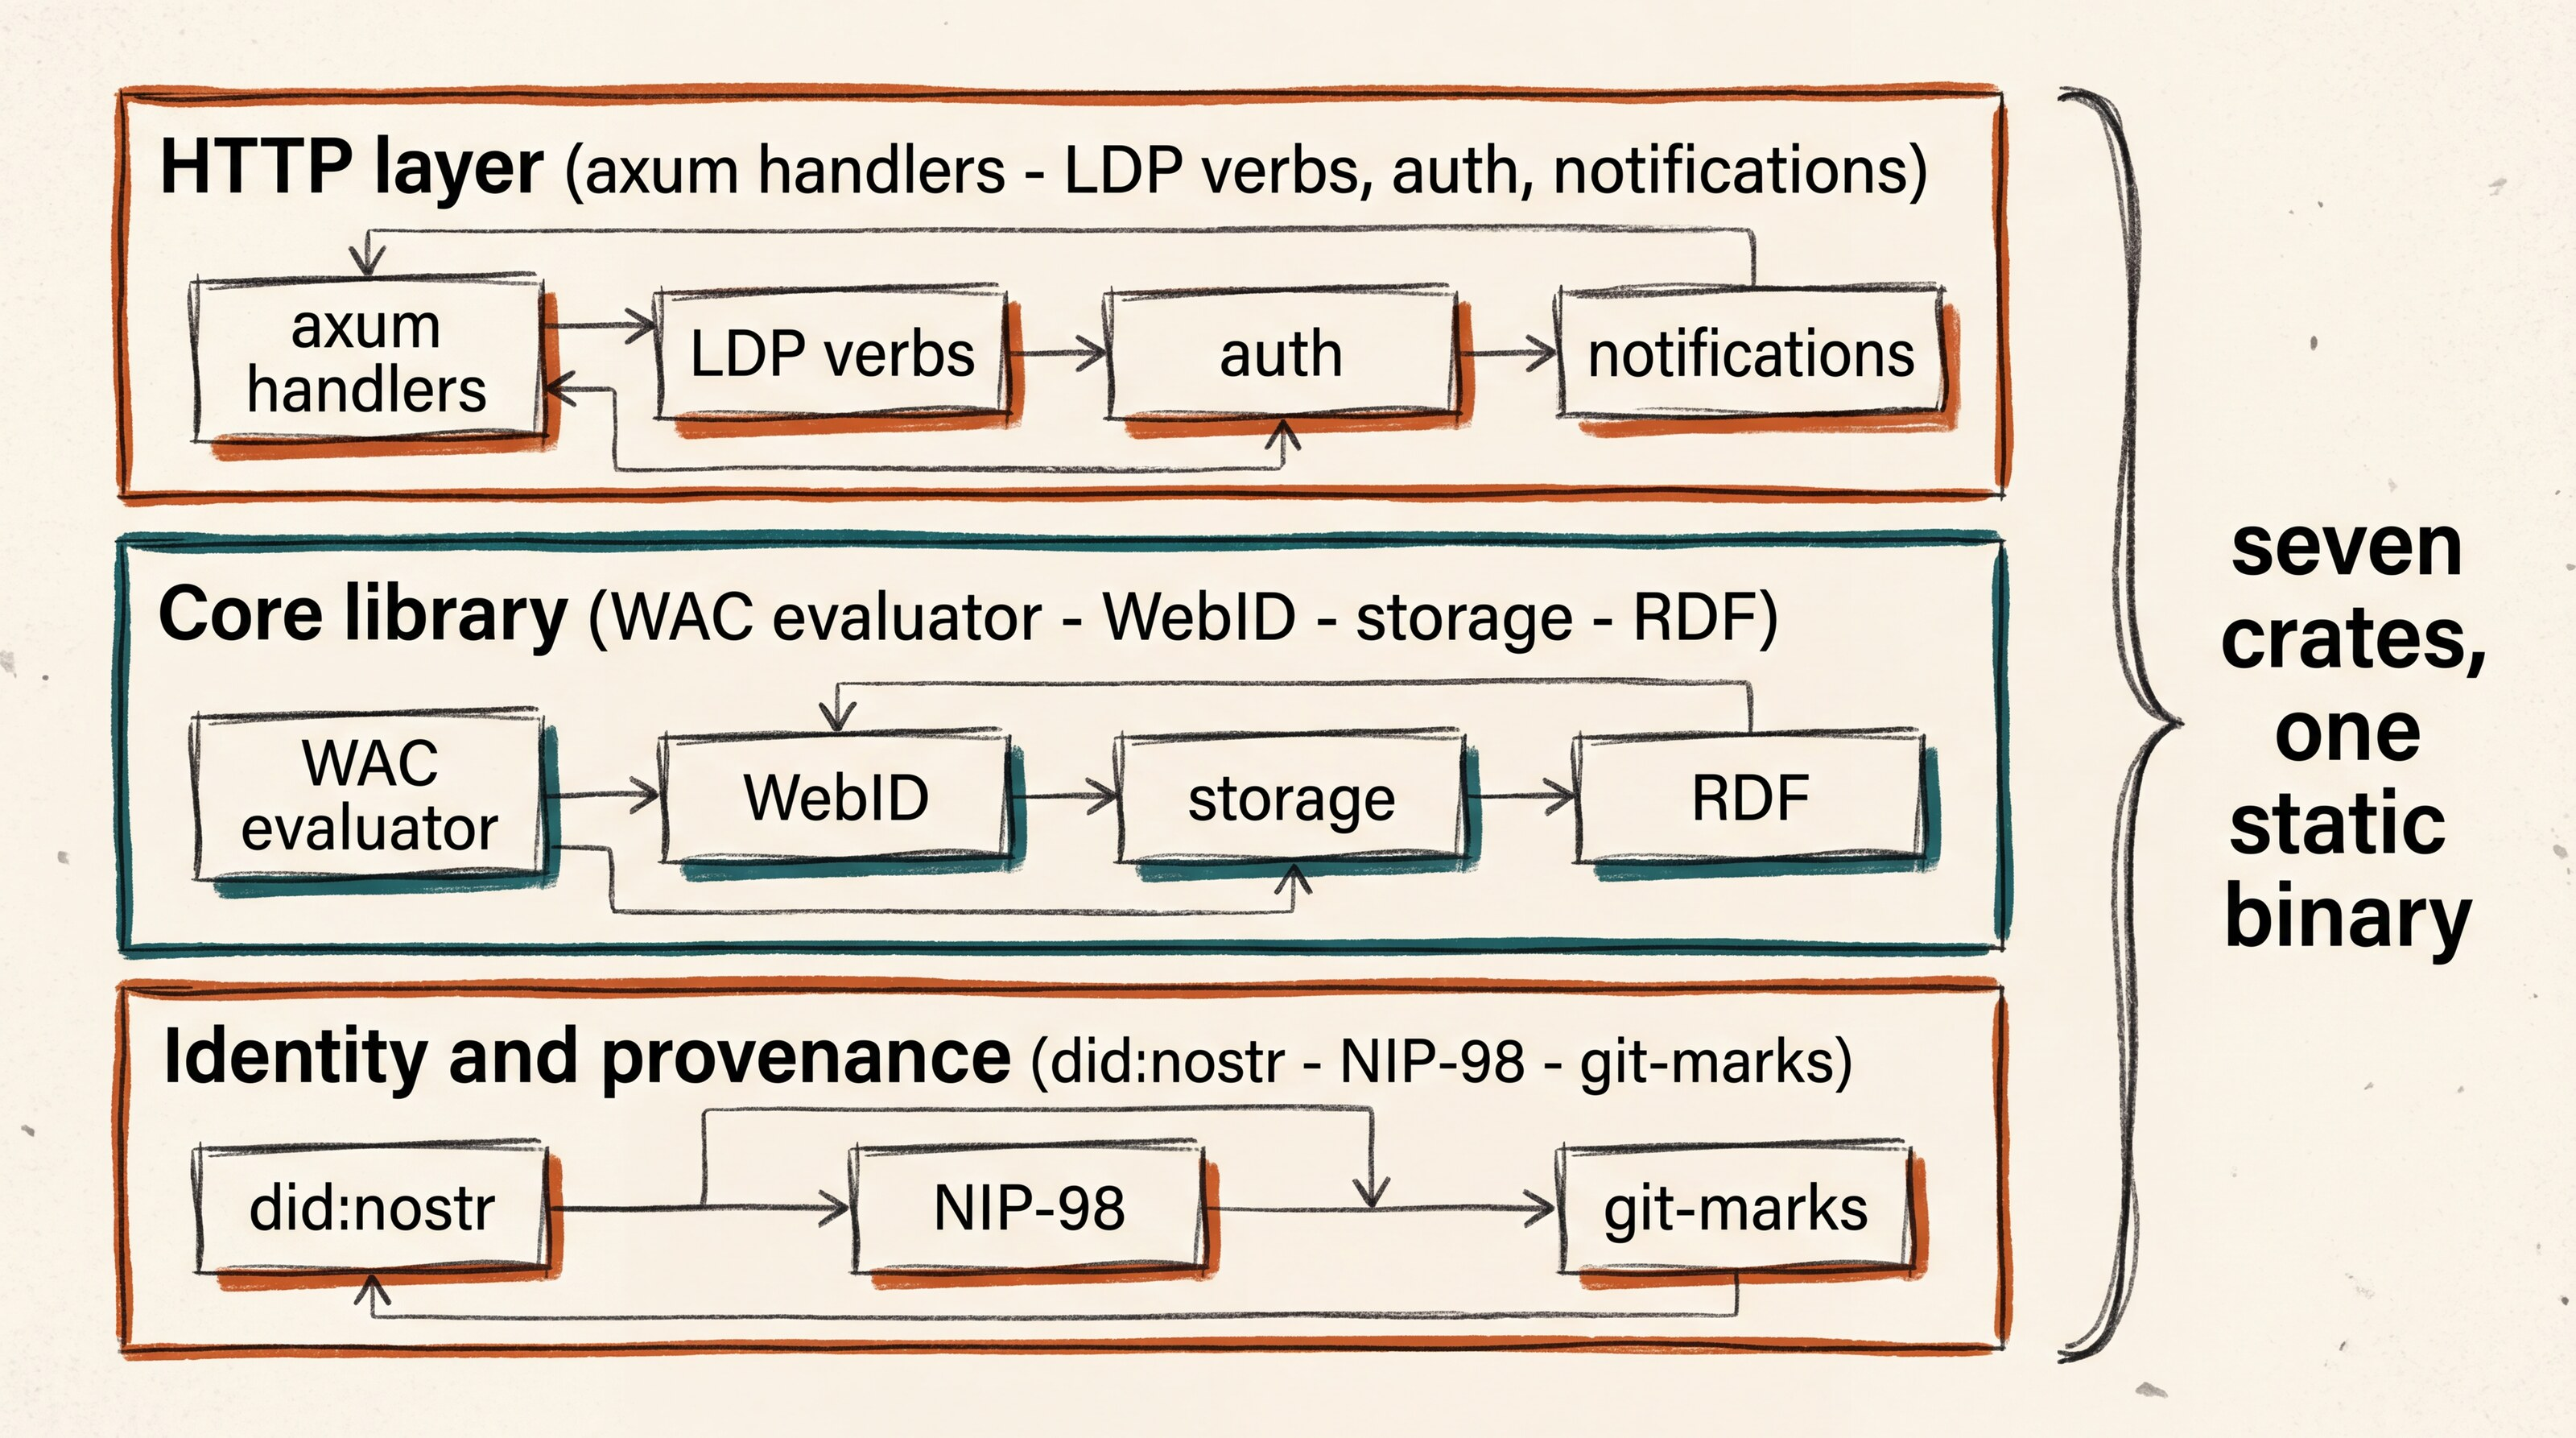
\includegraphics[width=0.95\textwidth]{nb-solidpod-arch.jpg}
\caption{solid-pod-rs in three bands: the axum HTTP layer, the core library, and the identity-and-provenance substrate --- seven crates, one static binary. Redrawn in the house style from the repository's architecture sources.}
\label{fig:solidpod-arch}
\end{figure}

\begin{table}[h]
\centering
\caption{The seven-crate workspace}
\label{tab:solid-crates}
\begin{tabularx}{\textwidth}{L{4.6cm} X}
\toprule
\textbf{Crate} & \textbf{Role} \\
\midrule
\texttt{solid-pod-rs} & Core library: LDP verbs, WAC evaluator, WebID, auth, notifications, storage \\
\addlinespace
\texttt{solid-pod-rs-server} & Drop-in server binary (actix-web + CLI) \\
\addlinespace
\texttt{solid-pod-rs-idp} & Solid-OIDC identity provider \\
\addlinespace
\texttt{solid-pod-rs-activitypub} & ActivityPub federation with HTTP Signatures \\
\addlinespace
\texttt{solid-pod-rs-nostr} & \texttt{did:nostr} resolver and NIP-01 relay \\
\addlinespace
\texttt{solid-pod-rs-git} & Git smart-HTTP backend behind WAC gates \\
\addlinespace
\texttt{solid-pod-rs-didkey} & \texttt{did:key} plus self-signed JWT verifier \\
\bottomrule
\end{tabularx}
\end{table}

Every pod speaks the Linked Data Platform. Each URL is a resource or a container, addressed with plain HTTP verbs: \texttt{GET} to read, \texttt{PUT} to create or replace, \texttt{POST} to add to a container, \texttt{PATCH} to edit in place, \texttt{DELETE} to remove. Access to each is decided by a WAC list that denies by default: no ACL means no access, and a policy set once at a container cascades to its descendants through \texttt{acl:default}. The modes are \texttt{acl:Read}, \texttt{acl:Write}, \texttt{acl:Append}, and \texttt{acl:Control}, and the principal a list names is a WebID or a \texttt{did:nostr}, evaluated against the same key the requester signed with.

In the governed maturity vocabulary of \texttt{ADR-002}, solid-pod-rs sits between \texttt{standalone} and \texttt{integrated}. It runs as a standalone pod server today; its wiring into the wider mesh, reachable over the same three federation transports as every other component (a private Tailscale tailnet, the Nostr relay strata, and Cloudflare tunnels), is real but incomplete for reasons the closeout audit made precise and this chapter states plainly below.

It is pre-1.0 software, still hardening, and licensed AGPL-3.0. Operating a pod as a network service, which by the nature of a pod an operator almost always will, obliges that operator to provide corresponding source to its users. Copyleft is here a sovereignty mechanism, not a licensing footnote.

\section{One Keypair, Every Boundary}

The identity model is the reason a pod in this ecosystem amounts to more than storage. One secp256k1 keypair, the actor's \texttt{did:nostr}, is at once the relay identity, the HTTP authentication identity, the WAC principal that access-control lists name, the author recorded in every provenance record, and the subject of the DID document. There are no session stores, no token-exchange dance, no per-service credential to provision or rotate. An agent that authenticates to a pod with a NIP-98 request signature (a per-request Nostr event, kind 27235, binding URL, method, and body hash) is authenticated as exactly the principal that a WAC list grants or denies, and as exactly the principal a provenance record will attribute the write to.

This collapses a class of trust problem that federated systems usually solve with brokered credentials. When the WAC evaluator asks who is making a request, the answer is a public key that verified a Schnorr signature moments earlier, not a bearer token minted by an intermediary both parties must trust.

The 2026-07-03 closeout release made that path fail-closed. BIP-340 signature verification, which previously ran only under an optional feature and would silently degrade to structural checks without it, is now unconditional; a build that drops the verification code fails to compile rather than accepting forged public keys. The same release added a single-use replay guard so a captured authentication header cannot be re-presented inside its timestamp window, and wired \texttt{acl:origin} enforcement into the request path so cross-origin ACL restrictions stop being inert. Four security issues were closed in that one release, and the identity spine they protect is the whole point of the component. The gap-close sprint then lifted that replay guard's backing store into a \texttt{ReplayStore} trait in the core crate, its single documented edge exception recorded rather than hidden (\texttt{40043b0}), so the guard is now a pluggable seam rather than a fixed in-memory cache.

\section{Every Write a Commit}

A pod records who changed what, when, and on whose authority. solid-pod-rs makes that record first-class through two composable provenance primitives, cost-tiered so the cheap one is always on.

\emph{git-marks} run on every LDP write. Each \texttt{PUT}, \texttt{POST}, and \texttt{PATCH} becomes a git commit, captured and persisted as a PROV-O sidecar at \texttt{<resource>.prov.ttl}. The result is content-addressed, append-only, tamper-evident ordering of every write and a queryable history of who wrote each resource, for free, on every pod. The \texttt{PATCH} case earns a specific receipt, because an in-place edit is where a naive implementation silently clobbers unrelated triples: \texttt{seed\_graph\_from\_patch\_target} makes the edit non-destructive, and a three-case regression suite pins that property in place (\texttt{791977a}), so the commit a \texttt{PATCH} records is a true delta rather than a rewrite.

\emph{block-trails} are the opt-in high-value tier: a Bitcoin-taproot-anchored, hash-chained state trail that irreversibly timestamps a record against the Bitcoin chain, so no single party, not even the pod operator, can forge or silently rewrite it. To keep on-chain cost amortised, an epoch Merkle root over a batch of commits is anchored in a single transaction, and anchoring is reserved for records whose ACL flags them anchor-worthy.

This is the concrete substrate behind the canon's claim that ``the graph is the audit trail'' (Chapter~\ref{ch:visionflow-canon}). Provenance here is a structural guarantee of the write path rather than a log the write path emits alongside its real work and might forget to. Every change is attributable to a commit; every high-value change carries an external proof anyone can check without trusting the pod. That property is what lets an escalated agent action reach a human judgment broker (Chapter~\ref{ch:role-transformation}) with its evidence and its authorship intact, and what makes the ecosystem's data moat a moat of \emph{trace}, who proposed what on what evidence and what a human decided, rather than of raw data alone. The gap-close sprint gave that trace a defined shape to read back: a \texttt{\_prov/} enumeration contract now specifies how a caller walks a resource's provenance sidecars as a set (\texttt{40043b0}), with the serving endpoint specified and scheduled rather than yet bound.

Value transmission is further along than the umbrella canon's ``402 web-ledger'' metering framing (Chapter~\ref{ch:visionflow-canon}) admits: solid-pod-rs ships a working peer-to-peer exchange (an order book, a constant-product automated-market-maker pool, and a from-scratch BIP-341 taproot transaction builder) behind route-tested \texttt{/pay/.swap} and \texttt{/pay/.pool} endpoints, leaving only live mainnet settlement unproven.

\section{Acting Under a Mandate}

The hardest question a shared data layer has to answer is how an agent writes to a human's pod without becoming the human. The canon's answer is the mandate model, and it is a good answer. An agent acts as itself, under a scoped WAC \texttt{acl:agent} grant named \texttt{urn:agentbox:mandate}, and never by holding the human's \texttt{nsec}. The agent's own \texttt{did:nostr} appears in the human's pod ACL with specific modes on specific resources; the agent authenticates with its own key; and every write it makes is attributed, in the provenance trail, to the agent and not to the human who delegated to it.

The espoused model and the shipped mechanism diverge on one axis, and the 2026-07-03 closeout names the divergence rather than papering over it. A mandate has three properties that distinguish it from a handed-over key. Two hold today; one does not (Table~\ref{tab:mandate-properties}).

\begin{table}[h]
\centering
\caption{The mandate model, espoused versus shipped}
\label{tab:mandate-properties}
\begin{tabularx}{\textwidth}{L{3.2cm} X L{2.4cm}}
\toprule
\textbf{Property} & \textbf{What it requires} & \textbf{Shipped?} \\
\midrule
Attribution & Agent authenticates and is provenance-logged as its own \texttt{did:nostr}, never the human's & Yes \\
\addlinespace
Least authority & Grant is scoped to declared \texttt{acl:mode} on declared resources & Yes \\
\addlinespace
Revocability & Expiry field the WAC evaluator enforces; a revocation event; a reconciler that propagates withdrawal & No \\
\bottomrule
\end{tabularx}
\end{table}

Revocability is asserted in prose but not enforced in code. The mandate is currently a static, non-expiring ACL grant: the WAC evaluator reads it and honours it, but there is no expiry field it checks, no replaceable-event revocation semantics it observes, and no reconciler that would propagate a withdrawal to the pod's access-control state. The canon names the primitive without specifying how revocation reaches the evaluator that would have to act on it.

\begin{cautionbox}[title={Delegation versus impersonation}]
A mandate with no revocation clock is a standing grant. It is materially better than key-sharing on two of three axes, since the agent is attributable as itself and its authority is scoped, so it is not impersonation. A delegation the human cannot withdraw is, even so, not yet the revocable mandate the canon promises. The gap is named here, at the point of the claim, because revocation is the exact property that separates lending authority from surrendering it. Closing it needs an expiry field the evaluator enforces, a replaceable-event revocation path, and a reconciler cadence; none of the three is wired today. Chapter~\ref{ch:gap-register} carries this in the systematic register; this chapter's job is only to refuse to let the espoused version stand in for the shipped one.
\end{cautionbox}

\section{A Rich Library Behind a Thin Server}

The independent closeout deep-dive of 2026-07-03 (ten comparison dimensions, each analysed and then adversarially re-verified against JSS as baseline) returned a verdict worth quoting in shape.

\begin{evidencebox}[title={Library present is not server wired}]
solid-pod-rs is a high-quality library port behind a thin reference server. The crate-level modules are, in several places, richer and more hardened than the JSS original: a single-use replay cache, argon2 password hashing, SSRF classification, durable federation delivery with backoff, an ACL-lockout guard the reference lacks, and correct deny-by-default access control. The shipped \texttt{solid-pod-rs-server} binds only a slice of what the libraries implement, and the parity checklist measures library \emph{presence}, not deployed HTTP \emph{behaviour}, so the headline parity figure overstates what a running pod actually serves.
\end{evidencebox}

The examples are specific:

\begin{itemize}
  \item The ActivityPub crate is a workspace member but not a dependency of the server binary, so federation is fully built, unit-tested, and unreachable over HTTP.
  \item The Solid-OIDC provider implements discovery, JWKS, and the full authorisation-code flow but exposes an axum router the actix server never mounts, so OIDC discovery is broken end to end while the checklist marks the rows present.
  \item \texttt{acl:agentGroup} is the sharpest case. The library implements group-based access control, but the server passes an empty resolver at every call-site, so at runtime it is a no-op identical to the reference implementation's stub.
\end{itemize}

The audit's discipline is the one this whole report argues for. For each unwired surface the choice is binary: finish the wiring, or relabel the row honestly as \emph{library-only, not server-wired}. What is not acceptable is a checklist claiming ``present'' for a capability a deployed pod cannot serve.

That posture is why solid-pod-rs earns a chapter in Part~\ref{part:visionflow} rather than a line in a product sheet. The cryptographic foundation is real, the provenance is real, the identity model is the right one, and the four security fixes landed. The gaps, an unenforced mandate and a server that binds a subset of its own library, are named at the point of the claim, in print, before the next edition can quietly close or quietly forget them. Data that belongs to its actor is the correct design. Making the deployed server enforce all of what the library already knows how to do is the work between the design and the promise.

\chapter{Shared Semantics on a Budget: The Ontology Binding}
\label{ch:ontology-binding}

\epigraph{A shared vocabulary is only shared if every agent can afford to read it.}{}

\section{What the Binding Is}

Every other chapter in this part describes infrastructure that one agent owns. This
chapter describes the one piece all of them share: a formal ontology, and a mechanism for
reaching it that reaches every agent turn without asking any agent to carry the whole
graph in its head. The mechanism is the pervasive ontology binding, specified in
\texttt{PRD-020} and its keystone decision record \texttt{ADR-112}.

The corpus is a formal OWL~2 ontology held in VisionClaw's Oxigraph store (RocksDB-backed
RDF, materialised inference), with Whelk EL++ as the reasoner. The live semantic index
carried 5,975 class summaries when captured for the skill documentation on 14 June 2026.
That headline needs a caveat the book's ethic demands: the authored terminology is roughly
4,952 \texttt{owl:Class} definitions plus about 9,766 label-only stubs, and the retrieval
index is sized for around 14,718 entries once stubs are counted. Three numbers describe one
corpus at different levels of authoring, and the honest citation is \emph{roughly six
thousand authored classes over a moving base}; Chapter~\ref{ch:gap-register} holds the
reconciliation this ecosystem cannot reliably perform on itself.

That corpus has a lineage worth stating plainly. It is extracted, through a
Logseq-to-OWL tool, from the operator's own multi-year research notebook rather than
from a scraped or third-party dataset, which is why it carries classes for the operator's
former laboratories, \texttt{nicve-virtual-reality-research-centre} and
\texttt{octave-immersive-research-facility}, beside a numbered telepresence taxonomy of
co-presence, mutual gaze, proxemics, and common-ground theory. That taxonomy is a formal
encoding of the same literature this report's 2022 predecessor \parencite{OHare2022Convergence}
drew on for its telepresence chapter. The honest limit of the claim is that no class in the
local snapshot cites that book by name or DOI: a search for the title and its arXiv
identifier returned nothing, and the live graph was unreachable during this reconciliation
pass (see the fail-open section below), so the evidence rests on the static snapshot rather
than a live traversal. The defensible reading is shared authorial descent from one
continuing research programme, where the ontology is the later and much larger encoding of
notes that also fed the book, a corpus since grown well past book-era scope into robotics,
supply-chain, and security domains the book never covered.

The binding's central design choice is a refusal to add a service. A sixteen-agent design
pass first proposed a fresh HTTP route (an ``ontology ask'' endpoint inside the management
API), and adversarial review took that form apart: the management API is Fastify, so the
proposed Express router would not have mounted; it would have forced a second secret domain
onto every isolated consultant subprocess; and a per-turn network round-trip is heavier
than the sub-fifteen-millisecond local lookup the injection hook already budgets for. The
corrected design makes the retrieval logic a shared in-process library
(\texttt{agentbox/mcp/servers/lib/ontology-retrieval.js}) that each caller constructs its
own copy of. One module and two shared backing stores, with no extra authentication wall
between an agent and the graph.

\begin{figure}[h]
\centering
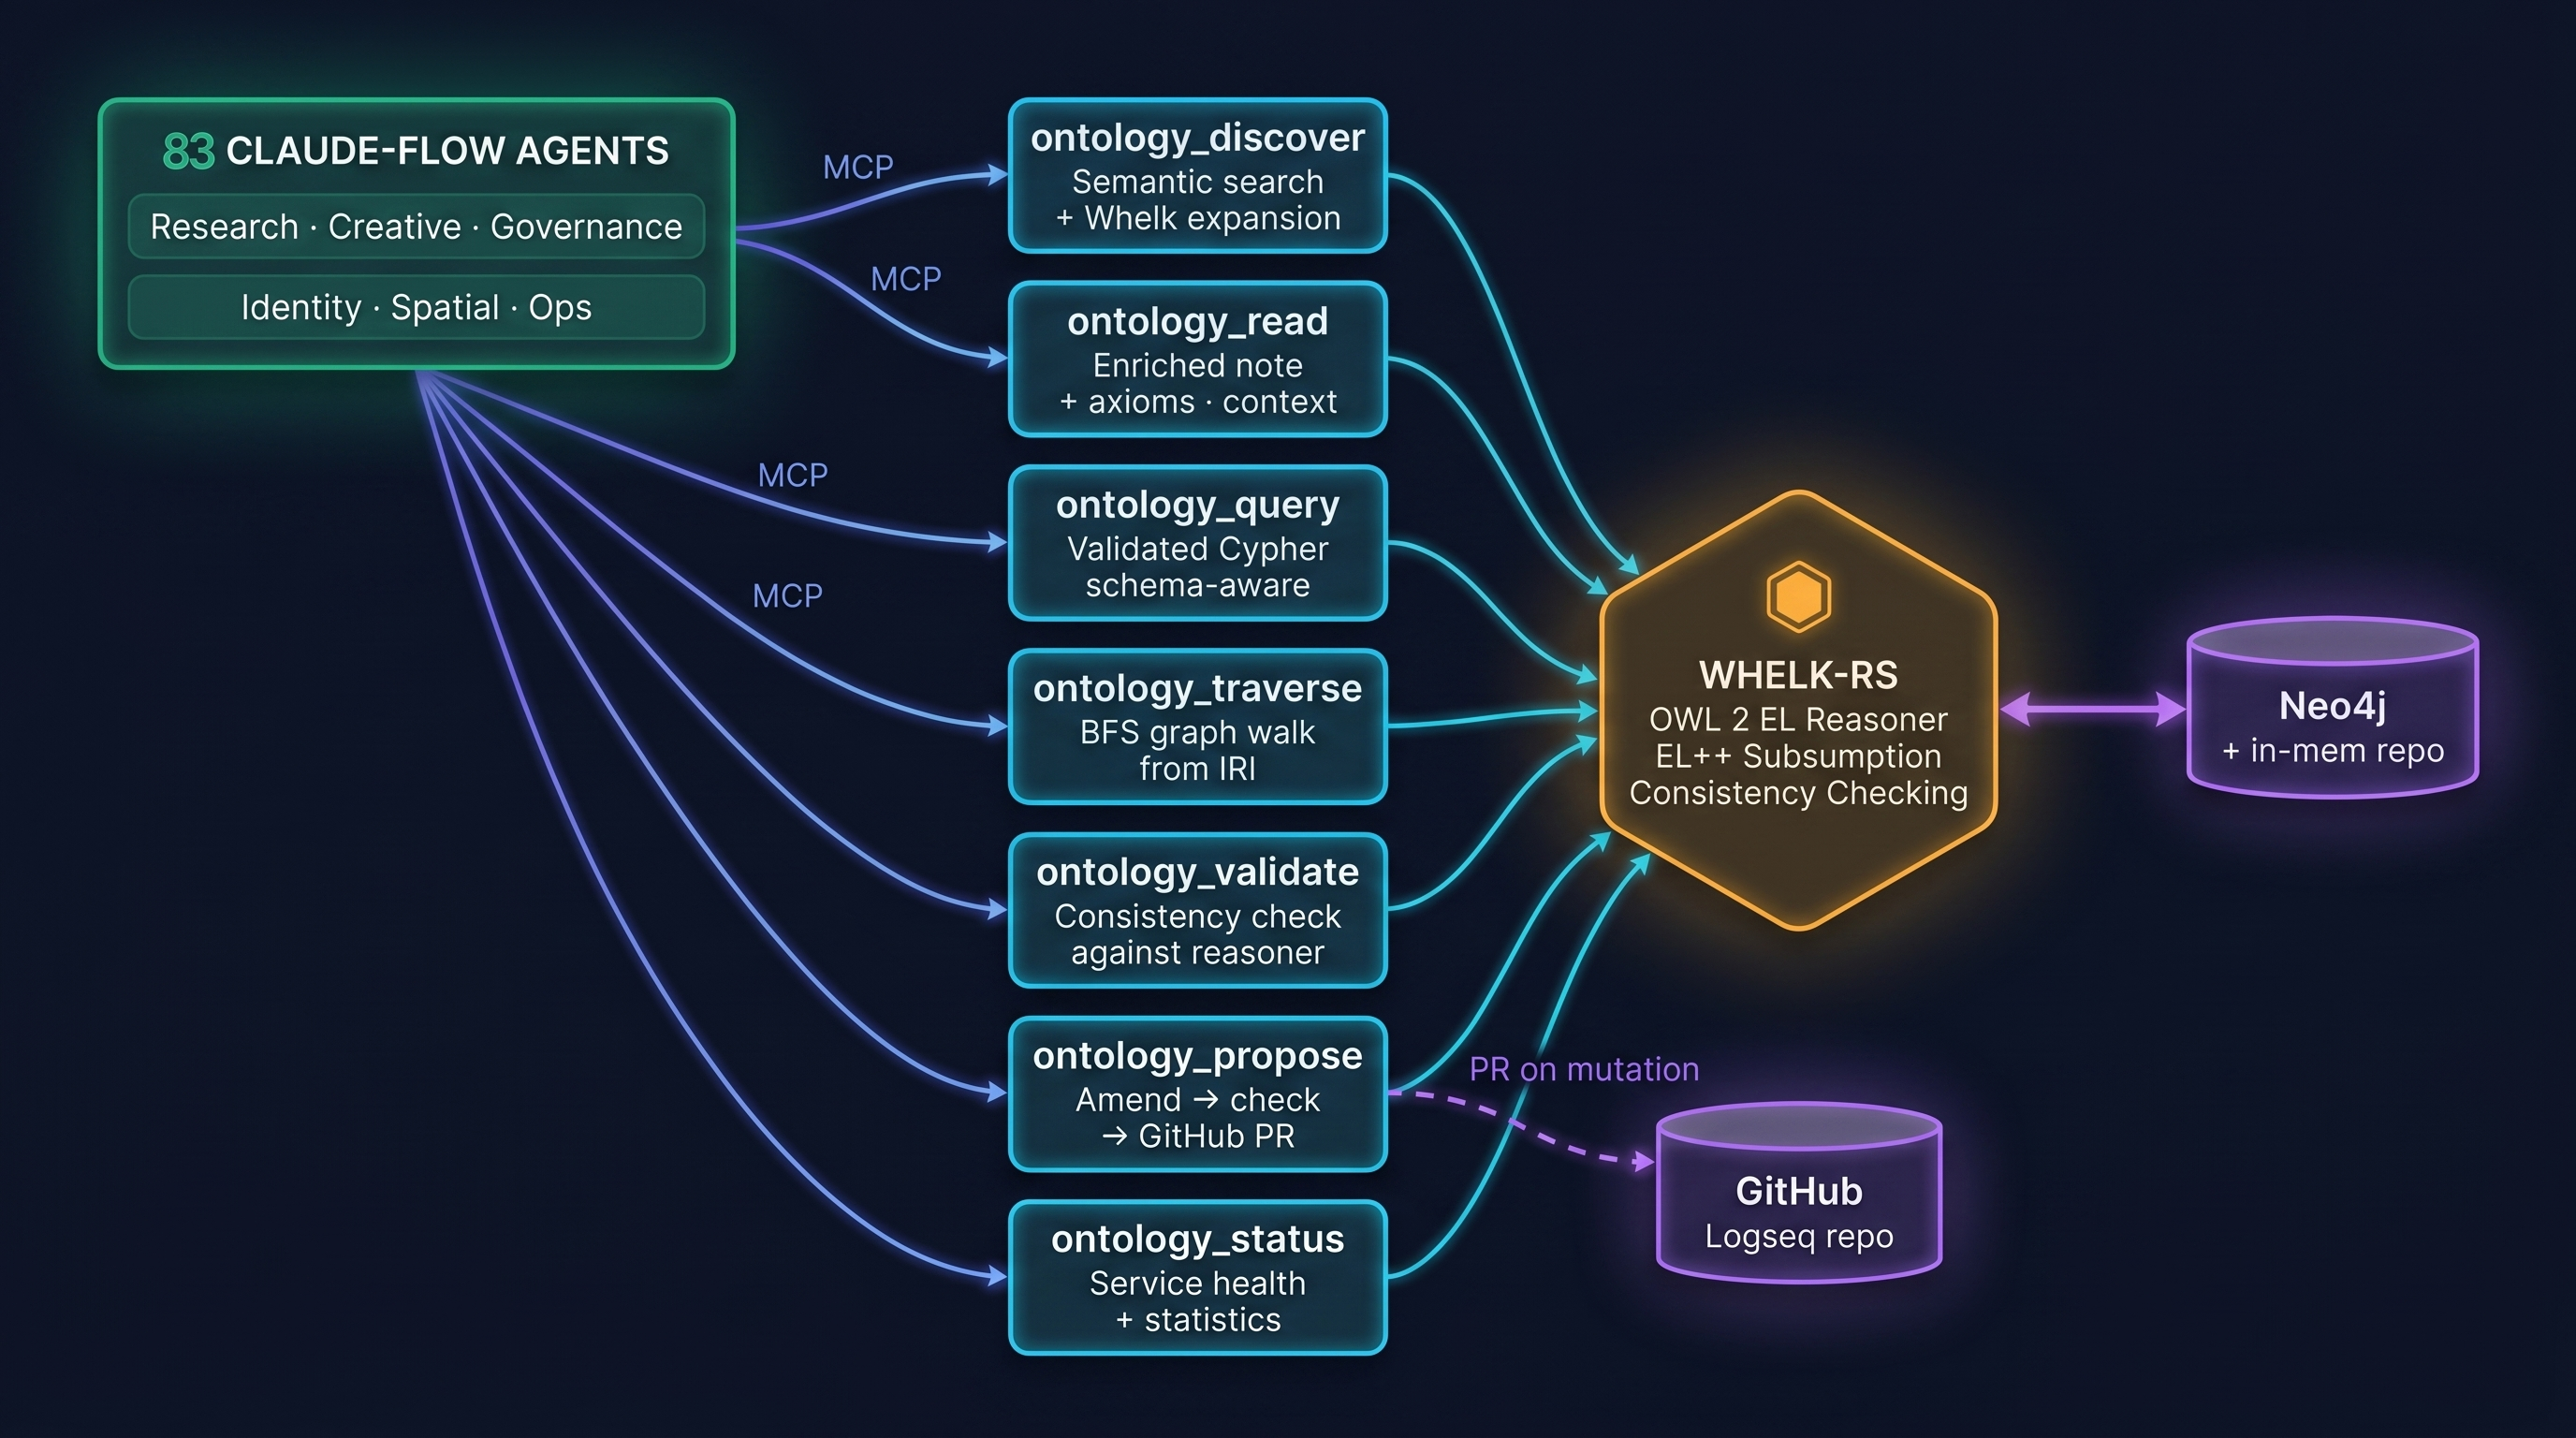
\includegraphics[width=0.88\textwidth]{diag-mcp-radial.png}
\caption{The ontology tool surface: MCP tools arranged around the Oxigraph store and Whelk EL++ reasoner. Rendered from the ecosystem's diagram-as-code corpus.}
\label{fig:ontology-tools}
\end{figure}

\section{Two Channels: Ambient Push, Deliberate Pull}

The binding reaches an agent through two channels with deliberately different economics.
\textbf{PUSH} is ambient. On every interactive turn, a synchronous hook
(\texttt{claude-flow-hook-adapter.cjs}) scores the prompt against a pre-warmed class
index using trigram Jaccard similarity and, only when the top score clears a relevance
floor (\texttt{ONTOLOGY\_PUSH\_MIN\_RELEVANCE}, default \texttt{0.11}), emits one line of
about 80 tokens naming the most relevant seed class with its maturity and domain. The
floor is the point of the channel. An on-topic prompt gets a breadcrumb; an off-topic one
gets silence. ``Remind me where we are up to please'' scores below the floor and produces
nothing, while ``design an escrow contract with an oracle'' surfaces the
\texttt{optimistic-oracle} class. No agent invokes PUSH; it appears, or it does not. It
never touches the network on the hot path: a breadcrumb waiting on an embedding round-trip
would blow the hook's latency budget and emit nothing at all.

\textbf{PULL} is deliberate. An agent that wants grounding calls \texttt{ontology\_ask}
and receives a provenance-scoped Turtle subgraph, budget-bounded by the calling model's
tier. The tier does the rationing: a cheaper model gets a tighter subgraph, an expensive
one gets depth and inferred closure, and the budget is enforced in the library after
serialisation rather than left to each caller's discretion (\texttt{ADR-116}).
Table~\ref{tab:ontology-tiers} states the ceilings.

\begin{table}[h]
\centering
\caption{Model-tier budgets for \texttt{ontology\_ask} (ADR-116)}
\label{tab:ontology-tiers}
\begin{tabularx}{\textwidth}{L{2.6cm} X L{2.4cm}}
\toprule
\textbf{Tier} & \textbf{Retrieval mode} & \textbf{Token ceiling} \\
\midrule
booster (PUSH) & breadcrumb; synchronous local trigram match; depth 0; asserted graph & $\leq$80 \\
\addlinespace
haiku & class-summary menu; depth 0; asserted graph & $\leq$500 \\
\addlinespace
sonnet & depth-1 neighbourhood in terse Turtle; asserted; full page bodies chunked to budget & $\leq$2{,}000 \\
\addlinespace
opus & depth-2 plus inferred closure, layer-labelled & $\leq$6{,}000 \\
\bottomrule
\end{tabularx}
\end{table}

One detail of the expand path looks trivial and is not. Because the asserted graph stores
only \texttt{child subClassOf parent}, a seed's subclasses are incoming edges that a purely
outgoing expansion missed; the query now fetches children first and places them ahead of
the budget clamp so they survive it (a measured gap, fixed 14 June). Terse Turtle over
SPARQL-results JSON buys a two-to-ninefold token reduction (\texttt{ADR-115}), most of why
a six-thousand-class corpus fits a two-thousand-token sonnet budget at all.

\begin{evidencebox}[title={A captured pull: matching by meaning}]
Asked for ``escrow oracle payment settlement'' at sonnet tier, \texttt{ontology\_ask}
returned a 146-token subgraph seeded on \texttt{price-oracle} and
\texttt{cbdc-cross-border-settlement}, classes whose labels share no literal term with the
query. The retrieval is embedding-seeded against the class index, so it finds the
contract domain by meaning rather than by string match. The same query at haiku tier
returns a tighter subgraph: the tier drives the budget, and the budget drives how much of
the graph the agent ever sees. (Live capture, \texttt{visionclaw-server}, 14 June 2026.)
\end{evidencebox}

\begin{figure}[h]
\centering
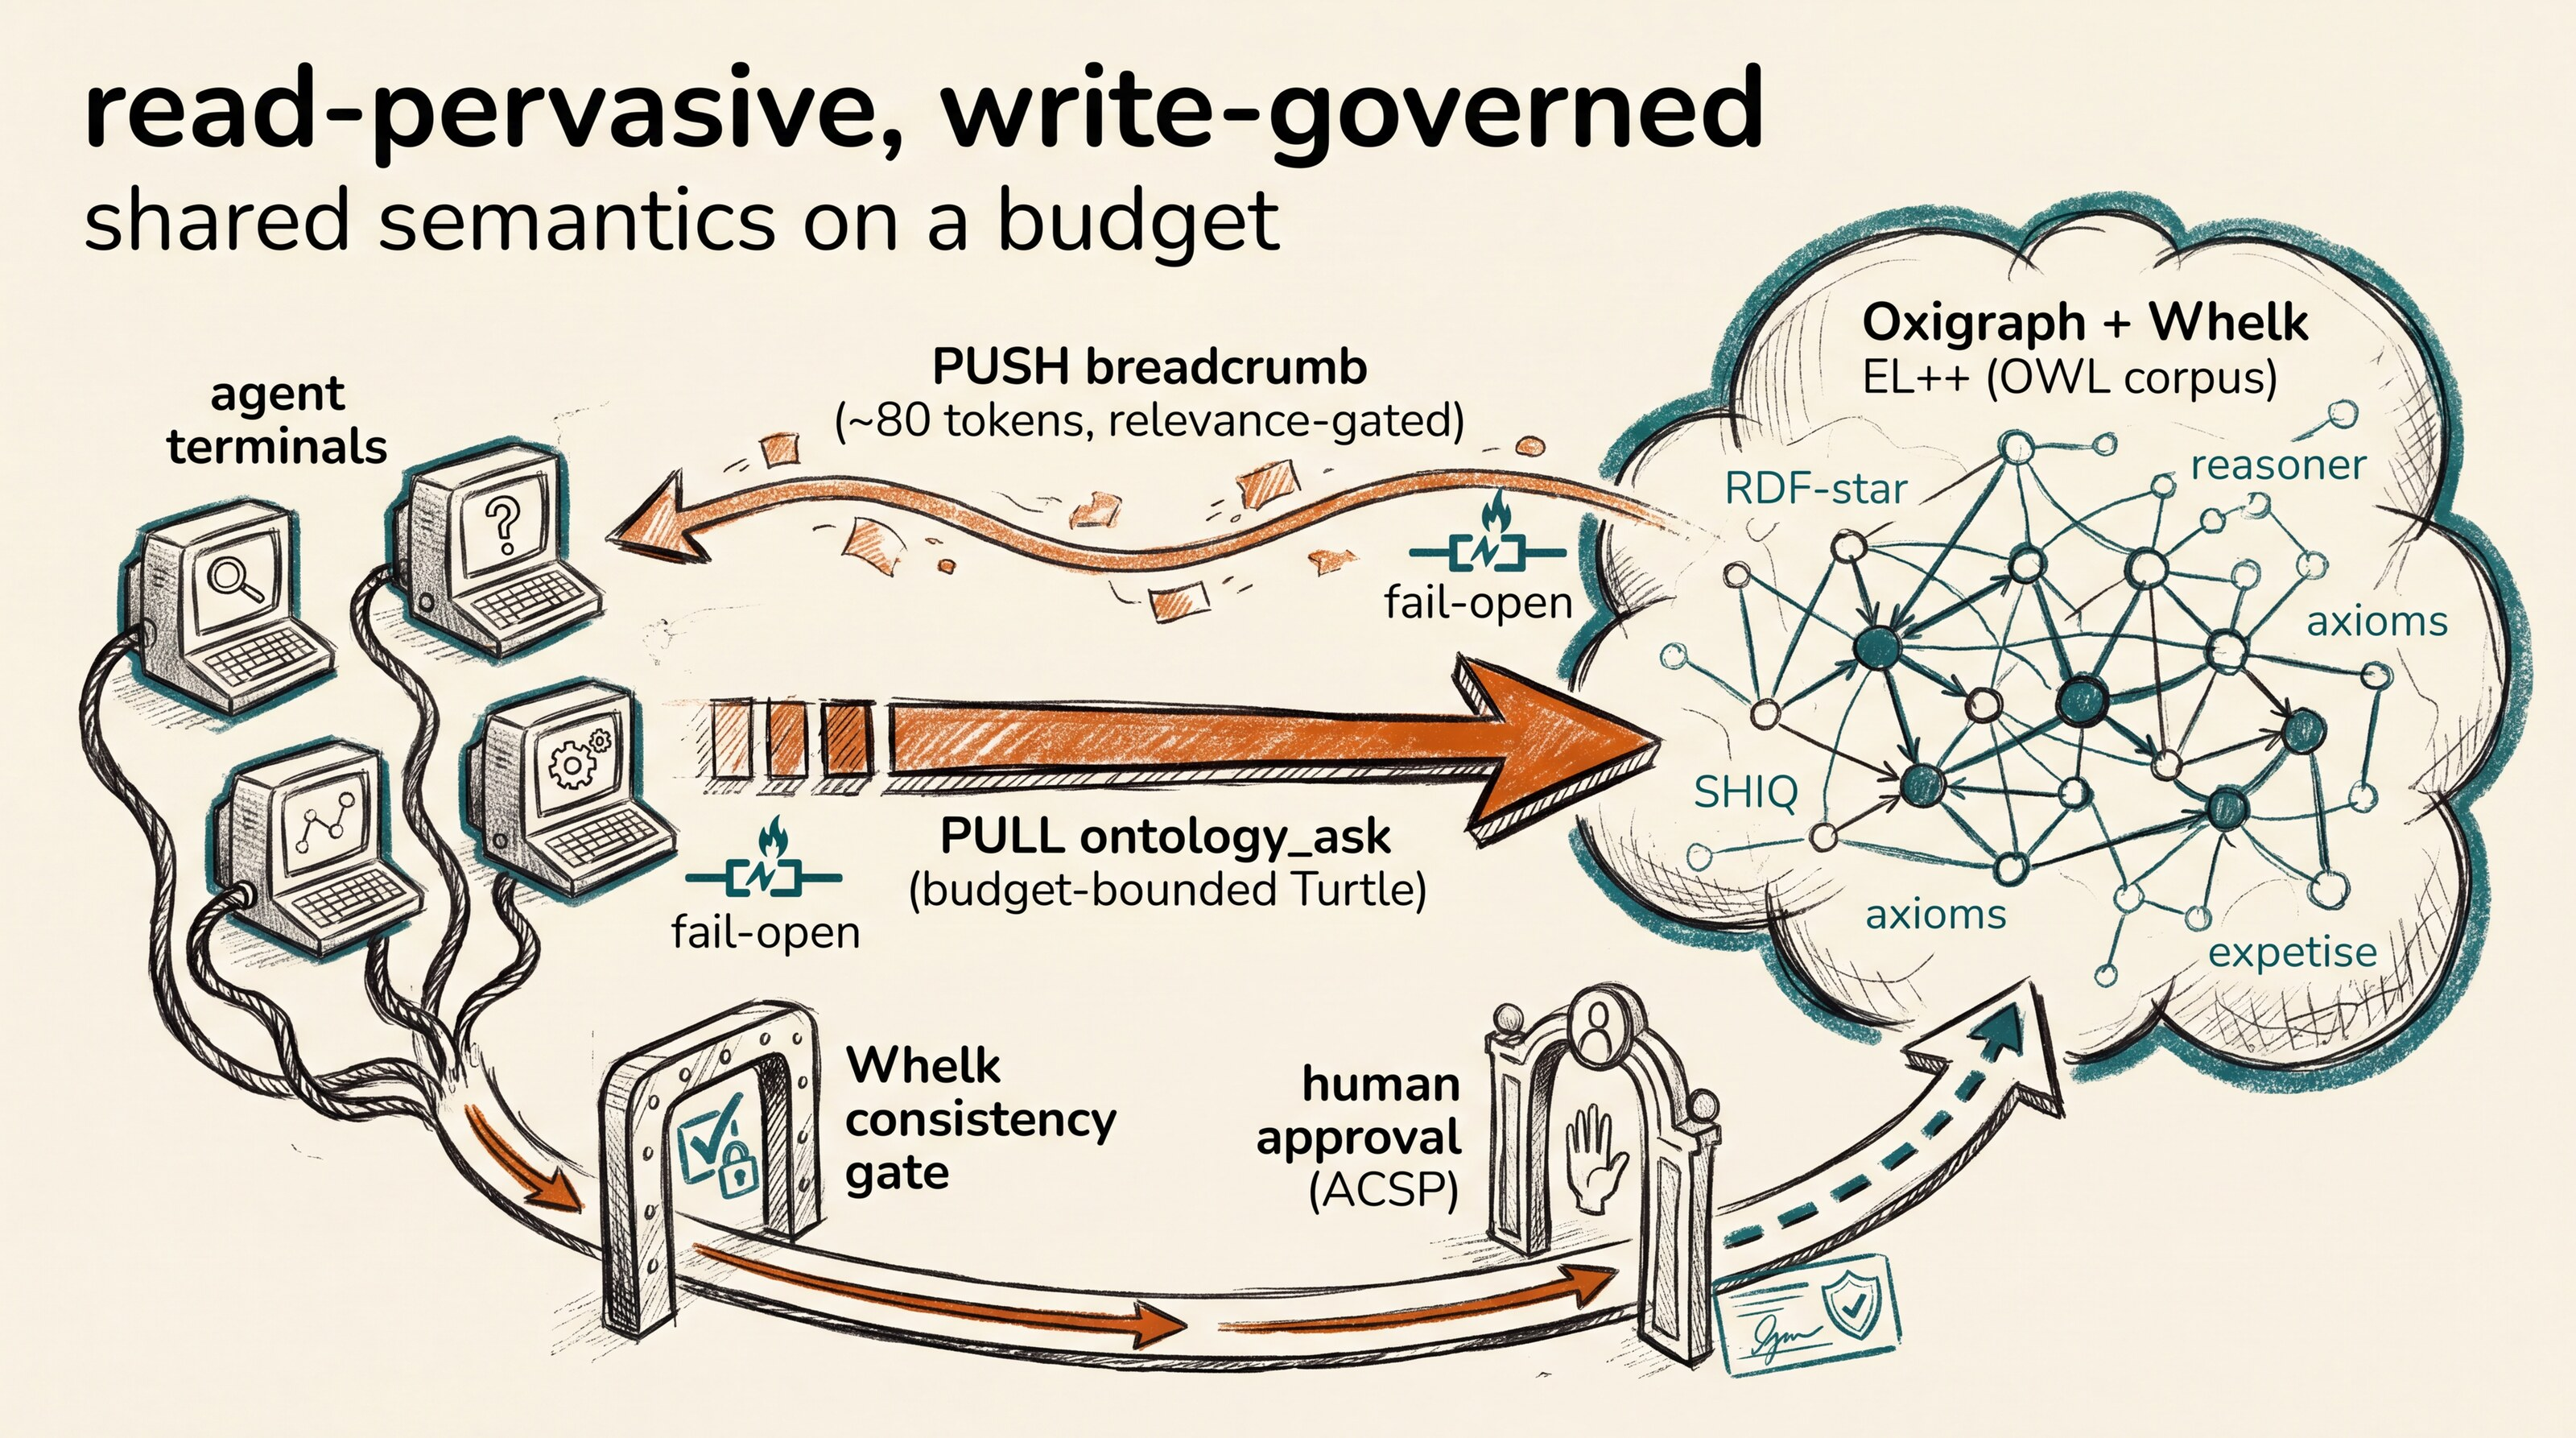
\includegraphics[width=0.92\textwidth]{nb-ontology-binding.jpg}
\caption{Two channels to shared semantics: an ambient, relevance-gated PUSH breadcrumb and a deliberate, budget-bounded PULL, with writes routed through the Whelk consistency gate and ACSP human approval. Illustration in the house sketch style.}
\label{fig:ontology-binding}
\end{figure}

\section{Read Pervasive, Write Governed}

Reading is the pervasive half. Writing is the governed half, and the asymmetry is the
whole design. The retrieval brain is read-only; it cannot mutate the graph, only survey
it. The single path to asserted truth runs through \texttt{ontology\_propose}: a proposal
is authenticated, checked by the Whelk EL++ consistency gate for logical soundness, and
then queued to the broker inbox where a human administrator signs the decision through the
forum's Agent Control Surface Protocol (Chapter~\ref{ch:forum-governance}). Derived
material an agent generates for itself (class summaries, usage telemetry) is fenced to a
\texttt{:summary} named graph; a write aimed at \texttt{:assert} or \texttt{:inferred}
is rejected server-side with a ``fenced graph'' error. Agent-derived facts stay out of the
truth layers until a human promotes them.

That asymmetry is the interface organisation \textcite{Liu2026} formalises, rendered in
code rather than in prose. Liu's account of agent collectives requires agent output to
enter a human workflow only with evidence attached and human judgment mandatory at defined
points. The chain \texttt{ontology\_propose} $\rightarrow$ Whelk consistency reasoning
$\rightarrow$ broker approval is that requirement expressed in three gates: correctness
before policy, policy before merge, evidence carried the whole way.
Chapter~\ref{ch:ecosystem-roadmap} names this same path as the one row in its findings
table that is architecture rather than aspiration.

The security of that path was a live gap through the 3 July closeout, and the gap-close
reconciliation found it already shut on main. The \texttt{propose} endpoint now requires an
authenticated principal behind a rate limit (\texttt{ontology\_agent\_handler.rs}), and the
\texttt{/api/ontology/load} backdoor that once bypassed Whelk is collapsed to a single
power-user, mutations-only scope with the weaker duplicate deleted. The sprint added a
route-guard regression test that pins both (\texttt{6f4eb1b0a}), so the front door the first
recommendation of Chapter~\ref{ch:ecosystem-roadmap} named is closed and verified rather than
merely designed (\texttt{ADR-120}). Chapter~\ref{ch:gap-register} now carries this as a closed
item rather than an open one.

\section{Fail-Open by Contract}

The binding's load-bearing promise is what happens when the backend is unreachable. Every
call is wrapped so that a backend failure degrades to an empty result and the turn
continues. A seed lookup that cannot reach the store returns \texttt{degraded:true} and
nothing else; an expand that fails after a good seed degrades to the seed menu rather than
failing the whole call. Grounding is an augmentation the agent may or may not receive,
never a dependency the agent waits on. The one discipline this imposes is interpretive: a
\texttt{degraded:true} empty result means the backend was unreachable, not that the concept
is absent, and treating the two as the same is the documented anti-pattern.

\begin{cautionbox}[title={Fail-open, observed on this book}]
This edition was itself produced with the binding in play. During one working session the
KG backend was unreachable, and every ontology call made while drafting these chapters
degraded to empty exactly as the contract specifies: no error surfaced to the turn, no
draft stalled, and the writing continued from the decision records and skill documentation
instead. The fail-open guarantee is not reported here from a test rig. It was observed in
the field, on the production of this book, and the chapter you are reading is one of the
turns that continued ungrounded when the graph went dark. A second field observation
records the same behaviour on a later date. During the July 2026 reconciliation pass for
this edition, four \texttt{ontology\_ask} calls across the book's core domains
(telepresence, distributed identity, Bitcoin value rails, and digital-society governance)
each returned \texttt{degraded:true} with \texttt{seed\_unavailable} in about four seconds,
one more logged instance of the fail-open contract holding rather than blocking the turn.
What both observations lacked at the time was a way to tell a degraded turn from a dead
binding without a human noticing the empty results; the gap-close sprint closed that blind
spot, and the next section records the monitor it added.
\end{cautionbox}

Fail-open also carries an honesty cost the book insists on paying. A silent
degrade-to-empty is indistinguishable, from the outside, from a binding that was never
wired at all. That is the exact failure an earlier workstream (\texttt{PRD-018}) shipped,
where ontology forces were compiled and inert for months because nobody proved the consumer
invoked them. The binding answers this with per-channel liveness counters and a startup
canary that drives a non-zero injection through each enabled channel and asserts it landed
(\texttt{ADR-119}): a green-but-zero dashboard is treated as failure. The gap-close sprint
extended that discipline to the knowledge-graph backend itself, which is the one dependency
the fail-open contract silently tolerates losing. Because the server is the KG backend and
its \texttt{/api/health} and \texttt{/healthz} endpoints existed but were polled by nothing,
the sprint added a watchdog that polls them and drives a \texttt{kg\_backend\_up} gauge, plus
a liveness harness that registers, observes, and re-arms canaries on a thirty-day staleness
clock, seeded with six standing P0 canaries (\texttt{6f4eb1b0a}); a companion tap maps a Nostr
kind-1 heartbeat into the same harness so an external prover can confirm liveness fail-open
(\texttt{1492bc17b}). The backend-down day recorded above would now trip the gauge rather than
pass unnoticed. The three read channels remain built and verified in the agentbox Node layer
(eighteen of eighteen unit tests passing), and the server-side workstreams the earlier edition
listed as pending the Rust host build now sit behind that live watchdog. In the governed
vocabulary of \texttt{ADR-002}, the binding is integrated on its read path, monitored at its
backend, and still hardening on its write path.

\section{One Honest Gap in the Write Path}

The governed-write story has a seam the register records, and it belongs in this chapter
rather than only in the gap register because it is the point where canon and practice
diverge most instructively. The canon commits to a clear ordering: ontology mutation
crosses a formal correctness gate before it crosses a human-policy gate, Whelk first, then
ACSP. The general agentbox \texttt{ontology\_propose} path implements that ordering. The
\emph{personal-to-shared elevation path} (the \texttt{ElevationActor} that promotes a
concept out of an individual's knowledge graph into the shared ontology) skipped
the Whelk consistency gate at the 3 July closeout (finding GOV-7): a concept could
reach the human-policy gate without first clearing the correctness gate the canon
places ahead of it. That divergence closed in code on 11 July 2026. The approve arm now
checks the base ontology unioned with the drafted axioms through
\texttt{WhelkInferenceEngine::check\_axiom\_set} and fails closed --- an inconsistent draft,
or a reasoner that cannot be constructed, records a reject and opens no PR (VisionClaw
\texttt{43a12e401}). The espoused sequence and the wired sequence now agree on both
elevation routes; the register records the closure with the candour it recorded the gap,
and the residual honesty is that the gate's blocking behaviour is proven by unit canary,
not yet by a live elevation.

The wider writeback ambition sits further out. The self-improving elevation flywheel
(\texttt{ADR-121}), the two-speed routing that would send volatile facts to a fenced
\texttt{:observed} graph while structural changes route to the human gate (\texttt{ADR-122}),
and voice-mediated sign-off (\texttt{ADR-123}) are written designs marked spec-only, and the
codebase still carries a \texttt{writeback\_triggered} flag that reports writes it never
performs, the ghost \texttt{ADR-121} exists to delete. What ships today is the read binding
and the governed single-proposal path; the flywheel that would close the loop between them
is named, specified, and frozen. Stating that altitude here is cheaper than letting a reader
find it in the code.

\chapter{DreamLab Edge: the Operator Overlay}
\label{ch:dreamlab-edge}

\epigraph{Standing up a community should cost a configuration file, not a codebase.}{}

DreamLab Edge is the branded public face of the ecosystem, the \texttt{dreamlab-ai-website} repository that renders at dreamlab-ai.com. It is the surface a visitor actually meets: a React marketing site at the origin and a Rust/Leptos WASM forum at \texttt{/community/}, both served from GitHub Pages and backed by five Rust Cloudflare Workers. Of the six substrates this Part examines, it is the one built to hold the least of its own logic. The design goal is deliberate poverty. Edge should own its branding, a handful of Cloudflare resource identifiers, and a policy of who may read which zone, and nothing more. Everything that makes the forum a forum lives upstream in the kit examined in Chapter~\ref{ch:forum-governance}.

\section{A Branded Face on a Shared Kit}

Edge consumes the \texttt{nostr-rust-forum} kit as its backend. The separation follows \texttt{PRD-012} (kit adoption) and \texttt{ADR-085} (the \texttt{forum-config} package): the five Rust workers and the Leptos client live in the kit repository, and this repository holds only an operator overlay under \texttt{forum-config/}. Continuous integration clones the kit at a pinned commit and lays DreamLab's own worker manifests over it at build time. Table~\ref{tab:edge-ownership} states the split that this arrangement enforces.

\begin{table}[h]
\centering
\caption{What the kit owns and what the operator owns}
\label{tab:edge-ownership}
\begin{tabularx}{\textwidth}{L{5.4cm} X}
\toprule
\textbf{Concern} & \textbf{Owner} \\
\midrule
Worker source; Leptos forum client & \texttt{nostr-rust-forum} kit \\
\addlinespace
Cloudflare resource IDs (D1, KV, R2, AI) & \texttt{forum-config/deploy/*.wrangler.toml} \\
\addlinespace
Branding, zones, feature flags, governance & \texttt{forum-config/dreamlab.toml} \\
\addlinespace
React marketing site; smoke and integration tests & this repository \\
\bottomrule
\end{tabularx}
\end{table}

Identity is \texttt{did:nostr} throughout, obtained by passkey, browser extension, or direct key entry. Access divides into four zones: a public MiniMooNoir landing, plus locked Friends, Family, and DreamLab-business zones. Those zones are authored once, in the \texttt{[[zones]]} tables of \texttt{dreamlab.toml}, and projected into two enforcement points that must stay in step: the relay worker's \texttt{ZONE\_CONFIG} variable gates reads and writes server-side, and the same JSON is injected into the client's \texttt{window.\_\_ENV\_\_} to render zone tiles. The Family zone is NIP-44 encrypted; the others are relay-ACL gated. A non-member sees a visible-but-locked tile rather than nothing, so the shape of the community is legible before entry.

Beneath the branding the deployment is two single-page applications on one origin. The React marketing site and the Leptos forum share dreamlab-ai.com and nothing else; the forum's five workers, for authentication, pod storage, link preview, relay transport, and semantic search, run as separate Rust WASM Cloudflare Workers. Authentication carries no password and stores no key: a WebAuthn passkey's PRF output is fed through HKDF to derive a secp256k1 private key deterministically, the key lives only inside a Rust closure and is zeroized on page unload, and every write to a worker is a NIP-98 signed request checked for replay in a shared D1 table. None of that mechanism is DreamLab's to maintain. It arrives with the kit, and the overlay selects it.

A single feature shows what config-driven policy buys. The forum's NIP-52 calendar projects each event differently per viewer cohort. An administrator and family members see full detail; a friends-cohort viewer sees redacted free/busy blocks for family and business events, carrying start, end, and a busy flag but never titles or notes; a business viewer is unaware the family and friends calendars exist at all. Table~\ref{tab:edge-calendar} states the matrix. The projection runs server-side at the relay, so redacted material never reaches an unauthorised client, and the whole visibility scheme follows from the cohort assignments authored in \texttt{dreamlab.toml}. Changing who sees what is a configuration edit, not a code change.

\begin{table}[h]
\centering
\caption{Per-cohort projection of the NIP-52 calendar}
\label{tab:edge-calendar}
\begin{tabularx}{\textwidth}{L{3.2cm} X X X}
\toprule
\textbf{Viewer cohort} & \textbf{Family events} & \textbf{Business events} & \textbf{Friends events} \\
\midrule
Administrator & full detail & full detail & full detail \\
\addlinespace
Family & full detail & full detail & full detail \\
\addlinespace
Friends & free/busy only & free/busy only & full detail \\
\addlinespace
Business & none (unaware) & full detail & none (unaware) \\
\bottomrule
\end{tabularx}
\end{table}

The kit relationship carries a licence seam as well. The branded React shell is proprietary; the forum surfaces, meaning the \texttt{forum-config/} overlay, the deployed workers, and the Leptos client, are combined works of the AGPL-3.0 kit that \texttt{forum-config} statically links, and are therefore AGPL-3.0. A visitor interacting with the forum over the network is entitled under AGPL~\S13 to the corresponding source: the pinned upstream kit plus the local overlay. This dual-licence-by-surface split is the legal shadow of the kit-and-overlay architecture. What DreamLab wrote stays proprietary, what it configures stays open.

\section{What an Operator Owns}

\begin{keyinsight}[title={A Community as a Configuration Act}]
What an operator of a DreamLab-style forum owns reduces to one TOML file and a set of deploy manifests. \texttt{dreamlab.toml} is the authored source of truth for zones, branding, feature flags, and governance parameters; \texttt{forum-config/deploy/*.wrangler.toml} carry the Cloudflare resource identifiers. To stand up a second community, an operator writes a second \texttt{dreamlab.toml} and a second set of manifests. No fork of the forum, no new client code, no new workers. The kit-and-overlay split is the ecosystem's scaling model: making a new community is a configuration act, not an engineering one, and that is precisely how a six-substrate mesh proposes to grow past the one team that built it.
\end{keyinsight}

The split is machine-checked, which is what raises it above aspiration. The kit is pinned in four load-bearing places that must move together: the \texttt{KIT\_REF} variable in each of three GitHub workflows, and the \texttt{rev} on every \texttt{nostr-bbs-*} dependency in \texttt{forum-config/Cargo.toml}. A dedicated continuous-integration dual-pin check asserts that all four agree, because bumping one alone ships a client, worker, and test skew. That guard is real and it works. The prose around it does not keep pace: the repository's two README files quote two different, stale kit revisions (\texttt{25ca8a1} in one, \texttt{3c16c21} in the other) while the enforced pin is \texttt{a149da4}. Machine-synchronised config, documentation that drifts around it. Owning almost nothing still leaves prose to rot, and a chapter committed to the honest version records the rot rather than the README.

The overlay also ships the means to prove a deployment behaves. \texttt{forum-config} carries a suite of seed and probe scripts an operator runs against the live four-zone deployment. One seeds the whole fixture: whitelisting tier users into cohorts, posting a message as each tier to validate the write gates, and publishing calendar events that exercise the projection matrix above. Others probe NIP-42 AUTH and zone reads, the per-tier calendar projection, and pod conditional-request handling. The admin key is read from the environment and never printed. The overlay owning its own verification is the right boundary: the kit proves the kit, the operator proves the deployment.

That honesty extends to the config's own rough edges, stated in place rather than hidden. The \texttt{[admin]} section currently lists the \texttt{visionclaw-server} key as the primary forum administrator, even though \texttt{forum-config}'s own identity roster documents that same key as a non-admin service identity whose job is to publish governance panels. It stays there only to remain in lockstep with the pubkey mirrored into the relay, search, and auth workers' \texttt{ADMIN\_PUBKEYS}, which a continuous-integration check requires to agree; removing it in one place alone would split the admin set. A standing \texttt{TODO} in the file records that a dedicated admin keypair should replace it. A service identity doubling as the top human administrator is the kind of expedient a thin overlay accretes precisely because it owns so little, and writing it down costs less than pretending it is absent.

\section{Where the Cutover Stands}

Edge is live as a deployment and, as an independent artefact, the earliest-stage of the six. Those two facts describe different moments, and the distance between them is the de-specialisation still in flight. The overlay exists (Phase X3 in \texttt{PRD-012}): the legacy in-repository forum \texttt{community-forum-rs} has been renamed \texttt{community-forum-rs.frozen} and is pending deletion, but the route-level cutover from legacy workers to the overlay workers has not happened. Phase X4 waits on the kit exposing a \texttt{nostr-bbs-*-worker::dispatch} extension API; until it lands, \texttt{forum-config/src} carries per-worker entry shims that stand in for a dispatch surface the kit does not yet publish. So the clean thin-consumer separation that this chapter describes as the model is a target the codebase is refactoring toward, not a finished state. In the governed maturity vocabulary of \texttt{ADR-002}, Edge runs as a live deployment while sitting short of \emph{federation-verified} as a component in its own right. Recommendation~12 of Chapter~\ref{ch:ecosystem-roadmap} ties completing this cutover to the first pilot of the stack outside DreamLab.

\section{Declared, Dark Federation}

One small fact is worth stating precisely, because it sits on the ecosystem's outward edge. The overlay declares relay federation configuration that it does not exercise. \texttt{dreamlab.toml} carries a full \texttt{[mesh]} block: peer relay URLs, a \texttt{federated\_kinds} allow-list that includes the governance kinds 31400--31405, an \texttt{allowed\_remote\_dids} roster of trusted peers. Yet \texttt{mode} is \texttt{standalone} and \texttt{peer\_relays} is empty, so none of it fires. The relay is loopback in practice; the deployment reaches its own backend over HTTPS and WSS to Cloudflare Workers, and as a GitHub Pages and Workers deployment it cannot join a Tailscale tailnet at all. The federation block is present, complete, and dark.

Edge participates in two of the ecosystem's three federation transport strata, and cannot reach the third. Table~\ref{tab:edge-transport} states which and why. Its relay worker bridges browser clients to the Nostr relay, and, when the \texttt{[native\_pod]} section is enabled, its auth worker forwards pod provisioning to an agentbox-hosted \texttt{solid-pod-rs} server (Chapter~\ref{ch:solid-pod}) through a Cloudflare Tunnel. A Tailscale tailnet is closed to it outright, because a GitHub Pages and Workers deployment has no host on which to run the tailnet daemon.

\begin{table}[h]
\centering
\caption{Edge across the three federation transport strata}
\label{tab:edge-transport}
\begin{tabularx}{\textwidth}{L{3.4cm} L{4.0cm} X}
\toprule
\textbf{Stratum} & \textbf{Edge participation} & \textbf{Reason} \\
\midrule
1: Tailscale tailnet & Not applicable & GitHub Pages and Workers cannot join a tailnet \\
\addlinespace
2: Nostr relays & Relay worker (Durable Objects) & Browser-to-relay bridge; governance kinds surface in the forum \\
\addlinespace
3: Cloudflare Tunnel & Auth worker, when \texttt{[native\_pod]} is enabled & Reach the agentbox-hosted native pod tier \\
\bottomrule
\end{tabularx}
\end{table}

The reason this matters more than a dormant config stanza usually would: relay federation is where the six substrates would pass governance events to one another, the point at which agentbox and VisionClaw governance panels reach the forum a human reads. The declared \texttt{[mesh]} block (\texttt{PRD-010} Phase 3, \texttt{ADR-073}) is a promise the wire does not yet keep, populated only when peers come online. A thin consumer inherits both the kit's economy and the kit's overstatements, and Edge inherits one worth naming: the relay it renders describes its gate as NIP-42 AUTH, while the code-verified behaviour is a pubkey allowlist with \texttt{auth\_required} set false, a whitelist check rather than a full AUTH round-trip. Closing that overstatement before the relay is ever exposed to peers is exactly the security front-loading that distinguishes deployments which compound from those which stall \parencite{Pereira2026Playbook}. The gap belongs to the forum kit and is catalogued in Chapter~\ref{ch:gap-register}; Edge carries it forward because carrying the kit forward is its whole job.

\begin{cautionbox}[title={What Edge Is Not Yet}]
\begin{itemize}
  \item Live as a deployment, but the earliest-stage of the six as an independent artefact: the thin-consumer separation is a refactor in progress, not a shipped state.
  \item The \texttt{PRD-012} cutover is mid-flight. The legacy forum is frozen and pending deletion; the D2 route handover waits on a kit dispatch API that does not yet exist.
  \item Relay federation is declared and dark. The \texttt{[mesh]} block is authored in full but runs \texttt{standalone}, so no governance event crosses to a peer today.
\end{itemize}
\end{cautionbox}

Edge is the ecosystem's answer to the question every other chapter defers: how does any of this reach a second team? The answer offered here is to make standing up a community a matter of writing one configuration file, so that the marginal cost of the next deployment is closer to editing a TOML than to running a project. That answer is only half-delivered while the cutover is unfinished and the mesh block runs dark, and this report records both the design and the honest distance still to close.


\part{An Honest Assessment}
\label{part:assessment}

\chapter{The Gap Register: Theory Meets Practice}
\label{ch:gap-register}

\epigraph{A capability you have built but cannot see acting is, to the person who needs it, indistinguishable from one you never built.}{}

Chapter~\ref{ch:ecosystem-roadmap} committed DreamLab, in print, to running its own prescriptions on its own systems. This chapter supplies the measurement that makes such a commitment falsifiable. It reports a systematic audit of the four surfaces through which humans and agents actually meet in the VisionClaw ecosystem: the async governance forum, the desktop 3D client, the mixed-reality headset, and voice. This audit is scored against both what the canon promises and what the published research says a collaboration surface must do. The finding, stated plainly before the detail: the substrate is stronger than the interaction. Real cryptographic governance and a designed identity spine sit underneath surfaces on which, today, an operator can watch a count and fire a form, and little else.

\section{How the register was built}

The four surfaces are the ones defined and weighted in Chapter~\ref{ch:four-surfaces}. Each received the same treatment from a twelve-agent \meshterm{analysis mesh}: one agent extracted the canon (what the README, the ADR and PRD corpus, and the 2026-07-03 closeout files actually claim); four surveyed the shipping code, one per surface, recording every capability as \emph{working}, \emph{partial}, \emph{scaffolded}, \emph{absent} or \emph{docs-only} against the governed maturity vocabulary of \texttt{ADR-002}; three researched the human-computer-interaction and multi-agent literature on independent search engines, so no single index shaped the theory; and four adversarial judges, one per surface, ranked each surface's canon and code against that literature. Findings were weighted 40/30/20/10 across forum, desktop, mixed reality and voice, matching the weighting fixed in Chapter~\ref{ch:four-surfaces}: the forum carries the governance load, so it carries the most scrutiny.

Every gap is typed by where the break sits, because the remedy differs by type.

\begin{definitionbox}[title={Three kinds of gap}]
\begin{description}[style=nextline, leftmargin=1.5em]
  \item[Theory-to-canon] Published knowledge our own documents never adopted. The fix is a design position, written down.
  \item[Canon-to-practice] Our documents promise a capability the code does not deliver. The fix is engineering, or an honest retraction of the claim.
  \item[Theory-to-practice] Nobody wrote it down and the code lacks it. The fix is both.
\end{description}
\end{definitionbox}

The register holds 28 gaps: 7 rated critical, 17 major, 4 minor. Those counts are reported here exactly as the judges set them, without rounding or dramatisation. Strengths were recorded with the same discipline, and two of them matter to the argument as much as any gap: relay-enforced separation of who may ask from who may decide, and a cryptographic \texttt{did:nostr} agent identity, both of which sit ahead of common 2026 industry practice, against a landscape in which deployed agent governance and self-disclosure are documented as inconsistent and frequently absent \parencite{AgentIndex2025}.

A note on the honesty of the exercise. The auditor and the audited are the same organisation, and selection bias cuts both ways: an author examining their own system may be harsher than an outsider, or blinder. The register mitigates this by tying every gap to a file and line the reader can open, and by scoring against external literature the authors did not write. It does not eliminate the conflict, which Chapter~\ref{ch:open-questions} names directly. The register is offered as a checkable claim, not a verdict.

\section{Forum: a governance plane for one operator}

The forum is the ecosystem's one production human-in-the-loop mechanism, and its foundations are genuinely good. The Agent Control Surface Protocol (ACSP, Nostr kinds 31400--31405) is wired end to end: an agent publishes a signed \texttt{PanelDefinition} or \texttt{ActionRequest} only after an admin has provisioned it atomically into the \texttt{agent\_registry} (\texttt{ADR-097}), and a human approval is a real signer-backed kind-31403 event, not a UI toggle. The relay is the sole enforcement point, so a non-admin who reaches an Approve button still has the event rejected server-side (\texttt{nip\_handlers.rs:360-368}). That defence-in-depth posture, plus content-addressed decisions aligned with the PROV-AGENT direction of provenance research \parencite{Souza2025ProvAgent}, is the substrate for a real audit trail. What sits on top of it is narrower than the canon advertises.

\begin{table}[h]
\centering
\caption{Forum surface: 10 gaps (2 critical, 7 major, 1 minor)}
\label{tab:gaps-forum}
\begin{tabularx}{\textwidth}{X L{3.2cm} L{1.6cm}}
\toprule
\textbf{Gap} & \textbf{Type} & \textbf{Severity} \\
\midrule
Governance plane is admin-only, excluding ordinary humans & canon-to-practice & Critical \\
\addlinespace
No agent disclosure: agents indistinguishable from humans & theory-to-practice & Critical \\
\addlinespace
Decisions binary; graduated-escalation lifecycle is dead code & canon-to-practice & Major \\
\addlinespace
Forum-client decisions optimistic-only; a rejected decision reads as sent & canon-to-practice & Major \\
\addlinespace
No trust-calibration context at decision time; no decision-audit read API & theory-to-practice & Major \\
\addlinespace
No revoke, appeal or supersede authority for a published decision & theory-to-canon & Major \\
\addlinespace
No design response to approval fatigue / automation complacency & theory-to-canon & Major \\
\addlinespace
No web UI for agent-roster administration & canon-to-practice & Major \\
\addlinespace
Cross-relay federation of governance events absent & canon-to-practice & Major \\
\addlinespace
Silent on multi-agent social influence in threads & theory-to-canon & Minor \\
\bottomrule
\end{tabularx}
\end{table}

The most serious finding is that this is an operator-in-the-loop plane, not a community one. The forum-client \texttt{/governance} route is wrapped in \texttt{AdminGatedGovernance}, which bounces any authenticated non-admin to \texttt{/forums} with a toast before the governance page ever mounts (\texttt{app.rs:1135-1143}), and the relay hard-gates kind-31403 responses to admins. The canon's \texttt{architecture.md} Trust and Gating table explicitly grants members the right to view panels; the shipping code shows them nothing. The flagship chokepoint the canon renders in every scenario as ``Forum $\rightarrow$ Human decides'' is, in the product, ``Forum $\rightarrow$ Admin decides,'' and the distributed-judgment claim collapses to a single-operator approval queue. This directly undercuts the ambient-awareness model the canon leans on, in which coordination depends on shared-workspace visibility \parencite{DourishBellotti1992}.

The second critical gap is disclosure. Agent public keys resolve through the identical display-name cache used for every human member, with no bot badge anywhere in either client (\texttt{governance.rs:134-135}, \texttt{user\_display.rs}). An ordinary reader cannot tell an agent from a human at the point of reading its output or its governance panel. This is the one place the external literature is unanimous: the agentic web requires agents to identify themselves and their authorising principal \parencite{AgenticWebNorms2026}, and deployed practice remains inconsistent enough that disclosure failures have already produced public scandals \parencite{AgentIndex2025}. The canon names agents as distinct \texttt{did:nostr} subjects but requires no visible disclosure, and neither does the code.

The seven major forum gaps compound the two critical ones. The decision model is binary in practice. A fully unit-tested \texttt{DecisionOrchestrator} with delegate, promote and precedent transitions exists in \texttt{nostr-bbs-core}, but it is referenced only inside its own test module, and the live relay projection maps only approve to resolved and reject to rejected, parking any other action in \texttt{under\_review} permanently (\texttt{nip\_handlers.rs:1316-1320}). Both the external consensus on risk-tiered graduated delegation \parencite{Tomasev2026Delegation} and the ecosystem's own richer domain model exceed what ships, and \texttt{architecture.md} documents the unreachable lifecycle as if it were live.

Forum-client decisions are optimistic-only. \texttt{PanelCard} fires a fire-and-forget \texttt{relay.publish()} and flips the UI to ``sent'' the moment local signing succeeds, before any NIP-01 acceptance frame returns (\texttt{governance.rs:206-221}). Because the relay independently rejects non-admin and other invalid events, a user can believe they governed an agent action when nothing was accepted. This false-positive success signal miscalibrates trust exactly where calibration matters most. The sibling BBS client already does this correctly with \texttt{publish\_with\_ack}.

At the decision moment the human is shown title, description and buttons, but no reasoning trace, confidence, risk tier or provenance, and there is no \texttt{GET /api/governance/decisions} read path to review precedent afterwards. A gap the repository documents against itself as Finding 5. Exposing reasoning and disagreement, rather than only a final ask, is what the calibrated-trust literature identifies as the precondition for appropriate reliance \parencite{TrustingTeammates2025}, and reliability does not scale with capability, so per-request evidence is not optional.

Three further major gaps are governance omissions the canon never resolved. There is no revoke, appeal or supersede path: the domain model declares a decision immutable, correctable only by a superseding event, yet neither canon nor code specifies who may publish that event or under what authority, leaving an operator who approves in error with no defined recourse against a settled decision that interruptible-agent research treats as a routine need \parencite{Interruptible2026}. The canon frames governance as an accelerant while offering no safeguard against the accelerant becoming a rubber stamp: a single admin facing an undifferentiated stream of binary panels is the textbook trigger for the approval fatigue and automation complacency the empirical record identifies as the first oversight mechanism to fail \parencite{AutomationBias2012}.

The single most authority-laden act, deciding who may act as a governing agent and revoking them, lives entirely outside the product. None of the nine governance REST endpoints is called from any forum-client page, the admin panel carries Channels, Users, NativePods and DangerZone tabs but no Agents tab (\texttt{admin.rs:108-826}), and operators provision agents through \texttt{curl} and the \texttt{dreamlab.toml} roster, precisely the out-of-band configuration the community-moderation literature warns makes bot authority illegible \parencite{Kuo2026Botender}. Cross-relay federation is absent: \texttt{nostr-bbs-mesh} is scaffold-only with zero agent references and is not a dependency of the relay worker, no 38xxx federation handler exists anywhere, and each community's governance plane is therefore an island against a canon that commits to federated substrates. The minor gap rounds out the register: the canon is silent on the emergent social influence of several agents co-present in one thread, a measurable effect given the live six-agent DreamLab roster \parencite{Song2025SocialGroups}.

\section{Desktop: embodiment that never reaches the screen}

The desktop client is the designated observation layer: humans watch here, they judge in the forum. Its bones are strong. The \texttt{ADR-059} embodiment transport is built end to end, from ingest WebSocket through the \texttt{AgentBeamActor} to a binary broadcast and a mounted client render layer, and real live agent data exists server-side, where \texttt{AgentMonitorActor} polls the agentbox Management API for genuine task statuses. The module docstrings that name the deferred gluon force and give a concrete follow-on design model engineering honesty most observability tooling does not meet. Yet almost nothing reaches the screen.

\begin{table}[h]
\centering
\caption{Desktop surface: 8 gaps (2 critical, 5 major, 1 minor)}
\label{tab:gaps-desktop}
\begin{tabularx}{\textwidth}{X L{3.2cm} L{1.6cm}}
\toprule
\textbf{Gap} & \textbf{Type} & \textbf{Severity} \\
\midrule
Embodiment channel inert: live agent activity never reaches the screen & canon-to-practice & Critical \\
\addlinespace
No steering, interruption or approval affordance in the running client & theory-to-practice & Critical \\
\addlinespace
No client-side ACSP case surface; pending judgment invisible in-scene & theory-to-canon & Major \\
\addlinespace
Agent nodes keyed by \texttt{task\_id}, not \texttt{did:nostr} & canon-to-practice & Major \\
\addlinespace
Fabricated ``MCP Connected'' status miscalibrates trust & canon-to-practice & Major \\
\addlinespace
Push-to-talk globally scoped, not directed at a selected agent & canon-to-practice & Major \\
\addlinespace
No pre-action intent legibility; embodiment shows only the past & theory-to-canon & Major \\
\addlinespace
No swarm-level observability layer versus 2026 AgentOps table stakes & theory-to-practice & Minor \\
\bottomrule
\end{tabularx}
\end{table}

The surface's entire reason to exist is inert. The beam pipeline is wired transport-to-render, but its source-position resolver and the agent-avatar renderer both read \texttt{/api/bots/agents}, whose polling loop starts only inside \texttt{BotsClient::start\_polling()}, reachable only via \texttt{BotsClient::connect()}; this call exists nowhere in the boot path (\texttt{bots\_client.rs:111,144} against \texttt{app\_state.rs:1055}). The resolver therefore always returns false, beams never draw, and the avatar layer additionally discards the real \texttt{.nodes} payload that \texttt{AgentMonitorActor} does produce. Running agents are invisible on screen. This is a live-versus-mock legibility failure rather than a mock-data problem: a dead wire returning an empty array, one missing \texttt{connect()} call away from working, while the 2026-07-03 closeout claims the beam actor is ``wired at boot.'' Continuous passive visibility of activity in the shared space is the bedrock requirement for any oversight surface \parencite{DourishBellotti1992, Epperson2025Debugging}, and the closeout claim should be downgraded to ``transport wired, position source unstarted.''

The second critical gap is that no steering, interruption or approval affordance is reachable in the running client. \texttt{AgentDetailPanel} and \texttt{BotsControlPanel} are complete but imported nowhere, and \texttt{AgentDetailPanel} additionally posts to \texttt{/bots/submit-task} and \texttt{/bots/task-status} routes that do not exist server-side. The mounted command box changes only view and physics settings. Against the dominant 2025--2026 pattern of graduated, interruptible autonomy with checkpoint-reset \parencite{Epperson2025Debugging}, the operator watching agents work cannot pause, redirect or veto anything in-scene; the actual loop is fire a form, then wait. This falls into a hole between forum and desktop, because the canon assigns in-flight steering authority to no surface the operator actually watches.

Five major gaps sharpen the picture. No client-side ACSP case surface exists: the server genuinely produces kind-31402 cases and consumes kind-31403 decisions over the forum relay, but a grep of the client for the governance kinds returns zero hits, so an escalation the server just raised is invisible until the human context-switches to a separate app. In-context escalation is what mixed-initiative theory requires so the operator can act inside the cost-of-interruption window \parencite{Horvitz1999Principles}, and the canon never assigns even an ambient pending-case indicator to the surface the operator is actually watching.

Agent nodes are keyed by ephemeral \texttt{task\_id}, not \texttt{did:nostr} (\texttt{bots\_client.rs:14-39}). Because they carry no key, they cannot be addressed by ACSP nor targeted by voice, and the canonical ``one identity across every boundary'' claim is unrealised precisely on the surface where an operator would select an agent \parencite{AuthenticatedDelegation2025}. The identity spine exists in design and is not the addressing primitive here.

The one health signal on the surface is fabricated. \texttt{get\_status()} sets \texttt{connected = true} unconditionally (\texttt{bots\_client.rs:212}) and never calls the \texttt{test\_connection()} that sits at line 231, so the green ``MCP Connected'' dot polled every three seconds reads healthy while the backend is down. This is a direct violation of the \texttt{ADR-002} maturity-honesty rule and the opposite of the honesty the same codebase models in its gluon-deferral comment; a status decoupled from ground truth drives over-reliance exactly when intervention is needed. The fix is one line.

Push-to-talk is well-built but globally scoped, routing to a generic command pipeline with no concept of a selected agent as target, blocked upstream by the same missing \texttt{did:nostr} keying. The last major gap is a canon omission: embodiment renders only what already happened, so beams show that an agent touched a node but never what an agent is about to do, and with no plan-preview or intent overlay the human can react to consequences without pre-empting them, forgoing the intervention window that intent-legibility practice targets \parencite{Nielsen2025Intent}. A minor gap notes that against the swarm-observability baseline now shipping industry-wide \parencite{AgentOps2024}, the operator gets a count and a fabricated health dot, though the underlying per-task data already exists server-side and is merely unsurfaced.

\section{Mixed reality: presence without identity}

The headset is more built than earlier gap maps implied. A user can enter an immersive session, see the live knowledge graph rendered by the same \texttt{GraphManager} the desktop uses, see live agent nodes fed by real telemetry, watch embodiment beams, and grab and drag generic nodes through a real WebSocket round-trip. The cryptographic identity designed into the wire schema is again ahead of a still-draft industry standard. Past observation, the surface is a one-directional window.

\begin{table}[h]
\centering
\caption{Mixed-reality surface: 6 gaps (2 critical, 3 major, 1 minor)}
\label{tab:gaps-mr}
\begin{tabularx}{\textwidth}{X L{3.2cm} L{1.6cm}}
\toprule
\textbf{Gap} & \textbf{Type} & \textbf{Severity} \\
\midrule
Identity-blind: agent nodes carry no \texttt{did:nostr}, no in-headset actor verifiable & canon-to-practice & Critical \\
\addlinespace
No agent-interaction or governance affordance reachable in MR & theory-to-canon & Critical \\
\addlinespace
Embodiment/copresence theory unrepresented (no avatar, gaze, proxemics) & theory-to-canon & Major \\
\addlinespace
Input layer broken: targeting ray at world-origin, gaze absent & canon-to-practice & Major \\
\addlinespace
Voice PTT-to-actor binding is complete code with zero consumers & canon-to-practice & Major \\
\addlinespace
\texttt{enterVR()} never sets \texttt{isXRMode}; XR rendering runs as desktop & canon-to-practice & Minor \\
\bottomrule
\end{tabularx}
\end{table}

The surface is identity-blind. The \texttt{Agent} struct carries \texttt{id}, name, type, status, position, health and workload, and no public-key or DID field (\texttt{bots\_client.rs:15-38}); the wire schema reserves the identity fields but marks them optional until a later phase. A headset user watching a beam has no cryptographic way to know which actor performed the action, so the canon's central trust primitive is absent exactly where embodiment makes actions visible, and ``the graph IS the audit trail'' does not hold in MR against the disclosure-and-registry direction of provenance research \parencite{Souza2025ProvAgent}. The second critical gap is that no agent-interaction or governance affordance is reachable at all: there is zero import of any command or detail panel anywhere under \texttt{client/src/immersive}, and ACSP has no client dispatcher, so a user can see agents act but cannot inspect, steer, approve or command anything from within the headset. Even a monitoring surface needs a legible intervention path \parencite{Epperson2025Debugging}, and the canon treats XR as pure rendering rather than assigning it one.

The three major gaps follow from those two. Copresence theory is unrepresented: agents render as graph nodes with no avatar, gaze or proxemic semantics, and the multi-user avatar renderer and Vircadia presence bridge exist as code but are never instantiated (\texttt{autoConnect=false}), so the one surface where spatialised copresence is native uses a desktop-2D mental model at room scale, forgoing the trust and legibility that spatial embodiment materially changes \parencite{Schmid2024Objects}. The severity is sharpened by provenance: this is a regression against the author's own quantified 2022 design brief, which fixed the gaze-offset tolerances and turn-passing costs a credible copresence system must respect \parencite{OHare2022Convergence}. These constructs are not merely unmet 2024 standards; they are the operator's own published numbers, unimplemented on the operator's own surface.

The input layer that would support in-headset steering is broken. The agent-targeting ray in \texttt{VRAgentActionScene} never receives a real XR pose and so originates at world-origin, its select callback is never wired through \texttt{VRGraphCanvas}, hand-tracking sets \texttt{isTracking}/\texttt{isPointing} booleans only with a code comment conceding it ``would need XRFrame to get actual pose,'' and gaze is entirely absent. Every downstream step (scoped command, ACSP request, voice binding) is therefore built on a selection that does not work \parencite{SpeakStaySilent2026}.

Voice push-to-talk and the LiveKit service are complete, well-written classes with zero consumers, survivors of a July 2026 dead-code pass that deleted 44 sibling orphans; even wired, they would sit atop the two broken preconditions above. The minor gap is a silent state defect: the working VR entry point never flips \texttt{isXRMode}, so XR-conditional rendering runs in desktop mode throughout a live session, invisible at the documentation layer and surfacing only on-device.

\section{Voice: one closed loop, narrowly scoped}

One genuine end-to-end voice loop exists, and it is honestly the best-behaved thing in the register. \texttt{VoiceInterfaceActor} (\texttt{ADR-110}) subscribes at boot to the Whisper transcription broadcast, gates on a conservative verb-plus-noun grammar, routes to the same settings-assistant LLM the typed control centre uses, and confirms aloud through Kokoro TTS. That is a real human-speaks, agent-hears, agent-responds-by-voice turn, with two strengths that exceed industry practice: identity is asserted from the operator's configured key and never from the transcript (``a transcript cannot assert an identity it does not hold''), and an unrecognised utterance falls back to a read-only query rather than a silent mutation. The loop is scoped to interface tweaks, not agent dialogue or governed action.

\begin{table}[h]
\centering
\caption{Voice surface: 4 gaps (1 critical, 2 major, 1 minor)}
\label{tab:gaps-voice}
\begin{tabularx}{\textwidth}{X L{3.2cm} L{1.6cm}}
\toprule
\textbf{Gap} & \textbf{Type} & \textbf{Severity} \\
\midrule
Canonical PTT voice-to-selected-actor governed-action loop does not exist & canon-to-practice & Critical \\
\addlinespace
No multi-agent addressing or turn-taking model & theory-to-canon & Major \\
\addlinespace
No conversational grounding or repair & theory-to-canon & Major \\
\addlinespace
Docs describe a deprecated voice-to-swarm path as live & canon-to-practice & Minor \\
\bottomrule
\end{tabularx}
\end{table}

The canon documents push-to-talk capturing the selected agent node and dispatching a scoped, signed ACSP request to that agent's \texttt{did:nostr} as step one of its flagship journey. No wired path connects live speech to a selection-aware, signed, addressed agent action. The one producer built for it, agentbox's \texttt{/v1/voice-intent}, is gated off by default (\texttt{agentbox.toml:34}), accepts only a flat optional actor string with no scene-selection binding, and has zero callers in VisionFlow's own STT pipeline; the addressing key it would need does not exist, because agent nodes remain \texttt{task\_id}-keyed \parencite{AuthenticatedDelegation2025}. The canon prose for this step notably lacks the file-and-line evidence that surrounds every genuinely shipped claim elsewhere in the same document.

The two major gaps are theory the canon never adopted. Nothing tells the human which agent is listening: awareness cues are one-directional, two competing swarm-keyword paths fire on the same audio with no floor management, and multi-party addressing has no convention here at all \parencite{SpeakStaySilent2026}. There is no grounding or repair move: unrecognised speech degrades to silence or a read-only default, never a clarifying question, exactly the failure the grounding literature names as central for voice agents, which issue repair requests far less often than humans do \parencite{GroundingRifts2025}. The minor gap is documentation drift: the how-to still describes a voice-to-swarm path that the code has actively deprecated to a canned ``use REST API instead.''

\section{Four surfaces, four recurring patterns}

Read across the surfaces, the 28 gaps resolve into four patterns, and the pattern is more instructive than any single gap.

First, the mesh acts but cannot yet be seen acting. The desktop beam pipeline is complete and inert, the MR surface renders beams without a verifiable actor behind them, and no surface offers the swarm-level observability that is now table stakes. Real agent activity exists server-side on every surface and reaches the operator's eye on none. This is the signature failure of the whole register: capabilities built to the point of one missing wire, then left unstarted.

Second, the identity spine is strong at rest and unused in interaction. The \texttt{did:nostr} identity is designed into the provisioning path, the relay gating and the wire schema, and it is ahead of a still-draft industry standard \parencite{AIIdentity2026}. At the point of interaction it disappears: agent nodes are keyed by \texttt{task\_id} on desktop, on MR and in voice, so the one identity that is meant to cross every trust boundary is never the addressing primitive on any surface where a human would select an agent. Three separate gaps (ACSP addressing, voice targeting and MR verification) share this single root.

\begin{keyinsight}[title={The register's through line}]
The ecosystem's failures are rarely ``it does not work.'' They are ``it is built, and unwired.'' A cryptographic identity that is never read at interaction time; a governance plane real enough to reject a forged approval yet open to only one operator; a beam transport complete to the last actor and starved by an absent \texttt{connect()} call. The distance between the substrate and the surface is the distance this edition asks to be measured on.
\end{keyinsight}

Third, governance is real but admin-only. The forum enforces, at the relay, who may ask and who may decide, an achievement most deployed agent systems lack. It also confines every decision to a single administrator role, with a binary control, no risk-tiering, no disclosure of the deciding actor, and no appeal. Distributed human judgment, the report's own premise, collapses to a single approval queue that the automation-complacency literature predicts will be the first thing to fail.

Fourth, every surface's voice story ends at the same unconsumed binding. Desktop push-to-talk is globally scoped; MR push-to-talk has zero consumers; the voice surface's flagship loop is gated off and uncalled. All three block on the identical pair of missing preconditions, \texttt{did:nostr}-keyed agent nodes and a working selection, so what looks like four independent voice gaps is one unbuilt binding seen from four angles. The type distribution says the same thing another way: of the 28 gaps, the largest class is canon-to-practice, documents promising what the code does not yet deliver. That is a more recoverable position than a system whose theory is wrong, and a more embarrassing one to leave standing in print.

\section{Handing off to remediation}

This chapter measures; it does not prescribe. The remediation sits in Chapter~\ref{ch:ecosystem-roadmap}, and the mapping is close to one-to-one. The roadmap's first priority, closing the governed-writeback security gaps, must precede everything the forum register flags. Surfacing the broker case queue inside the client answers the desktop ``no ACSP surface'' gap and the forum ``admin-only, binary'' gaps together. Threading a \texttt{did:nostr} onto agent nodes is the shared unblocker for the identity-spine pattern across desktop, MR and voice.

Chapter~\ref{ch:open-questions} then takes up the gaps that no engineering ticket closes: the ones where the canon itself is silent and the theory is unsettled, from multi-human decision conflict to XR-specific consent. This chapter's job was narrower and prior to that one. It fixed the numbers. Whether those commitments are met, or conspicuously not met, is what the next edition will report against this register, which is the point of stating the counts, the file paths and the severities exactly, now, before the work is done.

\section{One sprint later}

The audit above is the historical record, and it stands unedited: the counts, the file paths and the severities are what the judges set in July 2026, before any remediation. What follows is a coda written after the gap-close sprint the register triggered, and it reports three things the sprint taught about the register itself.

First, the register had drifted from the code it described. A pre-sprint reconnaissance opened the current tree against the register's own claims and found four items already closed before a line of sprint work began. The ontology \texttt{/propose} endpoint the roadmap flagged as unauthenticated was already gated behind \texttt{RequireAuth::authenticated()}; the \texttt{/load} validation backdoor was already reduced to a single power-user scope; the solid-pod-rs non-destructive PATCH bug had been fixed on 29 May 2026 with three passing regression tests; and the forum's ``missing'' NIP-42 authentication was a deliberate design decision, the edge relay gating by pubkey whitelist with \texttt{auth\_required} set false and NIP-42 answering living only in the browser client. Two further framings were plainly wrong. The desktop embodiment channel the register called ``inert'' in fact awaited \texttt{websocketService.connect()} at boot all along, its residual being live beam traffic rather than a dead wire; and the honest ``MCP Connected'' badge was never the fabricated signal, which was a separate literal-\texttt{true} WebSocket dot. An auditor reading an old snapshot of its own system is the selection bias Chapter~\ref{ch:open-questions} names, seen from the inside. The register was closer to done than it read.

Second, closing the rest was not clean, and the mess is the point. Every closure was checked by a verifier holding a refute mandate, drawn from a different model family than the agent that produced the work, and that verification caught false closures in all three waves and sent them back. Three surfaced in the P0 correctness wave: two genuine, fixed and re-confirmed, plus one fabricated claim in a verifier's own report, caught and discarded. Six surfaced in the P1 measurement wave, each fixed before the wave was allowed to close. Three surfaced in the P2 extension wave, of five first-pass refutations, the other two being stale audits against tiers the implementers had already corrected. One catch survived a full wave: the desktop interrupt affordance was declared closed in P1, and re-verification found it still could not stop an MCP-native agent, because that surface exposes no terminate verb at all. The honest fix was to add a join key where one existed and disclose the non-interruptible state in the client, so an operator sees a control that does not lie about its reach. The auditor and the audited being the same organisation is the standing objection to this whole exercise; the twelve caught false closures are the evidence that, run against itself with a refutation mandate, the discipline has teeth.

Third, the four surfaces moved, unevenly, in the shape the weighting predicts. Scored on the 40/30/20/10 lens of Chapter~\ref{ch:four-surfaces}:

\begin{itemize}
  \item \textbf{Forum (40).} Every ``closed'' condition is met in code: agent badges and read-only member panels, three decision outcomes reachable through the relay projection, a decision-audit read API, relay-confirmed decisions replacing the optimistic-send bug, an in-UI roster admin tab, and the NIP-42 claim reconciled with the mechanism. The heaviest surface is the most closed.
  \item \textbf{Desktop (30).} The beam-and-avatar poll starts at boot, node selection opens steering and approval controls, the status dot reflects real reachability, and agent nodes carry a verified \texttt{did:nostr}. One boundary stands, now visible rather than hidden: an MCP-native external agent cannot be interrupted, and the client says so.
  \item \textbf{Mixed reality (20).} The Godot copresence chain (gaze, proxemics, avatar state, a selection arbiter, an in-headset intervention panel, an amber-until-verified identity badge) is complete and property-tested, and it sits at \texttt{standalone}, not \texttt{integrated}. It cannot reach the higher tier in the build container because there is no headset. This surface is short of its target by hardware, not by code.
  \item \textbf{Voice (10).} The push-to-talk loop is wired end to end from selected actor to signed request to Kokoro acknowledgement, a low-confidence clarification turn exists, and the documentation matches shipped behaviour.
\end{itemize}

The honesty the register demanded of the audit, it now demands of the closure. Nothing above is scored on a live run. No live stack executes in the build container: source bind-mounts resolve on the host rather than the container filesystem, there is no headset, and there is no push credential to fire a GitHub Actions gate. Rather than block three waves on infrastructure the box cannot supply, the loop-closing observations were stacked to a single live session at sprint end, a deliberate relaxation of the wave-gating rule recorded as a deviation rather than smuggled past it. Nine canaries wait on that run: the desktop beam traffic, the \texttt{did:nostr} Schnorr round-trip, the voice end-to-end, the broker case, the relay tap, the forum badge render, two continuous-integration gates that must turn a probe pull request red, and the two in-headset canaries. Each is mechanism-complete and passes its offline test; none has fired against a live stack. Until it does, its item is held at the tier its offline evidence supports, and this chapter's discipline holds: a green canary is the difference between \texttt{integrated} and a claim. The register measured the distance between the substrate and the surface. One sprint later that distance is a single live session wide, and the register says so in those terms, because saying otherwise is the failure it was written to catch.

\section{Forward-stamp: broker governance closes at code}

Between this edition's July snapshot and its going to press, the broker-governance items the coda held open moved --- not to a live-session green, but from design to landed code, on the sibling repositories' \texttt{main} lines. The gap register's own v1.3 addendum records the chain; it is summarised here because three of this chapter's headline gaps are among the items that closed, and a reader owed the honest boundary is also owed the delta.

Five findings closed at code across 10--11 July 2026. The false write-back closure the register flagged as the governance bleed (GOV-1) is fixed: AgentBox's broker-bridge now keys case closure on VisionClaw's real \texttt{writeback\_committed} response and forwards the actual deciding pubkey rather than a placeholder \texttt{'unknown'}, and the \texttt{buildAuthorityGate} check was carried onto the broker decide path itself, blocking a zero-tolerance action until a verified approving \texttt{kind-31403} releases it (agentbox \texttt{a70dc4fb}). The agent-side application gap the closeout phrased as ``routes to a \texttt{BrokerActor} absent from main'' was reframed by VisionClaw \texttt{ADR-130}: there is no distributed \texttt{BrokerActor} by design, so the residual was never to build one but to join the two halves of the loop --- the pending-case producer and the REST decision projection --- which landed so that \texttt{GET /api/broker/inbox} shows open work and each decision projects to the forum as a \texttt{kind-31403} event (GOV-3, \texttt{ca145a1ce}). The git-bridge's \texttt{WriteBackSaga} no longer posts into a 404: \texttt{POST /api/ingest/writeback} is registered with a reachability test (GOV-4, \texttt{78759494e}). And the flagship elevation loop gained the two termini the canon promised: an EL++ consistency gate on the approve arm that fails closed when the drafted axioms are inconsistent or the reasoner cannot be built, opening no PR (GOV-7, \texttt{43a12e401}), and a terminal \texttt{concept\_elevated} event fired on a merged pull request rather than the elevation being claimed at PR-creation (GOV-2, \texttt{ada2069a9}, \texttt{43a12e401}).

One canary fired in test, and its status is worth stating precisely because the discipline this chapter demands turns on the distinction. On 11 July a full REST loop ran against a live server process and a live local relay: \texttt{POST /api/ingest/writeback} returned an attributed, committed approval carrying a PROV-O activity URN, \texttt{GET /api/broker/inbox} showed the case decided, and the \texttt{kind-31403} decision event was read back off the relay by an independent WebSocket subscriber rather than merely client-acknowledged. That is fired-in-test evidence that the loop mechanics --- persist, attribute, commit, project, subscribe --- are sound. It is not the live-session promotion. The run used a local relay and a curl-driven decision, not the production forum relay and a human deciding through the forum UI, and the forum still hard-gates the \texttt{kind-31403} response to an admin key. The broker case end-to-end therefore stays \texttt{pending-live-session}, exactly as the coda's canary list holds it: a live run needs the ACSP panel key registered as an authorised broker pubkey on a running production relay, alongside the VisionClaw server. Two items remain honestly open beyond that boundary --- the \texttt{ShareOrchestratorActor} that would execute a share-transition plan is scaffolded, not built, and GOV-2's merge-poll has yet to observe a real merged PR --- and the stack-up live session that would turn the nine canaries green is still owed. The distance the register measured is unchanged in kind; what changed is that it is now a distance in liveness, not in code.

\chapter{The 2022 Wager}
\label{ch:2022-wager}

\epigraph{Anyone can be right in a conversation; a bet only counts once it is printed, dated, and left where the future can find it.}{}

\section{Scoring a four-year-old bet}

Chapter~\ref{ch:gap-register} scored this ecosystem's code against its own canon and against the published literature, and typed every gap by where it broke. That discipline predates the code. In 2022, well before VisionFlow existed, the same author published, with Allen Fairchild and Umran Ali, a 515-page survey of the converging stack: money, secure communication, digital objects, and generative AI in spatial mixed reality \parencite{OHare2022Convergence}. It made roughly 150 falsifiable calls across sixteen chapters. Four years is long enough to score them, and scoring them is the same exercise the register runs on the code: state the bet, check it against what actually happened, and mark the misses first.

This chapter does exactly that, and it is deliberately the least defensive in the book. The 2022 book's own stated ethic was to enable, test, and let evidence adjudicate, rather than protect a thesis. Held to that standard, the honest summary is that the loud, headline calls aged badly and the quiet, structural ones held. Figure~\ref{fig:stack-pyramid} shows the bet as printed: the layered stack the book proposed, from transport and Tor at the base through Bitcoin, Lightning, and Nostr to spatial engines, machine-learning agents, and the human interface at the apex. Table~\ref{tab:wager} grades the headline predictions; the prose that follows takes the most instructive on each side, and then the two things a book written to anticipate 2026 did not see coming at all.

\begin{figure}[h]
\centering
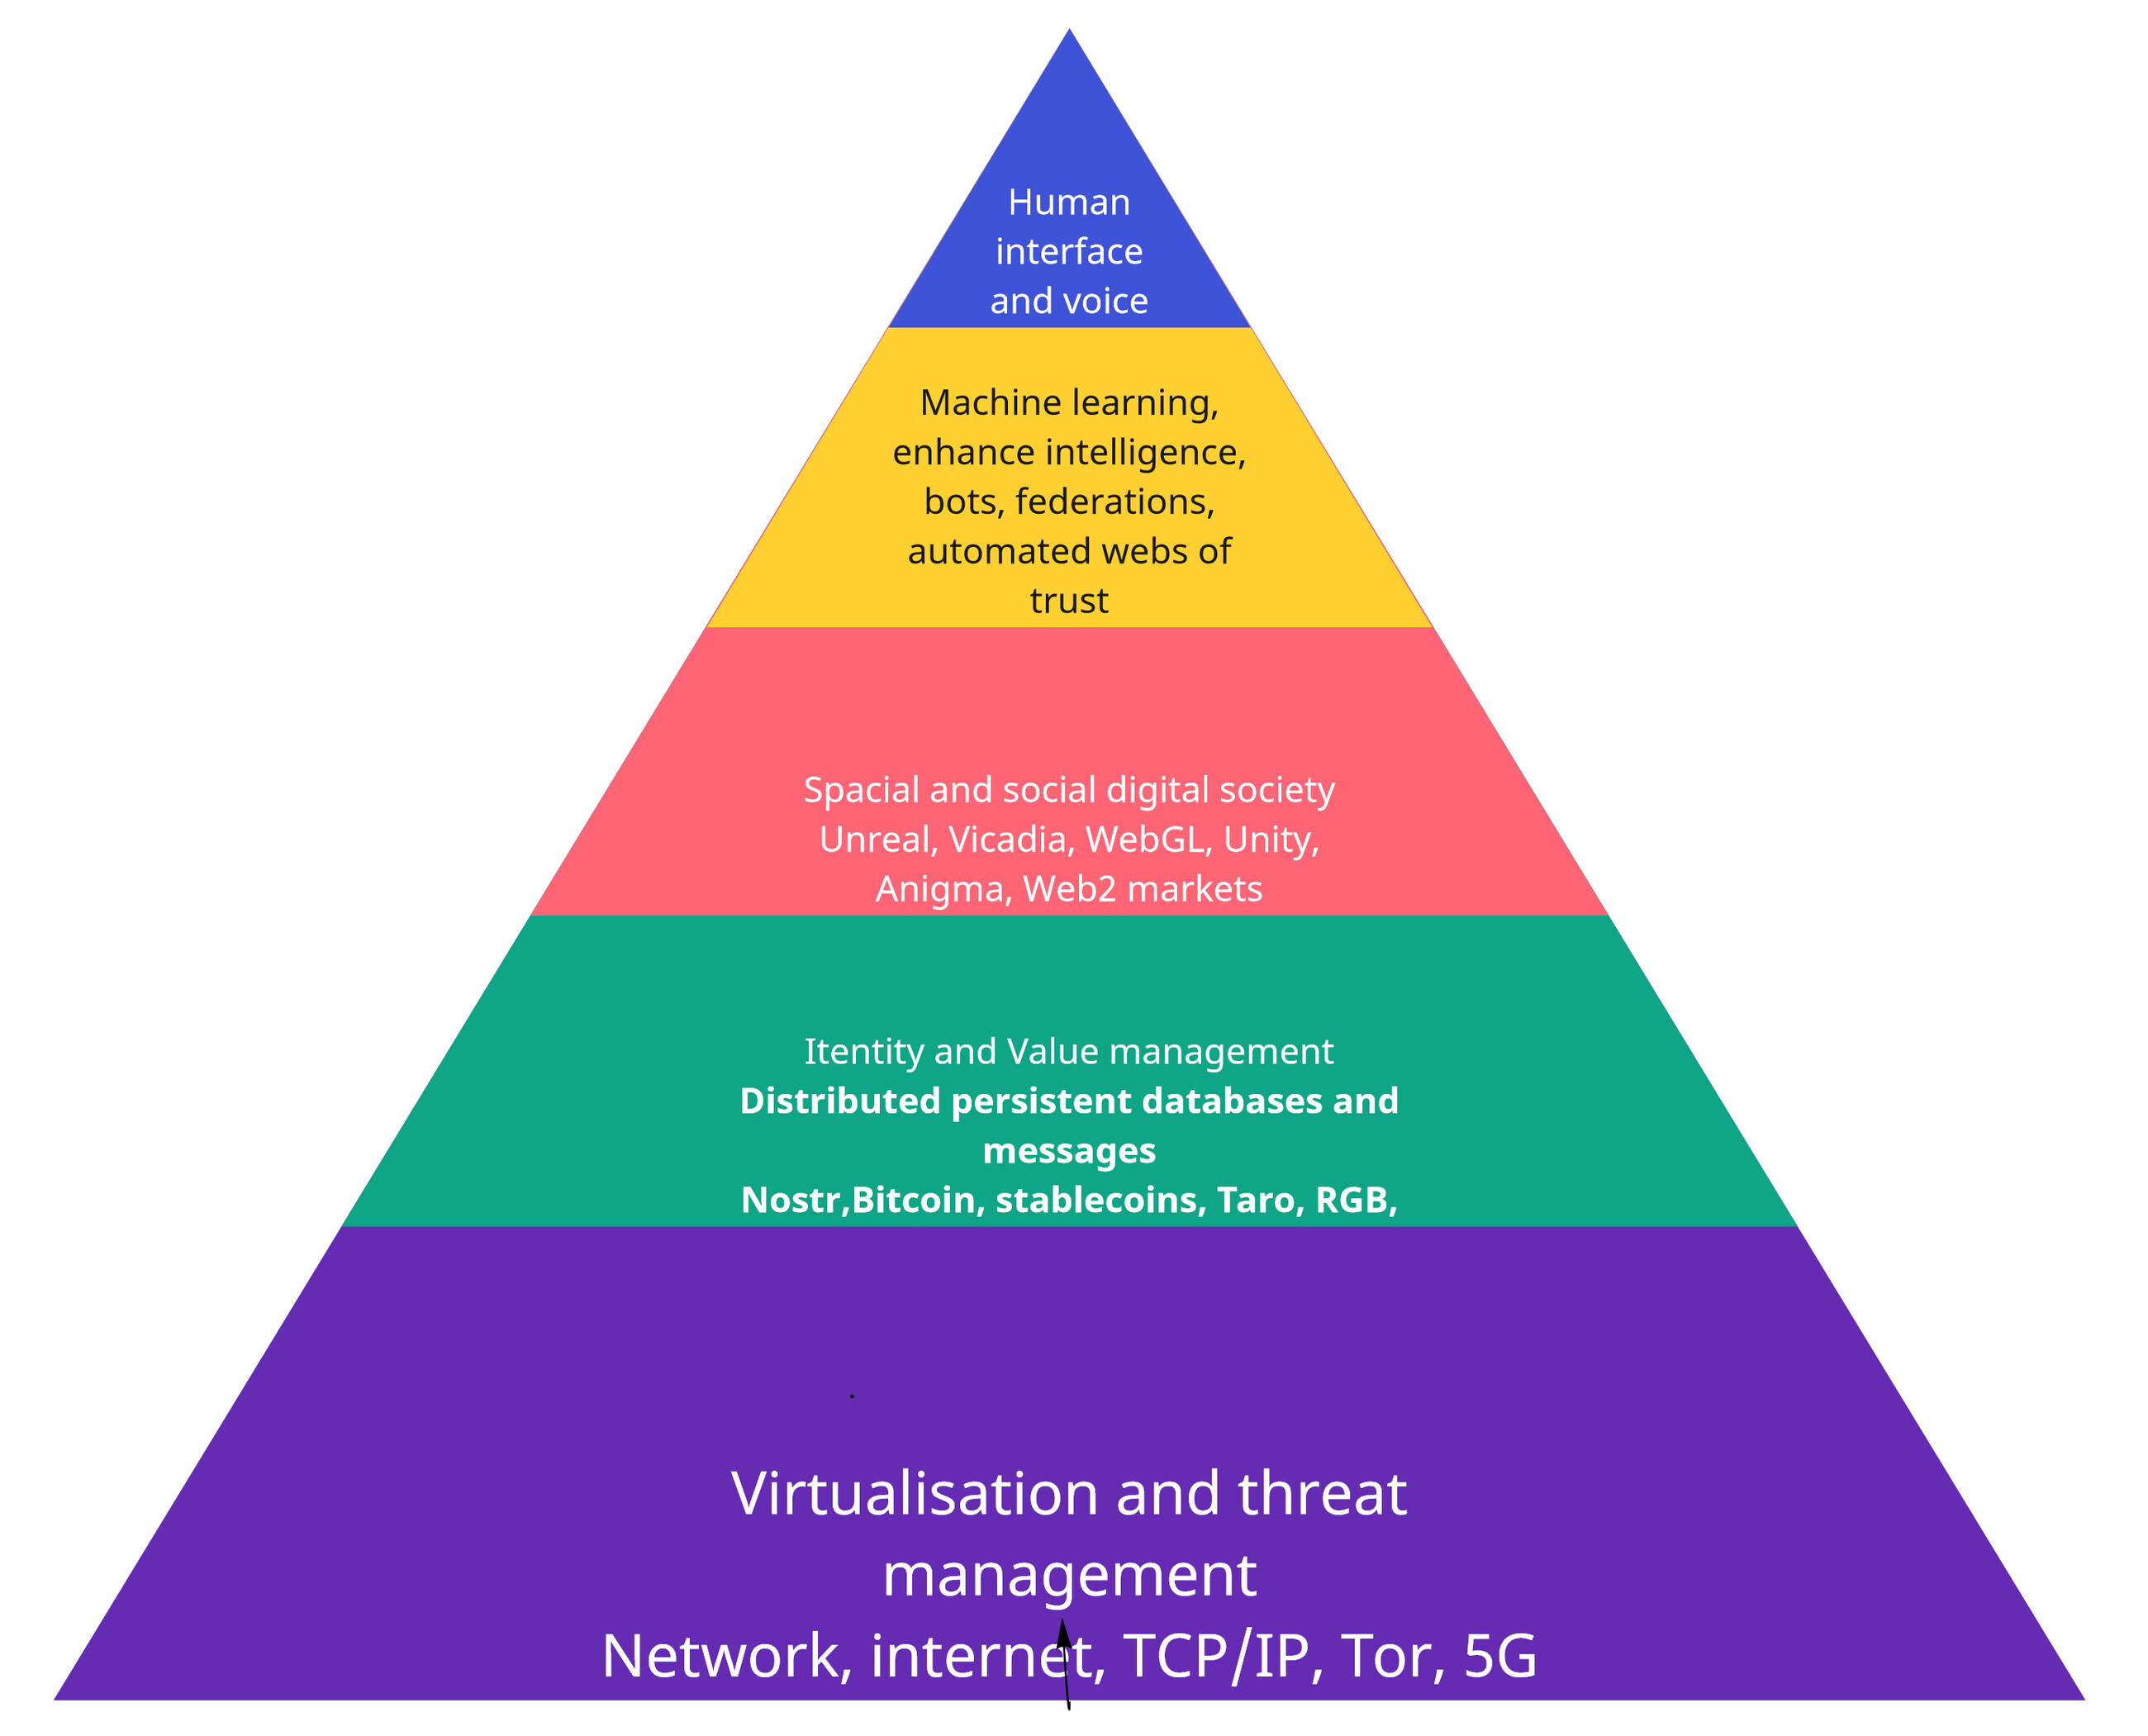
\includegraphics[width=0.8\textwidth]{b22-stack-pyramid.jpg}
\caption{The wager as printed: the 2022 book's layered stack --- network and Tor at the base, Bitcoin and Nostr as the identity and value layer, spatial engines above them, machine agents and webs of trust, and the human interface at the apex \parencite{OHare2022Convergence}. Reproduced exactly as published, original spellings included: a scored wager does not get its artwork retouched. Four years on, the ecosystem this book audits runs on the second layer and is still building the third and fourth.}
\label{fig:stack-pyramid}
\end{figure}

\begin{table}[ht]
\centering
\caption{Headline calls from \textit{Convergence and Disruption in Digital Society} (2022), graded against July 2026}
\label{tab:wager}
\begin{tabularx}{\textwidth}{L{4.6cm} X L{2.4cm}}
\toprule
\textbf{The 2022 call} & \textbf{The 2026 reckoning} & \textbf{Verdict} \\
\midrule
Vircadia's server architecture persists as the canonical metaverse model & Abandoned upstream; retired inside the author's own VisionFlow ecosystem & REFUTED \\
\addlinespace
Two billion people in the metaverse and a \$200\,bn virtual-goods market by 2026 & Metaverse hype collapsed; Meta itself dropped the branding & REFUTED \\
\addlinespace
Ordinals and RGB overtake Ethereum as the dominant NFT chain & The whole category shrank from its 2022 peak; RGB stayed niche & REFUTED \\
\addlinespace
Web5/ION wins a share of decentralised identity & Block shut it down in 2024; Nostr is the survivor & REFUTED \\
\addlinespace
2023 as the year of CBDC emergence & Digital euro and pound still unissued; the US banned domestic CBDC work & REFUTED \\
\addlinespace
A Bitcoin-and-Nostr DAO layer ends ``organisational mutexes'' & No traction; DAOs did not become mainstream governance & REFUTED \\
\addlinespace
Autonomous AI agents settle on Bitcoin rails & Right in direction; the market chose USDC-class rails (x402) & PARTLY \\
\addlinespace
White-collar automation at Goldman's 25 per cent scale & Direction right; the RLI's 2.5-to-16.1 per cent climb is still building toward it & PARTLY \\
\addlinespace
Most internet interactions synthetic within two decades ($\sim$2042) & Trending toward it on 2026 volumes; the deadline has not arrived & TOO-EARLY \\
\addlinespace
Real-estate savings deal office work its ``final blow'' by 2030 & The 2024--25 return-to-office reversals cut against it early & TOO-EARLY \\
\addlinespace
Meta-style corporate metaverse fails at audience capture; the opportunity is federated small-group collaboration & Horizons and Decentraland stagnated as predicted; the surviving practice is federated and small-group & CONFIRMED \\
\addlinespace
Nostr's web of trust beats classical DID/SSI standards & \texttt{did:nostr} is this ecosystem's production identity spine & CONFIRMED \\
\addlinespace
Sovereign states accumulate Bitcoin as a game-theoretic hedge & US Strategic Bitcoin Reserve; El Salvador and Bhutan continue & CONFIRMED \\
\addlinespace
Open-source LLMs reach GPT-4 parity by mid-2024 & Llama, DeepSeek, and Qwen met or beat the timeline & CONFIRMED \\
\addlinespace
Asynchronous coordination tooling becomes critical-path & Anticipates the 2026 escalation-over-approval finding & CONFIRMED \\
\bottomrule
\end{tabularx}
\end{table}

\section{Where the map held}

The hits cluster in one place: infrastructure the book expected to be built quietly and correctly, rather than launched loudly. The sharpest was identity. \textcite{OHare2022Convergence} bet against classical decentralised-identity and self-sovereign-identity standards and for Nostr's key-based web of trust, and that bet is now load-bearing in the author's own systems. \texttt{did:nostr} is the single production identity primitive across all six components of the VisionFlow ecosystem (Chapter~\ref{ch:visionflow-canon}), the exact choice the 2022 book argued for over Web5 and ION. The Bitcoin thread runs parallel. The claim that autonomous agents would need trustless settlement rails survives, in this ecosystem, as block-trails: Bitcoin-taproot-anchored, hash-chained provenance that lets an adversarial party verify an agent's audit record against the chain (Chapter~\ref{ch:visionflow-canon}). The market did not settle machine-to-machine payments on Bitcoin specifically, which is why the same prediction is graded a partial miss below; the anchoring instinct was right even where the currency call was not.

Three more held on their stated timelines. Open-source models reached GPT-4 parity close to the eighteen-month window the book named, as Llama, DeepSeek, and Qwen matched or beat it, which is arguably the sharpest technical call in the book. The Chinchilla-derived claim that data quality bound harder than parameter count became consensus the same year. The thread that connects the 2022 book most directly to this one is the telecollaboration thesis: the prediction, out of the author's two decades in human-scale mixed-reality telecollaboration, that asynchronous coordination tooling would become the critical-path technology for distributed teams. \textcite{Pereira2026Playbook} reports that in agentic workflows escalation beats approval by 71 to 30 per cent, the same asynchronous-over-synchronous logic the book named, arriving a chapter early and one substrate over.

Two smaller calls belong in the same column. The book predicted that Bitcoin mining would act as a grid-balancing load that withdraws when the grid needs peak power, and documented demand-response deployment on the Texas grid by 2025 bears that out. It also expected DAO-structured fundraising to keep drawing regulatory enforcement, which continued. Both are minor beside the identity and coordination threads, and both were right for the same reason those were: they described how a piece of infrastructure would behave under pressure, rather than how large a market would grow by a named year.

\section{Where it broke}

\begin{keyinsight}[title={A miss the author paid for personally}]
The cleanest way to trust a scorecard is to find the author's worst call and check that it is graded honestly. Here it is. The book bet its own deployment chapters on Vircadia's domain and metaverse-server architecture persisting as the canonical model for shared worlds. Vircadia was abandoned upstream, and the presence bridge built on that model inside VisionClaw now sits in the codebase disconnected by default, recorded in Chapter~\ref{ch:gap-register} as an avatar renderer and Vircadia bridge that exist as code but are never instantiated. The platform the book backed died under the system the author later built on it. That is platform risk stated from the inside.
\end{keyinsight}

The metaverse forecast is the book's single cleanest falsification, and it splits in a way the scorecard should preserve. The headline numbers, two billion people in the metaverse by 2026 and a \$200\,bn virtual-goods market, were industry forecasts the book carried from McCann Worldgroup and its peers; they collapsed hard enough that Meta itself quietly dropped the branding. The book's own analysis, written from decades of laboratory telecollaboration, bet the other way: it held that large-scale social virtual reality was underperforming ordinary video calls, that the value lay in federated small-group collaboration rather than spectacle, and it named Horizons and Decentraland as continuing failures in audience capture. The reported forecasts were refuted; the authors' contrarian read of them was confirmed. Carrying a forecast you disbelieve is still a form of endorsement, so the refuted rows stand in the table, but the split matters for calibration: the misses concentrate where the book deferred to the era's consensus, and thin out where it argued from its own laboratory evidence.

The NFT chapter aged badly with no such split: the bet that Bitcoin-native Ordinals and RGB would overtake Ethereum lost twice over, because the whole category shrank from its 2022 peak and Ethereum kept the diminished remainder. An authorship note belongs here, stated the way the lead author states it: the NFT chapter was a co-author's, and the lead author's scepticism of the category predates the collapse. The wager stands regardless. A book signed by three names is a bet by all three, and the score is recorded as printed rather than reallocated in hindsight. Two monetary predictions reversed outright rather than merely running late. The book had 2023 as the year of central-bank digital-currency emergence; by 2026 the digital euro and the digital pound remain unissued and the United States has banned domestic CBDC development. It expected a proposed 30 per cent US mining tax to gut domestic mining; the tax never passed and 2025 turned pro-mining instead, into executive orders and a Strategic Bitcoin Reserve, which is the opposite of the forecast direction.

One miss is the exact mirror of one of the hits. The book hedged its identity bet across Nostr and Jack Dorsey's Web5/ION; Block shut Web5 down in 2024, and the surviving half of that hedge is the half this ecosystem runs on. The DAO chapter proposed a Bitcoin-and-Nostr coordination layer, ``Stackerstan'', that would dissolve what it called organisational mutexes through votepower and asynchronous problem-claiming. It never gained traction, and DAOs did not become the governance substrate the book expected. The mechanism failed. What it was built to solve outlived it, and the next section is where that matters.

\section{Partial credit}

Between the clean hits and the clean misses sit the calls that were right in direction and wrong in detail, and the honesty ethic requires scoring the detail. The agent-settlement prediction is the sharpest of these. The book was right that autonomous agents would need trustless settlement rails, and wrong about the instrument: the 2026 agent-commerce market gravitated to USDC-class stablecoins and protocols such as x402, not to Bitcoin. The author's own ecosystem, anchoring provenance to Bitcoin through block-trails, is the exception that proves the market rule rather than a refutation of it. Two more sit alongside. The claim that Ethereum's move to proof-of-stake would concentrate control in a handful of entities is directionally right, given staking concentration around Lido and the large exchanges, and overstated how politically salient that concentration would become. And the white-collar-automation forecast, pitched at Goldman's 25 per cent displacement figure, has the direction right while the scale is still building toward it: the Remote Labor Index's climb from 2.5 to 16.1 per cent in eight months is consistent with the trajectory without yet reaching the number.

\section{What 2022 could not see}

Two of the most consequential features of the 2026 landscape are absent from a 515-page book written to anticipate it. The first is the subject of this book. Stackerstan tried to remove organisational mutexes with blockchain votepower and failed; four years later the multi-agent literature documents the identical structural problem in a new substrate, where coordination without a hierarchy substitute breaks under load. \textcite{Cemri2025} measures failure rates of 41 to 86.7 per cent across seven state-of-the-art frameworks. The 2022 book wrote a chapter about coordinating autonomous parties without a manager and never connected it forward to what would become the defining failure mode of agentic systems. It described the problem in one costume and did not recognise it in the next.

The second blind spot is more personal, and this book will not dress it up. The 2022 book theorised AI as an economic actor and imagined agents holding wallets and settling payments. Nothing in it anticipated that the author, a non-programmer, would use agentic AI collaboration to build a roughly 600,000-line, six-repository production ecosystem in eighteen months: the same ecosystem this book audits. The book saw AI as a party to the economy. It missed AI as a coding collaborator that erases the line between the programmer and the person who cannot program, which is the precondition for everything in Part~\ref{part:visionflow}.

A third gap is narrower but sharp. The book's strongest technical instinct, that data quality rather than parameter count was the binding constraint on model capability, was right, and it became industry consensus by 2024. It had no model for what came next: inference-time reasoning compute, the chain-of-thought reinforcement learning of the 2024--25 frontier, an axis orthogonal to both parameters and training data. Getting the last constraint right buys no view of the next one.

\section{The through line}

Read the hits and misses together and a single design decision falls out of them. The 2022 book's metaverse scepticism was not a mood; it was the conclusion of a research programme that had spent two decades measuring why virtual environments failed to gain traction. The diagnosis it reached was that the blocker was never rendering or immersion. It was the substrate underneath: no verifiable identity, no sovereign shared data, no native way to move value, and communication channels that discarded the gaze, spatiality, and turn-taking cues that trust rides on. The book named three jointly unsolved problems --- value transmission without gatekeepers, provable distributed identity for mixed reality, and generative-AI access for the excluded --- and those three problems are, one for one, the pillars of the ecosystem in Part~\ref{part:visionflow}: the 402 web-ledger with its block-trails, the \texttt{did:nostr} spine, and an agent mesh built for roughly four thousand pounds.

VisionFlow is therefore not a metaverse play that kept the faith through the collapse. It is the autopsy, acted on: substrate first, embodiment second. That ordering also reframes the sharpest finding in Chapter~\ref{ch:gap-register}. The register found that the mesh acts and mostly cannot yet be seen acting --- the governance and identity layers run ahead of the visible surfaces. Read against the 2022 diagnosis, that asymmetry is the signature of a four-year-old sequencing decision rather than an oversight: the visible layer was never the blocker, so it was deliberately built last. The gap is real and scheduled (Chapter~\ref{ch:ecosystem-roadmap}); what the lineage adds is the documented reason the schedule runs in that order.

\section{Calibration for what comes next}

Add the columns up and the pattern does not flatter in the usual way. The book's confident, headline-grabbing calls, the metaverse at scale, CBDCs imminent, DAOs as governance, Bitcoin NFTs winning, are where it was most wrong. Its quiet infrastructure calls held: Nostr over classical identity standards, Bitcoin as a sovereign hedge, open-source model parity, data quality over scale, and asynchronous coordination becoming the thing that matters. The hits are the plumbing; the misses are the marketing.

That is what the scorecard is for. It calibrates this book's forward claims rather than conferring authority on them by seniority. When Chapter~\ref{ch:ecosystem-roadmap} commits, in print, to measurable compounding in the DreamLab ecosystem within two quarters, a reader is entitled to price in the author's demonstrated failure rate on four-year horizons, and to discount the confident register more steeply than the quiet one. The falsifiable-predictions ethic this book asks of itself in Chapter~\ref{ch:gap-register} and Chapter~\ref{ch:open-questions} is a habit with receipts, run once already and scored here rather than buried.

\begin{cautionbox}[title={How to read this book's forward claims}]
Trust the infrastructure register, discount the headline register. The 2022 calls that held were quiet and structural; the calls that failed were confident and dated to a year. Where this book makes a confident, dated forward claim, weigh it against that pattern before acting on it. A book that grades its author's last set of public bets, and grades the misses first, is asking to be read at a discount it has itself calculated.
\end{cautionbox}

\chapter{Open Questions and Research Directions}
\label{ch:open-questions}

\epigraph{A working document that hides its weaknesses is less useful than one that maps them. These gaps are research directions, not admissions of failure.}{}

This chapter is an exercise in intellectual honesty. The coordination collapse thesis, as presented in this report, is incomplete. The evidence base has specific weaknesses. The analysis contains blind spots visible to each of its three audiences. Several important topics are missing entirely. Mapping these gaps is not an admission of failure. It is a research agenda.

\section{The Core Thesis Is Incomplete}

The report frames hierarchy as an information routing protocol and argues that AI collapses the cost of that routing to near-zero. This framing is analytically productive: it generates the coordination collapse concept, the judgment broker role, and the compounding organisation model. But hierarchy performs at least five functions, of which information routing is only one.

\subsection{Legitimation}

Who has authority to commit resources? The mesh can route information and even recommend resource allocation, but it cannot \emph{authorise} a \pounds 2 million capital expenditure. Legitimation (the organisational mechanism by which decisions acquire binding authority) is a function of hierarchy that AI does not replace. A judgment broker who validates a shadow workflow is exercising legitimate authority derived from their position in the organisational structure. Remove the structure, and the authority evaporates.

\subsection{Accountability}

Who is fired when things go wrong? ``The mesh decided'' is not an answer a board of directors accepts. Accountability requires identifiable humans who bear consequences for outcomes. The judgment broker role addresses this partially (the broker who validates a workflow bears accountability for that validation), but the full accountability architecture for agentic systems is not worked out. When an agent in the mesh makes a decision that produces a regulatory violation, the chain of accountability must be traceable to a human. The declarative governance layer (Chapter~\ref{ch:governance}) provides audit trails, but audit trails are not the same as accountability structures.

\subsection{Political Negotiation}

Whose priorities win when budgets are finite? AI can optimise within constraints; it cannot set the constraints. The allocation of scarce resources across competing priorities is fundamentally a political act: a negotiation among stakeholders with different interests, values, and power. The mesh can surface information that makes the negotiation more transparent, but it cannot replace the negotiation itself.

\begin{cautionbox}[title={An Honest Reframing}]
If three of hierarchy's five core functions persist (legitimation, accountability, and political negotiation), then ``coordination collapse'' may be an overstatement. A more honest framing: \textbf{information routing collapse} --- one function of hierarchy dissolves, forcing the others to restructure around different assumptions. The coordination tax shrinks dramatically; it does not reach zero. This report uses the more provocative framing because it captures the magnitude of the disruption, but the qualification belongs in the analysis.
\end{cautionbox}

\textbf{Research needed}: How do legitimation, accountability, and political negotiation operate in post-hierarchical structures? Haier's micro-enterprise model provides the best existing evidence but operates in a culturally specific context that may not generalise.

\section{Evidence Base Weaknesses}

The argument in this report rests on specific empirical findings. Several of these findings have limitations that deserve explicit acknowledgement.

\subsection{The Jagged Frontier Map Is Outdated}

The BCG experiment \parencite{DellAcqua2026} used GPT-4 (now two model generations behind current frontier models). The specific task boundaries identified in that study --- the 18 tasks inside the frontier and the business judgment task outside it --- have almost certainly shifted. Models released since the study likely perform well on tasks that were outside GPT-4's frontier.

This does not invalidate the concept. The jagged frontier is a structural feature of AI capability, not a fixed map. The principle (that adjacent tasks can fall on opposite sides of the boundary, and that the boundary is unpredictable) holds regardless of where the boundary currently sits. But any practitioner using this report to make operational decisions must retest the frontier with current models in their specific domain. The 2023 map is a historical reference, not a current navigation chart.

The concern is now partially answered by continuous measurement rather than a fixed retest. The Remote Labor Index \parencite{RLI2025, CAIS2026RLI} provides exactly the longitudinal, client-quality re-measurement this section called for: automation of real freelance deliverables (judged against a paying-client bar, not a benchmark proxy) rose from 2.5 to 16.1 per cent in eight months. That trajectory confirms both halves of the jagged frontier claim simultaneously: the frontier is still jagged (professional-quality performance still fails on the large majority of projects) and it is moving fast (the boundary shifted 6.4-fold in under a year). The residual gap is real, though: the RLI measures freelance deliverables, not the coordination tasks inside an organisation that this report is actually about. A practitioner still has to map their own domain's frontier. The RLI tells them how urgently, not where.

\subsection{The 17$\times$ Error Source: Resolved}

The first edition of this report leaned on a 17-times error multiplication statistic \parencite{TDS2026} to ground the case against naive multi-agent deployment, support the judgment broker role, and supply the quantitative punch behind the ant death spiral narrative. The source was Towards Data Science --- a community-edited blogging platform, not a peer-reviewed journal. This chapter flagged it as the report's weakest load-bearing number. The literature has since delivered a replacement.

\textcite{Cemri2025}, published at NeurIPS 2025 (Datasets and Benchmarks Track) and therefore peer-reviewed, documents failure rates of 41 to 86.7 per cent across seven state-of-the-art open-source multi-agent frameworks (ChatDev, MetaGPT, HyperAgent, AppWorld, AG2, Magentic-One, and OpenManus), drawn from more than 1,600 annotated execution traces with inter-annotator agreement of Cohen's $\kappa = 0.88$. The paper does more than replace a number: it supplies a causal taxonomy of fourteen failure modes across three categories (specification issues, inter-agent misalignment, and task verification), so the error-multiplication argument now rests on a documented mechanism rather than an unexplained multiplier. \parencite{Khanal2026} adds an independent second line of evidence: across 23,392 episodes, frontier models show the \emph{highest} long-horizon meltdown rates, up to 19 per cent, precisely because their capacity for ambitious multi-step strategies is what lets them spiral further before failing. Memory scaffolds, the intuitive fix, universally hurt long-horizon performance across every model tested.

\begin{cautionbox}[title={What Changed}]
The phenomenon the 17$\times$ figure gestured at (error propagation and amplification in multi-agent chains) was always real. What was weak was the citation, not the claim. \parencite{Cemri2025} and \parencite{Khanal2026} now give that claim a peer-reviewed evidence base, a causal taxonomy, and a falsification of the ``more memory fixes it'' intuition. The 17$\times$ figure is retired from this edition and survives only as the superseded early estimate it always was.
\end{cautionbox}

\subsection{The Klarna Narrative Is Cherry-Picked}

Klarna's 2025 financials showed improved margins alongside the customer satisfaction decline described in Chapter~\ref{ch:three-models}. The CEO's admission that ``cost unfortunately seems to have been a too predominant evaluation factor'' \parencite{Klarna2025} comes from a longer statement that also defended the AI strategy as a necessary evolution. Presenting only the quality degradation without the financial improvement is selective evidence: the kind of rhetorical move that a hostile reader will identify and use to dismiss the broader argument.

The honest presentation: Klarna achieved short-term cost reduction, experienced quality degradation, began rehiring humans, and the CEO acknowledged the trade-off. The lesson is not ``AI customer service fails'' but ``optimising for cost alone, without maintaining human oversight at quality-sensitive boundaries, produces predictable quality collapse.'' This is a more nuanced and more defensible claim.

The July 2026 picture sharpens this lesson rather than complicating it. Klarna's current operating model is not a simple reversal to the pre-2023 staffing level but an explicit AI-plus-human hybrid \parencite{KlarnaHybrid2026}: AI continues to handle high-volume routine queries, while human staff (hired on flexible, gig-style contracts rather than reinstated as the original full-time roles) are reserved for the empathy, discretion, and escalation cases the CEO's own admission identified as under-served. This is not evidence against AI customer service; it is evidence against one specific configuration of it. The stable end state is neither ``all AI'' nor ``all human'' but a designed division of labour at the jagged frontier --- the judgment-broker architecture this report proposes, arrived at independently by a company that started from the opposite assumption.

\subsection{The 89 Per Cent Reduction}

The claim that providing approved AI tools reduces unauthorised use by 89 per cent is used repeatedly in this report. No primary source is cited. The statistic is plausible (it aligns with shadow IT research showing that sanctioned alternatives reduce unsanctioned adoption), but a claim used this frequently requires a traceable citation. This is an open research gap.

\subsection{Vendor Report Methodology}

The shadow AI statistics used throughout the report stack vendor-funded research (Gartner, IBM, Capgemini) that has methodological limitations and commercial incentives to inflate threat numbers. No error bars, confidence intervals, or methodological caveats are provided. A reader from an academic background will note this immediately. The statistics should be treated as directionally correct rather than precisely accurate.

\section{Audience Blind Spots}

\subsection{No Day-in-the-Life}

Middle managers will ask: ``What does my Monday morning look like as a judgment broker? What am I literally doing at 9am?'' This report offers the conductor metaphor, the role transformation table, the three irreplaceable capacities --- yet it provides no concrete job specification, no competency framework, no salary benchmarking, no day-in-the-life narrative. The abstraction is intellectually satisfying but operationally insufficient for a middle manager trying to decide whether to invest in this transition.

\textbf{Research direction}: develop detailed judgment broker role specifications for three to five industry verticals, including day-in-the-life scenarios, competency models, and compensation benchmarking.

\subsection{No Total Cost of Ownership}

AI leaders will ask: ``What does this cost for a 500-person organisation? What is the ROI timeline?'' Chapter~\ref{ch:implementation} provides an indicative cost tier model, but this falls short of a total cost of ownership analysis that includes ongoing compute, model API costs (which are volatile and trending downward), knowledge engineering maintenance, judgment broker training, and the opportunity cost of the transition period. Without financial modelling, the implementation roadmap is a strategic argument, not a business case.

\textbf{Research direction}: develop a TCO calculator parameterised by organisation size, industry vertical, regulatory burden, and existing technology infrastructure.

\subsection{The Roadmap Contradiction}

Change managers will notice that this report attacks Kotter and ADKAR for being phased transformation models, then offers a phased 90-day roadmap. Chapter~\ref{ch:change-problem} addresses this contradiction explicitly (framing the roadmap as a bootstrap sequence rather than a change plan), but the resolution requires the reader to accept a distinction that may feel like sophistry. The tension is genuine and deserves continued intellectual engagement rather than a single paragraph of resolution.

\subsection{The Analyst-Vendor Conflict}

All three audiences will notice that DreamLab AI Consulting is simultaneously the analyst (producing this report), the framework creator (proposing the Dynamic Agentic Mesh), and the vendor (operating VisionClaw). This is a classic consulting positioning conflict. The report's credibility depends on acknowledging this conflict directly: ``We built this because we believe it. Here is the evidence for and against. Judge the framework on its merits, not its provenance.''

\section{Engaging with Acemoglu}

Daron Acemoglu's work on AI and productivity has been cited in this report's bibliography but not substantively engaged with in the main text. This is a significant omission because Acemoglu's thesis directly challenges the optimistic productivity assumptions underlying the coordination collapse argument.

\begin{evidencebox}[title={The Acemoglu Sceptical Thesis}]
In ``The Simple Macroeconomics of AI'' \parencite{Acemoglu2025}, Acemoglu argues that AI's impact on total factor productivity (TFP) will be modest (at most \textbf{0.66 per cent over 10 years}. His reasoning:

\begin{enumerate}
  \item AI automates tasks, not jobs. The tasks most amenable to automation are not necessarily the tasks that contribute most to productivity.
  \item The ``easy-to-learn, hard-to-verify'' problem: many tasks that AI can perform require costly human verification, limiting net productivity gains. This maps directly onto the vigilance problem described in Chapter~\ref{ch:vigilance}.
  \item New task creation (historically the mechanism by which automation generates employment growth) may be slower with AI than with previous technologies.
  \item AI may increase inequality rather than aggregate productivity, concentrating gains among capital owners and high-skill workers while displacing middle-skill employment.
\end{enumerate}
\end{evidencebox}

The coordination collapse thesis should engage with Acemoglu on three fronts.

\textbf{First}, the 0.66 per cent TFP estimate applies to the economy as a whole, not to individual organisations. An organisation that deploys an agentic mesh effectively may capture disproportionate productivity gains precisely because its competitors do not. The compounding organisation thesis does not require AI to transform the macroeconomy; it requires AI to provide a competitive advantage to organisations that use it well. This is consistent with Acemoglu's framework: the gains are real but unevenly distributed.

\textbf{Second}, the task-level analysis is compatible with the jagged frontier concept. Acemoglu's point that AI automates tasks, not jobs, aligns with the argument that the judgment broker's role is to determine which tasks sit inside the frontier and which require human judgment. The mesh architecture is explicitly designed around task decomposition, not wholesale job replacement. Where Acemoglu warns that the ``easy-to-learn, hard-to-verify'' problem limits productivity gains, the mesh responds with HITL Precision and Trust Variance monitoring (architectural mechanisms for managing verification costs).

\textbf{Third}, the equity concern is serious and currently unaddressed in this report. If the mesh concentrates productivity gains among organisations with the capital and technical expertise to deploy it, while displacing middle-skill workers in organisations that cannot, the net social effect may be increased inequality even as individual organisations benefit. This is a genuine tension that the coordination collapse thesis does not resolve.

\textbf{Fourth}, the RLI trajectory \parencite{RLI2025, CAIS2026RLI} puts pressure on Acemoglu's implicit pace assumption without threatening his mechanism. An automation rate that moved from 2.5 to 16.1 per cent of client-quality freelance deliverables in eight months is a fast-moving frontier by any standard; if that pace continued, the case for a durable 0.66 per cent TFP ceiling would look increasingly strained. But 16.1 per cent automation of freelance deliverables is entirely compatible with modest aggregate productivity gains if verification and integration costs dominate. Acemoglu's ``easy-to-learn, hard-to-verify'' problem, restated at the level of task completion rather than macroeconomic output, maps directly onto this constraint. \textcite{Liu2026} now gives that mechanism a formal home: contextual transaction cost includes an explicit verification-burden term, and the finding that collective efficiency collapses 91.4 per cent from the lowest to the highest CTC quartile is, in effect, a microfoundation for why task-level automation does not translate one-for-one into organisational or macroeconomic productivity (Chapter~\ref{ch:coordination-economics}).

\textbf{Fifth}, the firm-level evidence assembled since April supports both halves of this report's reading, and Acemoglu's distributional concern besides. \textcite{RampRevelio2026} and the Box survey reported by \textcite{Levie2026} (the latter resting on a single social-media source without published methodology) show real gains at the firm level, but gains concentrated among organisations that have already adopted AI intensively, with high-intensity adopters growing headcount 10.2 per cent over two years while low-intensity adopters showed no significant change. That is uneven distribution \emph{across} organisations, exactly as this report's compounding-organisation argument predicts. \parencite{Brynjolfsson2025Canaries} supplies the complementary, and more troubling, half: uneven distribution \emph{within} the labour market, with early-career workers in AI-exposed occupations showing a roughly 16 per cent relative employment decline since late 2022. Acemoglu's equity concern was speculative in the first edition of this report. It is now measured.

\section{New Open Questions (July 2026)}

The evidence that arrived since April resolves several of this chapter's original flags. It also opens new ones. Five deserve explicit tracking.

\begin{itemize}
  \item \textbf{CTC measurement in production.} \textcite{Liu2026} gives contextual transaction cost a rigorous definition and shows it predicts collective efficiency in simulation and in trace-instrumented real-LLM runs. The instrumentation is no longer absent: AgentBox now runs a contextual-transaction-cost emitter on its hook spine, forwarding a per-workflow token-count-and-handoff envelope, above a native context-compression layer (\texttt{headroom-napi}/CCR) whose audit trail is barred by hard-coded rule from ever being compressed (Chapter~\ref{ch:agentbox}). What genuinely remains open is comparability, not existence: no agreed unit or method yet lets one mesh's CTC be read against another's, and the first production figure from that emitter is still to be reported (Recommendation~3 of Chapter~\ref{ch:ecosystem-roadmap}). The KPIs proposed in Chapter~\ref{ch:new-kpis} now have both a theoretical anchor and a running meter; what they lack is a cross-mesh baseline against which a given reading counts as good or bad.
  \item \textbf{The broker-apprenticeship problem.} If entry-level roles in AI-exposed occupations decline \parencite{Brynjolfsson2025Canaries} while adopting firms hire AI-fluent juniors rather than training them from scratch \parencite{RampRevelio2026}, where does the next generation of judgment brokers learn the domain expertise the role requires? The answer plausibly differs for adopting and non-adopting firms, which would make broker scarcity a compounding advantage for early movers. This is a mechanism this report has not modelled.
  \item \textbf{The design question is contested.} \textcite{Dochkina2026} reports self-organising agent collectives, with autonomous role selection, outperforming both fully centralised coordination and fully designed structures. This contrasts with the finding of \textcite{Liu2026} that adaptive, CTC-aware orchestration beats unstructured collectives. Both are single studies with different task distributions and scales. The field has not converged on whether agent collectives should be designed, allowed to self-organise, or some specific hybrid of the two, and this report should not pretend otherwise.
  \item \textbf{Survivor bias in the deployment evidence.} \textcite{Pereira2026Playbook} study the successful 5 per cent of deployments against the baseline of \textcite{MITNANDA2025}, in which most pilots produced no measurable P\&L impact. That comparison is valuable for identifying what successful deployments have in common, but it cannot answer how common success is, because the sample is selected on the outcome. Prevalence estimates should not be derived from playbook-style evidence, however good the playbook.
  \item \textbf{The RLI-to-jobs mapping.} The Remote Labor Index measures automation at the level of individual, client-quality deliverables. No method yet exists to translate a deliverable-level automation rate into an occupation-level displacement forecast. The tasks-versus-jobs distinction that \textcite{Chatterji2026} raises applies with full force to the RLI's own headline number. Sixteen per cent of freelance deliverables being automatable at professional quality is not the same claim as sixteen per cent of any job disappearing, and this report has not built the bridge between the two.
\end{itemize}

\section{Energy and Environmental Costs}

The report proposes deploying agentic infrastructure at organisational scale without addressing the energy implications. This is an increasingly visible omission as the environmental costs of AI infrastructure become a matter of public and regulatory concern.

\begin{evidencebox}[title={The Energy Cost of Agentic Systems}]
\begin{itemize}
  \item \textcite{Patterson2025} at Microsoft Research find that reasoning-intensive queries (the kind that agentic orchestration relies on) have a median energy cost of 4.32 Wh per query, compared to 0.34 Wh for standard queries. This represents a \textbf{43$\times$ increase} in energy consumption for the reasoning-heavy workloads that an agentic mesh generates continuously.
  \item \textcite{NatureSustainability2025} projects that US AI server infrastructure will produce \textbf{24--44 Mt CO$_2$-equivalent annually} through 2030. This range is growing as model sizes increase and inference demand scales.
  \item An agentic mesh running continuous orchestration, discovery monitoring, and governance checks generates substantially more inference load than on-demand AI tool use. The compound flywheel, by design, \emph{increases} inference volume as the mesh becomes more active.
\end{itemize}
\end{evidencebox}

The energy cost of the mesh is not merely a corporate social responsibility issue. It is a business cost that scales with mesh activity. Organisations deploying agentic infrastructure must account for compute costs that are qualitatively different from traditional IT expenditure: costs that increase as the mesh becomes more capable, not less.

\textbf{Research direction}: develop energy cost models for agentic mesh deployment at different organisational scales, including comparison with the energy cost of the human coordination infrastructure the mesh replaces (office buildings, commuting, business travel). The net energy equation is not obviously negative --- a 200-person management layer has its own carbon footprint --- and it is not obviously positive.

\section{Cybersecurity Attack Surface}

The statistic that financial services organisations manage 96 machine identities per human \parencite{CyberArk2025} (with only 31 per cent having controls in place) is cited in Chapter~\ref{ch:industry-landscape} as a governance issue. It is also a security issue that the report does not adequately address. An agentic mesh creates a dramatically expanded attack surface:

\begin{itemize}
  \item Each agent skill is a potential vector for prompt injection: an adversary who can manipulate an agent's input can redirect its behaviour within its authority boundary.
  \item The OWL~2 ontology that provides shared semantics is a single point of corruption: poisoning the ontology could redirect agent routing across the entire mesh.
  \item The Nostr identity layer provides cryptographic verification but depends on key management practices that most organisations have not developed for non-human identities.
  \item The Insight Ingestion Loop creates a pathway from frontline input to production workflows: a supply chain vulnerability that adversaries could exploit by planting malicious ``shadow workflows.''
\end{itemize}

\textbf{Research direction}: systematic threat modelling for agentic mesh architectures, including adversarial analysis of the Insight Ingestion Loop and ontology poisoning scenarios.

\section{Equity and Access}

Who benefits from the mesh and who is structurally excluded? The report addresses middle managers (a specific professional cohort) but does not address:

\begin{itemize}
  \item Workers without AI literacy who cannot participate in the discovery layer.
  \item Roles that do not lend themselves to agent augmentation: physical labour, care work, creative work that resists decomposition into tasks.
  \item Organisations in the Global South that lack the infrastructure and capital to deploy agentic systems.
  \item The distributional effects within organisations: does the mesh flatten compensation as it flattens hierarchy, or does it concentrate value in the judgment broker tier?
\end{itemize}

Acemoglu's concern about AI increasing inequality rather than productivity is most acute here. If the Dynamic Agentic Mesh is a tool available primarily to well-capitalised organisations in knowledge-intensive industries, its net effect may be to widen the gap between those organisations and everyone else. This is a dynamic that the \textcite{WEF2025} Future of Jobs Report anticipates when it projects 170 million new roles created alongside 92 million displaced.

\section{Competing Frameworks Not Addressed}

The report positions against Block and Every. Neither is a consulting framework the target audience is actively evaluating. It does not differentiate substantively from:

\begin{itemize}
  \item \textbf{SAFe 6.0} \parencite{SAFe2024}, which added AI-specific agile change patterns in 2024.
  \item \textbf{Microsoft Copilot Studio} \parencite{MicrosoftCopilotStudio2025}, an enterprise organisational AI deployment framework with the largest existing footprint.
  \item \textbf{Holacracy 5.0} \parencite{Holacracy2024}, which specifically addressed the scale failures attributed to earlier versions.
  \item \textbf{Anthropic's constitutional AI governance}, directly relevant to the governance paradox in Chapter~\ref{ch:governance}.
\end{itemize}

A competitor comparison table is provided in Appendix~\ref{ch:competitor-matrix}, but the main text does not engage with these alternatives at the depth they deserve.

\section{The VisionClaw Credibility Gap}

Chapter~\ref{ch:technical-substrate} describes VisionClaw honestly, including both its genuine capabilities and its limitations. But the credibility gap between a 15-person creative technology team and a 500-person manufacturing firm has not been bridged. The favourable conditions under which VisionClaw operates (high technical literacy, low process rigidity, flat power dynamics, intrinsic motivation, the system architect as the primary user) are the most favourable possible environment.

\begin{keyinsight}
VisionClaw is an existence proof under ideal conditions, not a proof of general applicability. The coordination collapse thesis requires bridging evidence that the architecture works in less favourable environments: regulated industries, non-technical workforces, unionised labour, legacy ERP systems, and middle managers who did not choose the system.

Four bridging strategies are available:
\begin{enumerate}
  \item Run a pilot in a genuinely different context (regulated industry, non-technical workforce).
  \item Partner with an established consulting framework (Deloitte, BCG) for independent validation.
  \item Publish the methodology as open-source and invite external testing.
  \item Position VisionClaw explicitly as ``existence proof under favourable conditions'' and build the evidence base incrementally.
\end{enumerate}
The fourth strategy is the one this report adopts. The others represent the research agenda.
\end{keyinsight}

\section{Additional Failure Modes}

The report documents two failure modes in detail: the ant death spiral (agents responding to agents in infinite loops) and the vigilance degradation problem (humans falling asleep at the wheel as AI quality improves). But an agentic mesh at organisational scale introduces additional failure modes that this analysis does not adequately address:

\begin{itemize}
  \item \textbf{Cascading errors}: a single incorrect agent output propagating through downstream agents before the judgment broker can intervene.
  \item \textbf{Single point of failure in the judgment broker}: if the broker is unavailable, incapacitated, or overwhelmed, the mesh has no fallback governance mechanism.
  \item \textbf{Ontology drift}: the OWL~2 ontology gradually diverging from the actual business domain as the organisation evolves, producing increasingly inaccurate agent routing.
  \item \textbf{Metric gaming}: agents optimising for the four KPIs in ways that satisfy the metrics while degrading actual performance. This is Goodhart's law applied to agentic governance.
  \item \textbf{Cultural rejection}: the mesh may function technically while being socially rejected by the workforce, producing compliance without engagement.
\end{itemize}

\textbf{Research direction}: systematic failure mode analysis (FMEA) for agentic mesh architectures, with probability and severity estimates calibrated to organisational context.


\part{Next Steps}
\label{part:next-steps}

\chapter{Evaluating the Living Experiment}
\label{ch:ecosystem-roadmap}

\epigraph{A consultancy that will not run its own prescriptions on its own systems is selling a diet it does not eat.}{}

\section{From Register to Schedule}

Chapter~\ref{ch:gap-register} did the diagnostic work: a four-surface audit of DreamLab's own systems, read against both the published collaboration literature and the ecosystem's own canon, verified line by line in the code the week this edition went to press. It found a system with strong bones and an uneven surface --- a cryptographic identity spine ahead of any ratified industry standard sitting above surfaces where that identity is not yet the addressing primitive; a genuine end-to-end governance protocol serving exactly one use case through a single operator; an embodiment channel wired transport-to-render and then starved of live data by one missing function call. This chapter converts that register into a schedule.

The reason for doing so is the structural conflict Chapter~\ref{ch:open-questions} names and does not resolve: DreamLab AI Consulting is at once the analyst producing the analysis, the framework author proposing the Dynamic Agentic Mesh, and the vendor operating VisionClaw. Acknowledgement is cheap. The stronger answer to a positioning conflict is falsifiability: commit, in print, to specific and checkable changes in the author's own systems, derived from the report's own findings, and let the next edition report which commitments were met. If the mesh thesis is right, applying the July 2026 evidence base to this ecosystem should produce measurable compounding within two quarters. If it is wrong, the same instrumentation will show that too, and this report's brand of intellectual honesty obliges us to publish either result.

This chapter therefore turns the report's prescriptions inward. Each recommendation below names real components, real endpoints, and real architecture decision records in the DreamLab codebase. What gets built, or what conspicuously fails to get built, is evidence either way.

\section{The Ecosystem as It Stands}

DreamLab's ecosystem comprises six components, bound together by a shared \texttt{did:nostr} identity mesh that currently has five active signing participants.

\textbf{VisionFlow} is the umbrella coordination canon: the architectural doctrine, product-requirement corpus, and cross-repository contracts that bind the other five components into one system. It is where the mesh federation design (\texttt{PRD-010}) lives, and where the decision records this chapter repeatedly cites are filed.

\textbf{VisionClaw} is the knowledge substrate described in Chapter~\ref{ch:technical-substrate}: a Rust server with GPU-accelerated graph physics, an OWL~2 ontology engine with Whelk reasoning, and a multi-user WebXR client. Since the April 2026 audit it has grown a live agent-telemetry pipe (an authenticated \texttt{/wss/agent-events} WebSocket via \texttt{ADR-059}, through which agent actions flow in from the runtime and are rendered as beams in the GPU graph) and a re-imagined control centre (\texttt{ADR-129}) that is, at present, a settings surface rather than a governance one.

\textbf{AgentBox} is the sovereign agent runtime: a hardened, reproducible container hosting the agents themselves, with a full-lifecycle hook surface for telemetry that is fail-open by enforced convention, RuVector vector memory holding over 1.17 million embeddings, and a Nostr session mirror that streams every running session to the operator's phone as encrypted self-messages. Its memory-and-learning workstream (\texttt{PRD-018}) landed in production in early July 2026; see Recommendation~7 for a caveat.

\textbf{solid-pod-rs} is the sovereign data layer: a seven-crate Rust implementation of the W3C Solid protocol, giving every human and agent a pod (portable, access-controlled storage rooted in their own cryptographic identity, with every write recorded as a git commit carrying provenance). It is pre-1.0 software actively hardening: its 2026-07-03 closeout fixed four security issues, and an independent audit the same week found the shipped server binds only a slice of what the library implements.

\textbf{nostr-rust-forum} is the governance surface: a self-hostable forum kit whose Agent Control Surface Protocol (ACSP, kinds 31400--31405) lets an agent publish a signed request for a human decision and only an administrator sign the response; the relay rejects approval events from any agent key. This is the ecosystem's one production human-in-the-loop mechanism, and today it serves exactly one use case: ontology concept elevation, capped at five concurrent cases.

\textbf{DreamLab Edge} (the \texttt{dreamlab-ai-website} repository) is the operator overlay: the branded, Cloudflare-edge-deployed public face that renders the forum and consumes the pod layer. It is live, but as an independent component it is the earliest-stage of the six; it is being de-specialised into a thin consumer of the forum kit (\texttt{PRD-012}), and that cutover is still mid-flight.

\begin{keyinsight}[title={The Broker Is Already Half-Built}]
The most striking fact the audit surfaced: the judgment broker --- the role this report coined in Chapter~\ref{ch:role-transformation} --- already partially exists in code, as a capability distributed across substrates rather than a single service. A judgment-broker backend (\texttt{ADR-041}) ships a \texttt{BrokerCase} aggregate, a decision orchestrator, six decision outcomes (approve, reject, amend, delegate, promote, precedent), and a REST inbox, and AgentBox already applies forum decisions through a real \texttt{handleGovernanceDecision()} loop that mints PROV-O provenance; the ecosystem's own documents put the whole at roughly 65 per cent complete. What does not exist is the front half: no broker inbox or decision canvas appears in VisionClaw's own client, and every live decision round-trips through an external forum page decided by a single administrator role. The report's central role is 65 per cent of a backend and no daily practice --- which is the gap this chapter exists to close, or to report honestly as unclosed.
\end{keyinsight}

\section{Fitting the Findings to the Architecture}

The July 2026 evidence base maps onto this architecture with unusual directness. Table~\ref{tab:findings-fit} pairs each load-bearing finding with its architectural implication and the component where that implication lands.

\begin{table}[h]
\centering
\caption{Mapping the revised report's findings onto the DreamLab ecosystem}
\label{tab:findings-fit}
\begin{tabularx}{\textwidth}{L{4.6cm} X L{3.6cm}}
\toprule
\textbf{Finding} & \textbf{Architectural implication} & \textbf{Ecosystem locus} \\
\midrule
Escalation beats approval: 71 vs 30 per cent median gains \parencite{Pereira2026Playbook} & Default authority boundaries to escalation; reserve approval for zero-tolerance actions & VisionClaw control centre; \texttt{BrokerActor} \\
\addlinespace
Contextual transaction cost governs collective efficiency \parencite{Liu2026} & Instrument handoffs, compression loss and verification burden per workflow & AgentBox hooks; agent-events trace schema \\
\addlinespace
Human-imitation forms underperform agent-native forms \parencite{Liu2026} & Shared-state coordination and adaptive orchestration, not role-played committees & RuVector memory; Claude-Flow routing \\
\addlinespace
Multi-agent failure is taxonomisable: 14 MAST modes \parencite{Cemri2025} & Failure telemetry tagged to a standard taxonomy, not free-text error logs & Agent-events envelope; QE fleet \\
\addlinespace
Diversity must be engineered, not assumed \parencite{Liu2026} & Multi-model verification with independent retrieval and evidence paths & AgentBox model routing \\
\addlinespace
Interface organisations connect agent context to human accountability \parencite{Liu2026} & Evidence-carrying escalation with mandatory human judgment points & Governed ontology writeback; forum ACSP \\
\addlinespace
Proprietary data is the moat; save everything \parencite{Pereira2026Playbook} & Durable, provenance-carrying memory across every substrate & RuVector; solid-pod-rs \\
\addlinespace
Security front-loading enables rather than blocks \parencite{Pereira2026Playbook} & Close authentication gaps before expanding features & solid-pod-rs PATCH; ontology endpoints \\
\bottomrule
\end{tabularx}
\end{table}

Two rows carry the register's sharpest findings. The interface-organisation row is a literal implementation, not a metaphor. The governed writeback path (\texttt{ontology\_propose}, then Whelk consistency reasoning, then judgment-broker approval) puts agent outputs into human workflows only with evidence attached and judgment mandatory at defined points, exactly as Liu specifies. The security row is not hygiene housekeeping: the audit that found the writeback path also found the ways around it, which is why the first recommendation is the first recommendation.

\section{Twelve Tangible Recommendations}

Each recommendation names what to build or change, the finding that motivates it, and a priority. P0 items gate everything else; P1 items create the measurement layer; P2 items extend the loop outward. Where the four-surface register of Chapter~\ref{ch:gap-register} confirms, sharpens or complicates a recommendation, that is stated in place. Each recommendation also carries a \emph{sprint close} note recording what the gap-close sprint shipped against it, with commit references and the honest maturity tier; the live-session boundary those notes point to is set out in the same chapter's coda.

\begin{enumerate}
  \item \textbf{Close the governed-writeback security gaps (P0).} Authenticate the \texttt{/api/ontology/propose} endpoint, which currently accepts unauthenticated proposals; remove or hard-gate the \texttt{/api/ontology/load} backdoor, which bypasses Whelk validation entirely; and fix the solid-pod-rs non-destructive PATCH bug. The Playbook's finding is that security front-loaded early becomes an enabler rather than a blocker \parencite{Pereira2026Playbook}; the sharper point is internal: a governance pipeline with an unauthenticated front door and a validation bypass is theatre. The register adds a third open door the April audit missed --- the forum relay's advertised NIP-42 authentication is not performed, gating governance publishers by pubkey whitelist with \texttt{auth\_required} set false, so the canon's ``only an authenticated human signs the Decision'' guarantee rests on a weaker mechanism than the prose claims. Reconcile the claim with the mechanism or implement the AUTH round-trip. Nothing else here is worth measuring until these close. \emph{Sprint close.} Reconnaissance found the first two doors already shut on \texttt{main} --- \texttt{/propose} behind \texttt{RequireAuth::authenticated()} and the \texttt{/load} scope collapsed to one power-user gate --- and the PATCH fix landed pre-sprint (solid-pod-rs \texttt{791977a}); the NIP-42 claim was reconciled to the whitelist mechanism, not re-implemented. Closure here was verify-only, a route-guard assertion at VisionClaw \texttt{6f4eb1b0a}.

  \item \textbf{Finish the BrokerActor (P0).} Complete the \texttt{handleGovernanceDecision()} loop from its current 65 per cent and surface the broker case queue inside VisionClaw's control centre as an escalation-first review surface, with each case carrying the evidence, provenance, and uncertainty that motivated it. This is Liu's interface organisation made concrete \parencite{Liu2026}. The register makes the recommendation load-bearing for two surfaces at once: its desktop audit rates ``no steering, interruption, or approval affordance reachable in the running 3D client'' as critical, with the components that would provide it (\texttt{AgentDetailPanel}, \texttt{BotsControlPanel}) built but imported nowhere. The broker queue this recommendation surfaces is the same missing affordance the operator needs where they actually watch agents work. \emph{Sprint close.} The 65-per-cent figure was itself off, and the framing beneath it more so: reconnaissance found no \texttt{BrokerActor} on \texttt{main} at all, only on the unmerged \texttt{crashbug} freeze-debugging branch bound to a Neo4j store the stack does not run, with \texttt{ADR-041} claiming ``Implemented'' falsely. \texttt{ADR-130} then made the disposition a decision rather than an accident: supersede that actor transport by design, keep only its storage-agnostic domain kernel, and surface the queue against the \texttt{ADR-110} ACSP producer \texttt{main} already runs. The kernel was cherry-picked (VisionClaw \texttt{c9f2e3539}) and its case queue mounted in the control centre (\texttt{e0f582403}); on 10 July 2026 the last seam landed on \texttt{main} (\texttt{ca145a1ce}), joining the pending-case producer to the REST decision projection so \texttt{GET /api/broker/inbox} shows open work and each decision projects to the forum as a \texttt{kind-31403} event with its \texttt{forum\_projection} state reported loudly. \texttt{integrated} at code; the live case round-trip is batched to the stack-up session.

  \item \textbf{Instrument contextual transaction cost (P1).} Extend the agent-events envelope (\texttt{ADR-059}'s trace schema in \texttt{src/agent\_events/schema.rs}) to record handoff counts, token burden, compression events, and verification outcomes per workflow, and report a CTC figure per DAG alongside Mesh Velocity. Chapter~\ref{ch:open-questions} names the absence of production CTC measurement as an open question in Liu's framework \parencite{Liu2026}; the trace plumbing exists and only the accounting fields are missing, so this ecosystem is positioned to produce the first production CTC instrumentation anywhere. \emph{Sprint close.} The accounting fields shipped: the agent-events envelope now carries handoff counts, token burden and verification outcomes (VisionClaw \texttt{4aca6f729}), fed by an agentbox emitter reconciled to the canonical serde (\texttt{ceb3401b}), reporting a CTC figure per DAG at \texttt{integrated}.

  \item \textbf{Ship the four KPIs as a control-centre dashboard (P1).} This is not a design task: \texttt{ADR-043}, accepted in April 2026, already specifies Mesh Velocity, Augmentation Ratio, Trust Variance, and HITL Precision verbatim with a complete lineage data model --- and three months later not one line of implementation exists. Resurrect \texttt{ADR-043} and compute the four metrics from live agent-events and ACSP escalation telemetry. The Playbook finds that organisations defining KPIs before deployment are markedly more likely to demonstrate value \parencite{Pereira2026Playbook}; this report proposed the KPIs in Chapter~\ref{ch:new-kpis} and must now be measured by them. \emph{Sprint close.} \texttt{ADR-043} was resurrected at \texttt{integrated}: \texttt{GET /api/kpi/summary} computes Augmentation Ratio and Trust Variance from live telemetry, with Mesh Velocity and HITL Precision shown as honest ``awaiting data source'' tiles rather than fabricated numbers (VisionClaw \texttt{4aca6f729}).

  \item \textbf{Adopt MAST-aligned failure telemetry (P1).} Tag every agent failure flowing through the agent-events pipeline and the QE fleet with one of the fourteen MAST failure modes (specification issues, inter-agent misalignment, task verification) rather than free-text error strings \parencite{Cemri2025}. This makes the ecosystem's failure data comparable to the published taxonomy and enables the failure-mode analysis Chapter~\ref{ch:open-questions} calls for. \emph{Sprint close.} The fourteen modes shipped as \texttt{lib/failure-taxonomy.js}, tagging every failure through the agent-events pipeline at \texttt{integrated} (agentbox \texttt{9673624}, \texttt{1fc47a14}).

  \item \textbf{Default AgentBox authority boundaries to escalation (P1).} New agent skills should default to the escalation operating model, with each skill's actions classified as recoverable or zero-tolerance; approval-on-every-output should be reserved for the zero-tolerance class. The ACSP wire protocol already carries the vocabulary; what is missing is that escalation is not discoverable and there is no supported pattern for an agent to block on the human's signed response. The register hardens the case from the governance surface itself: the forum's own \texttt{DecisionOrchestrator} implements delegate, promote and precedent transitions, but the relay projects only approve and reject, parking every other action in \texttt{under\_review} permanently. No design addresses approval fatigue, so a single admin faces an undifferentiated stream of identical clicks. Fix escalation discoverability, blocking, and the binary itself. The motivating evidence is the Playbook's 71-versus-30 result \parencite{Pereira2026Playbook}. \emph{Sprint close.} New skills now default to an \texttt{authority\_class}, and \texttt{buildAuthorityGate} blocks a revoke on a signed 31402 and releases on a verified 31403 (agentbox \texttt{ceb3401b}); the wave's own verifier re-tiered this \texttt{standalone}, honest that the blocked-then-released round-trip is not yet shown live across substrates.

  \item \textbf{Make outcome learning real (P1).} The July 2026 audit verified, uncomfortably, that the memory system's advertised outcome learning does not yet run: the intelligence banner is text-relevance matching, and the router's confidence figure is a hardcoded constant. Remediation has begun honestly; trajectory recording of graded outcomes landed on 5 July 2026. But the two consumers that would let outcomes influence retrieval and routing (\texttt{feed\_retrieval}, \texttt{feed\_routing}) remain gated off pending a statistical sample floor. Wire post-task success signals into pattern reuse once the floor clears, and delete the stale comments that still claim the old path learns. The compounding organisation of Chapter~\ref{ch:compounding-org} is a claim about closed loops; this one must close with evidence, not intention. \emph{Sprint close.} The statistical floor (a Wilson lower bound) landed, \texttt{feed\_retrieval} and \texttt{feed\_routing} were gated behind it, and the stale ``learns'' comments were purged (agentbox \texttt{9673624}, \texttt{1fc47a14}). The tier is \texttt{standalone} until the consumers un-gate and change a live retrieval, which is the evidence this recommendation demands and does not yet have.

  \item \textbf{Engineer diversity in orchestration (P2).} Route verification and critique agents to different foundation models with independent retrieval paths. AgentBox already fronts Claude, Codex, Gemini, and DeepSeek, so the plumbing exists; the discipline does not. Liu's pseudo-diversity result (same model, same tools, same retrieval equals one judge asked three times) says a reviewer drawn from the reviewed agent's own model family is decoration, not verification \parencite{Liu2026}. \emph{Sprint close.} A cross-family consultant wrapper shipped, refusing to let a producer's own model family verify it (agentbox \texttt{9ebff750}, nineteen tests); it sits \texttt{standalone} pending evidence it changes a verdict in production.

  \item \textbf{Carry provenance to the human's pocket (P2).} Enrich the Nostr session mirror and the end-of-session digest so that every escalated decision reaches the operator's mobile surface with its evidence and uncertainty attached, not just its conclusion. Liu's interface-organisation specification makes uncertainty disclosure a design requirement \parencite{Liu2026}; the encrypted per-turn mirror and the durable digest exist, so this is envelope enrichment, not new infrastructure. The register extends the requirement to the decision moment itself (Register commitment~17). \emph{Sprint close.} Escalated decisions now carry a provenance URN into the mirror DM, resolvable through \texttt{/v1/agent-events?id=} (agentbox \texttt{9ebff750}, id-resolution fixed \texttt{a8dd21a5}); \texttt{standalone}.

  \item \textbf{Run the Insight Ingestion Loop v1 across the mesh (P2).} Wire the loop end to end: forum and pods as the discovery surface, \texttt{ontology\_propose} (\texttt{ADR-049}) as codification, the BrokerActor as validation --- measuring Mesh Velocity across the whole path for the first time. This means engaging with, not ignoring, the frozen designs: the self-improving writeback flywheel (\texttt{ADR-121}) and the two-speed governance routing (\texttt{ADR-122}) were fully specified and shelved in early July 2026, and the codebase carries a ghost flag (\texttt{writeback\_triggered} in \texttt{enrichment\_proposals\_handler.rs}) that reports writes it never performs. Any v1 must ship with a liveness canary --- the codebase's own hard-won precedent, after an earlier workstream left an entire constraint pipeline wired, flagged live, and inert for months. \emph{Sprint close.} The loop shipped end to end --- \texttt{ontology\_propose} to broker to merged enrichment with monotonic timestamps, making Mesh Velocity computable for the first time (VisionClaw \texttt{1c462f492}) --- with the liveness canary this recommendation demanded.

  \item \textbf{Consolidate the data moat (P2).} Unify provenance across RuVector memory, the pods' git-mark and block-trail records, and the ontology's PROV-O reification (around 65 per cent complete, cross-repository receipt crossing still test-only) into one queryable trace. The Playbook found 47 per cent of successful deployments citing accumulated data as a moat and counselled saving everything \parencite{Pereira2026Playbook}; in an agentic ecosystem the moat is the trace --- who proposed what, on what evidence, and what the human decided. \emph{Sprint close.} A unified \texttt{GET /api/trace} now joins agent-events, broker decisions and pod marks, tolerant of an absent source (VisionClaw \texttt{1c462f492}); it is \texttt{standalone} while the pod \texttt{\_prov/} enumeration stays a defined contract rather than a live endpoint (solid-pod-rs \texttt{40043b0}).

  \item \textbf{Pilot the stack beyond one team (P2).} Complete the DreamLab Edge kit cutover (\texttt{PRD-012}) and the mesh federation prerequisites (\texttt{PRD-010}'s Phase~0 cryptographic fixes, which currently block all cross-system messaging), then run one external pilot of the escalation-plus-KPI stack in a non-DreamLab context. Chapter~\ref{ch:open-questions} identifies bridging evidence as the thesis's largest missing piece; a single pilot outside the favourable home environment is worth more to the argument than any further refinement within it. \emph{Sprint close.} The kit cutover completed; the Edge deployment re-pinned to the forum's gap-close HEAD behind a grep-gate, with a durable compatibility record and roster legibility (dreamlab-ai-website \texttt{ca06ab3}). The external pilot did not run: it is staged as a runbook, blocked-operational, with no production keys committed. This is the recommendation the sprint moved least, and the one Chapter~\ref{ch:open-questions} names as the largest missing piece.
\end{enumerate}

\section{What the Register Adds}

Six findings in Chapter~\ref{ch:gap-register} sit outside the twelve because they concern legibility, addressing, and in-scene intervention rather than measurement --- the conditions under which an ordinary human can see, verify, reach, and act on an agent at all. They are the register's contribution to the schedule, and they carry the same priority-and-exit-criterion discipline.

\begin{enumerate}[start=13]
  \item \textbf{Agent disclosure for ordinary forum users (P0).} Agent pubkeys resolve through the identical display-name cache used for humans, with no bot badge anywhere; an ordinary user cannot tell an agent from a person at the point of reading its output or its governance panel. This is the one place the disclosure literature the register surveys is unanimous. Add an agent badge in the forum client driven by \texttt{agent\_registry} membership, surfaced on every agent-authored post and every ACSP panel, naming the authorising principal, and write disclosure into the identity-spine canon as a MUST. \emph{Exit criterion:} every agent-authored item and panel renders a badge plus the provisioning admin, verified by inspection of the live forum. \emph{Sprint close.} A public \texttt{GET /api/agents/disclosure} projection drives an \texttt{AgentBadge} at every author-render site (census-verified across twelve files and fifteen mounts, forum \texttt{7157a92}, \texttt{fb7826859}), and the disclosure MUST is written into \texttt{identity-spine.md} (canon \texttt{8aabb4c}). The forum implementation is \texttt{integrated}; the live-forum render is the one pending observation, batched to the stack-up session.

  \item \textbf{Key the actor nodes by \texttt{did:nostr} (P0).} Desktop, MR, and voice all fail the same way: agent-actor nodes are keyed by ephemeral \texttt{task\_id}, so cryptographic addressing does not work where humans look, and ACSP~31402 cannot address the agent an operator selects. Thread a stable \texttt{did:nostr} onto the agent record at spawn time, key nodes and the registry by it, and verify the envelope pubkey signature before treating it as identity. This is the shared blocker for commitments~15 and~16. \emph{Exit criterion:} selecting any agent node yields a verified \texttt{did:nostr} addressable by a signed 31402. \emph{Sprint close.} agentbox mints a per-agent \texttt{secp256k1} key at spawn and carries the \texttt{did:nostr} in the spawn payload (\texttt{6189f47d}); VisionClaw threads it onto the agent record and verifies the BIP-340 signature before trust (\texttt{4a595cc8f}). \texttt{integrated}; the live Schnorr round-trip against a selected node is batched.

  \item \textbf{Close the PTT voice-to-selected-actor loop (P1).} The canon's flagship journey opens with push-to-talk capturing the selected agent node and dispatching a scoped, signed ACSP request to that agent's \texttt{did:nostr}. No wired path connects live speech to a selection-aware addressed action: the one producer, agentbox \texttt{/v1/voice-intent}, is gated off by default, takes a flat actor string, and has zero callers in the STT pipeline. Bind the push-to-talk service to the current graph selection, resolve its \texttt{did:nostr} (commitment~14), and dispatch the request with audible confirmation. \emph{Exit criterion:} a spoken command to a selected agent produces an accepted, signed 31402 and a Kokoro TTS acknowledgement, demonstrated end to end. \emph{Sprint close.} Push-to-talk now binds to the graph selection, resolves its \texttt{did:nostr}, and dispatches a mandate-gated signed request to agentbox's un-gated \texttt{/v1/voice-intent}, answered by a Kokoro acknowledgement (VisionClaw \texttt{f6e1d58f9}, agentbox \texttt{9673624}). \texttt{integrated}; the spoken-command end-to-end is batched to the live session.

  \item \textbf{Graduated escalation and an approval-fatigue response (P1).} The forum's \texttt{DecisionOrchestrator} already implements delegate, promote and precedent, but only approve and reject are reachable, and a single admin clicking a stream of identical binary panels is the textbook trigger for rubber-stamping the automation-bias literature documents. Wire the richer transitions into the relay's 31403 projection, and introduce risk-tiering into the ACSP schema so low-risk reversible actions auto-resolve with logging while only high-blast-radius actions demand explicit approval. \emph{Exit criterion:} at least three decision outcomes reachable end to end, and a documented risk tier that suppresses low-risk panels from the operator queue. \emph{Sprint close.} The \texttt{DecisionOrchestrator}'s delegate, promote and precedent transitions now project into the relay's 31403, and a risk tier suppresses low-risk reversible panels from the operator queue (forum \texttt{0b8a1c}, \texttt{6986276}). \texttt{integrated}.

  \item \textbf{Decision-audit read API and trust-calibration context (P1).} The human is asked to sign an authoritative decision from a panel showing title and description but no reasoning trace, confidence, or risk tier; separately, every decision is written to storage but no endpoint reads it back, so the ``graph is the audit trail'' claim has no human-facing read path. Extend the panel schema to carry an agent-reasoning and confidence field and render it at the approve/reject point, and add the missing \texttt{GET /api/governance/decisions} endpoint with a history view. Fix the forum client's optimistic-send bug in the same pass so a relay-rejected decision no longer reads as ``sent''. \emph{Exit criterion:} a panel displays reasoning and confidence at decision time, and an operator can query decision history through a read API. \emph{Sprint close.} The panel schema carries agent reasoning, confidence and risk tier at decision time, \texttt{GET /api/governance/decisions} reads history back, and \texttt{publish\_with\_ack} on both client sites ends the optimistic-send bug so a relay-rejected decision no longer reads as ``sent'' (forum \texttt{0b8a1c}, \texttt{6986276}). \texttt{integrated}.

  \item \textbf{Give the headset an intervention affordance and verifiable identity (P2).} The mixed-reality surface renders the live graph and \texttt{0x23} beams in-headset, but it is an observation window: no command, detail, or ACSP panel is imported anywhere under \texttt{client/src/immersive}; the agent-targeting ray in \texttt{VRAgentActionScene} originates at world-origin because no XR pose is ever read, hand-tracking sets booleans only and gaze is absent, so the selection every downstream step depends on does not resolve; and \texttt{enterVR()} never sets \texttt{isXRMode}, so XR-conditional rendering silently runs in desktop mode through a live session. Mount a spatial agent-detail panel behind a hand- or gaze-resolved selection, surface the selected agent's verified \texttt{did:nostr} (commitment~14) in-headset, add an ambient pending-ACSP indicator, and set \texttt{isXRMode} on session start. This is Recommendation~2's desktop steering affordance carried to room scale, where the ecosystem's headline concurrency claim lives. \emph{Exit criterion:} in a live VR session with \texttt{isXRMode} true, targeting an agent resolves a real node, displays its verified identity, and opens a read-only intervention panel with an ambient escalation indicator. \emph{Sprint close.} The Godot XR chain shipped a HUD intervention panel that POSTs a NIP-98-signed decision to the shared broker endpoint, an amber-until-Schnorr-verified identity badge, a gaze/pinch/controller selection arbiter, an ambient ACSP indicator, and correct \texttt{isXRMode} handling (\texttt{57b32faee}, \texttt{0f3a1b60c}, \texttt{348172d7d}). It is \texttt{standalone}: complete and property-tested, but unable to reach \texttt{integrated} without a headset the build container does not have. This surface ends the sprint furthest from a live demonstration, by hardware rather than by code.
\end{enumerate}

\section{Measurement Commitments}

Recommendations without measurement are marketing. Table~\ref{tab:measurement-commitments} states, for each of the four KPIs and for contextual transaction cost, the concrete data source in the stack and the review cadence to which DreamLab commits.

\begin{table}[h]
\centering
\caption{Measurement commitments for the ecosystem roadmap}
\label{tab:measurement-commitments}
\begin{tabularx}{\textwidth}{L{3.2cm} X L{2.6cm}}
\toprule
\textbf{Measure} & \textbf{Concrete data source} & \textbf{Cadence} \\
\midrule
Mesh Velocity & Timestamps across the insight loop: \texttt{ontology\_propose} event to broker decision to merged enrichment & Quarterly \\
\addlinespace
Augmentation Ratio & Agent-action volume from \texttt{/wss/agent-events} against ACSP escalation volume & Monthly roll-up \\
\addlinespace
Trust Variance & Dispersion of broker decision outcomes (approve, amend, reject rates) over a rolling 30-day window & Monthly \\
\addlinespace
HITL Precision & Proportion of ACSP escalations where the human decision materially changed the outcome, from decision-outcome records & Monthly \\
\addlinespace
Contextual transaction cost & Handoff counts, token burden and verification outcomes per DAG from the extended agent-events envelope & Quarterly \\
\bottomrule
\end{tabularx}
\end{table}

\section{The Evaluation Lens}

The next edition needs a single frame for scoring progress, and Chapter~\ref{ch:four-surfaces} supplies one: the four collaboration surfaces do not carry equal load. Weighting them 40 (forum), 30 (desktop), 20 (mixed reality), and 10 (voice) reflects how much of the human-agent judgment burden each surface is expected to bear --- the forum owns the decision, the desktop owns observation, the headset extends it at room scale, and voice is the narrowest ingress. That weighting becomes the evaluation lens. Table~\ref{tab:evaluation-lens} states, per surface, what ``closed'' will mean when the next edition audits the same code.

\begin{table}[h]
\centering
\caption{The evaluation lens: what ``closed'' means per surface}
\label{tab:evaluation-lens}
\begin{tabularx}{\textwidth}{L{2.6cm} c X}
\toprule
\textbf{Surface} & \textbf{Weight} & \textbf{What ``closed'' will mean} \\
\midrule
Forum & 40 & Ordinary members see agent badges and read-only panels; at least three decision outcomes reachable; decision-audit read API live; relay-confirmed decisions replace optimistic-send; agent roster manageable in-UI; the NIP-42 claim reconciled with the mechanism. \\
\addlinespace
Desktop & 30 & Live agent activity reaches the screen (the beam and avatar poll actually starts); node selection opens per-agent steering and approval controls; the MCP status dot reflects real reachability; agent nodes carry a verified \texttt{did:nostr}. \\
\addlinespace
Mixed reality & 20 & In-headset actor identity verifiable on a selected agent; a spatial intervention affordance plus an ambient ACSP indicator; hand or gaze targeting that resolves a real selection; \texttt{isXRMode} set correctly during a session. \\
\addlinespace
Voice & 10 & The PTT-to-selected-actor governed loop wired end to end with audible confirmation; a clarification turn on low-confidence input; documentation matching shipped behaviour. \\
\bottomrule
\end{tabularx}
\end{table}

The commitment is plain: if, two quarters from publication, the instrumented KPIs cannot be computed from the sources in Table~\ref{tab:measurement-commitments}, or if they can be computed but show no compounding, and if the four surfaces still score as they do in Chapter~\ref{ch:gap-register}, that is evidence against the mesh thesis as deployed here, and the next edition will say so in these terms. The falsification condition and the scoring frame are both fixed now, before the data exists, precisely so that neither can be quietly redefined afterwards.

\section{Honest Limits}

\begin{cautionbox}[title={What This Chapter Does Not Claim}]
\begin{itemize}
  \item Everything above unfolds in the same favourable context flagged in Chapters~\ref{ch:technical-substrate} and~\ref{ch:open-questions}: a small, technically fluent team where the system architect is the primary user. Success here bridges nothing on its own; that is what Recommendation~12 is for.
  \item These were commitments; one sprint later they are shipped code, not yet live results. The codebase's own history shows accepted designs sitting unbuilt for months (the KPI model, resurrected here at \texttt{4aca6f729}), fully specified designs frozen days before this edition (the writeback flywheel and governance routing), and wiring that reported itself live while doing nothing. Every loop-closing item carries a liveness-verification requirement for that reason, and the sprint honoured it by holding nine canaries at pending-live-session rather than scoring them green offline.
  \item The register's headline finding is that even observation overstates itself: the desktop embodiment channel --- the surface's entire reason to exist --- was reported inert, and the sprint's reconnaissance found it wired at boot after all, its \texttt{connect()} present and its residual being live beam \emph{traffic} rather than a dead wire. ``Observation works'' still holds only once commitment~14 and the desktop row of Table~\ref{tab:evaluation-lens} are met, which now means a fired beam-traffic canary rather than a code change.
  \item The judgment-broker is no longer only a backend: the domain kernel was cherry-picked and its case queue mounted in VisionClaw's control centre (\texttt{c9f2e3539}, \texttt{e0f582403}), and the loop-join that makes \texttt{GET /api/broker/inbox} show open work and projects each REST decision to the forum landed on \texttt{main} (\texttt{ca145a1ce}). It is still not a working daily practice until the live case round-trip fires, and the only production escalation loop still serves one use case, capped at five concurrent cases, decided on an external forum page by a single administrator role --- though the agents behind those panels now carry a disclosure badge.
  \item Relay federation across the mesh remains designed, not shipped; each community's governance plane is an island. Scale and status claims here are point-in-time snapshots of a fast-moving system, and selection bias cuts both ways: an author auditing their own system may be harsher than an outsider, or blinder.
\end{itemize}
\end{cautionbox}

The report has argued throughout that the honest version is more defensible and more credible. This chapter is where that principle stops being a stance and becomes a schedule, and Chapter~\ref{ch:gap-register} is the register it will be marked against.

\chapter{Conclusion: The Through Line}
\label{ch:conclusion}

\epigraph{The organisation is becoming a compounding learning system --- not a command structure. The critical question is where irreducible human judgment sits in that system.}{}

\section{Synthesis}

For two thousand years, organisations have paid a coordination tax: layers of humans whose primary function is routing information. The Roman \foreign{contubernium}, the Prussian General Staff, McCallum's organisational chart, Taylor's functional pyramid: each was an engineering response to the same constraint. A human leader can effectively manage three to eight people. Beyond that threshold, you must add a layer. Each layer adds latency, distortion, and cost. Two millennia of organisational innovation have been attempts to work around this tradeoff without breaking coherence.

AI breaks the tradeoff.

Information routing --- synthesising status across workstreams, aggregating context across functions, translating across departmental boundaries, maintaining alignment without weekly meetings, is now computationally cheap. The structural reason for the organisational chart, as it has existed since the Roman legions, is dissolving. This is the coordination collapse.

Three models have emerged for what replaces it.

\textcite{DorseyBotha2026} propose the \textbf{Intelligence Layer}: eliminate middle management, build a Company World Model, centralise coordination in AI. The diagnosis is precise. The prescription is reckless. Ninety-five per cent of AI-generated code at Block still requires human modification. Klarna replaced 700 customer service agents with AI and reversed course when quality collapsed \parencite{Klarna2025}. The vigilance problem \parencite{DellAcqua2023} demonstrates that the better AI becomes, the harder it is for humans to maintain oversight --- and Block's model removes the humans who would maintain it. \textcite{Spicer2026} observes that every wave of office technology produces delayering that subsequently reverses as complexity reasserts itself. The Self-Automator mode of human--AI collaboration, the mode that Block's architecture embodies, produces the weakest outcomes in the BCG experiment \parencite{Randazzo2024}.

\textcite{Shipper2026} describes the \textbf{Agent Colony}: give every employee a persistent personal AI agent, let culture self-organise. The experiment is the most honest account available of what actually happens when personal agents are deployed across an organisation. The insight that ``everyone is a manager now'' (that management skill democratises rather than disappears) directly contradicts Block's thesis and is supported by the evidence. But the model hits structural limits at scale. The ant death spiral, the 41--86.7 per cent failure rates documented across naive multi-agent frameworks \parencite{Cemri2025}, and the memory gaps that cause context loss between sessions are failure modes that cultural norms cannot resolve at organisational scale.

The \textbf{Dynamic Agentic Mesh} retains human judgment at the intersection points. Middle managers evolve from information routers to \meshterm{judgment brokers}, federated guardians of a system where agentic orchestration handles the information routing that hierarchy was built for, while humans handle what AI cannot: navigating the jagged frontier, maintaining vigilance, adjudicating ethical dilemmas, and sustaining cultural coherence.

Since the first edition, the argument has acquired an economics and an evidence base it did not have in April. \textcite{Liu2026} formalised the coordination tax at the agent layer (contextual transaction cost) and, working from organisational-economics first principles rather than consulting practice, independently arrived at the interface organisation: the academic twin of what this report calls the judgment broker. \textcite{Pereira2026Playbook} showed, across 51 production deployments, that escalation architectures outperform approval workflows by a wide margin: 71 per cent median productivity gains against 30 per cent. The Remote Labor Index \parencite{CAIS2026RLI} quantified how fast the frontier itself is moving. None of this evidence existed when this report first argued that hierarchy is an information-routing protocol under algorithmic pressure. The thesis has moved from provocative framing towards corroborated theory. The argument also now carries a scored baseline of its own: several of the technology bets it rests on were committed to print in the author's 2022 monograph, and Chapter~\ref{ch:2022-wager} grades each as confirmed, partly right, refuted, or too early to call \parencite{OHare2022Convergence}. The map preceded the territory: the thesis was on record before the ecosystem that now illustrates it, and where the 2022 predictions were wrong the wager chapter says so rather than quietly redrawing the line.

The third edition adds the missing half of the argument: interaction. Organisational structure says who decides; it does not say where a human actually meets an agent to decide. Chapter~\ref{ch:four-surfaces} synthesised what theory and shipping practice demand of the four surfaces where that meeting happens: forum, desktop, mixed reality, and voice. Part~\ref{part:visionflow} described the system DreamLab operates against those demands, component by component. Chapter~\ref{ch:gap-register} then recorded, in typed and severity-rated findings, where the running code meets the demands, where it is ahead of industry practice, and where it does not yet deliver what our own doctrine promises. The sharpest lesson of that register belongs in this synthesis: the mesh acts, and mostly cannot yet be seen acting. The judgment broker this book argues for needs surfaces as much as authority. Building those surfaces is the work Chapter~\ref{ch:ecosystem-roadmap} schedules.

\section{Block Was Right About the Diagnosis}

This report has been critical of Block's Intelligence Layer model, and that criticism stands. But the criticism is of the \emph{prescription}, not the \emph{diagnosis}. The diagnosis is correct:

\begin{itemize}
  \item Hierarchy is an information routing protocol, not a management philosophy.
  \item That protocol is constrained by human bandwidth.
  \item AI removes the bandwidth constraint.
  \item The structural logic of the organisational chart dissolves when information routing becomes computationally cheap.
\end{itemize}

Where Block errs is in the inference that follows. ``The information routing function is automated, therefore eliminate the humans who performed it'' ignores the jagged frontier (Chapter~\ref{ch:jagged-frontier}), the vigilance problem (Chapter~\ref{ch:vigilance}), the Klarna evidence, and the historical pattern of delayering reversal. The correct inference is: ``The information routing function is automated, therefore the humans who performed it must be redeployed to the functions that cannot be automated --- judgment, legitimation, accountability, political negotiation, and cultural coherence.''

The judgment broker is not a consolation prize for displaced middle managers. It is the role that the evidence demands.

\section{Everyone Is a Manager Now. And That Changes Everything}

Every's experiment \parencite{Shipper2026} reveals the deepest implication of the coordination collapse. When every employee has a personal AI agent, management skill, the ability to delegate, evaluate, coach, and coordinate, becomes the universal skill. The graduate with a well-configured agent can approximate the information routing that middle managers were uniquely paid to do.

This is genuinely threatening to the current middle management cohort. The report does not pretend otherwise. The 67 per cent role obsolescence fear documented by \textcite{Capgemini2025} is rational. The skill floor has risen. What was the middle manager's ceiling is now everyone's floor.

But the conductor problem resolves the threat. Everyone in an orchestra can play an instrument. That does not make the conductor redundant --- it makes the conductor essential in a different way. The musicians' skill is playing. The conductor's skill is ensuring that 80 individually excellent performances produce coherent music rather than 80 simultaneous solos.

When every employee manages their own agent, the organisation has 200 individual human-agent pairs each optimising for their own task. Without a mesh coordinator --- without the judgment broker --- this produces the ant death spiral documented by Every at 20 people, the systematic, taxonomisable failure documented in peer-reviewed multi-agent systems research \parencite{Cemri2025}, and the quality collapse documented by Klarna in customer service. The evidence is consistent: uncoordinated agent deployment fails.

The middle manager's new differentiating skill is not managing an agent. Everyone does that. It is managing the \emph{coherence of the mesh}; ensuring that 200 individually optimised human-agent pairs produce organisational outcomes rather than organisational noise. This is the difference between individual agent management (Stage 2--3 on Klaassen's compound engineering ladder) and mesh coherence management (Stage 4--5). The former is a personal productivity skill. The latter is systems thinking. It is genuinely hard. And it is the role that makes the coordination collapse survivable.

\section{The Compound Flywheel}

\begin{figure}[H]
\centering
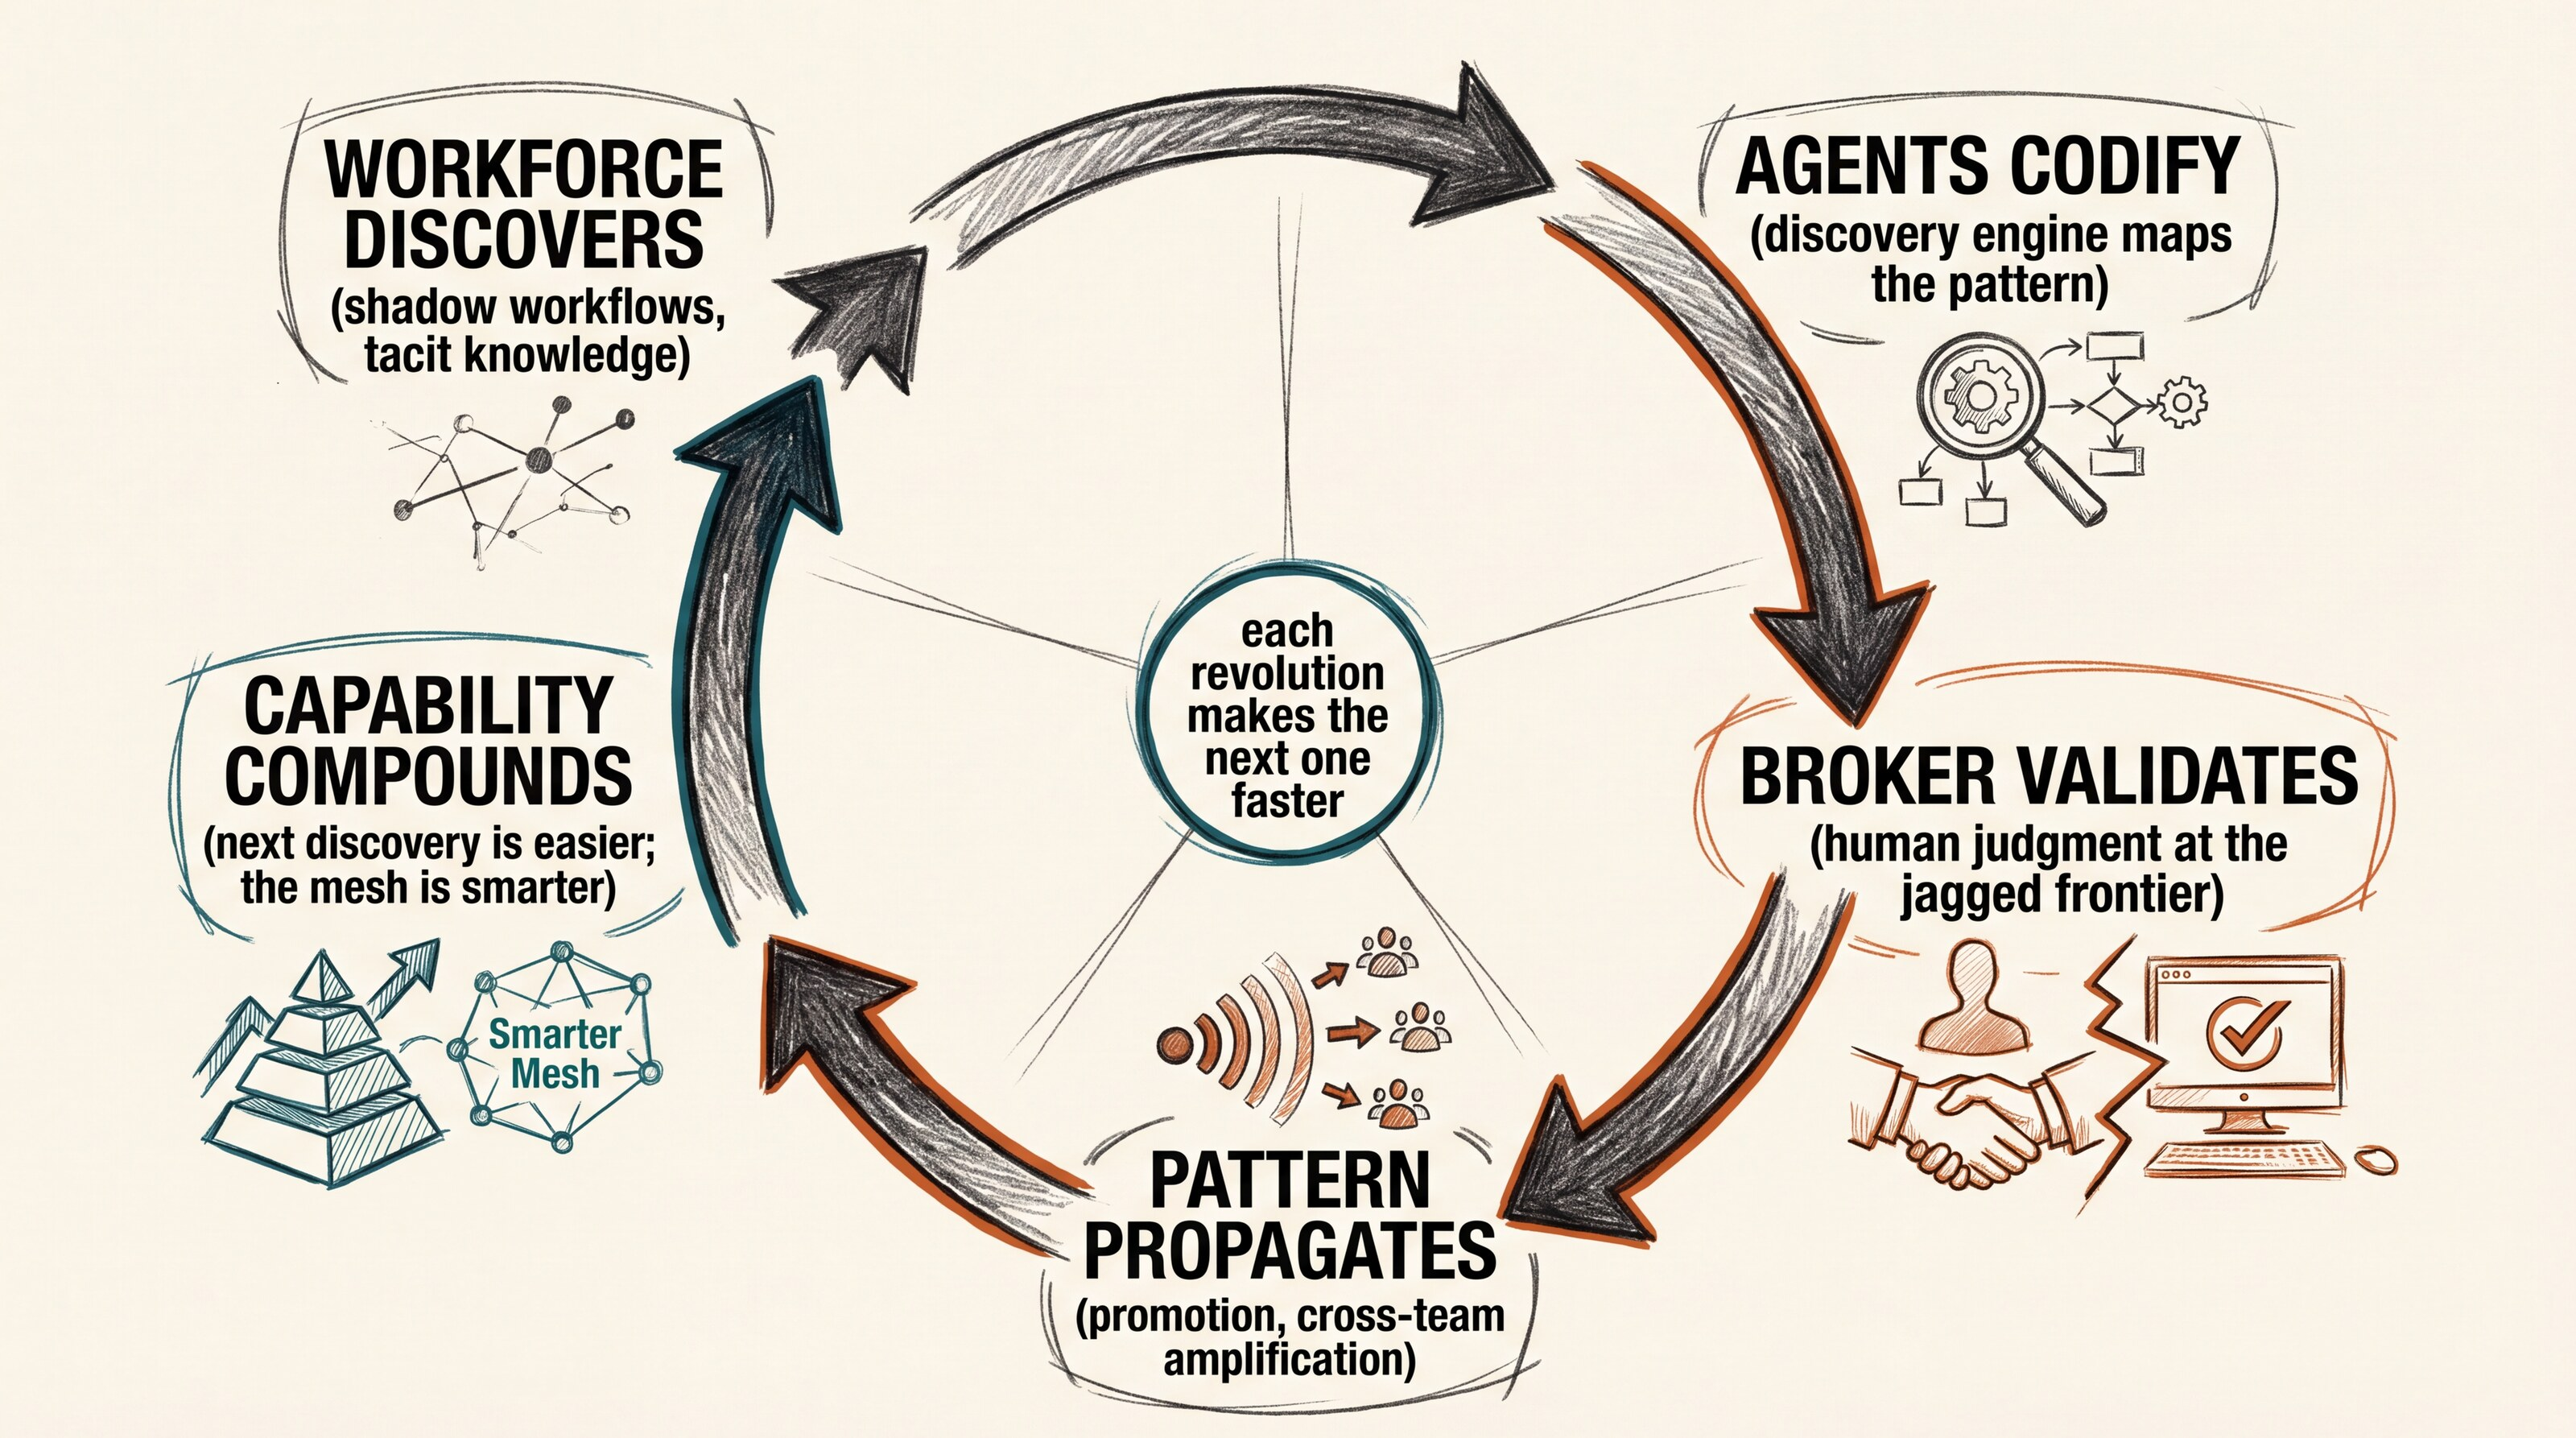
\includegraphics[width=0.9\textwidth]{nb-compound-flywheel.jpg}
\caption{The compound organisational flywheel. Discovery feeds codification; codification feeds validation by the judgment broker; validated workflows propagate through the mesh; propagation increases organisational capability; increased capability accelerates the next cycle of discovery. Each revolution makes the next one faster.}
\label{fig:compound-flywheel-conclusion}
\end{figure}

The flywheel in Figure~\ref{fig:compound-flywheel-conclusion} is the core mechanism of the coordination collapse thesis. It is not a strategy diagram. It is an operational description of how the mesh produces compounding returns. Each shadow workflow surfaced by the Discovery Engine becomes institutional capability through the Insight Ingestion Loop. Each validated DAG makes the mesh smarter. Each cycle of the flywheel reduces the time required for the next cycle --- the metric captured by Mesh Velocity.

The compound flywheel addresses Acemoglu's scepticism about AI productivity gains \parencite{Acemoglu2025}. His 0.66 per cent TFP estimate applies to the economy as a whole. An individual organisation running a compound flywheel captures gains that are disproportionate to the macroeconomic average --- precisely because the gains compound, and because the organisation's competitors have not yet built the flywheel. The strategic advantage is not in using AI. It is in building a system that learns from its own use of AI.

\section{What the Evidence Supports}

The following propositions are supported by the evidence reviewed in this report:

\begin{enumerate}
  \item Hierarchy is an information routing protocol. The coordination tax is real and measurable. AI can perform the information routing function at a fraction of the cost and latency.
  \item The boundary between what AI can and cannot do is jagged, unpredictable, and dynamic \parencite{DellAcqua2026}. Wholesale automation is empirically reckless.
  \item Human oversight degrades as AI quality improves \parencite{DellAcqua2023}. ``Human in the loop'' without architectural support for maintaining vigilance is an unreliable governance mechanism.
  \item Three collaboration modes exist --- Centaur, Cyborg, and Self-Automator. The Self-Automator mode produces the worst outcomes \parencite{Randazzo2024}.
  \item Organisations that revise their KPIs to account for AI are three times more likely to see financial benefit \parencite{BCGAIKPIs2025}.
  \item The 1-9-90 adoption pattern is predictable, and investing in the 9 per cent yields the highest return \parencite{BCGAgenticShift2025}.
  \item Psychological safety is the strongest predictor of successful AI adoption \parencite{EdmondsonLei2025, GoogleAristotle2025}. Protected experimentation time produces 3.1 times higher adoption rates.
  \item Providing sanctioned AI tools reduces unauthorised use dramatically. Ignoring shadow AI is not a neutral choice.
  \item Human-imitation organisational forms underperform agent-native forms in agent collectives; collective efficiency collapses at high contextual transaction cost \parencite{Liu2026}.
  \item Escalation-based oversight outperforms approval-based oversight in production deployments, with 71 versus 30 per cent median productivity gains \parencite{Pereira2026Playbook}.
  \item Multi-agent failure is systematic and taxonomisable, with 41--86.7 per cent failure rates documented in naive frameworks \parencite{Cemri2025}.
  \item Headcount reduction is the most common but not the majority outcome of successful AI deployment: 45 per cent, against 55 per cent for growth, redeployment, and avoided hiring combined \parencite{Pereira2026Playbook, RampRevelio2026}.
\end{enumerate}

\section{What the Evidence Does Not Yet Support}

The following propositions are advanced by this report but not yet validated by independent evidence:

\begin{enumerate}
  \item The full organisational compounding flywheel, where each discovered insight makes the next discovery easier at the systems level, has not been demonstrated at scale.
  \item The proposed KPIs (Mesh Velocity, Augmentation Ratio, Trust Variance, HITL Precision) now have a theoretical anchor in Liu's contextual-transaction-cost and collective-efficiency framework (Chapter~\ref{ch:coordination-economics}), but they remain empirically unvalidated at scale.
  \item The judgment broker role has not been tested with brokers who did not build the underlying system.
  \item The Dynamic Agentic Mesh has not been proven beyond a 15-person team in a favourable context.
  \item The governance architecture (declarative governance, ontological provenance, cascading trust) has not been stress-tested in regulated industries.
  \item The mapping between Liu's simulated organisation forms and production organisational architectures is interpretive, not demonstrated: blackboard memory and adaptive meta-organisation were validated against synthetic tasks and small real-LLM traces, not against functioning enterprise organisations.
  \item The interaction layer is uneven in ways the doctrine does not admit on its own: the gap register (Chapter~\ref{ch:gap-register}) found the governance plane production-real but reserved to administrators, and the embodiment, mixed-reality, and voice surfaces materially behind the canon that describes them.
\end{enumerate}

Acknowledging these gaps is not a weakness. It is a statement of where the research frontier lies and an invitation for others to test the propositions in their own contexts.

\section{Closing Messages}

\subsection{For Middle Managers}

You are not being replaced. You are being promoted, from information router to judgment broker. The promotion is not in title or compensation (those are organisational decisions outside this report's scope). The promotion is in \emph{complexity, scope, and strategic importance}. The skill you need is not technical. It is the willingness to map the jagged frontier in your domain and the judgment to know when to trust the mesh and when to override it.

This is no longer only a projection. Ford rehired approximately 350 veteran ``greybeard'' engineers over three years specifically because AI tooling alone could not sustain quality, and used them to retrain the AI tools themselves, becoming the top mainstream brand in the J.D. Power Initial Quality Study in the process \parencite{Bloomberg2026Ford}. The escalation-model evidence quantifies exactly what the judgment path is worth: production deployments built around human review of exceptions, rather than approval of every output, show 71 per cent median productivity gains against roughly 30 per cent for approval-on-everything models \parencite{Pereira2026Playbook}. The judgment broker is not a hopeful reframing of a shrinking role. It is what the highest-performing deployments already look like.

The organisations that will outcompete are not the ones that eliminate middle management. They are the ones that give their middle managers experimentation time (3.1 times higher adoption), psychological safety (2.6 times more likely to report successful AI integration), and a clear path from coordination to judgment.

Not every current middle manager will make this transition. The 1-9-90 data is honest about that. But the path is real, the evidence supports it, and the role that emerges on the other side is more valuable, more intellectually demanding, and more strategically important than the one it replaces.

\subsection{For Change Managers}

Your playbook is not broken. It is incomplete. AI transformation has no end state. You are not managing a transition; you are building an organisation's capacity for continuous adaptation.

The frameworks exist: Continuous Transformation \parencite{WadeBonnet2025}, Directed Autonomy \parencite{MicrosoftDirectedAutonomy2025}, Dynamic Capabilities \parencite{Teece2025}. The mesh provides the architecture. The 90-day roadmap in Chapter~\ref{ch:implementation} is the bootstrap sequence. Phase 3 never ends. Your job is perpetual, and that is not a burden. It is a description of a role that will be needed for as long as the jagged frontier moves, which is to say permanently.

\subsection{For AI Leaders}

The secret cyborgs are your greatest asset, not your greatest risk. Surface them. Sanction them. Learn from them. The shadow workflows they have already created are the raw material for your compounding loop.

Providing approved tools drops unauthorised use by 89 per cent. The alternative, 1,200 unsanctioned applications per enterprise \parencite{Gartner2025}, \$4.63 million per breach \parencite{IBM2025}, is untenable. The governance paradox has a resolution: embed governance into the architecture, and it becomes an accelerator rather than a brake.

But surfacing shadow workflows requires psychological safety. Workers who have automated 90 per cent of their role will not volunteer that information if they believe it invites headcount reduction. \textcite{Mollick2025Management} is direct on this point: organisations that delegate AI strategy to IT without CEO engagement guarantee failure.

The Stanford Digital Economy Lab's study of 51 successful deployments \parencite{Pereira2026Playbook} converges on the same imperatives from the opposite direction: not theory, but ground truth from organisations that got it right: start with the invisible work, because 77 per cent of the hardest challenges were change management and process redesign, not technology; define your KPIs before deployment, not after; and build multi-model, abstraction-layer architecture from day one, because the durable advantage sits in the orchestration layer, not in any single foundation model. Chapter~\ref{ch:ecosystem-roadmap} turns those same prescriptions on this report's own systems, as a dated schedule of commitments the next edition can mark kept or broken.

\subsection{For All Three}

Block diagnosed the right problem. The question is whether you agree with their prescription. The evidence reviewed in this report suggests you should not. But you should take the diagnosis deadly seriously.

The coordination collapse is real. What you build in its place will determine whether your organisation compounds or collapses.

\vspace{2cm}

\begin{center}
\textcolor{accentgold}{\rule{0.4\textwidth}{1pt}}

\vspace{0.5cm}

{\small\textcolor{navyblue!70!black}{DreamLab AI Consulting Ltd\\
Dr.\ John O'Hare\\
DreamLab, Fairfield, Eskdale\\
July 2026}}
\end{center}


% ─── Back Matter ─────────────────────────────────────────────────────────────
\backmatter

% Bibliography
\printbibliography[heading=bibintoc, title={References}]

% Appendices
\appendix
\chapter{Research Methodology}
\label{ch:methodology}

This appendix documents the research methodology used to produce this report, including the multi-agent research architecture, source selection criteria, codebase audit procedures, and Wardley mapping approach.

\section{Multi-Agent Research Architecture}

The research was conducted using five parallel research agents, each assigned a distinct domain with defined source priorities and quality thresholds. The agents operated concurrently across a shared memory layer (RuVector, 1.17 million vector embeddings with HNSW indexing) that enabled cross-domain pattern detection and prevented duplication of effort.

\begin{table}[H]
\centering
\caption{Research agent assignments and source priorities}
\label{tab:research-agents}
\begin{tabularx}{\textwidth}{l l X}
\toprule
\textbf{Agent} & \textbf{Domain} & \textbf{Primary Sources} \\
\midrule
Agent 1 & Mollick / BCG / Jagged Frontier & \textcite{DellAcqua2026}, \textcite{Randazzo2024}, \textcite{DellAcqua2023}, Mollick's ``One Useful Thing'' corpus, \textcite{BCGAIKPIs2025} \\
\addlinespace
Agent 2 & Block Critique & \textcite{DorseyBotha2026}, \textcite{Zamost2026}, \textcite{Spicer2026}, \textcite{Klarna2025}, \textcite{OrgvueForrester2025} \\
\addlinespace
Agent 3 & Agentic Organisations & \textcite{McKinseyAgenticOrg2026}, \textcite{McKinseySixShifts2026}, \textcite{BCGAgenticShift2025}, \textcite{BCGAgenticEnterprise2025}, \textcite{Deloitte2026} \\
\addlinespace
Agent 4 & Change Management & \textcite{WadeBonnet2025}, \textcite{Teece2025}, \textcite{MicrosoftDirectedAutonomy2025}, \textcite{Prosci2024}, \textcite{Capgemini2025} \\
\addlinespace
Agent 5 & Every / Compound Engineering & \textcite{Shipper2026}, \textcite{Klaassen2025}, \textcite{CyberArk2025}, \textcite{TDS2026} \\
\bottomrule
\end{tabularx}
\end{table}

Each agent maintained a source provenance log in the shared RuVector memory, recording the retrieval date, URL, and a confidence assessment for each source. Cross-referencing between agents was automated through semantic vector search: when Agent 2 (Block Critique) encountered a claim about AI productivity, the memory layer surfaced related findings from Agent 1 (Mollick / BCG) and Agent 5 (Every / Compound) for triangulation.

\section{Source Selection and Quality Assessment}

Sources were categorised into four tiers based on methodological rigour and evidentiary weight.

\subsection{Tier 1: Peer-Reviewed and Pre-Registered Research}

The highest evidentiary weight was assigned to peer-reviewed publications and pre-registered experiments. The primary load-bearing sources in this category are:

\begin{itemize}
  \item \textcite{DellAcqua2026}: pre-registered field experiment with 758 BCG consultants, published in \emph{Organization Science}. This is the evidential foundation for the jagged frontier concept.
  \item \textcite{Randazzo2024}: follow-up study with 244 BCG consultants identifying the Centaur, Cyborg, and Self-Automator collaboration modes.
  \item \textcite{DellAcqua2023}: field experiment with HR recruiters demonstrating the vigilance degradation problem.
  \item \textcite{Acemoglu2019}: the task-based automation framework that grounds the economic analysis of AI and labour.
  \item \textcite{Acemoglu2025}: the sceptical macroeconomic analysis of AI productivity, arguing for at most 0.66 per cent TFP gain over a decade.
\end{itemize}

\subsection{Tier 2: Institutional Research with Disclosed Methodology}

Consultancy reports and institutional research with disclosed sample sizes and methodologies. These carry less evidentiary weight than peer-reviewed work but are treated as credible within stated limitations:

\begin{itemize}
  \item \textcite{BCGAIKPIs2025}: joint research with MIT Sloan, $n = 3{,}000+$ across 25 industries.
  \item \textcite{MicrosoftWorkTrend2024}: large-scale survey with disclosed methodology.
  \item \textcite{WEF2025}: the World Economic Forum's Future of Jobs Report.
  \item \textcite{Capgemini2025}: middle manager resistance patterns with percentage-level findings.
  \item \textcite{EdmondsonLei2025}: psychological safety and AI experimentation, grounded in the established literature on team effectiveness.
\end{itemize}

\textbf{Limitation:} Consultancy reports are produced by organisations with commercial interests in the phenomena they describe. Methodology sections are often absent or sparse. Sample composition and response biases are rarely disclosed. Statistics from these sources are used directionally, to establish trends and orders of magnitude; rather than as precise measurements.

\subsection{Tier 3: Expert Commentary and Primary Accounts}

Expert commentary, practitioner accounts, and journalistic reporting. These provide context and narrative but are not treated as primary evidence:

\begin{itemize}
  \item \textcite{DorseyBotha2026}: primary source for the Block Intelligence Layer model.
  \item \textcite{Shipper2026} and \textcite{Klaassen2025}: primary accounts of the Every agent colony experiment.
  \item \textcite{Mollick2025Management}: expert synthesis from a researcher with deep domain expertise.
  \item \textcite{Spicer2026} and \textcite{Zamost2026}: expert and insider critique of Block.
\end{itemize}

\subsection{Tier 4: Community and Vendor Sources}

Sources with limited editorial oversight or commercial incentives. Used cautiously and flagged where they appear:

\begin{itemize}
  \item \textcite{TDS2026}: the original 17$\times$ error multiplication statistic. Superseded in this edition by \textcite{Cemri2025} (Chapter~\ref{ch:open-questions}); retained here in the bibliography for the correction record, not as an active source.
  \item \textcite{IBM2025} and \textcite{Gartner2025}: vendor-funded research with commercial incentives. Treated as directionally correct, per the methodological note in Chapter~\ref{ch:open-questions}.
\end{itemize}

\section{Web Search and Academic Database Approach}

Research was conducted through a combination of five source channels:

\begin{enumerate}
  \item \textbf{Academic databases}: Google Scholar, SSRN, NBER Working Papers, HBS Working Papers. Search terms included ``agentic organisation,'' ``AI coordination,'' ``human-AI collaboration,'' ``middle management AI,'' ``organisational design automation,'' and ``jagged technological frontier.''
  \item \textbf{Consultancy publication portals}: McKinsey Insights, BCG Publications, Deloitte Insights, Gartner Research. Filtered to 2024--2026 publications on organisational AI.
  \item \textbf{Practitioner platforms}: Substack (particularly Mollick's ``One Useful Thing'' and Every's ``Chain of Thought''), podcasts, and conference proceedings.
  \item \textbf{News and analysis}: Financial Times, New York Times, Fortune, CNBC, VentureBeat. Used for event-driven reporting (Block restructuring, Klarna reversal) with cross-referencing against multiple outlets.
  \item \textbf{Regulatory sources}: EUR-Lex for EU AI Act text, UK Legislation website for the Employment Rights Act, ICO guidance on workplace monitoring.
\end{enumerate}

\section{Codebase Audit Methodology}

The VisionClaw codebase was audited in April 2026 to reconcile claims made in earlier versions of this document against the actual code. The audit procedure:

\begin{enumerate}
  \item \textbf{Claim extraction}: all factual claims about VisionClaw's capabilities were extracted from the document and catalogued.
  \item \textbf{Code search}: each claim was tested against the codebase using structural code analysis (call graphs, dependency trees) and text search. The codebase-memory MCP tool (48,159 nodes, 95,766 edges) was used for structural queries.
  \item \textbf{Verification categories}: each claim was classified as (a) verified and accurate, (b) partially accurate with caveats, or (c) not supported by the code.
  \item \textbf{Correction}: claims in categories (b) and (c) were corrected in Chapter~\ref{ch:technical-substrate}. The corrections are presented transparently, with both the original claim and the corrected version visible.
\end{enumerate}

\begin{cautionbox}[title={Conflict of Interest}]
The codebase audit was conducted by the system architect (Dr.~John O'Hare), who is also the report author and the founder of DreamLab AI Consulting. This introduces a conflict of interest: the auditor has a commercial interest in the system being described favourably. The audit found and corrected seven overclaims (documented in Chapter~\ref{ch:technical-substrate}), which provides some evidence of good faith. Independent code review by a third party would strengthen the credibility of the technical claims but was not available at the time of writing.
\end{cautionbox}

\section{Wardley Mapping Methodology}

Five Wardley maps were produced for this report, each following Simon Wardley's standard mapping methodology:

\begin{enumerate}
  \item \textbf{Value chain identification}: for each map, the user need was identified and the value chain of components required to serve that need was enumerated.
  \item \textbf{Evolution assessment}: each component was placed on the evolution axis (Genesis $\rightarrow$ Custom $\rightarrow$ Product $\rightarrow$ Commodity/Utility) based on its current maturity and market availability.
  \item \textbf{Movement indication}: where components are expected to evolve (e.g., information routing moving from custom toward commodity), movement arrows indicate the direction and anticipated pace.
  \item \textbf{Strategic interpretation}: each map was interpreted for strategic implications relevant to the report's argument.
\end{enumerate}

The maps are interpretive tools, not empirical measurements. The placement of components on the evolution axis reflects the author's assessment informed by the evidence assembled in this report. Different analysts may position components differently, particularly for novel concepts (judgment brokerage, mesh velocity) whose evolutionary stage is inherently uncertain.

\section{The July 2026 Revision}

This edition was produced through a second, distinct research and drafting cycle three months after the first. The process:

\begin{enumerate}
  \item \textbf{Verification.} Four research agents, each with live web search, verified every transcript-derived claim in the April edition against primary sources --- the CAIS blog, arXiv, Bloomberg, the \emph{New York Times}, Ramp's own research publication, and court-reporting coverage of the Hangzhou ruling, correcting names, dates, and figures before any revision text was written. Corrections of substance are flagged explicitly at the point the original claim appears in the main text.
  \item \textbf{Ecosystem exploration.} Three further agents mapped the current state of the VisionClaw, AgentBox, and federation codebases to ground Chapter~\ref{ch:ecosystem-roadmap}, which applies this report's own findings to DreamLab's operational systems.
  \item \textbf{Drafting.} Chapter revisions were produced by section-scoped writing agents working against a single shared evidence brief with fixed citation keys, house style, and verified figures, so that no two chapters could independently introduce inconsistent numbers for the same claim. The drafts were then editorially reviewed for voice, argument continuity, and consistency with chapters outside each agent's assigned scope.
\end{enumerate}

The new sources introduced in this revision were tier-assigned using the same rubric as above:

\begin{itemize}
  \item \textbf{Tier 1}: \parencite{Cemri2025} --- peer-reviewed, NeurIPS 2025, Datasets and Benchmarks Track.
  \item \textbf{Tier 2}: \parencite{Liu2026} (preprint with disclosed methodology, single author); \parencite{Pereira2026Playbook} (disclosed methodology, acknowledged selection bias toward successful deployments); \parencite{RLI2025}, \parencite{CAIS2026RLI}, and \parencite{METR2026} (benchmark reports with disclosed methodology); \parencite{RampRevelio2026} (corporate research, disclosed methodology, correlational with matched controls).
  \item \textbf{Tier 3}: news reporting --- \parencite{Challenger2026}, \parencite{NYTChina2026}, \parencite{Bloomberg2026Ford}, \parencite{Chatterji2026}.
  \item \textbf{Tier 4}: \parencite{Levie2026}, a single social-media source with no published methodology, flagged wherever it is used.
\end{itemize}

\section{The Third Edition: the Gap-Analysis Mesh}

The third edition's principal new evidence artefact is the four-surface gap register (Chapter~\ref{ch:gap-register}). It was produced by a twelve-agent analysis mesh arranged in two layers, run on 8 July 2026, followed by a separate ten-agent drafting pass.

\textbf{Evidence layer (eight agents).} One agent extracted the ecosystem's espoused doctrine from the VisionFlow canon --- the claims the documentation actually commits to, with file-level citations. Four agents surveyed practice, one per interaction surface (forum, desktop, mixed reality, voice), verifying every capability claim against the running codebases and classifying each as working, partial, scaffolded, docs-only, or absent. Three agents researched external theory and the 2025--26 practice landscape through deliberately independent search channels: a closed synthesis engine, an open multi-source engine with citation verification against academic databases, and a high-recall keyword engine. The three theory agents did not coordinate and their briefs were identical; convergence across them was treated as a signal of consensus in the literature, divergence as a flag for editorial caution.

\textbf{Judgment layer (four agents).} One judge per surface crossed the three inputs --- external theory, espoused canon, verified practice, and recorded gaps typed by which pair diverged: theory-to-canon (published knowledge the doctrine never adopted), canon-to-practice (doctrine promises the code does not deliver), and theory-to-practice (absent from both). Judges were required to re-verify, by reading code, the claims their highest-severity findings depended on, and to check each candidate finding against the prior May 2026 audit so that already-known gaps were marked as still open rather than presented as new.

\textbf{Drafting.} The new chapters of Parts~\ref{part:solution-space}--\ref{part:next-steps} were then written by ten section-scoped writing agents working against a single binding style brief --- house voice, a prose-quality rule set, fixed citation keys, and an instruction hierarchy that ranks the code-verified surveys above aspirational documentation wherever they conflict. New bibliography entries were restricted to sources surfaced with checkable URLs during the theory research; a writer finding no source for a claim was instructed to state it as this report's own analysis or cut it. The drafts received a single-editor review for argument continuity and cross-chapter consistency.

\textbf{Ontology grounding.} The pervasive ontology binding described in Chapter~\ref{ch:ontology-binding} was active throughout production. Its fail-open contract was exercised in the field during this edition's production: the knowledge-graph backend was unreachable during one working session, every retrieval degraded to empty, and the work continued from documentation --- an observed instance of the design behaving as specified, recorded in that chapter.

\begin{cautionbox}[title={Limits of the Mesh Method}]
The analysis mesh shares a single foundation-model family. \textcite{Liu2026}'s pseudo-diversity result --- that same-model, same-tooling reviewers approximate one judge asked several times. This applies to this analysis as much as to any system it audits. The three search channels diversify retrieval, and the code-verification requirement anchors findings to artefacts rather than opinion, but the judgment layer is not model-diverse, and the auditor remains the audited organisation. The register's severity ratings should be read with both caveats attached.
\end{cautionbox}

\subsection{Weaving in the 2022 Baseline}

A separate tiered swarm produced the material that connects this report to the author's 2022 monograph \parencite{OHare2022Convergence}, disclosed in the introduction (Chapter~\ref{ch:introduction}) and audited in Chapter~\ref{ch:2022-wager}. It ran in four ranked stages, each narrower and more senior than the one before.

\textbf{Scouts (sixteen agents).} Sixteen Haiku agents read the 42 LaTeX source files of the 2022 book, a handful each, and extracted candidate continuity threads (passages on identity, Bitcoin, Lightning, decentralised organisations, mixed reality and language models that prefigured a 2026 component) with file-level citations and no ruling on strength.

\textbf{Synthesists (four agents).} Four Sonnet agents consolidated the scout output into a single lineage map, typing each thread by evidential strength: verbatim-level continuity, strong on mechanism but loose on narrative, and thematic only. Threads that could not be tied to a specific 2022 passage were dropped.

\textbf{Integrators (five agents).} Five Opus agents wove the surviving threads into the existing chapters as additive sentences, under the report's disclosure discipline: state the code-verified 2026 fact first, then name its 2022 ancestry, and retrofit no continuity that reads as marketing. Each integrator was scoped to a fixed set of files so that no two edited the same passage in parallel.

\textbf{Editor (single pass).} One editor reconciled voice across the insertions, cut overclaims, and required every continuity sentence to point forward to the chapter carrying the code-verified detail rather than restating it.

Two standing resources grounded the pass beyond the 2022 text. The operator's RuVector memory, through its \texttt{personal-context} and \texttt{project-state} namespaces, supplied the verified authorial history (the telepresence doctorate and the Octave mixed-reality laboratory tenure) that keeps the continuity claims accurate without inflating them. The pervasive ontology binding of Chapter~\ref{ch:ontology-binding}, active here as it was for the gap-analysis mesh, bound recurring terms such as the identity keypair, the block-trail and the judgment broker to their governed definitions, so the 2022-to-2026 mapping ran on one vocabulary at both ends.

\section{Limitations of the Research Process}

\begin{enumerate}
  \item \textbf{Single-author synthesis}: while the research was conducted using multiple agents, the synthesis and editorial judgment are those of a single author. The report reflects one analytical perspective on a multi-faceted phenomenon.
  \item \textbf{Temporal constraints}: this edition incorporates sources through early July 2026; sources published after that point are not included. The jagged frontier, in particular, continues to shift --- the Remote Labor Index update alone recorded a 6.4-fold increase in client-quality automation in the eight months preceding this revision \parencite{CAIS2026RLI}, and there is no reason to expect the pace to slow before the next edition.
  \item \textbf{English-language bias}: the research draws almost exclusively on English-language sources. Organisational innovations in non-Anglophone contexts, particularly Haier's micro-enterprise model in China, are discussed secondhand rather than from primary sources.
  \item \textbf{Analyst-vendor conflict}: the author is the founder of DreamLab AI Consulting and the architect of VisionClaw. This conflict is acknowledged throughout the report and addressed directly in Chapter~\ref{ch:open-questions}.
  \item \textbf{Sample bias in practitioner evidence}: the Every experiment ($\sim$20 people) and VisionClaw deployment ($\sim$15--50 people) are both small-scale, technically sophisticated organisations. The generalisability of findings from these contexts to larger, less technical organisations is an open question.
\end{enumerate}

\section{Disclosure}

The author of this report, Dr.\ John O'Hare, is the founder and principal of DreamLab AI Consulting Ltd and the architect of the VisionClaw system described in Chapter~\ref{ch:technical-substrate}. The report simultaneously analyses the problem space, proposes a solution framework, and describes a commercial offering from the author's firm. This positioning conflict is acknowledged in Chapter~\ref{ch:open-questions} and is offered as context for the reader's own evaluation of the argument.

\input{appendices/appendix-b-competitor-matrix}
\input{appendices/appendix-c-glossary}

\end{document}
